\documentclass[11pt,spanish,a4paper,twoside,openany]{book}
\raggedbottom
% descomentar para debuggear overfull warnings:
% \overfullrule=1mm

\usepackage[
  active=true,
  header=true,
  generate=ejercicios.tex,
  copydocumentclass=false,
  extract-env=ejercicio,
  ejercicio-labels={guia},
  extract-cmd=chapter,
  chapter-nrs={1-9,11,14,16-20},
]{extract}

% Document class para ejercicios.tex.
\begin{extract}
\documentclass[11pt,a4paper]{article}
\end{extract}

% Preámbulo compartido entre apunte y ejercicios.
\begin{extract*}
\tolerance=5000

% Entrada de texto
\usepackage{polyglossia}
\setmainlanguage{spanish}

% Cuestiones de estilo
\usepackage{listings}         % Permite mostrar codigo de forma mas linda
\usepackage{verbatim}         % Permite incluir archivos de texto verbatim

\usepackage{amsmath, amsthm, amssymb} % Se usan para theoremstyle

\usepackage{relsize}
\newcommand{\dificil}{\mathlarger{\mathlarger{\star}}}

\usepackage[table]{xcolor}
\definecolor{light-gray}{gray}{0.96}
\definecolor{med-gray}{gray}{0.8}

\definecolor{keyword}{rgb}{0,0,0.5}
\definecolor{string}{rgb}{0.5,0,0.5}
\definecolor{error}{rgb}{0.5,0,0}

% para poder usar upquote=true (mostrar bien las comillas simples)
\usepackage{textcomp}

\usepackage[labelfont=bf]{caption}

% Parámetros para los listings de python
\lstset{
    language=Python,
    columns=fixed,
    keepspaces=true,
    numbers=left,
    tabsize=4,
    numberstyle=\color{gray}\tiny\ttfamily,
    numbersep=5pt,
    showstringspaces=false,
    basicstyle=\small\ttfamily,
    keywordstyle=\color{keyword},
    backgroundcolor=\color{light-gray},
    commentstyle=\color{gray},
    stringstyle=\color{string},
    morecomment=[s]{>>}{>}, % hack para pintar los prompts >>>
    morecomment=[s]{..}{.}, % y ...
    xleftmargin=\dimexpr\parindent+10pt,
    breaklines=true,
    postbreak=\lst@ifdisplaystyle{\raisebox{0ex}[0ex][0ex]{\ensuremath{\hookrightarrow\space}}}\fi,
}

\lstdefinestyle{inlinecode}{
    backgroundcolor=\color{light-gray}
}

% Para poner partes dentro de los ejercicios
\newcounter{partesi}
\newenvironment{partes}
{   \begin{list}{\alph{partesi})}{
        \usecounter{partesi}
        \setlength{\topsep}{0pt}
        \setlength{\itemsep}{0pt}}}
{   \end{list} }

\usepackage{unicode-math}

\setmainfont
     [ BoldFont       = texgyrepagella-bold.otf ,
       ItalicFont     = texgyrepagella-italic.otf ,
       BoldItalicFont = texgyrepagella-bolditalic.otf ]
     {texgyrepagella-regular.otf}
\setmathfont[Scale=MatchLowercase]{texgyrepagella-math.otf}
\usepackage{DejaVuSansMono}
\setmonofont[Scale=0.9]{DejaVuSansMono}

\usepackage{array}            % Permite alinear los párrafos en las celdas verticalmente
\usepackage{enumitem}
\setlist{labelindent=\parindent, leftmargin=*, align=left, topsep=1.25\parsep,
itemsep=0.5\parsep}

\end{extract*}

% Resto del preámbulo de ejercicios.tex
\begin{extract}

\renewcommand{\baselinestretch}{1.3}

\oddsidemargin 0.0cm \evensidemargin 0.0cm \topmargin 0in
\headheight .3in \headsep .2in \footskip .2in
\setlength{\textwidth}{16cm}
\setlength{\textheight}{22cm}
\topmargin 0.5 cm

\theoremstyle{definition}
\newtheorem{ejercicio}{Ejercicio}[section]

% Para poder usar los nombres de capítulos como secciones.
% TODO: al omitir capítuos en los ejercicios, las secciones en los ejercicios
% se siguen numerando consecutivamente, y se desacoplan del número de capítulo.
\newcommand{\chapter[2]}{\section{#2}}

\title{75.40 Algoritmos y Programación I \\
    \textbf{Guía de Ejercicios}}
\date{2.\textsuperscript{do} cuatrimestre 2019}

\usepackage{url}              % Para incluir URLs
\end{extract}

%% Resto del preámbulo solo definido para el apunte. %%

\usepackage[title,titletoc]{appendix}

\usepackage{graphicx}         % Permite insertar imagenes.

\usepackage{longtable}        % tablas largas y flexibles
\usepackage{nonfloat}         % Hace que las figuras no floten
\usepackage{eso-pic}

% Margenes y largo del texto
%
% medidas horizontales
% 1in(fijo) + \hoffset + \(odd|even)sidemargin + \textwidth + \marginparsep +
% \marginparwidth + \marginparpush
%
% medidas verticales
% 1in(fijo) + \voffset + \topmargin + \headheight + \headsep + \textheight +
% \footskip

\setlength\oddsidemargin{-0.04cm}
\setlength\evensidemargin{-0.04cm}
\setlength\topmargin{0cm}
\setlength\headheight{0.5cm}
\setlength\headsep{0.3cm}
\setlength\footskip{0.8cm}
\setlength\textwidth{16cm}  % ancho para apunte
\setlength\textheight{23cm} % largo para apunte

\usepackage{fancyhdr}         %
\pagestyle{fancy}
\fancyhf{} % clear all header and footer fields
\fancyhead[RO]{\slshape \rightmark \hspace{1cm} \normalfont \bfseries \thepage}
\fancyhead[LE]{\bfseries \thepage \hspace{1cm} \normalfont \leftmark}
\renewcommand{\headrulewidth}{0.3pt}
\renewcommand{\footrulewidth}{0pt}

\fancypagestyle{plain}{%
\fancyhf{} % clear all header and footer fields
\renewcommand{\headrulewidth}{0pt}
\renewcommand{\footrulewidth}{0pt}}

\renewcommand{\sectionmark}[1]{\markright{\thesection.\ #1}}
\renewcommand{\chaptermark}[1]{\markboth{\chaptername\ \thechapter.\ #1}{}}

\usepackage{color}            % Permite definir colores
\definecolor{rosa}{rgb}{1,0.90,0.90}
\definecolor{celeste}{rgb}{0.90,0.90,0.95}
\definecolor{verde}{rgb}{0.85,1.00,0.85}
\definecolor{amarillo}{rgb}{1.00,1.00,0.75}

\usepackage[framemethod=tikz]{mdframed}
\usepackage{pgfplots}

\newmdenv[
    font=\small,
    linewidth=0,
    backgroundcolor=celeste,
    nobreak=true
]{observacion}

\newlength{\currentparskip}
\newlength{\currentparindent}

\newenvironment{sabias_que}
{\setlength{\currentparskip}{\parskip}%
\setlength{\currentparindent}{\parindent}%
\begin{figure*}[h!t]\begin{mdframed}[
    font=\small,
    linecolor=black,
    backgroundcolor=verde,
    frametitlefont=\normalsize\bfseries,
    frametitle={$\vcenter{\hbox{
\includegraphics[height=4ex]{graficos/lamparita}}}$ Sabías que\ldots},
    frametitlealignment={\hspace*{-\parindent}},
    startinnercode={\setlength{\parskip}{\currentparskip}\setlength{\parindent}{\currentparindent}}
]}{\end{mdframed}\end{figure*}}

\newmdenv[
    font=\small,
    linecolor=black,
    backgroundcolor=amarillo,
    frametitlefont=\normalsize\bfseries,
    frametitle={$\vcenter{\hbox{
\includegraphics[height=3ex]{graficos/atencion}}}$ Atención},
    frametitlealignment={\hspace*{-\parindent}},
    nobreak=true
]{atencion}

\newmdenv[
    font=\small,
    backgroundcolor=verde,
    hidealllines=true,
    frametitlerule=true,
    frametitlefont=\normalsize\bfseries,
    frametitle={Referencia Python\hfill$\vcenter{\hbox{
\includegraphics[height=4ex]{graficos/logo-python}}}$},
    frametitlealignment={\hspace*{-\parindent}},
	needspace=10\baselineskip
]{referencia_python}

\newenvironment{sintaxis}[1]
  {\needspace{2\baselineskip}\mdfsubtitle[
    subtitlebackgroundcolor=verde,
    subtitleaboveskip=4pt,
    subtitlebelowskip=8pt,
    subtitleinneraboveskip=8pt,
    subtitleinnerbelowskip=0pt
  ]{#1}\parskip=0pt}
  {}

\usepackage{float}            % Agrega estilos a los floats

\floatstyle{ruled}
\newfloat{codigo-float}{htbp}{lop}[chapter]
\floatname{codigo-float}{Código}

\newcommand{\lsthighlight}{\lstset{
    moredelim=**[is][\bfseries]{(@}{@)},
    moredelim=[is][\color{error}]{(^}{^)},
    escapeinside={(~}{~)}
}}
\newcommand{\lstnonumbers}{\lstset{
    numbers=none,
    xleftmargin=\parindent
}}

\newenvironment{codigo}[2]{\begin{codigo-float}
    \caption{{\small\texttt{#1}}\textbf{:}\ \small #2}
    }{\end{codigo-float}}

\lstnewenvironment{codigo-python}{\lsthighlight}{}
\lstnewenvironment{codigo-python-sn}{\lsthighlight\lstnonumbers}{}
\lstnewenvironment{codigo-python-sn-small}{\lsthighlight\lstnonumbers\lstset{basicstyle=\footnotesize\ttfamily}}{}
\lstnewenvironment{codigo-nohl}{\lstset{language={}}\lsthighlight}{}
\lstnewenvironment{codigo-nohl-sn}{\lstset{language={}}\lsthighlight\lstnonumbers}{}

\newcommand{\tituloCodigo}[1]{
\bigskip
\needspace{4cm}
\hrule
\smallskip
{\noindent #1}
\smallskip
\hrule
}

% Numeracion para secciones y subsecciones - Hace falta?
\renewcommand{\thesection}{\thechapter.\arabic{section}}
\renewcommand{\thesubsection}{\thesection.\arabic{subsection}}

% Estilos usados en el texto
\theoremstyle{definition}
\newtheorem{definicion}{Definici\'on}[section]
\newtheorem{ejemplo}{Ejemplo}[section]
\newtheorem{problema}{Problema}[section]
\newtheorem{ejercicio}{Ejercicio}[section]
\newtheorem{ejerciciof}{}[section]
\newtheorem{problemac}{Problema}[chapter]
\newtheorem{ejercicioc}{Ejercicio}[chapter]
\renewcommand{\qedsymbol}{} % El proof inserta dos qed al final
\newenvironment{solucion}[1][Solución]{\begin{proof}[#1]}{\end{proof}}

\theoremstyle{remark}
\newtheorem*{nota}{Nota}

% Traducciones propias
\addto\captionsspanish{
\renewcommand{\chaptername}{Unidad}
\renewcommand{\contentsname}{Contenidos}
}

\def\ra{\rightarrow}

% Para tener hiperlinks, en el panel lateral y en la toc.
\usepackage[xetex,unicode=false,setpagesize=false,colorlinks]{hyperref}
\hypersetup{%
	linkcolor=black,
	urlcolor=blue,
	pdftitle={Algoritmos y Programación I - Aprendiendo a programar usando Python como herramienta},
	bookmarksnumbered,
}%
\usepackage{hypcap}

\usepackage{menukeys}

\usepackage{tikz}
\usetikzlibrary{calc,shapes,arrows,babel,trees,fit,positioning}
\newcommand{\tikzmark}[1]{\tikz[overlay,remember picture] \node (#1) {};}

\tikzset{
    umlattr/.style={right,node font=\ttfamily,draw=none,fill=none,node distance=0pt},
    umltitle/.style={node font=\ttfamily,draw=none,fill=none,node distance=0pt},
    umlattrs/.style={draw=none,fill=none,inner sep=0pt},
    umlclass/.style={draw,fill=none,inner sep=0pt},
    flecha/.style={draw,->,>=latex},
    decision/.style={diamond,draw,aspect=2},
    bloque/.style={rectangle,draw},
    start/.style={circle,draw},
    end/.style={circle,draw,fill},
}

\newcommand*\circled[1]{\tikz[]{
  \node[shape=circle,font=\ttfamily,draw,fill=black,text=white,inner sep=0.5pt] (char) {\tiny{#1}};}}

\usepackage{multirow}

\begin{document}

%\AddToShipoutPictureBG*{%
%  \AtPageLowerLeft{%
%    \hspace{\baselineskip}%
%    \raisebox{\baselineskip}{%
%      \makebox[0pt][l]{Última revisión: \today}}}}

\begin{extract*}
\lstMakeShortInline[style=inlinecode]|
\end{extract*}

\begin{extract} % La guía de estilo para los ejercicios
\maketitle
\thispagestyle{empty}

\newpage

\section*{Recomendaciones al realizar las guías.}

\textbf{Generales:}
\begin{itemize}
	\item Sea claro y prolijo. Es muy importante que el código sea lo más claro y legible posible.
	\item Es muy importante que los identificadores de funciones y variables sean coherentes. El identificador debe ser suficientemente descriptivo.
	\item Ponga una línea en blanco entre las definiciones de función para simplificar la lectura del programa.
	\item Las expresiones matemáticas complejas pueden representarse en varios pasos.
	\item Los ejercicios marcados con el símbolo $\dificil$ son más difíciles y no son de resolución obligatoria.
\end{itemize}

\textbf{Documentación:}
\begin{itemize}
	\item Documente correctamente las funciones y módulos que desarrolle.
	\item Documente partes del código cuyo significado pudiera no quedar del todo claro.
	\item No documente en exceso, pero tampoco ahorre documentación necesaria. La documentación debe ser breve y concisa.
\end{itemize}
\end{extract}

\title{{\bf Algoritmos y Programación I} \\ Aprendiendo a programar usando Python como herramienta}
\date{2\textsuperscript{da} edición}
\maketitle

\chapter*{Prólogo}
\addcontentsline{toc}{chapter}{Prólogo}

Durante mucho tiempo nos preguntamos cómo diseñar un curso de Algoritmos y Programación I
(primera materia de programación de las carreras de Ingeniería en Informática y Licenciatura
en Análisis de Sistemas de la Facultad de Ingeniería de la UBA) que al mismo tiempo fuera
atractivo para los futuros profesionales de la informática, les permitiera aprender a resolver
problemas, y atacara muy directamente el problema de la deserción temprana de estudiantes.


Muchos de los estudiantes que ingresan a primer año de las carreras de informática en nuestro
país lo hacen sin saber programar pese a ser nativos digitales, para los cuales las computadoras
y muchos programas forman parte de su vida cotidiana. El primer curso de programación plantea
entonces varios desafíos: enseñar una metodología para la resolución de problemas, un lenguaje
formal para escribir los programas, y al mismo tiempo hacer que los estudiantes no se sientan
abrumados, tengan éxito en este primer esfuerzo y se sientan atraídos por la posibilidad de
escribir sus propios programas.


En este sentido, la elección del lenguaje de programación para dicho curso no es un tema menor:
el problema radica en elegir un lenguaje que al mismo tiempo sea suficientemente expresivo, tenga
una semántica clara y cuyas complicaciones sintácticas sean mínimas.


Hacía tiempo que buscábamos un lenguaje con todas estas características cuando, durante el debate
posterior a un panel sobre programación en el nivel que tuvo lugar en la conferencia Frontiers in
Engineering Education 2007 organizada por la IEEE, el Dr. John Impagliazzo, de Hofstra University,
relató cómo sus cursos habían pasado de duras experiencias, con altas tasas de deserción, a una
situación muy exitosa, por el solo hecho de haber cambiado el lenguaje de programación de ese curso
de Java a Python. Después de ese estimulante encuentro con Impagliazzo nos pusimos manos a la obra
para diseñar este curso. Fue una grata sorpresa enterarnos también de que el venerable curso de
programación de MIT también había migrado a Python: todo hacía pensar que nuestra elección de lenguaje
no era tan descabellada como se podía pensar.


Este libro pretende entonces ser una muy modesta contribución a la discusión sobre cómo enseñar a
programar en primer año de una carrera de Informática a través de un lenguaje que tenga una suave
curva de aprendizaje, de modo tal que este primer encuentro le resulte a los estudiantes placentero
y exitoso, sin que los detalles del lenguaje los distraiga del verdadero objetivo del curso: la resolución
de problemas mediante computadoras.

\section*{Agradecimientos}

Queremos agradecer a la Facultad de Ingeniería (en particular a su Comisión de Publicaciones) y a
Eudeba por la publicación de este libro. Pero también a todos los que apoyaron desde un primer momento
la escritura y mejora continua de lo que fueron durante varios años las notas de nuestro curso de
Algoritmos y Programación I: a la Comisión Curricular de la Licenciatura en Análisis de Sistemas y al
Departamento de Computación (y a su director, Gustavo López) por apoyar la iniciativa de dar este curso
como piloto, a quienes leyeron y discutieron los manuscritos desde sus primeras versiones y colaboraron
con el curso (Melisa Halsband, Alberto Bertogli, Sebastián Santisi, Pablo Antonio, Pablo Najt,
Leandro Ferrigno, Martín Albarracín, Gastón Kleiman, Matías Gavinowich), a quienes fueron primero alumnos y
luego colaboradores de esta experiencia educativa
(Agustín Santiago,
Alejandro Levinas,
Ana Czarnitzki,
Ariel Vergara,
Bruno Merlo Schurmann,
Damián Schenkelman,
Daniela Riesgo,
Daniela Soto,
Débora Martín,
Diego Alfonso,
Emiliano Sorbello,
Ezequiel Genender,
Fabricio Pontes Harsich,
Fabrizio Graffe,
Federico Barrios,
Federico Esteban,
Federico López,
Florencia Álvarez Etcheverry,
Gastón Goncalves,
Gastón Martínez,
Ignacio Garay,
Ignacio Sueiro,
Javier Choque,
Jennifer Woites,
Juan Costamagna,
Lucas Perea,
Manuel Battan,
Manuel Soldini,
Manuel Porto,
Martín Buchwald,
Martín Coll,
Milena Farotto,
Nicolás Poncet,
Pablo Musumeci,
Robinson Fang),
a los amigos que, como Pablo Jacovkis, Elena García y Alejandro Tiraboschi se ofrecieron a
revisar manuscritos y a hacer sugerencias, y a todos los alumnos de nuestro curso de Algoritmos y
Programación I de la FIUBA que, desde 2009, han usado este texto y nos han ayudado a mejorarlo permanentemente.
De todos modos, por supuesto, los errores son nuestra responsabilidad.


\hfill Buenos Aires, diciembre de 2012.


\tableofcontents
\chapter[Conceptos básicos]{Algunos conceptos básicos}
\label{chapter:conceptos}

En esta unidad hablaremos de lo que es un programa de
computadora e introduciremos unos cuantos conceptos referidos a la
programación y a la ejecución de programas. Utilizaremos en todo
momento el lenguaje de programación Python para ilustrar esos
conceptos.

\section{Computadoras y programas}

En la actualidad, la mayoría de nosotros utilizamos computadoras
permanentemente: para mandar correos electrónicos, navegar por Internet,
chatear, jugar, escribir textos.

Las computadoras se usan para actividades tan disímiles como predecir las
condiciones meteorológicas de la próxima semana, guardar historias clínicas,
diseñar aviones, llevar la contabilidad de las empresas o controlar una
fábrica. Y lo interesante aquí (y lo que hace apasionante a esta carrera) es
que el mismo aparato sirve para realizar todas estas actividades: uno no
cambia de computadora cuando se cansa de chatear y quiere jugar al solitario.

Muchos definen una computadora moderna como ``una máquina que
almacena y manipula información bajo el control de un programa que
puede cambiar''. Aparecen acá dos conceptos que son claves: por un
lado se habla de una {\it máquina} que almacena información, y por
el otro lado, esta máquina está controlada por {\it un programa
que puede cambiar}.

Una calculadora sencilla, de esas que sólo tienen 10 teclas para
los dígitos, una tecla para cada una de las 4 operaciones, un
signo igual, encendido y CLEAR, también es una máquina que
almacena información y que está controlada por un programa. Pero
lo que diferencia a esta calculadora de una computadora es que en
la calculadora el programa no puede cambiar.

Un {\it programa de computadora} es un conjunto de {\it
instrucciones} paso a paso que le indican a una computadora cómo
realizar una tarea dada, y en cada momento uno puede elegir
ejecutar un programa de acuerdo a la tarea que quiere realizar.

Las instrucciones se deben escribir en un lenguaje que nuestra
computadora entienda. Los lenguajes de programación son
lenguajes diseñados especialmente para dar
órdenes a una computadora, de manera exacta y no ambigua. Sería
muy agradable poder darle las órdenes a la computadora en
castellano, pero el problema del castellano, y de las lenguas
habladas en general, es su ambigüedad:

Si alguien nos dice {\it ``Comprá el collar sin monedas''}, no sabremos
si nos pide que compremos el collar que no tiene monedas, o que compremos
un collar y que no usemos monedas para la compra. Habrá que preguntarle
a quien nos da la orden cuál es la interpretación correcta. Pero tales
dudas no pueden aparecer cuando se le dan órdenes a una computadora.

Este curso va a tratar precisamente de cómo se escriben programas
para hacer que una computadora realice una determinada tarea.
Vamos a usar un lenguaje específico (Python) porque es sencillo y
elegante, pero éste no será un curso de Python sino un curso de
programación.

\begin{sabias_que}
Existe una gran cantidad de programas desarrollados en Python, desde
herramientas para servidores, como {\bf mailman}, hasta programas amigables
para usuarios finales, como {\bf emesene}, pasando por aplicaciones
empresariales, {\bf openerp}, {\bf tryton}; herramientas de desarrollo,
{\bf meld}, {\bf mercurial}, {\bf bazaar}, {\bf trac}; plataformas web,
{\bf django}, {\bf turbogears}, {\bf zope}; clientes de bittorrent, {\bf
bittorrent}, {\bf bittornado}, {\bf deluge}; montones de juegos de todo
tipo, y muchísimas aplicaciones más.

Estos programas mencionados son software libre, por lo que se puede obtener y
estudiar el código con el que están hechos.
\end{sabias_que}

\section{El mito de la máquina todopoderosa}

Muchas veces la gente se imagina que con la computadora se puede
hacer cualquier cosa; o que si bien hubo tareas que no eran posibles de
realizar hace 50 años, sí lo serán cuando las computadoras crezcan en poder 
(memoria, velocidad), y se vuelvan máquinas todopoderosas.

Sin embargo eso no es así: existen algunos problemas, llamados
{\it no computables} que nunca podrán ser resueltos por una
computadora digital, por más poderosa que ésta sea. La
computabilidad es la rama de la computación que se ocupa de
estudiar qué tareas son computables y qué tareas no lo son.

De la mano del mito anterior, viene el mito del lenguaje
todopoderoso: hay problemas que son no computables porque en
realidad se utiliza algún lenguaje que no es el apropiado.

En realidad todas las computadoras pueden resolver los mismos
problemas, y eso es independiente del lenguaje de programación que
se use. Las soluciones a los problemas computables se pueden
escribir en cualquier lenguaje de programación. Eso no significa
que no haya lenguajes más adecuados que otros para la resolución
de determinados problemas, pero la adecuación está relacionada con
temas tales como la elegancia, la velocidad, la facilidad para
describir un problema de manera simple, etc., nunca con la
capacidad de resolución.

Los problemas no computables no son los únicos escollos que se le
presentan a la computación. Hay otros problemas que si bien son
computables demandan para su resolución un esfuerzo enorme en
tiempo y en memoria. Estos problemas se llaman {\it intratables}.
El análisis de algoritmos se ocupa de separar los problemas
tratables de los intratables, encontrar la solución más barata
para resolver un problema dado, y en el caso de los intratables,
resolverlos de manera aproximada: no encontramos la verdadera
solución porque no nos alcanzan los recursos para eso, pero
encontramos una solución bastante buena y que nos insume muchos
menos recursos (el orden de las respuestas de Google a una
búsqueda es un buen ejemplo de una solución aproximada pero no
necesariamente óptima).

En este curso trabajaremos con problemas no sólo computables sino
también tratables. Y aprenderemos a medir los recursos que nos
demanda una solución, y empezaremos a buscar la solución menos
demandante en cada caso particular. \\

Algunos ejemplos de los problemas que encararemos y de sus
soluciones:

\begin{problemac}
Dado un número $N$ se quiere calcular $N^{33}$.
\end{problemac}

Una solución posible, por supuesto, es hacer el producto $N \times
N \times \ldots \times N$, que involucra 32 multiplicaciones.

Otra solución, mucho más eficiente es:
\begin{itemize}
\item Calcular $N \times N$.

\item Al resultado anterior mutiplicarlo por sí mismo con lo cual
ya disponemos de $N^{4}$.

\item Al resultado anterior mutiplicarlo por sí mismo con lo cual
ya disponemos de $N^{8}$.

\item Al resultado anterior mutiplicarlo por sí mismo con lo cual
ya disponemos de $N^{16}$.

\item Al resultado anterior mutiplicarlo por sí mismo con lo cual
ya disponemos de $N^{32}$.

\item Al resultado anterior mutiplicarlo por $N$ con lo cual
conseguimos el resultado deseado con sólo 6 multiplicaciones.

\end{itemize}

Cada una de estas dos soluciones representa un {\it algoritmo}, es
decir un método de cálculo, diferente. Para un mismo problema
puede haber algoritmos diferentes que lo resuelven, cada uno con
un costo distinto en términos de recursos computacionales
involucrados.

\begin{sabias_que}
La palabra \textit{algoritmo} no es una variación de \textit{logaritmo},
sino que proviene de \textit{algorismo}. En la antigüedad, los
\textit{algoristas} eran los que calculaban usando la numeración arábiga y
mientras que los \textit{abacistas} eran los que calculaban usando ábacos.
Con el tiempo el \textit{algorismo} se deformó en \textit{algoritmo},
influenciado por el término \textit{aritmética}.

A su vez, el uso de la palabra \textit{algorismo} proviene del nombre de un
matemático persa famoso, en su época y para los estudiosos de esa época,
Abu Abdallah Muhammad ibn Mûsâ al-Jwârizmî, que literalmente significa:
``Padre de Ja'far Mohammed, hijo de Moises, nativo de Jiva''. Al-Juarismi,
como se lo llama usualmente, escribió en el año 825 el libro ``Al-Kitâb
al-mukhtasar fî hîsâb al-gabr wa'l-muqâbala'' (Compendio del cálculo por el
método de completado y balanceado), del cual surgió también la palabra
``álgebra''.

Hasta hace no mucho tiempo se utilizaba el término algoritmo para referirse
únicamente a formas de realizar ciertos cálculos, pero con el surgimiento
de la computación, el término algoritmo pasó a abarcar cualquier método
para obtener un resultado.
\end{sabias_que}

\begin{problemac}

Tenemos que permitir la actualización y consulta de una guía
telefónica.

\end{problemac}

Para este problema no hay una solución única: hay muchas y cada
una está relacionada con un contexto de uso. ¿De qué guía estamos
hablando: la guía de una pequeña oficina, un pequeño pueblo, una
gran ciudad, la guía de la Argentina? Y en cada caso ¿de qué tipo
de consulta estamos hablando: hay que imprimir un listado una vez
por mes con la guía completa, se trata de una consulta en línea,
etc.? Para cada contexto hay una solución diferente, con los datos
guardados en una {\it estructura de datos} apropiada, y con
diferentes algoritmos para la actualización y la consulta.

%
% TODO: incluir aunque sea un esbozo de la solución a este problema
%

\section{Cómo darle instrucciones a la máquina usando Python}

\begin{sabias_que}
Python fue creado a finales de los años 80 por un programador holandés
llamado Guido van Rossum, quien sigue siendo aún hoy el líder del
desarrollo del lenguaje.

La versión 2.0, lanzada en 2000, fue un paso muy importante para el
lenguaje ya que era mucho más madura, incluyendo un \textit{recolector de
basura}.  La versión 2.2, lanzada en diciembre de 2001, fue también un hito
importante ya que mejoró la orientación a objetos.  La última versión de
esta línea es la 2.7 que fue lanzada en noviembre de 2010 y aún está vigente.

En diciembre de 2008 se lanzó la rama 3.0, cuya versión actual es la 3.5, de
septiembre de 2015, y es la que utilizamos en este libro. Python 3 fue diseñado
para corregir algunos defectos de diseño en el lenguaje, y muchos de los
cambios introducidos son incompatibles con las versiones anteriores. Por esta
razón, las ramas 2.x y 3.x coexisten con distintos grados de adopción.
\end{sabias_que}

El lenguaje Python nos provee de un {\it intérprete}, es decir un programa que
interpreta las órdenes que le damos a medida que las escribimos. La forma más
típica de invocar al intérprete es ejecutar el comando |python3| en
la terminal.

\begin{atencion}
De forma tal de aprovechar al máximo este libro, recomendamos instalar Python 3
en una computadora, y acompañar la lectura probando todos los ejemplos de
código y haciendo los ejercicios.

En \url{https://www.python.org/downloads/} se encuentran los enlaces para
descargar Python, y en
\url{http://docs.python.org.ar/tutorial/3/interpreter.html} hay más información
acerca de cómo ejecutar el intérprete en cada sistema operativo.
\end{atencion}

\begin{codigo-nohl-sn}
$ python3
Python 3.5.0 (default, Sep 20 2015, 11:28:25)
[GCC 5.2.0] on linux
Type "help", "copyright", "credits" or "license" for more information.
>>>
\end{codigo-nohl-sn}

Para orientarnos, el intérprete muestra los símbolos |>>>| (llamaremos a esto
el {\it prompt}), indicando que podemos escribir a continuación una {\it
sentencia} u orden que será evaluada.

Algunas sentencias sencillas, por ejemplo, permiten utilizar el intérprete como
una calculadora simple con números enteros. Para esto escribimos la {\it
expresión} que queremos resolver luego del {\it prompt} y presionamos la tecla
\keys{Enter}. El intérprete de Python evalúa la expresión y muestra el
resultado en la línea siguiente. Luego nos presenta nuevamente el {\it prompt}.

\begin{codigo-python-sn}
>>> 2+3
5
>>>
\end{codigo-python-sn}

Python permite utilizar las operaciones |+|, |-|, |*|, |!| y |**|
(suma, resta, multiplicación, división y potenciación). La sintaxis es la
convencional (valores intercalados con operaciones), y se pueden usar
paréntesis para modificar el orden de asociación natural de las operaciones
(potenciación, producto/división, suma/resta).

\begin{codigo-python-sn}
>>> 5*7
35
>>> 2+3*7
23
>>> (2+3)*7
35
>>> 10/4
2.5
>>> 5**2
25
\end{codigo-python-sn}

Además de efectuar operaciones matemáticas, Python nos permite trabajar con
porciones de texto, que llamaremos {\it cadenas}, y que se introducen entre
comillas simples (|'|) o dobles (|"|):

\begin{codigo-python-sn}
>>> '¡Hola Mundo!'
'¡Hola Mundo!'
>>> 'abcd' + 'efgh'
'abcdefgh'
>>> 'abcd' * 3
'abcdabcdabcd'
\end{codigo-python-sn}

\section{Variables}

Python nos permite asignarle un nombre a un valor, de forma tal de
``recordarlo'' para usarlo posteriormente, mediante la sentencia
|<nombre> = <expresión>|.

\begin{codigo-python-sn}
>>> x = 8
>>> x
8
>>> y = x * x
>>> 2 * y
128
>>> lenguaje = 'Python'
>>> 'Estoy programando en ' + lenguaje
'Estoy programando en Python'
\end{codigo-python-sn}

En este ejemplo creamos tres {\it variables}, llamadas |x|, |y| y |lenguaje|, y
las asociamos a los valores 8, 64 y |'Python'|, respectivamente. Luego podemos
usar esas variables como parte de cualquier expresión, y en el momento de
evaluarla, Python reemplazará las variables por su valor asociado.

\section{Funciones}

Para efectuar algunas operaciones particulares necesitamos introducir el
concepto de {\it función}:

\begin{codigo-python-sn}
>>> abs(10)
10
>>> abs(-10)
10
>>> max(5, 9, -3)
9
>>> min(5, 9, -3)
-3
>>> len("abcd")
4
\end{codigo-python-sn}

Una función es un fragmento de programa que permite efectuar una operación
determinada.  |abs|, |max|, |min| y |len| son ejemplos de funciones de Python:
la función |abs| permite calcular el valor absoluto de un número, |max| y |min|
permiten obtener el máximo y el mínimo entre un conjunto de números, y |len|
permite obtener la longitud de una cadena de texto.

Una función puede recibir 0 o más {\it parámetros} o {\it argumentos}
(expresados entre entre paréntesis, y separados por comas), efectúa una
operación y devuelve un {\it resultado}.  Por ejemplo, la función |abs| recibe
un parámetro (un número) y su resultado es el valor absoluto del número.

\begin{figure}[ht]
\caption{Una función recibe parámetros y devuelve un resultado.}
\begin{center}

\includegraphics[width=0.5\textwidth]{graficos/funcion}
\end{center}
\end{figure}

Python viene equipado con muchas funciones, pero ya hemos dicho que, como
programadores, debíamos ser capaces de escribir nuevas instrucciones para la
computadora. Los programas de correo electrónico, navegación por Internet,
chat, juegos, escritura de textos o predicción de las condiciones
meteorológicas de los próximos días no son más que grandes programas
implementados introduciendo nuevas funciones a la máquina, escritas por uno o
muchos programadores.

Si queremos escribir una función (que llamaremos |hola_marta|) que devuelve la
cadena de texto ``Hola Marta! Estoy programando en Python.'', lo que debemos
hacer es ingresar el siguiente conjunto de líneas en Python:

\begin{codigo-python-sn}
>>> def hola_marta():
...     return "Hola Marta! Estoy programando en Python."
...
>>>
\end{codigo-python-sn}

|def hola_marta():| le indica a Python que estamos escribiendo una función cuyo
nombre es |hola_marta|, y los paréntesis indican que la función no recibe ningún
parámetro.  La instrucción |return <expresion>| indica cuál será el resultado
de la función.

La sangría\footnote{La sangría puede ingresarse utilizando dos o más espacios,
o presionando la tecla \keys{Tab}. Es importante prestar atención en no mezclar
espacios con tabs, para evitar ``confundir'' al intérprete.} con la que se
escribe la línea |return| es importante: le indica a Python que estamos
escribiendo el {\it cuerpo} de la función (es decir, las instrucciones que la
componen), que podría estar formado por más de una sentencia.  La línea en
blanco que dejamos luego de la instrucción |return| le indica a Python que
terminamos de escribir la función (y por eso aparece nuevamente el {\it
prompt}).

Si ahora queremos que la máquina ejecute la función |hola_marta|, debemos
escribir |hola_marta()| a continuación del {\it prompt} de Python:

\begin{codigo-python-sn}
>>> hola_marta()
'Hola Marta! Estoy programando en Python.'
>>>
\end{codigo-python-sn}

Se dice que estamos {\it invocando} a la función |hola_marta|.  Al invocar una
función, se ejecutan las instrucciones que habíamos escrito en su cuerpo.

Nuestro amigo Pablo seguramente se pondrá celoso porque escribimos
una función que saluda a Marta, y nos pedirá que escribamos una
función que lo salude a él. Y así procederemos entonces:

\begin{codigo-python-sn}
>>> def hola_pablo():
...     return "Hola Pablo! Estoy programando en Python."
\end{codigo-python-sn}

Pero, si para cada amigo que quiere que lo saludemos debemos que
escribir una función distinta, parecería que la computadora no es
una gran solución. A continuación veremos, sin embargo, que
podemos llegar a escribir una única función que se personalice en
cada invocación, para saludar a quien queramos. Para eso están
precisamente los parámetros.

Escribamos entonces una función |hola| que nos sirva para saludar a
cualquiera, de la siguiente manera:

\begin{codigo-python-sn}
>>> def hola(alguien):
...     return "Hola " + alguien + "! Estoy programando en Python."
\end{codigo-python-sn}

En este caso, además de indicar el nombre de la función (|hola|), debemos darle
un nombre al parámetro (|alguien|), cuyo valor será reemplazado por una cadena
de texto cuando se invoque a la función. Por ejemplo, podemos invocarla dos
veces, para saludar a Ana y a Juan:

\begin{codigo-python-sn}
>>> hola("Ana")
'Hola Ana! Estoy programando en Python.'
>>> hola("Juan")
'Hola Juan! Estoy programando en Python.'
\end{codigo-python-sn}

\begin{problema}
\label{cuadrado}
Escribir una función que calcule el cuadrado de un número dado.
\end{problema}

\begin{solucion}
$ $\par
\begin{codigo-python-sn}
def cuadrado(n):
    return n * n
\end{codigo-python-sn}

Para invocarla, deberemos hacer:
\begin{codigo-python-sn}
>>> cuadrado(5)
25
\end{codigo-python-sn}
\end{solucion}

\begin{problema}
Piensa un número, duplícalo, súmale 6, divídelo por 2 y resta el número
que elegiste al comienzo. El número que queda es siempre 3.
\end{problema}

\begin{solucion}
Si bien es muy sencillo probar matemáticamente que el resultado de la secuencia
de operaciones será siempre 3 sin importar cuál sea el número elegido, podemos
aprovechar nuestros conocimientos de programación y probarlo empíricamente.

Para esto escribamos una función que reciba el número elegido y devuelva el
número que queda luego de efectuar las operaciones:

\begin{codigo-python-sn}
def f(elegido):
    return ((elegido * 2) + 6) / 2 - elegido
\end{codigo-python-sn}

Tal vez el cuerpo de la función quedó poco entendible. Podemos mejorarlo
dividiendo la secuencia de operaciones en varias sentencias más pequeñas:

\begin{codigo-python-sn}
def f(elegido):
	n = elegido * 2
	n = n + 6
	n = n / 2
	n = n - elegido
	return n
\end{codigo-python-sn}

Aquí utilizamos una variable llamada |n| y luego en cada sentencia vamos
reemplazando el valor de |n| por un valor nuevo.

Las dos soluciones que presentamos son equivalentes. Veamos si al invocar a |f|
con distintos números siempre devuelve 3 o no:

\begin{codigo-python-sn}
>>> f(9)
3.0
>>> f(4)
3.0
>>> f(118)
3.0
>>> f(165414606)
3.0
>>> f(0)
3.0
>>> f(-15)
3.0
\end{codigo-python-sn}
\end{solucion}

\section{Una instrucción un poco más compleja: el ciclo definido}

\begin{problema}
Supongamos que queremos calcular la suma de los primeros 5 números cuadrados.

\begin{solucion}
Dado que ya tenemos la función |cuadrado|, podemos aprovecharla y hacer algo
como esto:

\begin{codigo-python-sn}
>>> def suma_5_cuadrados():
	suma = 0
	suma = suma + cuadrado(1)
	suma = suma + cuadrado(2)
	suma = suma + cuadrado(3)
	suma = suma + cuadrado(4)
	suma = suma + cuadrado(5)
	return suma

>>> suma_5_cuadrados()
55
\end{codigo-python-sn}
\end{solucion}

Esto resuelve el problema, pero resulta poco satisfactorio. ¿Y si quisiéramos
encontrar la suma de los primeros 100 números cuadrados? En ese caso tendríamos
que repetir la línea |suma = suma + cuadrado(...)| 100 veces. ¿Se puede hacer
algo mejor que esto?

Para resolver este tipo de problema (repetir un cálculo para los valores
contenidos en un intervalo dado) de una manera más eficiente, introducimos el
concepto de {\it ciclo definido}, que tiene la siguiente forma:

\begin{codigo-python-sn}
for x in range(n1, n2):
    <hacer algo con x>
\end{codigo-python-sn}

Esta instrucción se lee como:

\begin{itemize}
\item Generar la secuencia de valores enteros del intervalo $[n1, n2)$, y
\item Para cada uno de los valores enteros que toma |x| en el intervalo generado,
se debe hacer lo indicado por |<hacer algo con x>|.
\end{itemize}

La instrucción que describe el rango en el que va a realizar el ciclo
(|for x in range(...)|) es el {\it encabezado del ciclo}, y las instrucciones
que describen la acción que se repite componen el {\it cuerpo del ciclo}.
Todas las instrucciones que describen el cuerpo del ciclo deben tener una
sangría mayor que el encabezado del ciclo.

\begin{solucion}
Usemos un ciclo definido para resolver el problema anterior de manera más
compacta:

\begin{codigo-python-sn}
>>> def suma_5_cuadrados():
...     suma = 0
...     for x in range(1, 6):
...         suma = suma + cuadrado(x)
...     return suma
\end{codigo-python-sn}
\end{solucion}
\end{problema}

Notar que en nuestro ejemplo necesitamos recorrer todos los valores enteros
entre 1 y 5, y el rango generado por |range(n1, n2)| es {\it abierto} en |n2|.
Es decir, |x| tomará los valores |n1|, |n1 + 1|, |n1 + 2|, |...|, |n2 - 1|.
Por eso es que usamos |range(1, 6)|.

Incluso podemos hacer una función más genérica que permita calcular la suma de
los primeros |n| números cuadrados:

\begin{codigo-python-sn}
>>> def suma_cuadrados((@n@)):
...     suma = 0
...     for x in range(1, (@n + 1@)):
...         suma = suma + cuadrado(x)
...     return suma

>>> suma_cuadrados(5)
55
>>> suma_cuadrados(100)
338350
\end{codigo-python-sn}

\section{Construir programas y módulos}

El intérprete interactivo es muy útil para probar cosas, acceder a la ayuda,
inspeccionar el lenguaje, etc, pero tiene una gran limitación: ¡cuando cerramos
el intérprete perdemos todas las definiciones! Para conservar los programas que
vamos escribiendo, debemos escribir el código utilizando algún editor de texto,
y guardar el archivo con la extensión |.py|.

\begin{sabias_que}
El intérprete interactivo de python nos provee una ayuda en línea; es decir,
nos puede dar la documentación de cualquier función o instrucción. Para
obtenerla llamamos a la función |help()|. Si le pasamos por parámetro el nombre
de una función (por ejemplo |help(abs)| o |help(range)|) nos dará la
documentación de esa función. Para obtener la documentación de una instrucción
la debemos poner entre comillas; por ejemplo: |help('for')|, |help('return')|.
\end{sabias_que}

En el código \ref{cuad100.py} se muestra nuestro primer programa, |cuad100.py|,
que nos permite calcular la suma de los primeros 100 cuadrados.

\begin{codigo}{cuad100.py}{Imprime la suma de los primeros 100 números
    cuadrados}
\label{cuad100.py}
\begin{codigo-python}
def suma_cuadrados(n):
    suma = 0
    for x in range(1, n + 1):
        suma = suma + cuadrado(x)
    return suma

print("La suma de los primeros 100 cuadrados es", suma_cuadrados(100))
\end{codigo-python}
\end{codigo}

En la última línea del programa introducimos una función nueva: |print()|.
La función |print| recibe uno o más parámetros de cualquier tipo y los imprime
en la pantalla. ¿Por qué no habíamos utilizado |print| hasta ahora?

En el modo interactivo, Python imprime el resultado de cada expresión luego de
evaluarla:

\begin{codigo-python-sn}
>>> 2 + 2
4
\end{codigo-python-sn}

En cambio, cuando Python ejecuta un programa |.py| no imprime absolutamente
nada en la pantalla, a menos que le indiquemos explícitamente que lo haga. Por
eso es que en |cuad100.py| debemos llamar a la función |print| para mostrar el
resultado.

Para ejecutar el programa debemos abrir una consola del sistema y ejecutar
|python cuad100.py|:

\begin{codigo-nohl-sn}
$ python cuad100.py
La suma de los primeros 100 cuadrados es 338350
\end{codigo-nohl-sn}

\section{Interacción con el usuario}

Ya vimos que la función |print| nos permite mostrar información al usuario del
programa. En algunos casos también necesitaremos que el usuario ingrese datos
al programa. Por ejemplo:

\begin{problema}
Escribir en Python un programa que pida al usuario que escriba su nombre, y
luego lo salude.

\begin{solucion}
Ya habíamos escrito la función |hola| que nos permitía saludar a una
persona si sabíamos su nombre. Pero aún no sabemos cómo obtener el nombre del
usuario. Para esto podemos usar la función |input|, como se muestra en el
Código \ref{saludar.py}.

\begin{codigo}{saludar.py}{Saluda al usuario posr su nombre}
\label{saludar.py}
\begin{codigo-python}
def hola(nombre):
    return "Hola " + nombre + "!"

def saludar():
    nombre = input("Por favor ingrese su nombre: ")
    saludo = hola(nombre)
    print(saludo)

saludar()
\end{codigo-python}
\end{codigo}
\end{solucion}
\end{problema}

En la función |saludar| usamos la función |input| para pedirle al usuario su
nombre. |input| presenta al usuario el mensaje que le pasamos por parámetro,
y luego le permite ingresar una cadena de texto. Cuando el usuario presiona la
tecla \keys{Enter}, |input| devuelve la cadena ingresada. Luego llamamos a
|hola| para generar el saludo, y a |print| para mostrarlo al usuario.

Para ejecutar el programa, nuevamente escribimos en la consola del sistema:

\begin{codigo-nohl-sn}
$ python saludar.py
Por favor ingrese su nombre: Alan
Hola Alan!
\end{codigo-nohl-sn}

\begin{problema}
Escribir en Python un programa que haga lo siguiente:

\begin{enumerate}
\item Muestra un mensaje de bienvenida por pantalla.
\item Le pide al usuario que introduzca dos números enteros $n1$ y $n2$.
\item Imprime el cuadrado de todos los números enteros del intervalo $[n1, n2)$.
\item Muestra un mensaje de despedida por pantalla.
\end{enumerate}
\end{problema}

\begin{solucion}
La solución a este problema se encuentra en el Código \ref{cuadrados.py}.

\begin{codigo}{cuadrados.py}{Imprime los cuadrados solicitados}
\label{cuadrados.py}
\begin{codigo-python}
def imprimir_cuadrados():
    print("Se calcularán cuadrados de números")

    n1 = int(input("Ingrese un número entero: "))
    n2 = int(input("Ingrese otro número entero: "))

    for x in range(n1, n2):
        print(x * x)

    print("Es todo por ahora")

imprimir_cuadrados()
\end{codigo-python}
\end{codigo}

Como siempre, podemos ejecutar el programa en la consola del sistema:

\begin{codigo-nohl-sn}
$ python cuadrados.py
Se calcularán cuadrados de números
Ingrese un número entero: 5
Ingrese otro número entero: 8
25
36
49
Es todo por ahora
\end{codigo-nohl-sn}
\end{solucion}

En el Código \ref{cuadrados.py} aparece una función que no habíamos
utilizado hasta ahora: |int|. ¿Por qué es necesario utilizar |int| para
resolver el problema?

En un programa Python podemos operar con cadenas de texto o con números.  Las
representaciones dentro de la computadora de un número y una cadena son muy
distintas. Por ejemplo, el número |12345678| se almacena en forma binaria y
típicamente ocupa 4 bytes, mientras que la cadena |"12345678"| es una sucesión
de caracteres en la que cada dígito se almacena de forma separada y ocupa (cada
uno) un byte.

La función |input| interpreta cualquier valor que el usuario ingresa mediante
el teclado como una cadena de caracteres. Es decir, |input| siempre devuelve
una cadena, incluso aunque el usuario haya ingresado una secuencia de dígitos.

Por eso es que introducimos la función |int|, que devuelve el parámetro que
recibe {\it convertido} a un número entero:

\begin{codigo-python-sn}
>>> int("42")
42
\end{codigo-python-sn}

\subsection*{¿\ldots y \verb|return|?}

Cuando introdujimos el concepto de función dijimos que una función recibe 0 o
más parámetros y devuelve un resultado. Pero en la función |saludar| que
escribimos en el Código \ref{saludar.py} no hay ninguna instrucción
|return|\ldots
es decir, |saludar| es una función que no recibe parámetros {\it ¡y no devuelve
nada!}.

Esto es perfectamente válido: no necesitamos que |saludar| reciba parámetros
porque estamos utilizando la función |input| para obtener la entrada del
usuario, y no necesitamos que la función devuelva nada, porque su único
cometido es {\it imprimir} un mensaje en la pantalla.

Sin embargo, las funciones que reciben parámetros y devuelven resultados suelen
ser mucho más {\it reutilizables}. En la unidad \ref{chapter:funciones}
exploraremos un poco más este concepto.

%
% Lenguajes optimistas vs controladores
%
\clearpage

\section{Estado y computación}

A lo largo de la ejecución de un programa las variables pueden
cambiar el valor con el que están asociadas. En un momento dado
uno puede detenerse a observar a qué valor se refiere cada una de
las variables del programa. Esa ``foto'' que indica en un momento dado
a qué valor hace referencia cada una de las variables se denomina
{\it estado}. También hablaremos del {\it estado de una variable}
para indicar a qué valor está asociada esa variable, y usaremos la
notación |n| $\ra$ 13 para describir el estado de la variable |n| (e indicar
que está asociada al número 13).

A medida que las variables cambian de valores a los que se
refieren, el programa va cambiando de estado. La sucesión de todos
los estados por los que pasa el programa en una ejecución dada se
denomina {\it computación}.

Para ejemplificar estos conceptos veamos qué sucede cuando se
ejecuta el programa |cuadrados.py|:

\begin{longtable}[c]{p{5.5cm} p{5.5cm} p{1.5cm}}
{\bf Instrucción} & {\bf Qué sucede} & {\bf Estado}\\

\hline
\lstinline!print("Se calcularán!
\lstinline!cuadrados de números")!
&
Se despliega el texto ``Se calcularán cuadrados de
números'' en la pantalla.
&
\\

\hline
\lstinline!n1 = int(input("Ingrese !
\lstinline!un número entero: "))!
&
Se despliega el texto ``Ingrese un número entero: '' en la pantalla y el
programa se queda esperando que el usuario ingrese un número.
&
\\

\hline
&
Supondremos que el usuario ingresa el número 3
y luego oprime la tecla \keys{Enter}.

Se asocia el número 3 con la variable \lstinline!n1!.
&
\lstinline!n1! $\ra$ 3\\

\hline
\lstinline!n2 = int(input("Ingrese !
\lstinline!otro número entero: "))!
&
Se despliega el texto ``Ingrese otro número entero:'' en la
pantalla y el programa se queda esperando que el
usuario ingrese un número.
&
\lstinline!n1! $\ra$ 3\\

\hline
&
Supondremos que el usuario ingresa el número 5
y luego oprime la tecla \keys{Enter}.

Se asocia el número 5 con la variable \lstinline!n2!.
&
\lstinline!n1! $\ra$ 3 \newline
\lstinline!n2! $\ra$ 5 \\

\hline
\lstinline+for x in range(n1, n2):+
&
Se asocia el primer número de \lstinline![n1,n2)! con la variable
\lstinline!x! y se ejecuta el cuerpo del ciclo.
&
\lstinline!n1! $\ra$ 3 \newline
\lstinline!n2! $\ra$ 5 \newline
\lstinline!x! $\ra$ 3 \\

\hline
\lstinline+    print(x * x)+
&
Se imprime por pantalla el valor de \lstinline!x! * \lstinline!x! (9)
&
\lstinline!n1! $\ra$ 3 \newline
\lstinline!n2! $\ra$ 5 \newline
\lstinline!x! $\ra$ 3 \\

\hline
\lstinline+for x in range(n1, n2):+
&
Se asocia el segundo número de \lstinline![n1,n2)! con la variable
\lstinline!x! y se ejecuta el cuerpo del ciclo.
&
\lstinline!n1! $\ra$ 3 \newline
\lstinline!n2! $\ra$ 5 \newline
\lstinline!x! $\ra$ 4 \\

\hline
\lstinline+    print(x*x)+
&
Se imprime por pantalla el valor de \lstinline!x! * \lstinline!x! (16)
&
\lstinline!n1! $\ra$ 3 \newline
\lstinline!n2! $\ra$ 5 \newline
\lstinline!x! $\ra$ 4 \\

\hline
\lstinline+for x in range(n1, n2):+
&
Como no quedan más valores por tratar en \lstinline![n1, n2)!,
se sale del ciclo.
&
\lstinline!n1! $\ra$ 3 \newline
\lstinline!n2! $\ra$ 5 \newline
\lstinline!x! $\ra$ 4 \\

\hline
\lstinline+print("Es todo por ahora")+
&
Se despliega por pantalla el mensaje ``Es todo por ahora''
&
\lstinline!n1! $\ra$ 3 \newline
\lstinline!n2! $\ra$ 5 \newline
\lstinline!x! $\ra$ 4 \\

\end{longtable}

\subsection{Depuración de programas}

Una manera de seguir la evolución del estado es insertar instrucciones de impresión
en sitios críticos del programa. Esto nos será de utilidad para detectar errores
y también para comprender cómo funcionan determinadas instrucciones.

Por ejemplo, podemos insertar llamadas a la función |print| en el Código
\ref{cuadrados.py} para inspeccionar el contenido de las variables:

\begin{codigo-python-sn}
def imprimir_cuadrados():
    print("Se calcularán cuadrados de números")

    n1 = int(input("Ingrese un número entero: "))
    (@print("el valor de n1 es:", n1)@)
    n2 = int(input("Ingrese otro número entero: "))
    (@print("el valor de n2 es:", n2)@)

    for x in range(n1, n2):
        (@print("el valor de x es:", x)@)
        print(x * x)

    print("Es todo por ahora")

imprimir_cuadrados()
\end{codigo-python-sn}

En este caso, la salida del programa será:

\begin{codigo-nohl-sn}
$ python cuadrados.py
Se calcularán cuadrados de números
Ingrese un número entero: 5
el valor de n1 es: 5
Ingrese otro número entero: 8
el valor de n2 es: 8
el valor de x es: 5
25
el valor de x es: 6
36
el valor de x es: 7
49
Es todo por ahora
\end{codigo-nohl-sn}

Si utilizamos este método para depurar el programa, tendremos que recordar
eliminar las llamadas |print| una vez que terminemos.

\newpage
\section{Ejercicios}

\begin{ejercicio}
Correr tres veces el programa \lstinline!cuadrados.py! con valores
de entrada (3,5), (3,3) y (5,3) respectivamente. ¿Qué sucede en
cada caso?
\end{ejercicio}

\begin{ejercicio}
La salida del programa \lstinline!cuadrados.py! es poco
informativa. Modificar el programa para que ponga el
número junto a su cuadrado.
\end{ejercicio}

\extractionlabel{guia}
\begin{ejercicio}
Escribir un programa que pregunte al usuario:
\begin{partes}
  \item su nombre, y luego lo salude.
  \item dos números, y luego muestre el producto.
\end{partes}
\end{ejercicio}

\extractionlabel{guia}
\begin{ejercicio} Implementar algoritmos que permitan:
\begin{partes}
 \item Calcular el perímetro de un rectángulo dada su base y su altura.
 \item Calcular el área de un rectángulo dada su base y su altura.
 \item Calcular el área de un rectángulo (alineado con los ejes $x$ e $y$)
     dadas sus coordenadas $x1$, $x2$, $y1$, $y2$.
 \item Calcular el perímetro de un círculo dado su radio.
 \item Calcular el área de un círculo dado su radio.
 \item Calcular el volumen de una esfera dado su radio.
 \item Dados los catetos de un triángulo rectángulo, calcular su hipotenusa.
\end{partes}
\end{ejercicio}

\extractionlabel{guia}
\begin{ejercicio}
Mostrar el resultado de ejecutar estos bloques de código en el
intérprete de python:
\begin{partes}
\item \begin{verbatim}
>>> for i in range(5):
...     print(i * i)
\end{verbatim}
\item \begin{verbatim}
>>> for i in range(2, 6):
...     print(i, 2 ** i)
\end{verbatim}
\end{partes}
\end{ejercicio}

\extractionlabel{guia}
\begin{ejercicio} Implementar un algoritmo que, dado un número entero $n$,
    permita calcular su factorial.
\end{ejercicio}

\extractionlabel{guia}
\begin{ejercicio} Implementar algoritmos que resuelvan los siguientes
problemas:
\begin{partes}
  \item Dados dos números, imprimir la suma, resta, división y multiplicación
  de ambos.
  \item Dado un número entero $n$, imprimir su tabla de multiplicar.
\end{partes}
\end{ejercicio}

\extractionlabel{guia}
\begin{ejercicio}
Escribir un programa que le pida una palabra al usuario, para luego
imprimirla 1000 veces, en una única línea, con espacios intermedios.

{\it Ayuda:} Investigar acerca del parámetro |end| de la función |print|.
\end{ejercicio}

\chapter[Programas sencillos]{Programas sencillos}

En esta unidad empezaremos a resolver problemas sencillos, y a
programarlos en Python.

\section{Construcción de programas}

Cuando nos disponemos a escribir un programa debemos seguir una cierta cantidad
de pasos para asegurarnos de que tendremos éxito en la tarea. La acción
irreflexiva (me siento frente a la computadora y escribo rápidamente y sin
pensar lo que me parece que es la solución) no constituye una actitud
profesional (e ingenieril) de resolución de problemas. Toda construcción tiene
que seguir una metodología, un protocolo de desarrollo.

Existen muchas metodologías para construir programas, pero en este
curso aplicaremos una sencilla, que es adecuada para
la construcción de programas pequeños, y que se puede resumir en
los siguientes pasos:

\begin{enumerate}
\item {\bf Analizar el problema.} Entender profundamente \emph{cuál} es
el problema que se trata de resolver, incluyendo el contexto en el
cual se usará.

\begin{observacion}
Una vez analizado el problema, asentar el análisis por escrito.
\end{observacion}

\item {\bf Especificar la solución.} Éste es el punto en el cual
se describe \emph{qué} debe hacer el programa, sin importar
el cómo. En el caso de los problemas sencillos que abordaremos,
deberemos decidir cuáles son los datos de entrada que se nos
proveen, cuáles son las salidas que debemos producir, y cuál es la
relación entre todos ellos.

\begin{observacion}
Al especificar el problema a resolver, documentar la especificación por
escrito.
\end{observacion}

\item {\bf Diseñar la solución.} Éste es el punto en el cuál
atacamos el \emph{cómo} vamos a resolver el problema, cuáles son
los algoritmos y las estructuras de datos que usaremos. Analizamos
posibles variantes, y las decisiones las tomamos usando como dato
de la realidad el contexto en el que se aplicará la solución, y
los costos asociados a cada diseño.

\begin{observacion}
Luego de diseñar la solución, asentar por escrito el diseño, asegurándonos de
que esté completo.
\end{observacion}

\item {\bf Implementar el diseño.} Traducir a un lenguaje de
programación (en nuestro caso, y por el momento, Python) el diseño
que elegimos en el punto anterior.

\begin{observacion}
La implementación también se debe documentar, con comentarios
dentro y fuera del código, al respecto de qué hace el programa, cómo lo hace y
por qué lo hace de esa forma.
\end{observacion}

\item {\bf Probar el programa.} Diseñar un conjunto de pruebas
para probar cada una de sus partes por separado, y también la
correcta integración entre ellas. Utilizar la \emph{depuración} como
instrumento para descubir dónde se producen ciertos errores.

\begin{observacion}
Al ejecutar las pruebas, documentar los resultados obtenidos.
\end{observacion}

\item {\bf Mantener el programa.} Realizar los cambios en
respuesta a nuevas demandas.

\begin{observacion}
Cuando se realicen cambios, es necesario documentar el análisis,
la especificación, el diseño, la implementación y las pruebas que surjan para
llevar estos cambios a cabo.
\end{observacion}

\end{enumerate}

\section{Realizando un programa sencillo}

Al leer un artículo en una revista norteamericana que contiene información de
longitudes expresadas en millas, pies y pulgadas, queremos poder convertir esas
distancias de modo que sean fáciles de entender.  Para ello, decidimos escribir
un programa que convierta las longitudes del sistema inglés al sistema métrico
decimal.

Antes de comenzar a programar, utilizamos la guía de la sección anterior, para
analizar, especificar, diseñar, implementar y probar el problema.

\begin{enumerate}
\item {\bf Análisis del problema.} En este caso el problema es
sencillo: nos dan un valor expresado en millas, pies y pulgadas y
queremos transformarlo en un valor en el sistema métrico decimal.
Sin embargo hay varias respuestas posibles, porque no hemos fijado
en qué unidad queremos el resultado. Supongamos que decidimos que
queremos expresar todo en metros.

\item {\bf Especificación.} Debemos establecer la relación entre
los datos de entrada y los datos de salida. Ante todo debemos
averiguar los valores para la conversión de las unidades básicas.
Buscando en Internet encontramos la siguiente tabla:

\begin{itemize}
\item 1 milla = 1.609344 km
\item 1 pie = 30.48 cm
\item 1 pulgada = 2.54 cm
\end{itemize}

\begin{atencion}
A lo largo de todo el curso usaremos punto decimal,
en lugar de coma decimal, para representar valores no enteros,
dado que esa es la notación que utiliza Python.
\end{atencion}

La tabla obtenida no traduce las longitudes a metros. La manipulamos para
llevar todo a metros:

\begin{itemize}
\item 1 milla = 1609.344 m
\item 1 pie = 0.3048 m
\item 1 pulgada = 0.0254 m
\end{itemize}

Si una longitud se expresa como $L$ millas, $F$ pies y $P$ pulgadas, su
conversión a metros se calculará como:

$$
M = 1609.344 * L + 0.3048 * F + 0.0254 * P
$$

Hemos especificado el problema. Pasamos entonces a la próxima etapa.

\item {\bf Diseño.} La estructura de este programa es sencilla:
leer los datos de entrada, calcular la solución, mostrar el
resultado, o \emph{Entrada-Cálculo-Salida}.

Antes de escribir el programa, escribiremos en \emph{pseudocódigo}
(un castellano preciso que se usa para describir lo que hace un
programa) una descripción del mismo:

\begin{codigo-nohl-sn}
Leer cuántas millas tiene la longitud dada
 (y referenciarlo con la variable millas)

Leer cuántos pies tiene la longitud dada
 (y referenciarlo con la variable pies)

Leer cuántas pulgadas tiene la longitud dada
 (y referenciarlo con la variable pulgadas)

Calcular metros = 1609.344 * millas +
    0.3048 * pies + 0.0254 * pulgadas

Mostrar por pantalla la variable metros
\end{codigo-nohl-sn}

\item {\bf Implementación.} Ahora estamos en condiciones de
traducir este pseudocódigo a un programa en lenguaje Python:

\begin{codigo}{ametrico.py}{Convierte medidas inglesas a sistema metrico}
\begin{codigo-python}
def main():
    print("Convierte medidas inglesas a sistema metrico")

    millas = int(input("Cuántas millas?: "))
    pies = int(input("Y cuántos pies?: "))
    pulgadas = int(input("Y cuántas pulgadas?: "))

    metros = 1609.344 * millas + 0.3048 * pies + 0.0254 * pulgadas
    print("La longitud es de ", metros, " metros")

main()
\end{codigo-python}
\end{codigo}

\begin{nota}
En nuestra implementación decidimos dar el nombre |main| a la función principal
del programa. Esto no es más que una convención: ``main'' significa
``principal'' en inglés.
\end{nota}

\item {\bf Prueba.} Probaremos el programa con valores para los que conocemos
la solución:

\begin{itemize}
\item 1 milla, 0 pies, 0 pulgadas (el resultado debe ser 1609.344 metros).
\item 0 millas, 1 pie, 0 pulgada (el resultado debe ser 0.3048 metros).
\item 0 millas, 0 pies, 1 pulgada (el resultado debe ser 0.0254 metros).
\end{itemize}

La prueba la documentaremos con la sesión de Python
correspondiente a las tres invocaciones a \lstinline!ametrico.py!.
\end{enumerate}

En la sección anterior hicimos hincapié en la necesidad de
documentar todo el proceso de desarrollo. En este ejemplo la
documentación completa del proceso lo constituye todo lo escrito
en esta sección.

\section {Piezas de un programa Python}
Para poder empezar a programar en Python es necesario conocer los elementos
que constituyen un programa en dicho lenguaje y las reglas para construirlos.

\begin{observacion}
Cuando empezamos a hablar en un idioma extranjero es posible que nos entiendan
pese a que cometamos errores. No sucede lo mismo con los lenguajes de
programación: la computadora no nos entenderá si nos desviamos un poco de
alguna de las reglas.
\end{observacion}

\subsection{Nombres}
Ya hemos visto que se usan nombres para denominar a los programas
(\lstinline!ametrico!) y para denominar a las funciones dentro de un
módulo (\lstinline!main!). Cuando queremos dar nombres a valores usamos
variables (\lstinline!millas!, \lstinline!pies!, \lstinline!pulgadas!,
\lstinline!metros!). Todos esos nombres se llaman \emph{identificadores}
y Python tiene reglas sobre qué es un identificador válido y qué
no lo es.

Un identificador comienza con una letra o con guión bajo (\_) y
luego sigue con una secuencia de letras, números y guiones bajos.
Los espacios no están permitidos dentro de los identificadores.

Los siguientes son todos identificadores válidos de Python:

\begin{itemize}
\item \lstinline!hola!
\item \lstinline!hola12t!
\item \lstinline!_hola!
\item \lstinline!Hola!
\end{itemize}

Python distingue mayúsculas de minúsculas, así que \lstinline!Hola! es
un identificador y \lstinline!hola! es otro identificador.

\begin{observacion}
Por convención, no usaremos identificadores que empiezan con mayúscula.
\end{observacion}

Los siguientes son todos identificadores inválidos de Python:

\begin{itemize}
\item \lstinline!hola a12t!
\item \lstinline!8hola!
\item \lstinline!hola\%!
\item \lstinline!Hola*9!
\end{itemize}

Python reserva 31 palabras para describir la estructura del
programa, y no permite que se usen como identificadores. Cuando en
un programa nos encontramos con que un nombre no es admitido pese
a que su formato es válido, seguramente se trata de una de las
palabras de esta lista, a la que llamaremos de \emph{palabras
reservadas}. Esta es la lista completa de las palabras reservadas de
Python:

\begin{codigo-nohl-sn}
False      class      finally    is         return
None       continue   for        lambda     try
True       def        from       nonlocal   while
and        del        global     not        with
as         elif       if         or         yield
assert     else       import     pass
break      except     in         raise
\end{codigo-nohl-sn}

\subsection{Expresiones}
Una \emph{expresión} es una porción de código Python que produce o
calcula un \emph{valor} (resultado).

\begin{itemize}
\item La expresión más sencilla es un valor \emph{literal}.  Por ejemplo,
    la expresión |12345| produce el valor numérico 12345.

\item Una expresión puede ser una \emph{variable}, y el valor que produce es el
    que tiene asociada la variable en el estado. Por ejemplo, si |x| $\ra$ 5 en
    el estado, entonces el resultado de la expresión |x|  es el valor 5.

\item Usamos \emph{operaciones} para combinar expresiones y construir
expresiones más complejas:

\begin{itemize}
\item Si \lstinline!x! es como antes, \lstinline!x + 1! es una expresión cuyo
resultado es 6.

\item Si en el estado \lstinline!millas! $\ra$ 1, \lstinline!pies! $\ra$ 0 y
\lstinline!pulgadas! $\ra$ 0, entonces
\lstinline[breaklines=true]!1609.344 * millas + 0.3048 * pies + 0.0254 * pulgadas! es una
expresión cuyo resultado es 1609.344.

\item La exponenciación se representa con el símbolo \lstinline!**!. Por
ejemplo, \lstinline!x**3! significa $x^3$.

\item Se pueden usar paréntesis para indicar un orden de
evaluación: \lstinline[breaklines=true]!((b * b) - (4 * a * c)) / (2 * a)!.

\item Igual que en la notación matemática, si no hay paréntesis en la
expresión, primero se agrupan las exponenciaciones, luego los
productos y cocientes, y luego las sumas y restas.

\item Hay que prestar atención con lo que sucede con los
cocientes:

\begin{itemize}
\item La expresión |6 / 4| produce el valor |1.5|.
\item La expresión |6 // 4| produce el valor |1|, que es el resultado de la
    \emph{división entera} entre 6 y 4.
\item La expresión |6 % 4| produce el valor |2|, que es el
    \emph{resto de la división entera} entre 6 y 4.
\end{itemize}

\begin{observacion}
Los números pueden ser tanto enteros (\lstinline!111!, \lstinline!-24!), como
reales (\lstinline!12.5!, \lstinline!12.0!, \lstinline!-12.5!). Dentro de la
computadora se representan de manera diferente, y se comportan de manera
diferente frente a las operaciones. En Python, los números enteros se denominan
|int| (de \emph{integer}), y los números reales |float| (de \emph{floating
point}).
\end{observacion}

\end{itemize}

\item Una expresión puede ser una \emph{llamada a una función}: si |f| es una
    función que recibe un parámetro, y |x| es una variable, la expresión |f(x)|
    produce el valor que devuelve la función |f| al llamarla pasándole el valor
    de |x| por parámetro.

    Algunos ejemplos:

\begin{itemize}
\item |input()| produce el valor ingresado por teclado tal como se lo digita.
\item |abs(x)| produce el valor absoluto del número pasado por parámetro.
\end{itemize}

\end{itemize}

\ejercicioc{%
Aplicando las reglas matemáticas de asociatividad, decidir
cuáles de las siguientes expresiones son iguales entre sí:

\begin{partes}
\item \lstinline!((b * b) - (4 * a * c)) / (2 * a)!
\item \lstinline!((b * b) - (4 * a * c)) // (2 * a)!
\item \lstinline!(b * b - 4 * a * c) / (2 * a)!
\item \lstinline!b * b - 4 * a * c / 2 * a!
\item \lstinline!(b * b) - (4 * a * c / 2 * a)!
\item \lstinline!1 / 2 * b!
\item \lstinline!b / 2!
\end{partes}}

\ejercicioc{Escribir un programa que le asigne a \lstinline!a!, \lstinline!b! y
\lstinline!c!  los valores 10, 100 y 1000 respectivamente y evalúe las
expresiones del ejercicio anterior.}

\ejercicioc{Escribir un programa que le asigne a \lstinline!a!, \lstinline!b! y
\lstinline!c!  los valores 10.0, 100.0 y 1000.0 respectivamente y evalúe las
expresiones del ejercicio anterior.}

\subsection{No sólo de números viven los programas} \label{nosolo}

No sólo tendremos expresiones numéricas en un programa Python.
Recordemos el programa que se usó para saludar a muchos amigos:

\begin{codigo-python-sn}
>>> def hola(alguien):
...     return "Hola " + alguien + "! Estoy programando en Python."
\end{codigo-python-sn}

Para invocar a ese programa y hacer que saludara a Ana había que
escribir \lstinline!hola("Ana")!.

La variable \lstinline!alguien! en dicha invocación queda ligada a un
valor que es una \emph{cadena de caracteres} (letras, dígitos, símbolos,
etc.), en este caso, \lstinline!"Ana"!.

En Python se puede usar también una notación con comillas simples para
referirse a las cadenas de caracteres: \lstinline!'Ana'!.

Como en la sección anterior, veremos las reglas de qué constituyen
expresiones con caracteres:

\begin{itemize}
\item Una expresión puede ser simplemente una cadena de texto.  El resultado de
    la expresión \lstinline!'Ana'! es precisamente el valor \lstinline!'Ana'!.

\item Una variable puede estar asociada a una cadena de texto: si
    \lstinline!amiga! $\ra$ \lstinline!'Ana'! en el estado, entonces el
    resultado de la expresión \lstinline!amiga! es el valor \lstinline!'Ana'!.

\item Usamos operaciones para combinar expresiones y construir
expresiones más complejas, pero atención con qué operaciones están
permitidas sobre cadenas:

\begin{itemize}
    \item El signo \lstinline!+! no representa la suma sino la
        \emph{concatenación} de cadenas: Si \lstinline!amiga! es como antes,
        \lstinline!amiga + 'Laura'!  es una expresión cuyo valor es
        \lstinline!AnaLaura!.

\begin{atencion}
No se puede sumar cadenas con números.
\begin{codigo-python-sn}
>>> amiga="Ana"
>>> amiga+'Laura'
'AnaLaura'
>>> amiga+3
(^Traceback (most recent call last):
  File "<stdin>", line 1, in <module>
TypeError: cannot concatenate 'str' and 'int' objects^)
>>>
\end{codigo-python-sn}
\end{atencion}

\item El signo \lstinline!*! permite repetir una cadena una cantidad de veces:
    \lstinline!amiga * 3! es una expresión cuyo valor es
    \lstinline!'AnaAnaAna'!.

\begin{atencion}
No se pueden multiplicar cadenas entre sí

\begin{codigo-python-sn}
>>> amiga * 3
'AnaAnaAna'
>>> amiga * amiga
(^Traceback (most recent call last):
  File "<stdin>", line 1, in <module>
TypeError: can't multiply sequence by non-int of type 'str'^)
\end{codigo-python-sn}
\end{atencion}

\end{itemize}

\end{itemize}

\subsection{Instrucciones}

Las \emph{instrucciones} son las órdenes que entiende Python. Ya
hemos usado varias instrucciones:

\begin{itemize}
\item hemos retornado valores de una función mediante la
instrucción \lstinline!return!,

\item hemos asociado valores con variables,

\item hemos usado un ciclo |for| para repetir un cálculo.
\end{itemize}

\subsection{Ciclos definidos}
\label{ciclosdef}
Hemos ya usado la instrucción \lstinline!for! en el programa que calcula
cuadrados de enteros en un rango.

\begin{codigo-python-sn}
for x in range(n1, n2):
    print(x * x)
\end{codigo-python-sn}

Este ciclo se llama definido porque de entrada, y una vez leídos
\lstinline!n1! y \lstinline!n2!, se sabe exactamente cuántas veces se ejecutará
el cuerpo y qué valores tomará \lstinline!x!.

Un ciclo definido es de la forma

\begin{codigo-python-sn}
for <variable> in <secuencia de valores>:
    <cuerpo>
\end{codigo-python-sn}

En nuestro ejemplo la secuencia de valores es el intervalo de
enteros \lstinline![n1, n1+1, ..., n2-1]! y la variable es \lstinline!x!.

La secuencia de valores se puede indicar como:

\begin{itemize}
\item \lstinline!range(n)!. Establece como secuencia de valores a
 \lstinline![0, 1, ..., n-1]!.

\item \lstinline!range(n1, n2)!. Establece como secuencia de valores a
\lstinline![n1, n1+1, ..., n2-1]!.

\item Se puede definir a mano una secuencia entre corchetes. Por ejemplo,

\begin{codigo-python-sn}
for x in [1, 3, 9, 27]:
    print(x * x)
\end{codigo-python-sn}

imprimirá los cuadrados de los números 1, 3, 9 y 27.

\end{itemize}

\section{Una guía para el diseño}

En su artículo ``How to program it'', Simon Thompson plantea
algunas preguntas a sus alumnos que son muy útiles para la etapa
de diseño:

\begin{itemize}
\item ¿Has visto este problema antes, aunque sea de manera
ligeramente diferente?

\item ¿Conoces un problema relacionado? ¿Conoces un programa que
pueda ser útil?

\item Observa la especificación. Intenta encontrar un
problema que te resulte familiar y que tenga la misma
especificación o una parecida.

\item Supongamos que hay un problema relacionado, y que ya fue
resuelto. ¿Puedes usarlo? ¿Puedes usar sus resultados?  ¿Puedes usar sus
métodos? ¿Puedes agregarle alguna parte auxiliar a ese programa del que ya
dispones?

\item Si no puedes resolver el problema propuesto, intenta
resolver uno relacionado. ¿Puedes imaginarte uno relacionado que
sea más fácil de resolver? ¿Uno más general? ¿Uno más específico?
¿Un problema análogo?

\item ¿Puedes resolver una parte del problema?  ¿Puedes sacar algo
útil de los datos de entrada? ¿Puedes pensar qué información es
útil para calcular las salidas? ¿De qué manera se puede manipular
las entradas y las salidas de modo tal que estén ``más cerca''
unas de las otras?

\item ¿Utilizaste todos los datos de entrada? ¿Utilizaste las condiciones
especiales sobre los datos de entrada que aparecen en el
enunciado? ¿Has tenido en cuenta todos los requisitos que se
enuncian en la especificación?

\end{itemize}

\section{Calidad de software}

Los programas que hemos construido hasta ahora son pequeños y simples. Existen
proyectos de software profesionales de tamaños muy diversos, yendo desde
programas sencillos desarrollados por una única persona hasta
proyectos gigantescos, con millones de líneas de código y desarrollados
durante años por miles de personas.

\begin{sabias_que}
Uno de los proyectos de código abierto más colosales es el núcleo
del sistema operativo Linux. Fue publicado por primera vez en 1991, y aun
hoy sigue en desarrollo activo. El código fuente es
público\footnote{\url{https://github.com/torvalds/linux}}, y cualquiera
puede contribuir aportando mejoras. Hasta la versión 4.13 publicada en 2017
participaron más de $15\,000$ personas, creando en total más de 24 millones de
líneas de código.
\end{sabias_que}

Cuanto más grande es un proyecto de software, más difícil es su construcción y
mantenimiento, y más tenemos que prestar atención a la \emph{calidad} con la
que está construido. Presentamos aquí una lista no completa de propiedades que
contribuyen a la calidad, y algunas preguntas que podemos hacer para medir
cuánto contribuye cada factor:

\begin{itemize}
        \item {\bf Confiabilidad:} ¿El sistema resuelve el problema inicial en
            forma correcta? ¿Lo resuelve siempre o a veces falla? ¿Cuántas
            veces falla en un período de tiempo?
        \item {\bf Testabilidad:} ¿Qué tan fácil es probar que el sistema
            funciona correctamente? ¿Hay algún proceso de pruebas automáticas o
            manuales?
        \item {\bf Performance:} ¿Cuánto tarda el sistema en producir un
            resultado? ¿Cuántos recursos consume (memoria, espacio en disco,
            etc.)?
        \item {\bf Usabilidad:} ¿Puede un nuevo usuario aprender a utilizar el
            sistema fácilmente? ¿Las operaciones más comunes son fáciles de
            realizar?
        \item {\bf Mantenibilidad:} ¿Qué tan legible y entendible es el código?
            ¿Qué tan fácil es modificar el comportamiento del programa o
            agregar nuevas funcionalidades?
        \item {\bf Escalabilidad:} ¿Cómo se comporta el sistema cuando
            se incrementa la demanda (cantidad de usuarios, cantidad de datos,
            etc.)?
        \item {\bf Portabilidad:} ¿El sistema puede funcionar en diferentes
            plataformas (arquitecturas de procesador, sistemas operativos,
            navegadores web, etc.)?
        \item {\bf Seguridad:} ¿Los datos sensibles están protegidos de ataques
            informáticos? ¿Qué tan difícil es para un atacante tomar el control,
            desestabilizar o dañar el sistema?
\end{itemize}

Por supuesto, cada proyecto es particular y algunos de las propiedades
mencionadas tendrán más o menos prioridad según el caso. En particular en este
curso nos concentraremos más en que nuestros programas sean confiables y
mantenibles, y también prestaremos atención a la performance (sobre todo al
comparar diferentes algoritmos).

\newpage
\section{Ejercicios}

\begin{extract*}
En los ejercicios a continuación, utilizar los conceptos de análisis,
especificación y diseño antes de realizar la implementación.
\end{extract*}

\begin{ejercicio} Ciclos definidos
\begin{partes}
	\item Escribir un ciclo definido para imprimir por pantalla
todos los números entre 10 y 20.
	\item Escribir un ciclo definido que salude por pantalla a
sus cinco mejores amigos/as.
	\item Escribir un programa que use un ciclo definido con
rango numérico, que pregunte los nombres de sus cinco mejores
amigos/as, y los salude.
	\item Escribir un programa que use un ciclo definido con
rango numérico, que pregunte los nombres de sus seis mejores
amigos/as, y los salude.
	\item Escribir un programa que use un ciclo definido con
rango numérico, que averigue a cuántos amigos quieren saludar, les
pregunte los nombres de esos amigos/as, y los salude.
\end{partes}
\end{ejercicio}

\extractionlabel{guia}
\begin{ejercicio}
Escribir un programa que le pregunte al usuario una cantidad de pesos,
una tasa de interés y un número de años y muestre como resultado el monto
final a obtener.  La fórmula a utilizar es:
\begin{displaymath}
C_n = C \times (1+\frac{x}{100})^n
\end{displaymath}
Donde $C$ es el capital inicial, $x$ es la tasa de interés y $n$ es el
número de años a calcular.
\end{ejercicio}

\extractionlabel{guia}
\begin{ejercicio}
Escribir un programa que convierta un valor dado en grados Fahrenheit a
grados Celsius.  Recordar que la fórmula para la conversión es:
$F = \frac{9}{5}C+32$
\end{ejercicio}

\extractionlabel{guia}
\begin{ejercicio}
Utilice el programa anterior para generar una tabla de conversión de
temperaturas, desde 0 °F hasta 120 °F, de 10 en 10.
\end{ejercicio}

\extractionlabel{guia}
\begin{ejercicio}
Escribir un programa que imprima todos los números pares entre dos números
que se le pidan al usuario.
\end{ejercicio}

\extractionlabel{guia}
\begin{ejercicio}
Escribir un programa que le pregunte al usuario un número $n$
e imprima los primeros $n$ números triangulares, junto con su
índice. Los números triangulares se obtienen mediante la suma de los números
naturales desde $1$ hasta $n$.  Es decir, si se piden los primeros 5
números triangulares, el programa debe imprimir:

\begin{verbatim}
1 - 1
2 - 3
3 - 6
4 - 10
5 - 15
\end{verbatim}

{\bf Nota}: hacerlo usando y sin usar la ecuación $\sum_{i=1}^n i = n\,(n+1)/2$.
¿Cuál realiza más operaciones?
\end{ejercicio}

\extractionlabel{guia}
\begin{ejercicio}
Escribir un programa que tome una cantidad $m$ de valores ingresados
por el usuario, a cada uno le calcule el factorial e imprima el resultado
junto con el número de orden correspondiente.
\end{ejercicio}

\extractionlabel{guia}
\begin{ejercicio}
Escribir un programa que imprima por pantalla todas las fichas de dominó, de
una por línea y sin repetir.
\end{ejercicio}

\extractionlabel{guia}
\begin{ejercicio}
Modificar el programa anterior para que pueda generar fichas de un juego
que puede tener números de 0 a $n$.
\end{ejercicio}

% Copyright (C) Rosita Wachenchauzer <rositaw@gmail.com>
% Copyright (C) Margarita Manterola <margamanterola@gmail.com>

% Esta obra está licenciada de forma dual, bajo las licencias Creative
% Commons:
%  * Atribución-Compartir Obras Derivadas Igual 2.5 Argentina
%    http://creativecommons.org/licenses/by-sa/2.5/ar/
%  * Atribución-Compartir Obras Derivadas Igual 3.0 Unported
%    http://creativecommons.org/licenses/by-sa/3.0/deed.es_AR.
%
% A su criterio, puede utilizar una u otra licencia, o las dos.
% Para ver una copia de las licencias, puede visitar los sitios
% mencionados, o enviar una carta a Creative Commons,
% 171 Second Street, Suite 300, San Francisco, California, 94105, USA.

\chapter[Funciones]{Funciones}
\label{chapter:funciones}

En la primera unidad vimos que el programador puede definir nuevas
instrucciones, que llamamos {\it funciones}. En particular lo aplicamos a la
construcción de una función llamada \lstinline+hola+ que saluda a todos a
quienes queramos saludar:

\begin{codigo-python-sn}
def hola(alguien):
	return "Hola " + alguien + "! Estoy programando en Python."
\end{codigo-python-sn}

La función |hola| recibe un único {\it parámetro} (|alguien|). Para llamar a
una función debemos asociar cada uno de los parámetros con algún valor
determinado (que se denomina {\it argumento}). Por ejemplo, podemos invocar a
la función |hola| dos veces, para saludar a Ana y a Juan, haciendo que
\lstinline+alguien+ se asocie al valor \lstinline!"Ana"! en la primera llamada
y al valor \lstinline!"Juan"! en la segunda. La función en cada caso devolverá
un {\it resultado} que que se calcula a partir del argumento.

\begin{codigo-python-sn}
>>> hola("Ana")
'Hola Ana! Estoy programando en Python.'
>>> hola("Juan")
'Hola Juan! Estoy programando en Python.'
\end{codigo-python-sn}

En general, las funciones pueden recibir ninguno, uno o más parámetros
(separados por comas), y pueden o no devolver un resultado.

\begin{figure}[ht]
\caption{Una función recibe parámetros y devuelve un resultado.}
\begin{center}

\includegraphics[width=0.5\textwidth]{graficos/funcion}
\end{center}
\end{figure}

\section{Documentación de funciones}

Cada función escrita por un programador realiza una tarea específica.  Cuando
la cantidad de funciones disponibles para ser utilizadas es grande, puede ser
difícil recordar exactamente qué hace cada función.  Es por eso que es
extremadamente importante documentar en cada función cuál es la tarea que
realiza, cuáles son los parámetros que recibe y qué es lo que devuelve, para
que a la hora de utilizarla sea lo pueda hacer correctamente.

La documentación de una función se coloca luego del encabezado de la función,
en un párrafo encerrado entre \lstinline!"""!.  Así, para la función vista en
el ejemplo anterior:

\begin{codigo-python-sn}
def hola(alguien):
    """Devuelve un saludo dirigido a la persona indicada por parámetro."""
    return "Hola " + alguien + "! Estoy programando en Python."
\end{codigo-python-sn}

\begin{sabias_que}
Cuando una función definida está correctamente documentada, es posible acceder
a su documentación mediante la función \lstinline!help! provista por Python.
Suponiendo que la función |hola| está definida en el archivo |saludo.py|:

\begin{codigo-python-sn}
$ python -i saludo
>>> help(hola)
Help on function hola in module __main__:

hola(alguien)
    Devuelve un saludo dirigido a la persona indicada por parámetro.
\end{codigo-python-sn}

De esta forma no es necesario mirar el código de una función para saber lo que
hace, simplemente llamando a \lstinline!help! es posible obtener esta
información.
\end{sabias_que}

\section{Imprimir versus Devolver}

Supongamos que tenemos una medida de tiempo expresada en horas, minutos y
segundos, y queremos calcular la cantidad total de segundos. Cuando nos
disponemos a escribir una función en Python para resolver este problema nos
enfrentamos con dos posibilidades:

\begin{enumerate}
\item {\it Devolver} el resultado con la instrucción |return|.
\item {\it Imprimir} el resultado llamando a la función |print|.
\end{enumerate}

A continuación mostramos ambas implementaciones:

\begin{codigo-python-sn}
def devolver_segundos(horas, minutos, segundos):
    """Transforma en segundos una medida de tiempo expresada en
       horas, minutos y segundos"""
    return 3600 * horas + 60 * minutos + segundos

def imprimir_segundos(horas, minutos, segundos):
    """Imprime una medida de tiempo expresada en horas, minutos y
       segundos, luego de transformarla en segundos"""
    print(3600 * horas + 60 * minutos + segundos)
\end{codigo-python-sn}

Veamos si funcionan:

\begin{codigo-python-sn}
>>> devolver_segundos(1, 10, 10)
4210
>>> imprimir_segundos(1, 10, 10)
4210
\end{codigo-python-sn}

Aparentemente el comportamiento de ambas funciones es idéntico, pero hay una
gran diferencia. La función |devolver_segundos| nos permite hacer algo como
esto:

\begin{codigo-python-sn}
>>> s1 = devolver_segundos(1, 10, 10)
>>> s2 = devolver_segundos(2, 32, 20)
>>> s1 + s2
13350
\end{codigo-python-sn}

En cambio, la función |imprimir_segundos| nos impide utilizar el resultado de
la llamada para hacer otras operaciones; lo único que podemos hacer es
mostrarlo en pantalla. Por eso decimos que |devolver_segundos| es más {\it
reutilizable}. Por ejemplo, podemos reutilizar |devolver_segundos| en la
implementación de |imprimir_segundos|, pero no a la inversa:

\begin{codigo-python-sn}
def imprimir_segundos(horas, minutos, segundos):
    """Imprime una medida de tiempo expresada en horas, minutos y
       segundos, luego de transformarla en segundos"""
    print(devolver_segundos(horas, minutos, segundos))
\end{codigo-python-sn}

Contar con funciones es de gran utilidad, ya que nos permite ir armando una
biblioteca de instrucciones con problemas que vamos resolviendo, y que se
pueden reutilizar en la resolución de nuevos problemas (como partes de un
problema más grande, por ejemplo) tal como lo sugiere Thompson en ``How to
program it''.

Sin embargo, más útil que tener una biblioteca donde los resultados
se imprimen por pantalla, es contar con una biblioteca donde los
resultados se devuelven, para que la gente que usa esas funciones manipule
esos resultados a voluntad: los imprima, los use para realizar cálculos
más complejos, etc.

\begin{observacion}
En general, una función es más reutilizable si devuelve un resultado en
lugar de imprimirlo mediante la función |print|. Análogamente, una función es
más reutilizable si recibe parámetros en lugar de leer datos mediante la
función |input|.
\end{observacion}

\ejercicioc{Escribir una función \lstinline+repite_hola+ que reciba como
parámetro un número entero \lstinline+n+ y escriba por pantalla el mensaje
\lstinline!"Hola"!  \lstinline+n+ veces.  Invocarla con distintos valores de
\lstinline+n+.}

\ejercicioc{Escribir otra función \lstinline+repite_hola+ que reciba como
parámetro un número entero \lstinline+n+ y devuelva la cadena formada por
\lstinline+n+ concatenaciones de  \lstinline!"Hola"!. Invocarla con distintos
valores de \lstinline+n+.}

\ejercicioc{Escribir una función \lstinline+repite_saludo+ que reciba como
parámetro un número entero \lstinline+n+ y una cadena \lstinline+saludo+ y
escriba por pantalla el valor de \lstinline+saludo+ \lstinline+n+ veces.
Invocarla con distintos valores de \lstinline+n+ y de \lstinline+saludo+.}

\ejercicioc{Escribir otra función \lstinline+repite_saludo+ que reciba como
parámetro un número entero \lstinline+n+ y una cadena \lstinline+saludo+
devuelva el valor de \lstinline+n+ concatenaciones de \lstinline+saludo+.
Invocarla con distintos valores de \lstinline+n+ y de \lstinline+saludo+.}

\section{Cómo usar una función en un programa}

Una función es útil porque nos permite repetir la misma
instrucción (puede que con argumentos distintos) todas las veces
que las necesitemos en un programa.

Supongamos que necesitamos un programa que permita transformar tres duraciones
de tiempo en segundos:

\begin{enumerate}

\item {\bf Análisis: } El programa debe pedir al usuario tres duraciones
    expresadas en horas, minutos y segundos, y las tiene que mostrar en
    pantalla expresadas en segundos.

\item {\bf Especificación: }
\begin{itemize}
\item {\bf Entradas: } Tres duraciones leídas de teclado y expresadas en horas,
minutos y segundos.
\item {\bf Salidas: } Mostrar por pantalla cada una de las duraciones
    ingresadas, convertidas a segundos.  Para cada juego de datos de entrada
    ($h$, $m$, $s$) se obtiene entonces $3600 h + 60 m + s$, y se muestra
    ese resultado por pantalla.
\end{itemize}

\item {\bf Diseño:}
\begin{itemize}
\item Se tienen que leer tres conjuntos de datos y para cada conjunto hacer lo
mismo; se trata entonces de un programa con estructura de ciclo definido de
tres pasos:

\begin{codigo-nohl-sn}
repetir 3 veces:
    <hacer cosas>
\end{codigo-nohl-sn}

\item El cuerpo del ciclo (\verb+<hacer cosas>+) tiene la estructura {\it
Entrada-Cálculo-Salida}.  En pseudocódigo:

\begin{codigo-nohl-sn}
Leer cuántas horas tiene el tiempo dado
 (y referenciarlo con la variable h)

Leer cuántos minutos tiene tiene el tiempo dado
 (y referenciarlo con la variable m)

Leer cuántos segundos tiene el tiempo dado
 (y referenciarlo con la variable s)

Mostrar por pantalla 3600 * h + 60 * m + s
\end{codigo-nohl-sn}

Pero la conversión a segundos es exactamente lo que hace nuestra función
\verb+devolver_segundos+. Si la renombramos a |a_segundos|, podemos hacer que
el cuerpo del ciclo se diseñe como:

\begin{codigo-nohl-sn}
Leer cuántas horas tiene la duración dada
 (y referenciarlo con la variable h)

Leer cuántos minutos tiene tiene la duración dada
 (y referenciarlo con la variable m)

Leer cuántas segundos tiene la duración dada
 (y referenciarlo con la variable s)

(@Invocar la función a_segundos(h, m, s) y@)
(@mostrar el resultado en pantalla.@)
\end{codigo-nohl-sn}

\item El pseudocódigo final queda:

\begin{codigo-nohl-sn}
repetir 3 veces:
    Leer cuántas horas tiene la duración dada
     (y referenciarlo con la variable h)

    Leer cuántos minutos tiene la duración dada
     (y referenciarlo con la variable m)

    Leer cuántos segundos tiene la duración dada
     (y referenciarlo con la variable s)

    Invocar la función a_segundos(h, m, s) y
    mostrar el resultado en pantalla.
\end{codigo-nohl-sn}

\end{itemize}
\item {\bf Implementación:} A partir del diseño, se escribe el programa
Python que se muestra en el Código \ref{trestiempos}, que se guardará
en el archivo \verb!tres_tiempos.py!.

\begin{codigo}{\label{trestiempos} tres\_tiempos.py}{Lee tres tiempos y los imprime en segundos}
\begin{codigo-python}
def a_segundos(horas, minutos, segundos):
    """Transforma en segundos una medida de tiempo expresada en
       horas, minutos y segundos"""
    return 3600 * horas + 60 * minutos + segundos

def main():
    """Lee tres tiempos expresados en horas, minutos y segundos,
       y muestra en pantalla su conversión a segundos"""
    for x in range(3):
        h = int(input("Cuantas horas?: "))
        m = int(input("Cuantos minutos?: "))
        s = int(input("Cuantos segundos?: "))
        print("Son", a_segundos(h, m, s), "segundos")

main()
\end{codigo-python}
\end{codigo}

\item {\bf Prueba: } Probamos el programa con las ternas $(1,0,0)$, $(0,1,0)$ y
$(0,0,1)$:

\begin{codigo-nohl-sn}
$ python tres_tiempos.py
Cuantas horas?: 1
Cuantos minutos?: 0
Cuantos segundos?: 0
Son 3600 segundos
Cuantas horas?: 0
Cuantos minutos?: 1
Cuantos segundos?: 0
Son 60 segundos
Cuantas horas?: 0
Cuantos minutos?: 0
Cuantos segundos?: 1
Son 1 segundos
\end{codigo-nohl-sn}
\end{enumerate}

\section{Alcance de las variables}

Ya hemos visto que podemos definir variables, ya sea dentro o fuera del cuerpo
de una función. Veamos un ejemplo, utilizando la función |sumaCuadrados| de la
unidad \ref{chapter:conceptos}:

\begin{codigo-python-sn}
>>> def sumaCuadrados(n):
...     suma = 0
...     for x in range(1, n + 1):
...         suma = suma + cuadrado(x)
...     return suma
\end{codigo-python-sn}

¿Qué pasa si intentamos utilizar la variable |suma| fuera de la función?

\begin{codigo-python-sn}
>>> suma
Traceback (most recent call last):
  File "<stdin>", line 1, in <module>
NameError: name 'suma' is not defined
>>>
\end{codigo-python-sn}

\begin{observacion}
Las variables y los parámetros que se declaran dentro de una función no existen
fuera de ella, y por eso se las denomina {\it variables locales}. Fuera de la
función se puede acceder únicamente al valor que devuelve mediante |return|.
\end{observacion}

Veamos en detalle qué sucede cuando invocamos a la función mediante la
instrucción:

\begin{codigo-python-sn}
>>> y = sumaCuadrados(5)
\end{codigo-python-sn}

\begin{itemize}
\item Se invoca a |sumaCuadrados| con el argumento 5, y se ejecuta
    el cuerpo de la función con la variable local |n| $\ra$ 5.
\item La función declara una variable local |suma| $\ra$ 0.
\item Cuando la ejecución llega a la línea |return suma|, la variable |suma|
    $\ra$ 55. Por lo tanto, la función devuelve el valor 55.
\item La función termina su ejecución, y con ella dejan de existir todas sus
    variables locales: |n| y |suma|.
\item Se declara la variable |y| $\ra$ 55, que es el valor que devolvió la
    función.
\end{itemize}

Si la función no devolviera ningún valor, la variable |y| no quedaría asociada
a ningún valor.

\section{Un ejemplo completo}

\begin{problemac}
Un usuario nos plantea su problema: necesita que se facture el uso de un teléfono.
Nos informará la tarifa por segundo, cuántas comunicaciones se realizaron,
la duración de cada comunicación expresada en horas, minutos y segundos.
Como resultado deberemos informar la duración en segundos de cada comunicación y
su costo.
\end{problemac}

\begin{solucion}
Aplicaremos los pasos aprendidos:

\begin{enumerate}

\item {\bf Análisis: }
\begin{itemize}
\item ¿Cuántas tarifas distintas se usan? Una sola (la llamaremos $p$).
\item ¿Cuántas comunicaciones se realizaron? La cantidad de comunicaciones (a
la que llamaremos $n$) se informa cuando se inicia el programa.
\item ¿En qué formato vienen las duraciones de las comunicaciones? Vienen como
    ternas $(h, m, s)$.
\item ¿Qué se hace con esas ternas? Se convierten a segundos y se calcula el costo de cada
comunicación multiplicando el tiempo por la tarifa.
\end{itemize}

\item {\bf Especificación: }
\begin{itemize}

\item {\bf Entradas: }
\begin{itemize}
\item Una tarifa $p$ expresada en pesos/segundo.
\item Una cantidad $n$ de llamadas telefónicas.
\item $n$ duraciones de llamadas leídas de teclado y expresadas en horas, minutos y segundos.
\end{itemize}

\item {\bf Salidas: } Mostrar por pantalla las $n$ duraciones ingresadas, convertidas a segundos,
y su costo.
Para cada juego de datos de entrada $(h, m, s)$ se imprime:
$$ 3600 h + 60 m + s $$
$$ p \cdot (3600 h + 60 m + s) $$
\end{itemize}

\item {\bf Diseño:}

Lo primero que hacemos es buscar un programa que haga algo análogo, y vemos si se
lo puede modificar para resolver nuestro problema.  El programa
\lstinline+tres_tiempos+ que hicimos anteriormente,  se parece bastante a lo
que necesitamos. Veamos las diferencias entre sus especificaciones.

\begin{center}
\begin{tabular}{p{0.4\textwidth} p{0.4\textwidth}}
\lstinline!tres_tiempos.py! & \lstinline!tarifador.py!
\\
\hline
\begin{verbatim}
repetir 3 veces:
    <hacer cosas>
\end{verbatim}
&
\begin{verbatim}
leer el valor de p
leer el valor de n
repetir n veces:
    <hacer cosas>
\end{verbatim}
\\
\hline
El cuerpo del ciclo:
{\footnotesize
\begin{verbatim}
Leer el valor de h
Leer el valor de m
Leer el valor de s
Mostrar a_segundos(h, m, s)
\end{verbatim}
} &
El cuerpo del ciclo:
{\footnotesize
\begin{verbatim}
Leer el valor de h
Leer el valor de m
Leer el valor de s
duracion = a_segundos(h, m, s)
costo = duracion * p
Mostrar duracion y costo
\end{verbatim}
} \\
\end{tabular}
\end{center}

\item {\bf Implementación:} El programa resultante se muestra en el Código
    \ref{tarifador}.

\begin{codigo}{\label{tarifador} tarifador.py}{Programa para calcular el costo
    de uso de un teléfono.}
\begin{codigo-python}
def main():
    """El usuario ingresa la tarifa por segundo, cuántas
       comunicaciones se realizaron, y la duracion de cada
       comunicación expresada en horas, minutos y segundos. Como
       resultado se informa la duración en segundos de cada
       comunicación y su costo."""

    p = float(input("¿Cuánto cuesta 1 segundo de comunicacion?: "))
    n = int(input("¿Cuántas comunicaciones hubo?: "))
    for x in range(n):
        h = int(input("¿Cuántas horas?: "))
        m = int(input("¿Cuántos minutos?: "))
        s = int(input("¿Cuántos segundos?: "))
        duracion = a_segundos(h, m, s)
        costo = duracion * p
        print("Duracion:", duracion, "segundos. Costo: $", costo, ".")

def a_segundos(horas, minutos, segundos):
    """Transforma en segundos una medida de tiempo expresada en
       horas, minutos y segundos"""
	return 3600 * horas + 60 * minutos + segundos

main()
\end{codigo-python}
\end{codigo}

\item {\bf Prueba:} Lo probamos con una tarifa de \$ 0.40 el segundo y tres
ternas de \lstinline!(1,0,0)!, \lstinline!(0,1,0)! y \lstinline!(0,0,1)!:

\begin{codigo-nohl-sn}
$ python tarifador.py
Cuanto cuesta 1 segundo de comunicacion?: 0.40
Cuantas comunicaciones hubo?: 3
Cuantas horas?: 1
Cuantos minutos?: 0
Cuantos segundos?: 0
Duracion: 3600 segundos. Costo: $ 1440.0 .
Cuantas horas?: 0
Cuantos minutos?: 1
Cuantos segundos?: 0
Duracion: 60 segundos. Costo: $ 24.0 .
Cuantas horas?: 0
Cuantos minutos?: 0
Cuantos segundos?: 1
Duracion: 1 segundos. Costo: $ 0.4 .
\end{codigo-nohl-sn}

\item {\bf Mantenimiento:}

\ejercicioc {Corregir el programa para que:
\begin{itemize}
\item Informe el costo en pesos y centavos, en lugar de un número decimal.
\item Informe cuál fue el total facturado en la corrida.
\end{itemize}
}
\end{enumerate}
\end{solucion}

\section{Devolver múltiples resultados}
\label{fun:multiple_return}

\begin{problemac}
Escribir una función que, dada una duración en segundos sin fracciones
(representada por un número entero), calcule la misma duración en horas,
minutos y segundos.
\end{problemac}

\begin{solucion}
La especificación es sencilla:
\begin{itemize}
\item La cantidad de horas es la duración informada en segundos dividida
por 3600 (división entera).
\item La cantidad de minutos es el resto de la división del paso 1,
dividido por 60 (división entera).
\item La cantidad de segundos es el resto de la división del paso 2.
\item Es importante notar que si la duración no se informa como un número
entero, todas las operaciones que se indican más arriba carecen de sentido.
\end{itemize}

¿Cómo hacemos para devolver más de un valor? En realidad lo que se espera
de esta función es que devuelva una terna de valores: si ya calculamos
\lstinline!h!, \lstinline!m! y \lstinline!s!, lo que debemos devolver
es la terna \lstinline+(h, m, s)+:

\begin{codigo-python-sn}
def a_hms(segundos):
   """Dada una duración entera en segundos
      se la convierte a horas, minutos y segundos"""
   h = segundos / 3600
   m = (segundos % 3600) / 60
   s = (segundos % 3600) % 60
   return h, m, s
\end{codigo-python-sn}
\end{solucion}

Esto es lo que sucede al invocar esta función:

\begin{codigo-python-sn}
>>> h, m, s = a_hms(3661)
>>> print("Son", h, "horas", m, "minutos", s, "segundos")
Son 1 horas 1 minutos 1 segundos
\end{codigo-python-sn}

\begin{sabias_que}
Cuando la función debe devolver múltiples resultados, se empaquetan todos juntos
en una {\it n-upla} (secuencia de valores separados por comas) del tamaño adecuado.

Esta característica está presente en Python, Ruby, Haskell y algunos otros pocos
lenguajes.  En los lenguajes en los que esta característica no está
presente, como C, Pascal o Java, es necesario recurrir a otras
técnicas más complejas para poder obtener un comportamiento similar.
\end{sabias_que}

Respecto de la variable que hará referencia al resultado de la invocación,
se podrá usar tanto una n-upla de variables, como en el ejemplo anterior
(en cuyo caso podremos nombrar en forma separada cada uno de los resultados),
o bien se podrá usar una sola variable (en cuyo caso se considerará que
el resultado tiene un solo nombre y la forma de una n-upla):

\begin{codigo-python-sn}
>>> hms = a_hms(3661)
>>> print hms
(1, 1, 1)
\end{codigo-python-sn}

\begin{atencion}
Si se usa una n-upla de variables para referirse a un resultado,
la cantidad de variables tiene que coincidir con la cantidad de valores que
se devuelven.

\begin{codigo-python-sn}
>>> x, y = a_hms(3661)
Traceback (most recent call last):
  File "<stdin>", line 1, in <module>
ValueError: too many values to unpack
>>> x, y, w, z = a_hms(3661)
Traceback (most recent call last):
  File "<stdin>", line 1, in <module>
ValueError: need more than 3 values to unpack
\end{codigo-python-sn}
\end{atencion}

\section{Resumen}

\begin{itemize}
\item Una función puede recibir ninguno, uno o más parámetros.
Adicionalmente puede leer datos de la entrada del teclado.
\item Una función puede no devolver nada, o devolver uno o más valores.
Adicionalmente puede imprimir mensajes para
comunicarlos al usuario.
\item No es posible acceder a las variables definidas dentro de una función
desde el programa principal. Si se quiere utilizar algún valor calculado en
la función, será necesario devolverlo.
\item Cuando una función realice un cálculo o una operación,
es preferible que reciba los datos necesarios mediante los parámetros de
la función, y que devuelva el resultado. Las funciones que
leen datos del teclado o imprimen mensajes son menos reutilizables.
\item Es altamente recomendable documentar cada función que se
escribe, para poder saber qué parámetros recibe, qué devuelve y qué
hace sin necesidad de leer el código.
\end{itemize}

\begin{referencia_python}

\begin{sintaxis}{\lstinline!def funcion(param1, param2, param3):!}
Permite definir funciones, que pueden tener ninguno, uno o más
parámetros.  El cuerpo de la función debe estar un nivel de indentación
más adentro que la declaración de la función.

\begin{codigo-python-sn}
def funcion(param1, param2, param3):
    # hacer algo con los parametros
\end{codigo-python-sn}
\end{sintaxis}

\begin{sintaxis}{Documentación de funciones}
Si en la primera línea de la función se ingresa un comentario
encerrado entre comillas, este comentario pasa a ser la documentación
de la función, que puede ser accedida mendiante el comando
\lstinline!help(funcion)!.
\begin{codigo-python-sn}
def funcion():
    """Esta es la documentación de la función"""
    # hacer algo
\end{codigo-python-sn}
\end{sintaxis}

\begin{sintaxis}{\lstinline!return valor!}
Dentro de una función se utiliza la instrucción \lstinline!return!
para indicar el valor que la función debe devolver.

Una vez que se ejecuta esta instrucción, se termina la ejecución de la
función, sin importar si es la última línea o no.

Si la función no contiene esta instrucción, no devuelve nada.
\end{sintaxis}

\begin{sintaxis}{\lstinline!return valor1, valor2, valor3!}
Si se desea devolver más de un valor, se los {\textit empaqueta} en
una n-upla de valores.  Esta n-upla puede o no ser desempaquetada al
invocar la función:
\begin{codigo-python-sn}
def f(valor):
    # operar
    return a1, a2, a3

# desempaquetado:
v1, v2, v3 = f(x)
# empaquetado
v = f(y)
\end{codigo-python-sn}
\end{sintaxis}

\end{referencia_python}

\newpage
\section{Ejercicios}

\extractionlabel{guia}
\begin{ejercicio} Escribir dos funciones que permitan calcular:
\begin{partes}
    \item La duración en segundos de un intervalo dado en horas, minutos y segundos.
    \item La duración en horas, minutos y segundos de un intervalo dado en segundos.
\end{partes}
\end{ejercicio}

\extractionlabel{guia}
\begin{ejercicio}
Usando las funciones del ejercicio anterior, escribir un programa que pida al
usuario dos intervalos expresados en horas, minutos y segundos, sume sus
duraciones, y muestre por pantalla la duración total en horas, minutos y segundos.
\end{ejercicio}

\extractionlabel{guia}
\begin{ejercicio}
Escribir una función que, dados cuatro números, devuelva el mayor
producto de dos de ellos. Por ejemplo, si recibe los números 1, 5, -2,
-4 debe devolver 8, que es el producto más grande que se puede obtener
entre ellos ($8 = -2 \times -4$).
\end{ejercicio}

\extractionlabel{guia}
\begin{ejercicio}
{\bf Área de un triángulo en base a sus puntos}
\begin{partes}

    \item Escribir una función que dado un vector al origen (definido por sus
 coordenadas \verb!x,y!), devuelva la norma del vector, dada por
 $\lVert\vec{(x,y)}\rVert=\sqrt{x^2+y^2}$

    \item Escribir una función que dados dos puntos en el plano (\verb!x1,y1! y
 \verb!x2,y2!), devuelva la resta de ambos (debe devolver un par de
 valores).

    \item Utilizando las funciones anteriores, escribir una función que dados dos
 puntos en el plano (\verb!x1,y1! y \verb!x2,y2!), devuelva la distancia
 entre ambos.

    \item Escribir una función que reciba un vector al origen (definido por sus
 coordenadas \verb!x,y!), y devuelva el vector normalizado correspondiente (debe
 devolver un par de valores \verb!x',y'!).

    \item Utilizando las funciones anteriores (b y d), escribir una función que
 dados dos puntos en el plano (\verb!x1,y1! y \verb!x2,y2!), devuelva el
 vector dirección unitario correspondiente a la recta que los une.

    \item Escribir una función que reciba un punto (\verb!x,y!), una dirección
 unitaria de una recta (\verb!dx,dy!) y un punto perteneciente a esa recta
 (\verb!cx,cy!) y devuelva la proyección del punto sobre la recta. \\
 {\bf Diseño del algoritmo}:
 \begin{enumerate}
     \setlength{\itemsep}{0pt}
     \setlength{\parsep}{0pt}
     \item Al punto a proyectar (\verb!x,y!) restarle el punto de la recta
 (\verb!cx,cy!)
     \item Obtener la matriz de proyección $P$, dada por:  \\
 $p_{11} = d_x^2$,  $p_{12} = p_{21} = d_x*d_y$, $p_{22} = d_y^2$.
     \item Multiplicar la matriz $P$ por el punto obtenido en el paso 1: \\
 $r_x = p_{11} * x + p_12 * y$, $r_y = p_{21} * x + p_{22} * y$.
     \item Al resultado obtenido sumar el punto restado en el paso 1, y
 devolverlo.
 \end{enumerate}

    \item Escribir una función que calcule el área de un triángulo a partir de
 su base y su altura.

    \item Utilizando las funciones anteriores escribir una función que reciba
 tres puntos en el plano (\verb!x1,y1!, \verb!x2,y2! y \verb!x3,y3!) y
 devuelva el área del triángulo correspondiente.
\end{partes}
\end{ejercicio}

\chapter{Decisiones}

\problemac{Debemos leer un número y, si el número es positivo, debemos escribir
en pantalla el cartel \enquote{Número positivo}.}

\begin{solucion}
Especificamos nuestra solución: se deberá leer un número $x$.
Si $x > 0$ se escribe el mensaje \lstinline!"Número positivo"!.

Diseñamos nuestra solución:

\begin{enumerate}
\item Solicitar al usuario un número, guardarlo en $x$.
\item Si $x > 0$, imprimir \lstinline!"Número positivo"!
\end{enumerate}

Es claro que la primera línea se puede traducir como
\begin{codigo-python-sn}
    x = int(input("Ingrese un número: "))
\end{codigo-python-sn}

Sin embargo, con las instrucciones que vimos hasta ahora no podemos tomar
el tipo de decisiones que nos planteamos en la segunda línea de este
diseño.
\end{solucion}

Para resolver este problema introducimos una nueva instrucción que
llamaremos \emph{condicional} y tiene la siguiente forma:
\begin{codigo-python-sn}
if <expresión>:
    <cuerpo>
\end{codigo-python-sn}
donde \lstinline+if+ es una palabra reservada, la |<expresión>| es una
\emph{condición} y el |<cuerpo>| se ejecuta solo si la condición se cumple.

Antes de seguir adelante explicando la instrucción |if|, debemos introducir
un nuevo tipo de dato que nos indicará si se da una cierta situación o no.
Hasta ahora las expresiones con las que trabajamos fueron de tipo numérica y de
tipo texto; pero ahora la respuesta que buscamos es de tipo \emph{sí} o \emph{no}.

\section{Expresiones booleanas}

Además de los tipos numéricos (|int|, |float|), y las cadenas de texto (|str|),
Python introduce un tipo de dato llamado \emph{booleano} (|bool|). Una
\emph{expresión booleana} o \emph{expresión lógica} puede tomar dos valores posibles:
|True| (sí) o |False| (no).

\begin{codigo-python-sn}
>>> n = 3    # n es de tipo 'int' y toma el valor 3
>>> b = True # b es de tipo 'bool' y toma el valor True
\end{codigo-python-sn}

\subsection{Expresiones de comparación}

En el ejemplo que queremos resolver, la condición que queremos ver si se
cumple o no es que \lstinline!x! sea mayor que cero. Python provee las
llamadas \emph{expresiones de comparación} que sirven para comparar valores
entre sí, y que por lo tanto permiten codificar ese tipo de pregunta.  En
particular la pregunta de si \lstinline!x! es mayor que cero, se codifica
en Python como \lstinline!x > 0!.

De esta forma, \lstinline+5 > 3+ es una expresión booleana cuyo valor es
\lstinline!True!, y \lstinline+5 < 3+ también es una expresión booleana, pero su
valor es \lstinline!False!.

\begin{codigo-python-sn}
>>> 5 > 3
True
>>> 3 > 5
False
\end{codigo-python-sn}

Las expresiones
booleanas de comparación que provee Python son las siguientes:

\newcommand{\tablaComparacion}{
\begin{center}
\begin{tabular}[c]{l l}
{\bf Expresión} & {\bf Significado}\\
\hline
\lstinline!a == b!& \lstinline!a! es igual a \lstinline!b! \\
\lstinline+a != b+& \lstinline!a! es distinto de \lstinline!b! \\
\lstinline!a < b!& \lstinline!a! es menor que \lstinline!b! \\
\lstinline!a <= b!& \lstinline!a! es menor o igual que \lstinline!b! \\
\lstinline!a > b!& \lstinline!a! es mayor que \lstinline!b! \\
\lstinline!a >= b!& \lstinline!a! es mayor o igual que \lstinline!b! \\
\end{tabular}
\end{center}
}
\tablaComparacion

A continuación, algunos ejemplos de uso de estos operadores:

\begin{codigo-python-sn}
>>> 6 == 6
True
>>> 6 != 6
False
>>> 6 > 6
False
>>> 6 >= 6
True
>>> 6 > 4
True
>>> 6 < 4
False
>>> 6 <= 4
False
>>> 4 < 6
True
\end{codigo-python-sn}

\subsection{Operadores lógicos}

De la misma manera que se puede operar entre números mediante las
operaciones de suma, resta, etc., también existen tres operadores lógicos
para combinar expresiones booleanas: \lstinline!and! (y), \lstinline!or!
(o) y \lstinline!not! (no).

El significado de estos operadores es igual al del castellano, pero vale la pena recordarlo:

\newcommand{\tablaOperadoresLogicos}{
\begin{center}
\begin{tabular}[c]{l l}
{\bf Expresión} & {\bf Significado}\\
\hline
\lstinline!a and b!& El resultado es \lstinline!True! solamente si
\lstinline!a! es \lstinline!True! y  \lstinline!b! es \lstinline!True! \\
& de lo contrario el resultado es \lstinline!False!\\
\lstinline!a or b!& El resultado es \lstinline!True! si \lstinline!a! es
\lstinline!True! o  \lstinline!b! es \lstinline!True! (o ambos) \\
& de lo contrario el resultado es \lstinline!False!\\
\lstinline!not a!& El resultado es \lstinline!True! si \lstinline!a! es
\lstinline!False!\\
& de lo contrario el resultado es \lstinline!False!\\
\end{tabular}
\end{center}
}
\tablaOperadoresLogicos

Algunos ejemplos:

\begin{itemize}
\item \lstinline!a > b and a > c! es verdadero si \lstinline!a! es
simultáneamente mayor que \lstinline!b! y que \lstinline!c!.

\begin{codigo-python-sn}
>>> 5 > 2 and 5 > 3
True
>>> 5 > 2 and 5 > 6
False
\end{codigo-python-sn}

\item \lstinline!a > b or a > c! es verdadero si \lstinline!a! es mayor que
\lstinline!b! o \lstinline!a! es mayor que \lstinline!c!.

\begin{codigo-python-sn}
>>> 5 > 2 or 5 > 3
True
>>> 5 > 2 or 5 > 6
True
>>> 5 > 8 or 5 > 6
False
\end{codigo-python-sn}

\item \lstinline!not a > b! es verdadero si \lstinline!a > b! es falso (o
sea si \lstinline!a <= b! es verdadero).

\begin{codigo-python-sn}
>>> 5 > 8
False
>>> not 5 > 8
True
>>> 5 > 2
True
>>> not 5 > 2
False
\end{codigo-python-sn}

\end{itemize}

\section{Comparaciones simples}

Volvemos al problema que nos plantearon: Debemos leer un número y, si el
número es positivo, debemos escribir en pantalla el mensaje
 \lstinline!"Número positivo"!.

Recordemos la instrucción \lstinline!if! que acabamos de introducir y que sirve
para tomar decisiones simples. Dijimos que su formato general es:
\begin{codigo-python-sn}
if <expresión>:
    <cuerpo>
\end{codigo-python-sn}
cuyo efecto es el siguiente:
\begin{enumerate}
\item Se evalúa la |<expresión>| (que debe ser una expresión lógica).
\item Si el resultado de la expresión es |True| (verdadero), se ejecuta el |<cuerpo>|.
\end{enumerate}
Esto se puede representar en un \emph{diagrama de flujo}, como el de la Figura
\ref{flujo-if}.

\begin{figure}[hbt]
\begin{tikzpicture}[
    every node/.style={node font=\ttfamily},
]
    \node [start] (init) {};
    \node [right=of init,decision] (exp) {<expresión>};
    \node [right=2cm of exp,bloque] (cuerpo) {<cuerpo>};
    \node [right=2cm of cuerpo,end] (end) {};
    \path [flecha] (init) -- (exp);
    \path [flecha] (exp) -- node[above,near start] {True} (cuerpo);
    \path [flecha] (exp) -- node[right,near start] {False} ++(0,-1.5) -| (end);
    \path [flecha] (cuerpo) -- (end);
\end{tikzpicture}
\caption{Diagrama de flujo para la instrucción \texttt{if}.}
\label{flujo-if}
\end{figure}

Como ahora ya sabemos también cómo construir condiciones de comparación,
estamos en condiciones de implementar nuestra solución. Escribimos la
función \lstinline+positivo()+ que hace lo pedido:

\begin{codigo-python-sn}
def positivo():
    x = int(input("Ingrese un número: "))
    if x > 0:
        print("Número positivo")
\end{codigo-python-sn}
y la probamos:

\begin{codigo-python-sn}
>>> positivo()
Ingrese un número: 4
Número positivo
>>> positivo()
Ingrese un número: -25
>>> positivo()
Ingrese un número: 0
\end{codigo-python-sn}

\problemac{%
Necesitamos además un mensaje \lstinline!"Número no positivo"! cuando no se cumple
la condición.}

Modificamos la especificación consistentemente y modificamos el diseño:

\begin{enumerate}
\item Solicitar al usuario un número, guardarlo en $x$.
\item Si $x > 0$, imprimir \lstinline!"Número positivo"!
\item En caso contrario, imprimir \lstinline!"Número no positivo"!
\end{enumerate}

La negación de $x> 0 $ es $\neg(x > 0)$ que se traduce en Python como
|not x > 0|, por lo que implementamos nuestra solución en
Python como:

\begin{codigo-python-sn}
def positivo_o_no():
    x = int(input("Ingrese un número: "))
    if x > 0: (~\circled{1}~)
       print("Número positivo")
    (@if not x > 0:@) (~\circled{2}~)
       print("Número no positivo")
\end{codigo-python-sn}

Probamos la nueva solución y obtenemos el resultado buscado:

\begin{codigo-python-sn}
>>> positivo_o_no()
Ingrese un número: 4
Número positivo
>>> positivo_o_no()
Ingrese un número: -25
Número no positivo
>>> positivo_o_no()
Ingrese un número: 0
Número no positivo
\end{codigo-python-sn}

Sin embargo hay algo que nos preocupa: si ya averiguamos una vez, en
\circled{1}, si \lstinline!x > 0!, ¿Es realmente necesario volver a
preguntarlo en \circled{2}?.

Existe una construcción alternativa para la estructura de decisión, que tiene
la forma:
\begin{codigo-python-sn}
if <expresión>:
    <cuerpo1>
else:
    <cuerpo2>
\end{codigo-python-sn}
donde \lstinline!if! y \lstinline!else! son palabras reservadas.
Su efecto es el siguiente:

\begin{enumerate}
\item Se evalúa la |<expresión>|.
\item Si el resultado es |True|, se ejecuta el |<cuerpo1>|. En caso contrario,
    se ejecuta el |<cuerpo2>|.
\end{enumerate}

Volvemos a nuestro diseño:

\begin{enumerate}
\item Solicitar al usuario un número, guardarlo en $x$.
\item Si $x > 0$, imprimir \lstinline!"Número positivo"!
\item En caso contrario, imprimir \lstinline!"Número no positivo"!
\end{enumerate}

En la Figura \ref{flujo-if-else} se muestra el diagrama de flujo para la
estructura |if-else|.

\begin{figure}[hbt]
\begin{tikzpicture}[
    every node/.style={node font=\ttfamily},
]
    \node [start] (init) {};
    \node [right=of init,decision] (exp) {<expresión>};
    \node [right=2cm of exp,bloque] (cuerpo1) {<cuerpo1>};
    \node [below= of cuerpo1,bloque] (cuerpo2) {<cuerpo2>};
    \node [right=2cm of cuerpo1,end] (end) {};
    \path [flecha] (init) -- (exp);
    \path [flecha] (exp) -- node[above,near start] {True} (cuerpo1);
    \path [flecha] (exp) |- node[right,near start] {False} (cuerpo2);
    \path [flecha] (cuerpo1) -- (end);
    \path [flecha] (cuerpo2) -| (end);
\end{tikzpicture}
\caption{Diagrama de flujo para la estructura \texttt{if-else}.}
\label{flujo-if-else}
\end{figure}

Este diseño se implementa como:

\begin{codigo-python-sn}
def positivo_o_no():
    x = int(input("Ingrese un número: "))
    if x > 0:
       print("Número positivo")
    (@else:@)
       print("Número no positivo")
\end{codigo-python-sn}

y lo probamos:

\begin{codigo-python-sn}
>>> positivo_o_no()
Ingrese un número: 4
Número positivo
>>> positivo_o_no()
Ingrese un número: -25
Número no positivo
>>> positivo_o_no()
Ingrese un número: 0
Número no positivo
\end{codigo-python-sn}

Es importante destacar que, en general, negar la condición del
\lstinline!if! y poner \lstinline!else! no son intercambiables, porque no
necesariamente producen el mismo efecto en el programa. Notar qué sucede en
los dos programas que se transcriben a continuación. ¿Por qué se dan estos
resultados?:

\noindent
\begin{minipage}[t]{.48\textwidth}
\begin{codigo-python-sn-small}
>>> def pn1():
...   x = int(input("Ingrese un nro: "))
...   if x > 0:
...      print("Número positivo")
...      x = -x
...   (@if x < 0:@)
...      print("Número no positivo")
...
>>> pn1()
Ingrese un nro: 25
Número positivo
Número no positivo
\end{codigo-python-sn-small}
\end{minipage}\hfill%
\begin{minipage}[t]{.48\textwidth}
\begin{codigo-python-sn-small}
>>> def pn2():
...   x = int(input("Ingrese un nro: "))
...   if x > 0:
...      print("Número positivo")
...      x = -x
...   (@else:@)
...      print("Número no positivo")
...
>>> pn2()
Ingrese un nro: 25
Número positivo
\end{codigo-python-sn-small}
\end{minipage}
\normalsize

\section{Múltiples decisiones consecutivas}

La decisión de incluir una decisión en un programa, parte de una
lectura cuidadosa de la especificación. En nuestro caso la especificación
nos decía:

\begin{quote}
Si el número es positivo escribir un mensaje
\lstinline!"Número positivo"!, de lo contrario escribir un mensaje
\lstinline!"Número no positivo"!.
\end{quote}

Veamos qué se puede hacer cuando se presentan tres o más alternativas:

\problemac{%
Si el número es positivo escribir un mensaje
\lstinline!"Número positivo"!, si el número es igual a 0 un mensaje
\lstinline!"Igual a 0"!, y si el número es negativo escribir un mensaje
\lstinline!"Número negativo"!}.

Una posibilidad es considerar que se trata de una estructura con dos
casos como antes, sólo que el segundo caso es complejo (es nuevamente una alternativa):

\begin{enumerate}
\item Solicitar al usuario un número, guardarlo en \lstinline!x!.
\item Si $x > 0$, imprimir \lstinline!"Número positivo"!
\item De lo contrario:
\begin{enumerate}
\item Si $x = 0$, imprimir \lstinline!"Igual a 0"!
\item De lo contrario, imprimir \lstinline!"Número no positivo"!
\end{enumerate}
\end{enumerate}

Este diseño se implementa como:

\begin{codigo-python-sn}
def pos_cero_o_neg():
    x = int(input("Ingrese un número: "))
    if x > 0:
        print("Número positivo")
    else:
        if x == 0:
            print("Igual a 0")
        else:
            print("Número negativo")
\end{codigo-python-sn}

Esta estructura se conoce como de \emph{alternativas anidadas} ya que dentro
de una de las ramas de la alternativa (en este caso la rama del
\lstinline!else!) se anida otra alternativa.

Pero ésta no es la única forma de implementarlo. Existe otra construcción,
equivalente a la anterior pero que no exige sangrías cada vez mayores en el texto.
Se trata de la estructura de \emph{alternativas encadenadas}, que tiene la forma
\begin{codigo-python-sn}
if <expresión_1>:
    <cuerpo_1>
elif <expresión_2>:
    <cuerpo_2>
...
...
elif <expresión_n>:
    <cuerpo_n>
else:
    <cuerpo_else>
\end{codigo-python-sn}
donde \lstinline!if!, \lstinline!elif! y \lstinline!else! son palabras reservadas.

En nuestro ejemplo:
\begin{codigo-python-sn}
def pos_cero_o_neg():
    x = int(input("Ingrese un número: "))
    if x > 0:
       print("Número positivo")
    (@elif x == 0:@)
       print("Igual a 0")
    else:
       print("Número negativo")
\end{codigo-python-sn}

El efecto de la estructura |if-elif-else| en este ejemplo se muestra en la
Figura \ref{flujo-if-elif-else}.

\begin{figure}[hbt]
\begin{tikzpicture}[
    every node/.style={node font=\ttfamily},
]
    \node [start]                    (init) {};
    \node [right=of init,decision]   (exp1) {x > 0};
    \path [flecha] (init) -- (exp1);
    \node [right=2cm of exp1,bloque] (cuerpo1) {Número positivo};
    \path [flecha] (exp1) -- node[above,near start] {True} (cuerpo1);
    \node [right=2cm of cuerpo1,end] (end) {};
    \path [flecha] (cuerpo1) -- (end);

    \node [below=of exp1,decision]   (exp2) {x == 0};
    \path [flecha] (exp1) -- node[right,near start] {False} (exp2);
    \node [right= 2cm of exp2,bloque] (cuerpo2) {Igual a 0};
    \path [flecha] (exp2) -- node[above,near start] {True} (cuerpo2);
    \path [flecha] (cuerpo2) -| (end);

    \node [below= of cuerpo2,bloque] (else) {Número negativo};
    \path [flecha] (exp2) |- node[right,near start] {False} (else);
    \path [flecha] (else) -| (end);
\end{tikzpicture}
\caption{Diagrama de flujo para una estructura \texttt{if-elif-else}.}
\label{flujo-if-elif-else}
\end{figure}

\begin{sabias_que}
No sólo mediante los operadores vistos (como \lstinline!>! o \lstinline!==!)
es posible obtener expresiones booleanas.  En Python, se consideran
\textit{verdaderos} los valores numéricos distintos de 0, las cadenas de
caracteres que no son vacías, y en general cualquier valor que no sea 0 o
vacío.  Los valores nulos o vacíos se consideran \textit{falsos}.

Así, en el ejemplo anterior la línea
\begin{codigo-python-sn}
elif x == 0:
\end{codigo-python-sn}
también podría escribirse de la siguiente manera:
\begin{codigo-python-sn}
elif not x:
\end{codigo-python-sn}

Además, en Python existe un valor especial llamado |None| que se utiliza
comúnmente para representar la ausencia de un valor. Podemos preguntar si una
variable |v| es |None| simplemente con:
\begin{codigo-python-sn}
if v is None:
\end{codigo-python-sn}

O, como |None| también es considerado un valor nulo,
\begin{codigo-python-sn}
if not v:
\end{codigo-python-sn}
\end{sabias_que}

\newpage

\section{Ejercicios}

\ejercicioc{El usuario del tarifador nos pide ahora una modificación, ya
que no es lo mismo la tarifa por segundo de las llamadas cortas que la
tarifa por segundo de las llamadas largas.  Al inicio del programa se
informará la duración máxima de una llamada corta, la tarifa de las
llamadas cortas y la de las largas. Se deberá facturar con alguno de los
dos valores de acuerdo a la duración de la comunicación.}

\ejercicioc{{\bf Mantenimiento del tarifador:}

\begin{partes}
\item Al nuevo programa que cuenta con llamadas cortas y largas, agregarle
los adicionales, de modo que:
\begin{itemize}
\item Los montos se escriban como pesos y centavos.
\item Se informe además cuál fue el total facturado en la corrida.
\end{itemize}

\item Modificar el programa para que sólo informe cantidad de llamadas
cortas, valor total de llamadas cortas facturadas, cantidad de llamadas
largas, valor total de llamadas largas facturadas, y total facturado.
Al llegar a este punto debería ser evidente que es conveniente separar los
cálculos en funciones aparte.
\end{partes}
}

\ejercicioc{Dados tres puntos en el plano expresados como coordenadas $(x, y)$
informar cuál es el que se encuentra más lejos del centro de
coordenadas.}

\section{Resumen}
\begin{itemize}
\item Para poder tomar decisiones en los programas y ejecutar una acción u
otra, es necesario contar con una \textbf{estructura condicional}.
\item Las \textbf{condiciones} son expresiones \textit{booleanas}, es
decir, cuyos valores pueden ser \textit{verdadero} o \textit{falso}, y se
las confecciona mediante operadores entre distintos valores.
\item Mediante \textbf{expresiones lógicas} es posible modificar o combinar
expresiones booleanas.
\item La estructura condicional puede contar, opcionalmente, con un bloque
de código que se ejecuta si no se cumplió la condición.
\item Es posible \textit{anidar} estructuras condicionales, colocando una
dentro de otra.
\item También es posible \textit{encadenar} las condiciones, es decir,
colocar una lista de posibles condiciones, de las cuales se ejecuta la
primera que sea verdadera.
\end{itemize}

\begin{referencia_python}

\begin{sintaxis}{\lstinline!if <condición>:!}
Bloque condicional.  Las acciones a ejecutar si la condición
es verdadera deben tener un mayor nivel de sangría.
\begin{codigo-python-sn}
if <condición>:
    # acciones a ejecutar si condición es verdadera
\end{codigo-python-sn}
\end{sintaxis}

\begin{sintaxis}{\lstinline!else:!}
Un bloque que se ejecuta cuando no se cumple la condición
correspondiente al \lstinline!if!.  Sólo se puede utilizar
\lstinline!else! si hay un \lstinline!if! correspondiente.  Debe
escribirse al mismo nivel que \lstinline!if!, y las acciones a ejecutar
deben tener un nivel de sangría mayor.
\begin{codigo-python-sn}
if <condición>:
    # acciones a ejecutar si condición es verdadera
else:
    # acciones a ejecutar si condición es falsa
\end{codigo-python-sn}
\end{sintaxis}

\begin{sintaxis}{\lstinline!elif <condición>:!}
Bloque que se ejecuta si no se cumplieron las condiciones
anteriores pero sí se cumple la condición especificada.  Sólo se puede utilizar
\lstinline!elif! si hay un \lstinline!if! correspondiente, se lo debe
escribir al mismo nivel que \lstinline!if!, y las acciones a ejecutar deben
escribirse en un bloque de sangría mayor.  Puede haber tantos
\lstinline!elif! como se quiera, todos al mismo nivel.
\begin{codigo-python-sn}
if <condición1>:
    # acciones a ejecutar si condición1 es verdadera
elif <condición2>:
    # acciones a ejecutar si condición2 es verdadera
else:
    # acciones a ejecutar si ninguna condición fue verdadera
\end{codigo-python-sn}
\end{sintaxis}

\begin{sintaxis}{Operadores de comparación}
Son los que forman las expresiones booleanas.

\tablaComparacion
\end{sintaxis}

\begin{sintaxis}{Operadores lógicos}
Son los utilizados para concatenar o negar distintas expresiones booleanas.

\tablaOperadoresLogicos
\end{sintaxis}

\end{referencia_python}


\newpage
\section{Ejercicios}

\extractionlabel{guia}
\begin{ejercicio} Escribir dos funciones que resuelvan los siguientes problemas:
\begin{partes}
    \item Dado un número entero $n$, indicar si es par o no.
    \item Dado un número entero $n$, indicar si es primo o no.
\end{partes}
\end{ejercicio}

\extractionlabel{guia}
\begin{ejercicio}
Escribir una implementación propia de la función \verb!abs!, que devuelva
el valor absoluto de cualquier valor que reciba.
\end{ejercicio}

\extractionlabel{guia}
\begin{ejercicio}
Escribir una función que reciba por parámetro una dimensión $n$, e imprima
la matriz identidad correspondiente a esa dimensión.
\end{ejercicio}

\extractionlabel{guia}
\begin{ejercicio}
Escribir funciones que permitan encontrar:
\begin{partes}

    \item  El máximo o mínimo de un polinomio de segundo grado (dados los
coeficientes \verb!a!, \verb!b! y \verb!c!), indicando si es un máximo o un
mínimo.

    \item Las raíces (reales o complejas) de un polinomio de segundo grado. \\
{\bf Nota}: validar que las operaciones puedan efectuarse antes de
realizarlas (no dividir por cero, ni calcular la raíz de un número negativo).

    \item La intersección de dos rectas (dadas las pendientes y ordenada
 al origen de cada recta). \\
{\bf Nota}: validar que no sean dos rectas con la misma pendiente, antes de
efectuar la operación.
\end{partes}
\end{ejercicio}


\extractionlabel{guia}
\begin{ejercicio} Escribir funciones que resuelvan los siguientes problemas:
\begin{partes}
    \item Dado un año indicar si es bisiesto. \\
{\bf Nota}: un año es bisiesto si es un número divisible por 4, pero no si es
divisible por 100, excepto que también sea divisible por 400.

    \item Dado un mes y un año, devolver la cantidad de días correspondientes.

    \item Dada una fecha (día, mes, año), indicar si es válida o no.

    \item Dada una fecha, indicar los días que faltan hasta fin de mes.

    \item Dada una fecha, indicar los días que faltan hasta fin de año.

    \item Dada una fecha, indicar la cantidad de días transcurridos en ese año
hasta esa fecha.

    \item Dadas dos fechas (día1, mes1, año1, día2, mes2, año2), indicar el
tiempo transcurrido entre ambas, en años, meses y días.
\end{partes}
{\bf Nota}: en todos los casos, invocar las funciones escritas previamente
cuando sea posible.
\end{ejercicio}


\extractionlabel{guia}
\begin{ejercicio}
Suponiendo que el primer día del año fue lunes, escribir una función
que reciba un número con el día del año (de 1 a 366) y devuelva el día
de la semana que le toca. Por ejemplo: si recibe \verb|'3'| debe devolver
\verb|'miércoles'|, si recibe \verb|'9'| debe devolver \verb|'martes'|.
\end{ejercicio}


\extractionlabel{guia}
\begin{ejercicio}
$\dificil$ Escribir un programa que reciba como entrada un entero representando un año
(por ejemplo 751, 1999, o 2158), y muestre por pantalla el mismo año escrito en
números romanos.
\end{ejercicio}


\extractionlabel{guia}
\begin{ejercicio}
Programa de astrología: el usuario debe ingresar el día y mes de su cumpleaños
y el programa le debe decir a qué signo corresponde.

{\footnotesize
\begin{center}
\begin{tabular}[c]{l l}
Aries: 21 de marzo al 20 de abril. & Tauro: 21 de abril al 20 de mayo. \\
Geminis: 21 de mayo al 21 de junio. & Cancer: 22 de junio al 23 de julio. \\
Leo: 24 de julio al 23 de agosto. & Virgo: 24 de agosto al 23 de septiembre. \\
Libra: 24 de septiembre al 22 de octubre. & Escorpio: 23 de octubre al 22 de noviembre. \\
Sagitario: 23 de noviembre al 21 de diciembre. & Capricornio: 22 de diciembre al 20 de enero. \\
Acuario: 21 de enero al 19 de febrero. & Piscis: 20 de febrero al 20 de marzo. \\
\end{tabular}
\end{center}
}
\end{ejercicio}

\chapter{Más sobre ciclos}

El último problema analizado en la unidad anterior decía:

\begin{quote}
Leer un número. Si el número es positivo escribir un mensaje
``Numero positivo'', si el número es igual a 0 un mensaje ``Igual a
0'', y si el número es negativo escribir un mensaje ``Numero
negativo''.
\end{quote}

Se nos plantea a continuación un nuevo problema, similar al anterior:

\problemac{El usuario debe poder ingresar muchos números y
cada vez que se ingresa uno debemos informar si es positivo, cero o
negativo.} \\

Utilizando los ciclos definidos vistos en las primeras unidades, es posible
preguntarle al usuario cada vez, al inicio del programa, cuántos números va a
ingresar para consultar. La solución propuesta resulta:

\begin{codigo-python-sn}
def muchos_pcn():
    (@i = int(input("Cuantos numeros quiere procesar?: "))@)
    (@for j in range(0, i):@)
        x = int(input("Ingrese un numero: "))
        if x > 0:
            print("Numero positivo")
        elif x == 0:
            print("Igual a 0")
        else:
            print("Numero negativo")
\end{codigo-python-sn}

Su ejecución es exitosa:

\begin{codigo-python-sn}
>>> muchos_pcn()
Cuantos numeros quiere procesar: 3
Ingrese un numero: 25
Numero positivo
Ingrese un numero: 0
Igual a 0
Ingrese un numero: -5
Numero negativo
>>>
\end{codigo-python-sn}

Sin embargo, el uso de este programa no resulta muy intuitivo, porque
obliga al usuario a contar de antemano cuántos números va a querer procesar, sin
equivocarse, en lugar de ingresar uno a uno los números hasta procesarlos a
todos.

\section{Ciclos indefinidos}

Para poder resolver este problema sin averiguar primero la cantidad de números
a procesar, debemos introducir una instrucción que nos permita construir ciclos
que no requieran que se informe de antemano la cantidad de veces que se
repetirá el cálculo del cuerpo.  Se trata de \emph{ciclos indefinidos} en los
cuales se repite el cálculo del cuerpo mientras una cierta condición es
verdadera.

Un ciclo indefinido es de la forma

\begin{codigo-python-sn}
while <condición>:
    <hacer algo>
\end{codigo-python-sn}

Donde \lstinline+while+ es una palabra reservada, y la condición es una expresión
booleana, igual que en las instrucciones \lstinline!if!. El cuerpo es, como
siempre, una o más instrucciones de Python.

El funcionamiento de esta instrucción es el siguiente:

\begin{enumerate}
\item Evaluar la condición.
\item Si la condición es falsa, salir del ciclo.
\item Si la condición es verdadera, ejecutar el cuerpo.
\item Volver a 1.
\end{enumerate}

\section{Ciclo interactivo}

¿Cuál es la condición y cuál es el cuerpo del ciclo en nuestro problema?
Claramente, el cuerpo del ciclo es el ingreso de datos y la verificación de si
es positivo, negativo o cero.  En cuanto a la condición, es que haya más datos
para seguir calculando.

Definimos una variable \lstinline!hay_mas_datos!, que valdrá ``Si'' mientras
haya datos.

Se le debe preguntar al usuario, después de cada cálculo, si hay o no más datos.
Cuando el usuario deje de responder ``Si'', dejaremos de ejecutar el cuerpo del
ciclo.

Una primera aproximación al código necesario para resolver este problema podría
ser:

\begin{codigo-python-sn}
def muchos_pcn():
    (@while hay_mas_datos == "Si":@)
        (@x = int(input("Ingrese un numero: "))@)
        if x > 0:
            print("Numero positivo")
        elif x == 0:
            print("Igual a 0")
        else:
            print("Numero negativo")

        (@hay_mas_datos = input("¿Quiere seguir? <Si-No>: ")@)
\end{codigo-python-sn}

Veamos qué pasa si ejecutamos la función tal como fue presentada:

\begin{codigo-python-sn}
>>> muchos_pcn()
(^Traceback (most recent call last):
  File "<pyshell#25>", line 1, in <module>
    muchos_pcn()
  File "<pyshell#24>", line 2, in muchos_pcn
    while hay_mas_datos == "Si":
UnboundLocalError: local variable 'hay_mas_datos' referenced before assignment^)
\end{codigo-python-sn}

El problema que se presentó en este caso, es que \lstinline!hay_mas_datos! no
tiene un valor asignado en el momento de evaluar la condición del ciclo por
primera vez.

\begin{observacion}
Es importante prestar atención a cuáles son las variables que hay que
inicializar antes de ejecutar un ciclo, para asegurar que la expresión
booleana que lo controla sea evaluable.
\end{observacion}

Una posibilidad es preguntarle al usario, antes de evaluar la condición, si
tiene datos; otra posibilidad es suponer que si llamó a este programa es porque
tenía algún dato para calcular, y darle el valor inicial ``Si'' a
\lstinline!hay_mas_datos!.

Encararemos la segunda opción:

\begin{codigo-python-sn}
def muchos_pcn():
    (@hay_mas_datos = "Si"@)
    while hay_mas_datos == "Si":
        x = int(input("Ingrese un numero: "))
        if x > 0:
            print("Numero positivo")
        elif x == 0:
            print("Igual a 0")
        else:
            print("Numero negativo")

        hay_mas_datos = input("Quiere seguir? <Si-No>: ")
\end{codigo-python-sn}

El esquema del ciclo interactivo es el siguiente:

\begin{codigo-nohl-sn}
hay_mas_datos hace referencia a "Si"
Mientras hay_mas_datos haga referencia a "Si":
    Pedir datos
    Realizar cálculos
    Preguntar al usuario si hay más datos ("Si" cuando los hay)
    hay_mas_datos hace referencia al valor ingresado
\end{codigo-nohl-sn}

Ésta es una ejecución:

\begin{codigo-python-sn}
>>> muchos_pcn()
Ingrese un numero: 25
Numero positivo
Quiere seguir? <Si-No>: Si
Ingrese un numero: 0
Igual a 0
Quiere seguir? <Si-No>: Si
Ingrese un numero: -5
Numero negativo
Quiere seguir? <Si-No>: No
\end{codigo-python-sn}

\section{Ciclo con centinela}
\label{centinela}

Un problema que tiene nuestra primera solución es que resulta poco amigable
preguntarle al usuario después de cada cálculo si desea continuar. Para evitar
esto, se puede usar el método del \emph{centinela}: un valor arbitrario que, si
se lee, le indica al programa que el usuario desea salir del ciclo. En este
caso, podemos suponer que si el usuario ingresa el caracter \lstinline!*!, es
una indicación de que desea terminar.

El esquema del ciclo con centinela es el siguiente:

\begin{codigo-nohl-sn}
Pedir datos
Mientras el dato pedido no coincida con el centinela:
    Realizar cálculos
    Pedir datos
\end{codigo-nohl-sn}

El programa resultante es el siguiente:

\begin{codigo-python-sn}
def muchos_pcn():
    (@centinela = input("Ingrese un numero (* para terminar): ")@) (~\circled{1}~)

    (@while centinela != "*":@)
        (@x = int(centinela)@)
        if x > 0:
            print("Numero positivo")
        elif x == 0:
            print("Igual a 0")
        else:
            print("Numero negativo")

        (@centinela = input("Ingrese un numero (* para terminar): ")@) (~\circled{2}~)
\end{codigo-python-sn}

Notar que no podemos hacer |centinela = int(input(...))| porque cuando el
usuario ingrese |'*'| la llamada a |int| fallaría (al no poder convertir |'*'|
a un valor entero). Por eso es que por un lado hacemos la llamada a |input|, y
una vez que sabemos que el valor |centinela| no es un |'*'|, lo convertimos a
entero llamando a |int|.

Y ahora lo ejecutamos:

\begin{codigo-python-sn}
>>> muchos_pcn()
Ingrese un numero (* para terminar): 25
Numero positivo
Ingrese un numero (* para terminar): 0
Igual a 0
Ingrese un numero (* para terminar): -5
Numero negativo
Ingrese un numero (* para terminar): *
\end{codigo-python-sn}

El ciclo con centinela es muy claro pero tiene un problema: hay una línea de
código repetida, marcada con \circled{1} y \circled{2}.

Si en la etapa de mantenimiento tuviéramos que realizar un
cambio en el ingreso del dato (por ejemplo, cambiar el mensaje) deberíamos
estar atentos y corregir ambas líneas. En principio no parece ser un problema
muy grave, pero a medida que el programa y el código se hacen más complejos,
se hace mucho más difícil llevar la cuenta de todas las líneas de código
duplicadas, y por lo tanto se hace mucho más fácil cometer el error de cambiar
una de las líneas y olvidar hacer el cambio en la línea duplidada.

\begin{observacion}
El código duplicado suele incrementar el esfuerzo necesario para hacer
modificaciones en la etapa de mantenimiento. Es conveniente prestar atención en
a etapa de implementación, y modificar el código para eliminar la duplicación.
\end{observacion}

Veamos cómo eliminar el código duplicado en nuestro ejemplo.
Lo ideal sería leer el dato |centinela| en un único punto del
programa. Una opción es \emph{extraer} el código duplicado en una función:

\begin{codigo-python-sn}
(@def leer_centinela():@)
    (@return input("Ingrese un numero (* para terminar): ")@)

def muchos_pcn():
    (@centinela = leer_centinela()@)
    while centinela != "*":
        x = int(centinela)
        if x > 0:
            print("Numero positivo")
        elif x == 0:
            print("Igual a 0")
        else:
            print("Numero negativo")

        (@centinela = leer_centinela()@)
\end{codigo-python-sn}

Esta implementación es mejor que la anterior: si tuviéramos que cambiar el
mensaje sólo tendríamos que modificar una línea de código. Pero aun tenemos que
recordar inicializar la variable |centinela| antes de comenzar el ciclo. ¿Habrá
alguna manera de evitarlo?

\section{Cómo cortar un ciclo}

Un ciclo que no puede depender de valores leídos o calculados dentro
de él será de la forma:

\begin{codigo-nohl-sn}
Repetir indefinidamente:
    Hacer algo
\end{codigo-nohl-sn}

Y esto se traduce a Python como:

\begin{codigo-python-sn}
while True:
    <hacer algo>
\end{codigo-python-sn}

Un ciclo cuya condición es \lstinline!True! parece ser un ciclo infinito (o
sea que nunca va a terminar). ¡Pero eso es gravísimo! ¡Nuestros programas
tienen que terminar!

Afortunadamente hay una instrucción de Python, \lstinline!break!, que nos
permite salir de adentro de un ciclo (tanto sea \lstinline!for! como
\lstinline!while!) en medio de su ejecución.

En esta construcción

\begin{codigo-python-sn}
while <condicion_while>:
    <hacer algo_1>
    if <condicion_if>:
        break
    <hacer algo_2>
\end{codigo-python-sn}

El funcionamiento de la instrucción \lstinline!break! es el siguiente:

\begin{enumerate}
\item Se evalúa la |<condicion_while>| y si es falsa se sale del ciclo.
\item Se ejecuta |<hacer_algo_1>|.
\item Se evalúa la |<condicion_if>| y si es verdadera se sale del ciclo (al
    llegar a la sintrucción \lstinline!break!).
\item Se ejecuta |<hacer_algo_2>|.
\item Se vuelve al paso 1.
\end{enumerate}

Diseñamos entonces:

\begin{codigo-nohl-sn}
Repetir indefinidamente:
    Pedir dato
    Si el dato ingresado es el centinela, salir del ciclo
    Operar con el dato
\end{codigo-nohl-sn}

Codificamos en Python la solución al problema de los números usando ese
esquema:

\begin{codigo-python-sn}
def muchos_pcn():
    (@while True:@)
        (@centinela = input("Ingrese un numero ('*' para terminar): ")@)
        (@if centinela == '*':@)
            (@break@)

        x = int(centinela)
        if x > 0:
            print("Numero positivo")
        elif x == 0:
            print("Igual a 0")
        else:
            print("Numero negativo")
\end{codigo-python-sn}

\subsection{Otras formas de controlar el flujo de un ciclo}

Ya vimos que la instrucción |break| permite cortar la ejecución de un ciclo:

\begin{observacion}
Cuando la ejecución del cuerpo de un ciclo |for| o |while| llega a una
instrucción |break|, la ejecución ``sale'' del ciclo inmediatamente.

\begin{codigo-python-sn}
def f():
    ...
    while ...:
        ...
        if ...:
            (@break@) (~\tikzmark{break1}~)
        ...
    ... (~\tikzmark{break2}~)
\end{codigo-python-sn}
\tikz[overlay,remember picture] \draw[-latex,thick]
    ($(break1.north east)$)
    to[out=0,in=0,distance=1cm]
    ($(break2.north east)$);
\end{observacion}

Hay otras dos instrucciones que permiten modificar el flujo del ciclo. Una de
ellas es la instrucción |continue|:

\begin{observacion}
Cuando la ejecución del cuerpo de un ciclo |while| llega a una
instrucción |continue|, la ejecución ``saltea'' la iteración actual del ciclo y
pasa a la siguiente.

\begin{codigo-python-sn}
def f():
    ...
    while ...: (~\tikzmark{cont2}~)
        ...
        if ...:
            (@continue@) (~\tikzmark{cont1}~)
        ...
    ...
\end{codigo-python-sn}
\tikz[overlay,remember picture] \draw[-latex,thick]
    ($(cont1.north east)$)
    to[out=0,in=0,distance=1cm]
    ($(cont2.north east)$);
\end{observacion}

Si la instrucción |continue| aparece dentro de un ciclo |while|, la condición
del ciclo vuelve a evaluarse, y se sale del ciclo si es falsa.

Si la instrucción |continue| aparece dentro de un ciclo |for|, la variable de
control del ciclo tomará el siguiente valor del rango de iteración.

\begin{codigo-python-sn}
for x in range(10): # (~$\leftarrow$~) luego del continue, la ejecución continúa aquí,
                    # y x tomará el siguiente valor del rango
    print("x vale", x)
    if x % 2 == 0:
        (@continue@)
    print("x es impar")
\end{codigo-python-sn}

Otra instrucción que puede cortar la ejecución del ciclo es |return|:

\begin{observacion}
La instrucción |return| puede aparecer únicamente dentro de una función. Si
además está dentro del cuerpo de un bucle |while| o |for|, cortará la ejecución
del ciclo y de la función.

\begin{codigo-python-sn}
def f():
    ...
    while ...:
        ...
        if ...:
            (@return@) (~\tikzmark{ret1}~)
        ...
    ...

f()
(~\tikzmark{ret2}~)
\end{codigo-python-sn}
\tikz[overlay,remember picture] \draw[-latex,thick]
    ($(ret1.north east)$)
    to[out=0,in=0,distance=1cm]
    ($(ret2.north east)$);
\end{observacion}

\begin{sabias_que}
Desde hace mucho tiempo los ciclos infinitos vienen provocando dolores de
cabeza a los programadores.  Cuando un programa deja de responder y se
utiliza todos los recursos de la computadora, suele deberse a que entró
en un ciclo del que no puede salir.

Estos bucles pueden aparecer por una gran variedad de causas.  A
continuación algunos ejemplos de ciclos de los que no se puede salir,
siempre o para ciertos parámetros.  Queda como ejercicio encontrar el error
en cada uno.

\begin{codigo-python-sn}
def menor_factor_primo(x):
    """Devuelve el menor factor primo del número x."""
    n = 2
    while n <= x:
        if x % n == 0:
            return n
\end{codigo-python-sn}

\begin{codigo-python-sn}
def buscar_impar(x):
    """Divide el número recibido por 2 hasta que sea impar."""
    while x % 2 == 0:
        x = x / 2
    return x
\end{codigo-python-sn}
\end{sabias_que}

\section{Ejercicios}

\ejercicioc{Nuevamente, se desea facturar el uso de un teléfono.  Para ello
se informa la tarifa por segundo y la duración de cada comunicación
expresada en horas, minutos y segundos.  Como resultado se informa la
duración en segundos de cada llamado y su costo. Resolver este problema 
usando

\begin{enumerate}
\item Un ciclo definido.
\item Un ciclo interactivo.
\item Un ciclo con centinela.
\item Un ciclo ``infinito'' que se corta.
\end{enumerate}
}

\ejercicioc{Mantenimiento del tarifador: al final del día se debe informar
cuántas llamadas hubo y el total facturado. Hacerlo con todos los esquemas
anteriores.}

\ejercicioc{Nos piden que escribamos una función que le pida al usuario que
ingrese un número positivo. Si el usuario ingresa cualquier cosa que no sea
lo pedido se le debe informar de su error mediante un mensaje y volverle a
pedir el número.

Resolver este problema usando

\begin{enumerate}
\item Un ciclo interactivo.
\item Un ciclo con centinela.
\item Un ciclo ``infinito'' que se corta.
\end{enumerate}

¿Tendría sentido hacerlo con ciclo definido? Justificar.
}

\newpage
\section{Resumen}
\label{ciclos:resumen}

\begin{itemize}

\item Además de los ciclos definidos, en los que se sabe cuáles son los
posibles valores que tomará una determinada variable, existen los ciclos
indefinidos, que se terminan cuando no se cumple una determinada condición.

\item La condición que termina el ciclo puede estar relacionada con una entrada
de usuario o depender del procesamiento de los datos.

\item Se puede utilizar el método del \emph{centinela} cuando se quiere que un ciclo se
repita hasta que el usuario indique que no quiere continuar.

\item Además de la condición que hace que el ciclo se termine, es posible
interrumpir su ejecución con código específico dentro del ciclo.

\end{itemize}

\begin{referencia_python}

\begin{sintaxis}{\lstinline!while <condicion>:!}
Introduce un ciclo indefinido, que se termina cuando la condición sea falsa.
\begin{codigo-python-sn}
while <condición>:
    # acciones a ejecutar mientras condición sea verdadera
\end{codigo-python-sn}
\end{sintaxis}

\begin{sintaxis}{\lstinline!break!}
Interrumpe la ejecución del ciclo actual. Puede utilizarse tanto para ciclos
definidos como indefinidos.
\end{sintaxis}

\begin{sintaxis}{\lstinline!continue!}
``Saltea'' la ejecución del ciclo a la siguiente iteración. Puede utilizarse
tanto para ciclos definidos como indefinidos.
\end{sintaxis}

\begin{sintaxis}{\lstinline!return [valor]!}
Finaliza la ejecución de una función, y además corta la ejecución del ciclo
actual, en caso de estar dentro del cuerpo del ciclo.
\end{sintaxis}
\end{referencia_python}

\newpage
\section{Ejercicios}

\extractionlabel{guia}
\begin{ejercicio}
Escribir un programa que permita al usuario ingresar un conjunto de notas,
preguntando a cada paso si desea ingresar más notas, e imprimiendo el
promedio correspondiente.
\end{ejercicio}

\extractionlabel{guia}
\begin{ejercicio}
Escribir una función que reciba un número entero $k$ e imprima su
descomposición en factores primos.
\end{ejercicio}

\extractionlabel{guia}
\begin{ejercicio}
{\bf Manejo de contraseñas}
\begin{partes}
    \item Escribir un programa que contenga una contraseña inventada, que le
pregunte al usuario la contraseña, y no le permita continuar hasta que la
haya ingresado correctamente.
    \item Modificar el programa anterior para que solamente permita una
cantidad fija de intentos.
    \item Modificar el programa anterior para que después de cada intento
agregue una pausa cada vez mayor, utilizando la función \verb!sleep! del
módulo \verb!time!.
    \item Modificar el programa anterior para que sea una función que devuelva
si el usuario ingresó o no la contraseña correctamente, mediante un valor
booleano (\verb!True! o \verb!False!).
\end{partes}
\end{ejercicio}


\extractionlabel{guia}
\begin{ejercicio}
Utilizando la función \verb!randrange! del módulo \verb!random!,
escribir un programa que obtenga un número aleatorio secreto, y luego
permita al usuario ingresar números y le indique si son menores o mayores
que el número a adivinar, hasta que el usuario ingrese el número correcto.
\end{ejercicio}


\extractionlabel{guia}
\begin{ejercicio}
{\bf Algoritmo de Euclides}
\begin{partes}
    \item Implementar el algoritmo de Euclides para calcular el máximo
común divisor de dos números $n$ y $m$, dado por los siguientes pasos.
    \begin{enumerate}
        \item Teniendo $n$ y $m$, se obtiene $r$, el resto de la
división entera de $m/n$.
        \item Si $r$ es cero, $n$ es el mcd de los valores iniciales.
        \item Se reemplaza $m \leftarrow n$, $n \leftarrow r$, y se vuelve al
primer paso.
    \end{enumerate}
    \item Hacer un seguimiento del algoritmo implementado para los siguientes
pares de números: $(15,9); (9,15); (10,8); (12,6)$.
\end{partes}
\end{ejercicio}

\extractionlabel{guia}
\begin{ejercicio}
{\bf Potencias de dos.}
\begin{partes}
    \item Escribir una función \verb!es_potencia_de_dos! que reciba como parámetro
un número natural, y devuelva \verb!True! si el número es una potencia de 2,
y \verb!False! en caso contrario.
    \item Escribir una función que, dados dos números naturales pasados como
parámetros, devuelva la suma de todas las potencias de 2 que hay en el
rango formado por esos números (0 si no hay ninguna potencia de 2 entre los
dos). Utilizar la función \verb!es_potencia_de_dos!, descripta en el
punto anterior.
\end{partes}
\end{ejercicio}


\extractionlabel{guia}
\begin{ejercicio}
{\bf Números perfectos y números amigos}
\begin{partes}
    \item Escribir una función que devuelva la suma de todos los divisores de
un número $n$, sin incluirlo.
    \item Usando la función anterior, escribir una función que imprima los
primeros $m$ números tales que la suma de sus divisores sea igual a sí
mismo (es decir los primeros $m$ números \emph{perfectos}).
    \item Usando la primera función, escribir una función que imprima las
primeras $m$ parejas de números ($a$, $b$), tales que la suma de los
divisores de $a$ es igual a $b$ y la suma de los divisores de $b$ es igual
a $a$ (es decir las primeras $m$ parejas de números \emph{amigos}).
    \item Proponer optimizaciones a las funciones anteriores para disminuir el
tiempo de ejecución.
\end{partes}
\end{ejercicio}

\extractionlabel{guia}
\begin{ejercicio}
Escribir un programa que le pida al usuario que ingrese una sucesión
de números naturales (primero uno, luego otro, y así hasta que el
usuario ingrese '-1' como condición de salida). Al final, el programa
debe imprimir cuántos números fueron ingresados, la suma total de los
valores y el promedio.
\end{ejercicio}

\extractionlabel{guia}
\begin{ejercicio}
Escribir una función que reciba dos números como parámetros, y
devuelva cuántos múltiplos del primero hay, que sean menores que el
segundo.
\begin{partes}
    \item Implementarla utilizando un ciclo \verb!for!, desde el primer número
hasta el segundo.
    \item Implementarla utilizando un ciclo \verb!while!, que multiplique el primer
número hasta que sea mayor que el segundo.
    \item Comparar ambas implementaciones: ¿Cuál es más clara? ¿Cuál realiza menos
operaciones?
\end{partes}
\end{ejercicio}

\extractionlabel{guia}
\begin{ejercicio}
Escribir una función que reciba un número natural e imprima todos
los números primos que hay hasta ese número.
\end{ejercicio}

\extractionlabel{guia}
\begin{ejercicio}
Escribir una función que reciba un dígito y un número natural, y
decida numéricamente si el dígito se encuentra en la notación decimal
del segundo.
\end{ejercicio}

\extractionlabel{guia}
\begin{ejercicio}
Escribir una función que dada la cantidad de ejercicios de un examen,
y el porcentaje necesario de ejercicios bien resueltos necesario para aprobar
dicho examen, revise un grupo de examenes. Para ello, en cada paso debe
preguntar la cantidad de ejercicios resueltos por el alumno, indicando con un
valor centinela que no hay más examenes a revisar. Debe mostrar por pantalla
el porcentaje correspondiente a la cantidad de ejercicios resueltos respecto a
la cantidad de ejercicios del examen y una leyenda que indique si aprobó o no.
\end{ejercicio}

\chapter{Cadenas de caracteres}

Una cadena es una secuencia de caracteres. Ya las hemos usado para mostrar
mensajes, pero sus usos son mucho más amplios que sólo ése: los textos que
manipulamos mediante los editores de texto, los textos de Internet que
analizan los buscadores, los mensajes enviados mediante correo electrónico,
son todos ejemplos de cadenas de caracteres. Pero para poder programar este
tipo de aplicaciones debemos aprender a manipularlas. Comenzaremos a ver
ahora cómo hacer cálculos con cadenas.

\begin{sabias_que}
En Python todos los valores tienen asignado un {\it tipo}. 	La función |type|
de Python nos permite averiguar de qué tipo es un valor. Las cadenas son de
tipo |str|:

\begin{codigo-python-sn}
>>> type(12)
<class 'int'>
>>> type(12.0)
<class 'float'>
>>> type(True)
<class 'bool'>
>>> type("Hola")
<class 'str'>
\end{codigo-python-sn}
\end{sabias_que}

\section{Operaciones con cadenas}

Ya vimos en la sección \ref{nosolo} que es posible:

\begin{itemize}
\item Sumar cadenas entre sí (y el resultado es la concatenación
de todas las cadenas dadas):

\begin{codigo-python-sn}
>>> "Un divertido " + "programa " + "de " + "radio"
'Un divertido programa de radio'
\end{codigo-python-sn}

\item Multiplicar una cadena \lstinline+s+ por un número \lstinline+k+ (y
el resultado es la concatenación de \lstinline+s+ consigo misma,
\lstinline+k+ veces):

\begin{codigo-python-sn}
>>> 3 * "programas "
'programas programas programas '
>>> "programas " * 3
'programas programas programas '
\end{codigo-python-sn}
\end{itemize}

A continuación, otras operaciones y particularidades de las cadenas.

\subsection{Obtener el largo de una cadena}

Se puede averiguar la longitud de una cadena utilizando
una función provista por Python: \lstinline+len{}+.
\begin{codigo-python-sn}
>>> len("programas ")
10
\end{codigo-python-sn}

Existe una cadena especial, que llamaremos {\it cadena vacía}, que
es la cadena que no contiene ningún carácter (se la indica sólo con
un apóstrofe o comilla que abre, y un apóstrofe o comilla que cierra),
y que por lo tanto tiene longitud cero:

\begin{codigo-python-sn}
>>> s = ""
>>> s
''
>>> len(s)
0
\end{codigo-python-sn}

\subsection[Recorrer una cadena]{Una operación para recorrer todos los caracteres de una cadena}

Python nos permite recorrer todos los caracteres de una cadena de
manera muy sencilla, usando directamente un ciclo definido:

\begin{codigo-python-sn}
>>> for c in "programas ":
...     print c
...
p
r
o
g
r
a
m
a
s

>>>
\end{codigo-python-sn}

\subsection{Preguntar si una cadena contiene una subcadena}

El operador |in| nos permite preguntar si una cadena contiene una
subcadena. |a in b| es una expresión que se evalúa a |True| si la cadena |b|
contiene la subcadena |a|.

\begin{codigo-python-sn}
>>> 'qué' in 'Hola, ¿qué tal?'
True
>>> '7' in '2468'
False
\end{codigo-python-sn}

Al ser una expresión booleana, podemos utilizarlo como condición de un |if| o
un |while|:

\begin{codigo-python-sn}
if "Hola" in s:
    print "Al parecer la cadena s es un saludo"
\end{codigo-python-sn}

\subsection{Acceder a una posición de la cadena}

Queremos averiguar cuál es el carácter que está en la posición i-ésima de
una cadena.  Para ello Python nos provee de una notación con corchetes:
escribiremos \lstinline+s[i]+ para hablar de la posición i-ésima de la cadena
\lstinline!s!.

Trataremos de averiguar con qué letra empieza una cadena.

\begin{codigo-python-sn}
>>> s = "Veronica"
>>> s[1]
'e'
\end{codigo-python-sn}

Algo falló: ¡\lstinline+s[1]+ nos muestra la segunda letra, no la
primera! Lo que sucede es que en Python las posiciones se cuentan
desde 0.

\begin{codigo-python-sn}
>>> s[0]
'V'
\end{codigo-python-sn}

Ahora sí hemos conseguido averiguar en Python cuál es el primer carácter de
\lstinline!s!.

\begin{atencion}
Las distintas posiciones de una cadena \lstinline!s! se llaman
{\it índices}. Los índices son números enteros que pueden tomar
valores entre \lstinline!-len(s)! y \lstinline!len(s) - 1!.

Los índices entre \lstinline!0! y \lstinline!len(s) - 1! son lo que ya
vimos: los caracteres de la cadena del primero al útimo. Los índices
negativos proveen una notación que hace más fácil indicar cuál es el último
carácter de la cadena: \lstinline!s[-1]! es el último carácter de
\lstinline!s!, \lstinline!s[-2]! es el penúltimo carácter de \lstinline!s!,
\lstinline!s[-len(s)]! es el primer carácter de \lstinline!s!.
\end{atencion}

Algunos ejemplos de acceso a distintas posiciones en una cadena.

\begin{codigo-python-sn}
>>> s = "Veronica"
>>> len(s)
8
>>> s[0]
'V'
>>> s[7]
'a'
>>> s[8]
Traceback (most recent call last):
  File "<stdin>", line 1, in <module>
IndexError: string index out of range
>>> s[-1]
'a'
>>> s[-8]
'V'
>>> s[-9]
Traceback (most recent call last):
  File "<stdin>", line 1, in <module>
IndexError: string index out of range
\end{codigo-python-sn}

\ejercicioc{Escribir un ciclo que permita mostrar los caracteres de una
cadena del final al principio.}

\section{Segmentos de cadenas}

Python ofrece también una notación para identificar segmentos de una
cadena. La notación es similar a la de los rangos que vimos en los ciclos
definidos: \lstinline+s[0:2]+ se refiere a la subcadena formada por los
caracteres cuyos índices están en el rango \lstinline+[0,2)+:

\begin{codigo-python-sn}
>>> s[0:2]
'Ve'
>>> s[-4:-2]
'ni'
>>> s[0:8]
'Veronica'
\end{codigo-python-sn}

Si \lstinline!j! es un entero no negativo, se puede usar la notación
\lstinline+s[:j]+ para representar al segmento \lstinline+s[0:j]+; también
se puede usar la notación \lstinline+s[j:]+ para representar al segmento
\lstinline+s[j:len(s)]+.

\begin{codigo-python-sn}
>>> s[:3]
'Ver'
>>> s[3:]
'onica'
\end{codigo-python-sn}

Pero hay que tener cuidado con salirse del rango (en particular hay que
tener cuidado con la cadena vacía):

\begin{codigo-python-sn}
>>> s[10]
Traceback (most recent call last):
  File "<stdin>", line 1, in <module>
IndexError: string index out of range
>>> s = ""
>>> s
''
>>> len(s)
0
>>> s[0]
Traceback (most recent call last):
  File "<stdin>", line 1, in <module>
IndexError: string index out of range
\end{codigo-python-sn}

Sin embargo \lstinline+s[0:0]+ no da error. ¿Por qué?

\begin{codigo-python-sn}
>>> s[0:0]
''
\end{codigo-python-sn}

\ejercicioc{Investigar qué significa la notación \lstinline+s[:]+.}

\ejercicioc{Investigar qué significan las notaciones
\lstinline+s[:j]+ y  \lstinline+s[j:]+ si \lstinline!j! es un número negativo.}

\section{Las cadenas son inmutables}

Resulta que la persona sobre la que estamos hablando en realidad se llama
Veronika, con ``k''.  Como conocemos la notación de corchetes,
tratamos de corregir sólo el carácter correspondiente de la variable
\lstinline!s!:

\begin{codigo-python-sn}
>>> s[6] = "k"
Traceback (most recent call last):
  File "<stdin>", line 1, in <module>
TypeError: 'str' object does not support item assignment
\end{codigo-python-sn}

El error que se despliega nos dice que la cadena no soporta
la modificación de un carácter. Decimos que {\it las cadenas
son inmutables}.

Si queremos corregir la ortografía de una cadena, debemos hacer
que la variable \lstinline!s! se refiera a una nueva cadena:

\begin{codigo-python-sn}
>>> s = "Veronika"
>>> s
'Veronika'
\end{codigo-python-sn}

\section{Procesamiento sencillo de cadenas}

\problemac{Nuestro primer problema es muy simple: Queremos contar
cuántas letras ``A'' hay en una cadena \lstinline!s!.}

\begin{enumerate}

\item {\bf Especificación: } Dada una cadena \lstinline!s!, la función
retorna un valor  \lstinline!contador! que representa cuántas letras ``A''
tiene \lstinline!s!.

\item {\bf Diseño: }

¿Se parece a algo que ya conocemos?

Ante todo es claro que se trata de un ciclo definido, porque lo que hay que
tratar es cada uno de los caracteres de la cadena \lstinline!s!, o sea que
estamos frente a un esquema:

\begin{codigo-nohl-sn}
para cada letra de s
    averiguar si la letra es 'A'
    y tratarla en consecuencia
\end{codigo-nohl-sn}

Nos dice la especificación que se necesita una variable
\lstinline!contador! que cuenta la cantidad de letras ``A'' que contiene
\lstinline!s!. Y por lo tanto sabemos que el tratamiento es: si la letra es
``A'' se incrementa el contador en $1$, y si la letra no es ``A'' no se lo
incrementa, o sea que nos quedamos con un esquema de la forma:

\begin{codigo-nohl-sn}
para cada letra de s
    averiguar si la letra es 'A'
    (@y si lo es, incrementar en 1 el contador@)
\end{codigo-nohl-sn}

¿Estará todo completo? Alicia Hacker nos hace notar que en el diseño no
planteamos el retorno del valor del contador. Lo completamos entonces:

\begin{codigo-nohl-sn}
para cada letra de s
    averiguar si la letra es 'A'
    y si lo es, incrementar en 1 el contador
(@retornar el valor del contador@)
\end{codigo-nohl-sn}

¿Y ahora estará todo completo? E. Lapurado, nuestro alumno impaciente nos
induce a poner manos a la obra y a programar esta solución, y el resto del
curso está de acuerdo.


\item {\bf Implementación}

Ya vimos que Python nos provee de un mecanismo para
recorrer una cadena: una instrucción \lstinline!for! que nos brinda un
carácter por vez, del primero al último.

Proponemos la siguiente solución:

\begin{codigo-python-sn}
def contarA(s):
    for letra in s:
        if letra == "A":
            contador = contador + 1
    return contador
\end{codigo-python-sn}

Y la probamos

\begin{codigo-python-sn}
>>> contarA("Ana")
Traceback (most recent call last):
  File "<stdin>", line 1, in <module>
  File "<stdin>", line 4, in contarA
UnboundLocalError: local variable 'contador' referenced before assignment
\end{codigo-python-sn}

¿Qué es lo que falló? ¡Falló el diseño! Evidentemente la variable
\lstinline+contador+ debe tomar un valor inicial antes de empezar a contar
las apariciones del caracter ``A''. Volvamos al diseño entonces.

\begin{observacion}
Es muy tentador quedarse arreglando la implementación, sin volver al diseño,
pero eso es de muy mala práctica, porque el diseño queda mal documentado,
y además podemos estar dejando de tener en cuenta otras situaciones erróneas.
\end{observacion}

\item {\bf Diseño (revisado)}
Habíamos llegado a un esquema de la forma

\begin{codigo-nohl-sn}
para cada letra de s
    averiguar si la letra es 'A'
    y si lo es, incrementar en 1 el contador
retornar el valor del contador
\end{codigo-nohl-sn}

¿Cuál es el valor inicial que debe tomar \lstinline+contador+?  Como nos
dice la especificación \lstinline+contador+ cuenta la cantidad de letras
``A'' que tiene la cadena \lstinline+s+. Pero si nos detenemos en medio de
la computación, cuando aún no se recorrió toda la cadena sino sólo los
primeros 10 caracteres, por ejemplo, el valor de \lstinline+contador+
refleja la cantidad de ``A'' que hay en los primeros 10 caracteres de
\lstinline+s+.

Si llamamos {\it parte izquierda de } \lstinline+s+ al segmento de
\lstinline+s+ que ya se recorrió, diremos que cuando leímos los primeros 10
caracteres de \lstinline+s+, su parte izquierda es el segmento
\lstinline+s[0:10]+.

El valor inicial que debemos darle a \lstinline+contador+ debe reflejar la
cantidad de ``A'' que contiene la parte izquierda de \lstinline+s+ cuando
aún no iniciamos el recorrido, es decir cuando esta parte izquierda es
\lstinline+s[0:0]+ (o sea la cadena vacía). Pero la cantidad de caracteres
iguales a ``A'' de la cadena vacía es $0$.

Por lo tanto el diseño será:

\begin{codigo-nohl-sn}
(@inicializar el contador en 0@)
para cada letra de s
    averiguar si la letra es 'A'
    y si lo es, incrementar en 1 el contador
retornar el valor del contador
\end{codigo-nohl-sn}

Lo identificaremos como el esquema {\it Inicialización - Ciclo de tratamiento -
Retorno de valor}. Pasamos ahora a implementar este diseño:

\item {\bf Implementación (del diseño revisado)}

\begin{codigo-python}
def contarA(s):
    """Devuelve cuántas letras "A" aparecen en la cadena s."""
    contador = 0
    for letra in s:
        if letra == "A":
            contador = contador + 1
    return contador
\end{codigo-python}

\item Prueba
\begin{codigo-python-sn}
>>> contarA("banana")
0
>>> contarA("Ana")
1
>>> contarA("lAn")
1
>>> contarA("lAAn")
2
>>> contarA("lAnA")
2
\end{codigo-python-sn}

\begin{sabias_que}
La instrucción |contador = contador + 1| puede reemplazarse por
|contador += 1|.

En general, la mayoría de los operadores tienen versiones abreviadas para
cuando la variable que queremos asignar es la misma que el primer operando:

\begin{center}
\begin{tabular}{c c}
{\bf Asignación} & {\bf Asignación abreviada} \\
\hline
\lstinline|x = x + n| & \lstinline|x += n| \\
\lstinline|x = x - n| & \lstinline|x -= n| \\
\lstinline|x = x * n| & \lstinline|x *= n| \\
\lstinline|x = x / n| & \lstinline|x /= n| \\
\end{tabular}
\end{center}
\end{sabias_que}

\item {\bf Mantenimiento:}

Esta función resulta un poco limitada. Cuando necesitemos contar
cuántas letras ``E'' hay en una cadena tendremos que hacer otra función.
Tiene sentido hacer una función más general que nos permita contar cuántas
veces aparece un carácter dado en una cadena.

\ejercicioc{Escribir una función \lstinline+contar(c, s)+ que cuente
cuántas veces aparece un carácter \lstinline!c! dado en una cadena
\lstinline!s!.}

\ejercicioc{¿Hay más letras ``A'' o más letras ``E'' en una cadena?
Escribir un programa que lo decida.}

\ejercicioc{Escribir un programa que cuente cúantas veces aparecen cada una
de las vocales en una cadena. No importa si la vocal aparece en mayúscula o
en minúscula.}

\end{enumerate}

\section{Darle formato a las cadenas}

Muchas veces es necesario darle un formato determinado a las cadenas, o dicho de
otro modo, procesar los datos de entrada para que las cadenas resultantes se
vean de una manera en particular. Además, separar el formato del texto de los
datos a mostrar nos permite enfocarnos en la presentación cuando eso es lo que
queremos.

Por ejemplo, para incluir un número en medio de un mensaje, podemos usar la
siguiente cadena de formato:

\begin{codigo-python-sn}
>>> no_leidos = 8
>>> "Hay {} mensajes sin leer".format(no_leidos)
'Hay 8 mensajes sin leer'
\end{codigo-python-sn}

Equivalente a:

\begin{codigo-python-sn}
>>> "Hay " + str(no_leidos) + " mensajes sin leer"
'Hay 8 mensajes sin leer'
\end{codigo-python-sn}

La función |format| devuelve una cadena en donde se reemplazan todas las marcas
|{}| por los valores indicados, que automáticamente se convierten a cadenas de
texto.

Al usar la cadenas de formato de
esta manera, podemos ver claramente cuál es el contenido del mensaje, evitando
errores con respecto a espacios de más o de menos, interrupciones en el texto
que complican su lectura, etc.

\begin{sabias_que}
La función |format| se utiliza con una sintaxis que hasta ahora no habíamos
visto: |cadena.format(valor)| en lugar de la notación usual
|format(cadena, valor)|.

Por ahora es suficiente con entender que en la llamada |cadena.format(valor)|,
es como si la función |format| recibiera dos parámetros, |cadena| y |valor|.

Esta notación es propia de la {\it orientación a objetos}. Aprenderemos más
sobre objetos en la sección \ref{objetos}.
\end{sabias_que}

Otro ejemplo, utilizando varios valores, en este caso cadenas:
\begin{codigo-python-sn}
>>> "Artista: {}. Disco: {}.".format(artista, disco)
\end{codigo-python-sn}

Equivalente a:
\begin{codigo-python-sn}
>>> "Artista: " + artista + ". Disco: " + disco + "."
\end{codigo-python-sn}

En el caso de los valores numéricos, es posible modificar la forma en la que el
número es presentado. Por ejemplo, si se trata de un monto monetario, usualmente
queremos mostrarlo con dos dígitos decimales, para ello utilizaremos la
marca |{:.2}| para indicar dos dígitos luego del separador decimal.

\begin{codigo-python-sn}
>>> suma = 205.5
>>> 'Sin IVA: {:.2}. Con IVA: {:.2}'.format(suma, suma * 1.21)
'Sin IVA: 205.50. Con IVA: 248.66'
\end{codigo-python-sn}

En otras situaciones, como el caso de un valor en un estudio médico, podemos
querer mostrar el número en notación científica. En este caso utilizaremos la
marca |{:.1e}|, indicando que queremos un dígito significativo luego del separador
decimal.

\begin{codigo-python-sn}
>>> rojos = 4640000
>>> 'Glóbulos rojos: {:.1e}/uL'
'Glóbulos rojos: 4.6e+06/uL'
\end{codigo-python-sn}

\section{Nuestro primer juego}

Con todo esto ya estamos en condiciones de escribir un programa para jugar con
la computadora: el {\it Mastermind}. El Mastermind es un juego que consiste en
deducir un código numérico de (por ejemplo) cuatro cifras.

\begin{enumerate}

\item {\bf Análisis } (explicación del juego):

Cada vez que se empieza un partido, el programa debe ``eligir'' un número de
cuatro cifras (sin cifras repetidas), que será el código que el jugador debe
adivinar en la menor cantidad de intentos posibles. Cada intento consiste en
una propuesta de un código posible que tipea el jugador, y una respuesta del
programa. Las respuestas le darán pistas al jugador para que pueda deducir el
código.

Estas pistas indican cuán cerca estuvo el número propuesto de la solución a
través de dos valores: la cantidad de {\it aciertos} es la cantidad de
dígitos que propuso el jugador que también están en el código {\it en la
misma posición}. La cantidad de {\it coincidencias} es la cantidad de
digitos que propuso el jugador que también están en el código pero {\it en
una posición distinta}.

Por ejemplo, si el código que eligió el programa es el \lstinline!2607!, y el
jugador propone el \lstinline!1406!, el programa le debe responder un acierto (el
\lstinline!0!, que está en el código original en el mismo lugar, el tercero), y
una coincidencia (el \lstinline!6!, que también está en el código original, pero
en la segunda posición, no en el cuarto como fue propuesto). Si el jugador
hubiera propuesto el \lstinline!3591!, habría obtenido como respuesta ningún
acierto y ninguna coincidencia, ya que no hay números en común con el
código original, y si se obtienen cuatro aciertos es porque el jugador
adivinó el código y ganó el juego.

\item {\bf Especificación: }
El programa, entonces, debe generar un número que el jugador no pueda predecir.
A continuación, debe pedirle al usuario que introduzca un número de cuatro
cifras distintas, y cuando éste lo ingresa, procesar la propuesta y evaluar el
número de aciertos y de coincidencias que tiene de acuerdo al código elegido. Si
es el código original, se termina el programa con un mensaje de felicitación. En
caso contrario, se informa al jugador la cantidad de aciertos y la de
coincidencias, y se le pide una nueva propuesta. Este proceso se repite hasta
que el jugador adivine el código.

\item {\bf Diseño:}
\label{str:disenno}

Lo primero que tenemos que hacer es indicarle al programa que tiene que
``elegir'' un número de cuatro cifras al azar. Esto lo hacemos a través del
módulo \lstinline!random!. Este módulo provee funciones para hacer elecciones
aleatorias\footnote{En realidad, la computadora nunca puede hacer
elecciones {\it completamente} aleatorias. Por eso los números ``al azar''
que puede elegir se llaman {\it pseudoaleatorios}.}.

La función del módulo que vamos a usar se llama \lstinline!choice!. Esta función
recibe una secuencia de valores, y devuelve un valor de la secuencia elegido al
azar. Una n-upla (ver sección \ref{fun:multiple_return}) es un ejemplo de una
secuencia, por lo que podemos hacer algo como:

\begin{codigo-python-sn}
>>> import random
>>> digitos = ('0','1','2','3','4','5','6','7','8','9')
>>> random.choice(digitos)
'4'
>>> random.choice(digitos)
'1'
\end{codigo-python-sn}

Como están entre comillas, los dígitos son tratados como cadenas de caracteres
de longitud uno. Sin las comillas, habrían sido considerados números enteros. En
este caso elegimos verlos como cadenas de caracteres porque lo que nos interesa
hacer con ellos no son cuentas sino comparaciones, concatenaciones, contar
cuántas veces aparece o donde está en una cadena de mayor longitud, es decir,
las operaciones que se aplican a cadenas de texto. Entonces que sean
variables de tipo cadena de caracteres es lo que mejor se adapta a nuestro
problema.

Ahora tenemos que generar el número al azar, asegurándonos de que no haya cifras
repetidas. Esto lo podemos modelar así:

\begin{codigo-nohl-sn}
Tomar una cadena vacía
Repetir cuatro veces:
    1. Elegir un elemento al azar de la lista de dígitos
    2. Si el elemento no está en la cadena, agregarlo
    3. En caso contrario, volver al punto 1
\end{codigo-nohl-sn}

Una vez elegido el número, hay que interactuar con el usuario y pedirle su
primera propuesta. Si el número no coincide con el código, hay que buscar la
cantidad de aciertos y de coincidencias y repetir el pedido de propuestas, hasta
que el jugador adivine el código.

Para verificar la cantidad de aciertos se pueden recorrer las cuatro posiciones
de la propuesta: si alguna coincide con los dígitos en el código en esa
posición, se incrementa en uno la cantidad de aciertos. En caso contrario, se
verifica si el dígito está en alguna otra posición del código, y en ese caso se
incrementa la cantidad de coincidencias. En cualquier caso, hay que incrementar
en uno también la cantidad de intentos que lleva el jugador.

Finalmente, cuando el jugador acierta el código elegido, hay que dejar de pedir
propuestas, informar al usuario que ha ganado y terminar el programa.

\item {\bf Implementación:}
Entonces, de acuerdo a lo diseñado en \ref{str:disenno}, se muestra una
implementación en el Código \ref{cod:mastermind}.

\begin{codigo}{\label{cod:mastermind} mastermind.py}{Juego Mastermind}
\lstinputlisting{src/mastermind.py}
\end{codigo}

\item {\bf Pruebas:}
La forma más directa de probar el programa es jugándolo, y verificando
manualmente que las respuestas que da son correctas, por ejemplo:

\begin{codigo-nohl-sn}
$ python mastermind.py
Bienvenido/a al Mastermind!
Tenes que adivinar un numero de 4 cifras distintas
Que codigo propones?: 1234
Tu propuesta (1234) tiene 0 aciertos y  1 coincidencias.
Propone otro codigo: 5678
Tu propuesta (5678) tiene 0 aciertos y  1 coincidencias.
Propone otro codigo: 1590
Tu propuesta (1590) tiene 1 aciertos y  1 coincidencias.
Propone otro codigo: 2960
Tu propuesta (2960) tiene 2 aciertos y  1 coincidencias.
Propone otro codigo: 0963
Tu propuesta (0963) tiene 1 aciertos y  2 coincidencias.
Propone otro codigo: 9460
Tu propuesta (9460) tiene 1 aciertos y  3 coincidencias.
Propone otro codigo: 6940
Felicitaciones! Adivinaste el codigo en 7 intentos.
\end{codigo-nohl-sn}

Podemos ver que para este caso el programa parece haberse comportado bien.
¿Pero cómo podemos saber que el código final era realmente el que eligió
originalmente el programa? ¿O qué habría pasado si no encontrábamos la
solución?

Para probar estas cosas recurrimos a la depuración del programa. Una forma
de hacerlo es simplemente agregar algunas líneas en el código que nos
informen lo que está sucediendo que no podemos ver. Por ejemplo, los
números que va eligiendo al azar y el código que queda al final. Así
podremos verificar si las respuestas son correctas a medida que las hacemos
y podremos elegir mejor las propuestas en las pruebas.

\begin{codigo-python-sn}
def elegir_codigo():
    """Devuelve un codigo de 4 digitos elegido al azar"""
    digitos = ('0','1','2','3','4','5','6','7','8','9')
    codigo = ''
    for i in range(4):
        candidato = random.choice(digitos)
        (@print('[DEBUG] candidato:', candidato)@)
        # Debemos asegurarnos de no repetir digitos
        while candidato in codigo:
            candidato = random.choice(digitos)
            (@print('[DEBUG] otro candidato:', candidato)@)
        codigo = codigo + candidato
        (@print('[DEBUG] el codigo va siendo:', codigo)@)
    return codigo
\end{codigo-python-sn}

De esta manera podemos monitorear cómo se va formando el código que hay que
adivinar, y los candidatos que van apareciendo pero se rechazan por estar
repetidos:

\begin{codigo-nohl-sn}
$ python master_debug.py
Bienvenido/a al Mastermind!
Tienes que adivinar un numero de cuatro cifras distintas
[DEBUG] candidato: 8
[DEBUG] el codigo va siendo: 8
[DEBUG] candidato: 0
[DEBUG] el codigo va siendo: 80
[DEBUG] candidato: 2
[DEBUG] el codigo va siendo: 802
[DEBUG] candidato: 8
[DEBUG] otro candidato: 2
[DEBUG] otro candidato: 7
[DEBUG] el codigo va siendo: 8027
Que codigo propones?:
\end{codigo-nohl-sn}

\item {\bf Mantenimiento:}
\label{str:mant}
Supongamos que queremos jugar el mismo juego, pero en lugar de hacerlo con un
número de cuatro cifras, adivinar uno de cinco. ¿Qué tendríamos que hacer para
cambiarlo?

Para empezar, habría que reemplazar el 4 en la línea 28 del programa por un
5, indicando que hay que elegir 5 dígitos al azar. Pero además, el ciclo en la
línea 40 también necesita cambiar la cantidad de veces que se va a ejecutar, 5
en lugar de 4. Y hay un lugar más, adentro del mensaje al usuario que indica las
instrucciones del juego en la línea 6.

El problema de ir cambiando estos números de a uno es que si quisiéramos volver
al programa de los 4 dígitos o quisiéramos cambiarlo por uno que juegue con 3,
tenemos que volver a hacer los reemplazos en todos lados cada vez que lo
queremos cambiar, y corremos el riesgo de olvidarnos de alguno e introducir
errores en el código.

Una forma de evitar esto es fijar la cantidad de cifras en una variable:

\begin{codigo-python-sn}
import random

(@CANT_DIGITOS = 5@)

def mastermind():
    """Funcion principal del juego Mastermind"""
    print("Bienvenido/a al Mastermind!")
    print("Tienes que adivinar un numero de (~\bfseries{\{\}}~) cifras distintas"(@.format(CANT_DIGITOS)@))
\end{codigo-python-sn}

Por convención, el nombre de la variable se escribe en mayúsculas, para indicar
que el valor asignado es constante a lo largo de la ejecución del programa.

En la función |elegir_codigo|:

\begin{codigo-python-sn}
def elegir_codigo():
    """Devuelve un codigo de (~\bfseries{CANT\_DIGITOS}~) digitos elegido al azar"""
    digitos = ('0','1','2','3','4','5','6','7','8','9')
    codigo = ''
    for i in range((@CANT_DIGITOS@)):
\end{codigo-python-sn}

Y el chequeo de aciertos y coincidencias:

\begin{codigo-python-sn}
def analizar_propuesta(propuesta, codigo):
    """Determina la cantidad de aciertos y coincidencias"""
    aciertos = 0
    coincidencias = 0
    for i in range((@CANT_DIGITOS@)):
\end{codigo-python-sn}

Con 5 dígitos, el juego se pone más difícil. Nos damos cuenta que si el jugador
no logra adivinar el código, el programa no termina: se queda preguntando
códigos y respondiendo aciertos y coincidencias para siempre. Entonces queremos
darle al usuario la posibilidad de rendirse y saber cuál era la respuesta y
terminar el programa.

Para esto agregamos en el ciclo \lstinline!while! principal una condición
extra: para seguir preguntando, la propuesta tiene que ser distinta al
código pero además tiene que ser distinta del texto \lstinline!"Me doy"!.

\begin{codigo-python-sn}
def mastermind():
    ...
    propuesta = input("Que codigo propones?: ")
    (@ME_DOY = "Me doy"@)

    while propuesta != codigo (@and propuesta != ME_DOY@):
\end{codigo-python-sn}

Entonces, ahora no sólamente sale del \lstinline!while! si acierta el
código, sino además si se rinde y quiere saber cuál era el código. Entonces
afuera del while tenemos que separar las dos posibilidades, y dar distintos
mensajes:

\begin{codigo-python-sn}
    (@if propuesta == ME_DOY:@)
        (@print("Mala suerte! El código era: {}".format(codigo))@)
    (@else:@)
        print("Felicitaciones! Adivinaste el codigo en {} intentos.".format(intentos))
\end{codigo-python-sn}

En el Código \ref{cod:mastermind_enh} se muestra el código completo luego de
aplicar las mejoras.

\begin{codigo}{\label{cod:mastermind_enh} mastermind.py}{Juego Mastermind de 5
    dígitos y con posibilidad de rendirse}
\lstinputlisting{src/master_enh.py}
\end{codigo}
\end{enumerate}

\ejercicioc{En el punto \ref{str:mant} (Mantenimiento) usamos una variable que
guardara el valor de la cantidad de dígitos para no tener que cambiarlo todas
las veces. ¿Cómo harían para evitar esta variable usando la función
\lstinline!len(cadena)!?}

\ejercicioc{Modificar el programa para permitir repeticiones de dígitos.
¡Cuidado con el cómputo de aciertos y coincidencias!}

% Ejercicios que no tienen mucho que ver con la unidad:
%       usar los singulares en caso de haber 1 sólo A o C
%       incluir un número máximo de intentos
%       incluir una pista si el jugador tipea "pista"
%       preguntar si se quiere jugar otra vez

\section{Resumen}

\begin{itemize}
\item Las cadenas de caracteres nos sirven para operar con todo tipo de
textos.  Contamos con funciones para ver su longitud, sus elementos uno a
uno, o por segmentos, comparar estos elementos con otros, etc.
\end{itemize}

\begin{referencia_python}

\begin{sintaxis}{\lstinline!len(cadena)!}
Devuelve el largo de una cadena, 0 si se trata de una cadena vacía.
\end{sintaxis}

\begin{sintaxis}{\lstinline!for caracter in cadena!}
Permite realizar una acción para cada una de las letras de una cadena.
\end{sintaxis}

\begin{sintaxis}{\lstinline!subcadena in cadena!}
Evalúa a |True| si la |cadena| contiene a la |subcadena|.
\end{sintaxis}

\begin{sintaxis}{\lstinline!cadena[i]!}
Corresponde al valor de la cadena en la posición \lstinline!i!, comenzando
desde 0.

Si se utilizan números negativos, se puede acceder a los
elementos desde el último (\lstinline!-1!) hasta el primero
(\lstinline!-len(cadena)!).
\end{sintaxis}

\begin{sintaxis}{\lstinline!cadena[i:j]!}
Permite obtener un segmento de la cadena, desde la posición \lstinline!i!
inclusive, hasta la posición \lstinline!j! exclusive.

En el caso de que se omita \lstinline!i!, se asume \lstinline!0!.  En el
caso de que se omita \lstinline!j!, se asume \lstinline!len(cadena)!.  Si
se omiten ambos, se obtiene la cadena completa.
\end{sintaxis}

\begin{sintaxis}{\lstinline!cadena.format(valores)!}
Genera otra cadena reemplazando las marcas de formato por el valor
correspondiente, luego de convertirlo de acuerdo a lo especificado en la
marca de formato.

Las marcas de formato se indican con |{}|, incluyendo opcionalmente
diversos parámetros de conversión.

A continuación una referencia de algunos tipos de conversión utilizados
frecuentemente:

\begin{center}
\begin{tabular}{l p{4cm} l}
 Tipo & Significado & Ejemplo \\
\hline
\verb!{:d}! & {\footnotesize Valor entero en decimal} & \lstinline!'{:d}'.format(10.5)! $\rightarrow$ \lstinline!'10'! \\
\verb!{:o}! & {\footnotesize Valor entero en octal} & \lstinline!'{:o}'.format(8)! $\rightarrow$ \lstinline!'10'! \\
\verb!{:x}! & {\footnotesize Valor entero en hexadecimal} & \lstinline!'{:x}'.format(16)! $\rightarrow$ \lstinline!'10'! \\
\verb!{:f}! & {\footnotesize Valor de punto flotante, en decimal} &
  \lstinline!'{:f}'.format(0.1**5)! $\rightarrow$ \lstinline!'0.000010'! \\
\verb!{:.2f}! & {\footnotesize Punto flotante, con dos dígitos de precisión} &
  \lstinline!'{:.2f}'.format(0.1**5)! $\rightarrow$ \lstinline!'0.00'! \\
\verb!{:e}! & {\footnotesize Punto flotante, en notación exponencial} &
  \lstinline!'{:e}'.format(0.1**5)! $\rightarrow$ \lstinline!'1.000000e-05'! \\
\verb!{:g}! & {\footnotesize Punto flotante, lo que sea más corto} &
  \lstinline!'{:g}'.format(0.1**5)! $\rightarrow$ \lstinline!'0.00001'! \\
\verb!{:.2s}! & {\footnotesize Cadena recortada en 2 caracteres} &
  \lstinline!'{:.2s}'.format('Python')! $\rightarrow$ \lstinline!'Py'! \\
\verb!{:<6s}! & {\footnotesize Cadena alineada a la izquierda, ocupando 6 caracteres} &
  \lstinline!'{:<6s}'.format('Py')! $\rightarrow$ \lstinline!'Py    '! \\
\verb!{:^6s}! & {\footnotesize Cadena centrada} &
  \lstinline!'{:^6s}'.format('Py')! $\rightarrow$ \lstinline!'  Py  '! \\
\verb!{:>6s}! & {\footnotesize Cadena alineada a la derecha} &
  \lstinline!'{:>6s}'.format('Py')! $\rightarrow$ \lstinline!'    Py'! \\
\verb!{{! & {\footnotesize Un \verb!{!} \\
\verb!}}! & {\footnotesize Un \verb!}!} \\
\end{tabular}
\end{center}

\end{sintaxis}

\end{referencia_python}


\newpage
\section{Ejercicios}

\extractionlabel{guia}
\begin{ejercicio}
Escribir funciones que dada una cadena de caracteres:
\begin{partes}
\item Imprima los dos primeros caracteres.
\item Imprima los tres últimos caracteres.
\item Imprima dicha cadena cada dos caracteres. Ej.: \texttt{'recta'} debería
imprimir \texttt{'rca'}
\item Dicha cadena en sentido inverso. Ej.: \texttt{'hola mundo!'} debe
imprimir \texttt{'!odnum aloh'}
\item Imprima la cadena en un sentido y en sentido inverso. Ej:
\texttt{'reflejo'} imprime \texttt{'reflejoojelfer'}.
\end{partes}
\end{ejercicio}


\extractionlabel{guia}
\begin{ejercicio}
Escribir funciones que dada una cadena y un caracter:
\begin{partes}
\item Inserte el caracter entre cada letra de la cadena. Ej: \texttt{'separar'}
y \texttt{','} debería devolver \texttt{'s,e,p,a,r,a,r'}
\item Reemplace todos los espacios por el caracter. Ej: \texttt{'mi archivo de
texto.txt'} y \texttt{'\_'} debería devolver
\texttt{'mi\_archivo\_de\_texto.txt'}
\item Reemplace todos los dígitos en la cadena por el caracter. Ej: \texttt{'su
clave es: 1540'} y \texttt{'X'} debería devolver \texttt{'su clave es: XXXX'}
\item Inserte el caracter cada 3 dígitos en la cadena. Ej.
\texttt{'2552552550'} y \texttt{'.'} debería devolver \texttt{'255.255.255.0'}
\end{partes}
\end{ejercicio}


\extractionlabel{guia}
\begin{ejercicio}
Modificar las funciones anteriores, para que reciban un parámetro que indique
la cantidad máxima de reemplazos o inserciones a realizar.
\end{ejercicio}


\extractionlabel{guia}
\begin{ejercicio}
Escribir una función que reciba una cadena que contiene un largo número entero y
devuelva una cadena con el número y las separaciones de miles. Por ejemplo, si
recibe \texttt{'1234567890'}, debe devolver \texttt{'1.234.567.890'}.
\end{ejercicio}


\extractionlabel{guia}
\begin{ejercicio}
Escribir una función que dada una cadena de caracteres, devuelva:
\begin{partes}
\item La primera letra de cada palabra. Por ejemplo, si recibe
\texttt{'Universal Serial Bus'} debe devolver \texttt{'USB'}.
\item Dicha cadena con la primera letra de cada palabra en mayúsculas. Por
ejemplo, si recibe \texttt{'república argentina'} debe devolver
\texttt{'República Argentina'}.
\item Las palabras que comiencen con la letra 'A'. Por ejemplo, si recibe
\texttt{'Antes de ayer'} debe devolver \texttt{'Antes ayer'}
\end{partes}
\end{ejercicio}


\extractionlabel{guia}
\begin{ejercicio}
Escribir funciones que dada una cadena de caracteres:
\begin{partes}
\item Devuelva solamente las letras consonantes. Por ejemplo, si recibe
\texttt{'algoritmos'} o \texttt{'logaritmos'} debe devolver \texttt{'lgrtms'}.
\item Devuelva solamente las letras vocales. Por ejemplo, si recibe \texttt{'sin
consonantes'} debe devolver \texttt{'i ooae'}.
\item Reemplace cada vocal por su siguiente vocal. Por ejemplo, si recibe
\texttt{'vestuario'} debe devolver \texttt{'vistaerou'}.
\item Indique si se trata de un palíndromo. Por ejemplo, \texttt{'anita
lava la tina'} es un palíndromo (se lee igual de izquierda a derecha que de
derecha a izquierda).
\end{partes}
\end{ejercicio}


\extractionlabel{guia}
\begin{ejercicio}
Escribir funciones que dadas dos cadenas de caracteres:
\begin{partes}
\item Indique si la segunda cadena es una subcadena de la primera. Por ejemplo,
\texttt{'cadena'} es una subcadena de \texttt{'subcadena'}.
\item Devuelva la que sea anterior en orden alfábetico. Por ejemplo, si recibe
\texttt{'kde'} y \texttt{'gnome'} debe devolver \texttt{'gnome'}.
\end{partes}
\end{ejercicio}


\extractionlabel{guia}
\begin{ejercicio}
Escribir una función que reciba una cadena de unos y ceros (es decir, un
número en representación binaria) y devuelva el valor decimal
correspondiente.
\end{ejercicio}


\chapter{Tuplas y listas}

Python cuenta con una gran variedad de tipos de datos que permiten
representar la información según cómo esté estructurada.  En esta unidad se
estudian las tuplas y las listas, que son tipos de datos utilizados cuando
se quiere agrupar elementos.

\section{Tuplas}

En la conversión de un tiempo a horas, minutos y segundos, en la sección
\ref{fun:multiple_return}, usamos n-uplas (o {\it tuplas}) como una
construcción que nos permitía que una función devolviera múltiples valores.

En programación, en general, al querer modelar objetos de la vida real, es
muy común que queramos describir un objeto como un agrupamiento de datos
de distintos tipos. Veamos algunos ejemplos:

\begin{itemize}

\item Una fecha la podemos querer representar como la terna día (un número
entero), mes (una cadena de caracteres), y año (un número entero), y
tendremos por ejemplo: \lstinline!(25, "Mayo", 1810)!.

\item Como datos de los alumnos queremos guardar número de padrón, nombre y
apellido, como por ejemplo \lstinline!(89766, "Alicia", "Hacker")!.

\item {\bf Es posible anidar tuplas:} como datos de los alumnos
queremos guardar número de padrón, nombre, apellido y fecha de nacimiento,
como por ejemplo: \\
\lstinline!(89766, "Alicia", "Hacker", (9, "Julio", 1988))!.
\end{itemize}

\begin{observacion}
En Python el tipo de dato asociado a las tuplas se llama |tuple|:

\begin{codigo-python-sn}
>>> type((25, "Mayo", 1810))
<class 'tuple'>
\end{codigo-python-sn}
\end{observacion}

\subsection{Elementos y segmentos de tuplas}

Las tuplas son {\it secuencias}, igual que las cadenas, y se puede utilizar la
misma notación de índices que en las cadenas para obtener cada una de sus
componentes.

\begin{itemize}
\item El primer elemento de \lstinline!(25, "Mayo", 1810)! es 25.
\item El segundo elemento de \lstinline!(25, "Mayo", 1810)! es ``Mayo''.
\item El tercer elemento de \lstinline!(25, "Mayo", 1810)! es 1810.
\end{itemize}

\begin{codigo-python-sn}
>>> t = (25, "Mayo", 1810)
>>> t[0]
25
>>> t[1]
'Mayo'
>>> t[2]
1810
\end{codigo-python-sn}

\begin{atencion}
Todas las secuencias en Python comienzan a numerarse desde 0.  Es por eso
que se produce un error si se quiere acceder al n-ésimo elemento de un
tupla:

\begin{codigo-python-sn}
>>> t[3]
Traceback (most recent call last):
  File "<stdin>", line 1, in <module>
IndexError: tuple index out of range
\end{codigo-python-sn}
\end{atencion}

También se puede utilizar la notación de rangos, que se vio aplicada a
cadenas para obtener una nueva tupla, con un subconjunto de componentes. Si
en el ejemplo de la fecha queremos quedarnos con un par que sólo contenga
día y mes podremos tomar el rango |[:2]| de la misma:

\begin{codigo-python-sn}
>>> t[:2]
(25, 'Mayo')
\end{codigo-python-sn}

\ejercicioc{¿Cuál es el cuarto elemento de la tupla
\lstinline!(89766, "Alicia", "Hacker", (9, "Julio", 1988))!?}

\subsection{Las tuplas son inmutables}

Al igual que con las cadenas, las componentes de las tuplas no pueden ser
modificadas:

\begin{codigo-python-sn}
>>> t[2] = 2008
Traceback (most recent call last):
  File "<stdin>", line 1, in <module>
TypeError: 'tuple' object does not support item assignment
\end{codigo-python-sn}

\subsection{Longitud de tuplas}

A las tuplas también se les puede aplicar la función \lstinline+len()+
para calcular su longitud. El valor de esta función aplicada a
una tupla nos indica cuántas componentes tiene esa tupla.

\begin{codigo-python-sn}
>>> len(t)
3
\end{codigo-python-sn}

\ejercicioc{¿Cuál es la longitud de la tupla
\lstinline!(89766, "Alicia", "Hacker", (9, "Julio", 1988))!?}

\begin{itemize}
\item Una {\it tupla vacía} es una tupla con $0$ componentes, y se la
indica como \lstinline+()+.

\begin{codigo-python-sn}
>>> z = ()
>>> len(z)
0
>>> z[0]
Traceback (most recent call last):
  File "<stdin>", line 1, in <module>
IndexError: tuple index out of range
\end{codigo-python-sn}

\item Una {\it tupla unitaria} es una tupla con una componente. Para
distinguir la tupla unitaria de la componente que contiene, Python exige
que a la componente no sólo se la encierre entre paréntesis sino que se le
ponga una coma a continuación del valor de la componente (así
\lstinline+(1810)+ es un número, pero \lstinline+(1810,)+ es la tupla
unitaria cuya única componente vale 1810).

\begin{codigo-python-sn}
>>> u = (1810)
>>> len(u)
Traceback (most recent call last):
  File "<stdin>", line 1, in <module>
TypeError: object of type 'int' has no len()
>>> u = (1810,)
>>> len(u)
1
>>> u[0]
1810
\end{codigo-python-sn}
\end{itemize}

\subsection{Empaquetado y desempaquetado de tuplas}
Si a una variable se le asigna una secuencia de valores separados por comas,
el valor de esa variable será la tupla formada por todos los valores asignados.
A esta operación se la denomina {\it empaquetado de tuplas}.

\begin{codigo-python-sn}
>>> a = 125
>>> b = "#"
>>> c = "Ana"
>>> d = a, b, c
>>> len(d)
3
>>> d
(125, '#', 'Ana')
\end{codigo-python-sn}

Si se tiene una tupla de longitud \lstinline+k+, se puede asignar
la tupla a \lstinline+k+ variables distintas y en cada variable quedará
una de las componentes de la tupla. A esta operación se la denomina
{\it desempaquetado de tuplas}.

\begin{codigo-python-sn}
>>> x, y, z = d
>>> x
125
>>> y
'#'
>>> z
'Ana'
\end{codigo-python-sn}

\begin{atencion}
Si las variables no son distintas, se pierden valores. Y si las variables
no son exactamente \lstinline+k+ se produce un error.

\begin{codigo-python-sn}
>>> p, p, p = d
>>> p
'Ana'
>>> m, n = d
Traceback (most recent call last):
  File "<stdin>", line 1, in <module>
ValueError: too many values to unpack
>>> m, n, o, p = d
Traceback (most recent call last):
  File "<stdin>", line 1, in <module>
ValueError: need more than 3 values to unpack
\end{codigo-python-sn}
\end{atencion}

\begin{sabias_que}
En la implementación de algunos programas suele ser necesario intercambiar el
valor de dos variables. Si queremos intercambiar el valor de |a| y |b|, una
posibilidad es utilizar una variable auxiliar:

\begin{codigo-python-sn}
aux = a
a = b
b = aux
\end{codigo-python-sn}

Pero un ``truco'' que permiten algunos lenguajes, entre ellos Python, es la
posibilidad de empaquetar y desempaquetar una tupla en una única operación:

\begin{codigo-python-sn}
a, b = b, a
\end{codigo-python-sn}
\end{sabias_que}

\subsection{Ejercicios con tuplas}

\ejercicioc{Cartas como tuplas.
\begin{partes}
\item Proponer una representación con tuplas para las cartas de la baraja
francesa.

\item Escribir una función \lstinline!poker! que reciba cinco cartas de la
baraja francesa e informe (devuelva el valor lógico correspondiente) si esas
cartas forman o no un {\it poker} (es decir que hay 4 cartas con el mismo
número).
\end{partes}
}

\ejercicioc{El tiempo como tuplas.
\begin{partes}
\item Proponer una representación con tuplas para representar el tiempo.
\item Escribir una función \lstinline!sumar_tiempos! que reciba dos tiempos dados y
devuelva su suma.
\end{partes}
}

\ejercicioc{Escribir una función \lstinline!dia_siguiente! que dada una fecha
expresada como la terna |(Día, Mes, Año)| (donde |Día|, |Mes| y |Año| son números
enteros) calcule el día siguiente al dado, en el mismo formato.}

\ejercicioc{Escribir una función \lstinline!dia_siguiente_m! que dada una fecha
expresada como la terna |(Día, Mes, Año)| (donde |Día| y |Año| son números
enteros, y |Mes| es el texto \lstinline!"Ene"!, \lstinline!"Feb"!, $\ldots$,
\lstinline!"Dic"!, según corresponda) calcule el día siguiente al dado, en
el mismo formato.}

\section{Listas}

Presentaremos ahora una nueva estructura de datos: la {\it lista}.
Usaremos listas para poder modelar datos compuestos, pero cuya cantidad y
valor varían a lo largo del tiempo. Son secuencias {\it mutables} y vienen
dotadas de una variedad de operaciones muy útiles.

La notación para lista es una secuencia de valores encerrados entre
corchetes y separados por comas.  Por ejemplo, si representamos a los
alumnos mediante su número de padrón, se puede tener una lista de
inscriptos en la materia como la siguiente:
\lstinline![78455, 89211, 66540, 45750]!.
Al abrirse la inscripción, antes de que hubiera inscriptos, la lista de
inscriptos se representará por una lista vacía: \lstinline![]!.

\begin{observacion}
En Python el tipo de dato asociado a las listas se llama |list|:

\begin{codigo-python-sn}
>>> type([78455, 89211, 66540, 45750])
<class 'list'>
\end{codigo-python-sn}
\end{observacion}

\subsection{Longitud de la lista. Elementos y segmentos de listas}

\begin{itemize}

\item Como a las secuencias ya vistas, a las listas también se les puede
aplicar la función \lstinline+len()+ para conocer su longitud.

\item Para acceder a los distintos elementos de la lista se utilizará la
misma notación de índices de cadenas y tuplas, con valores que van de $0$ a la
longitud de la lista $- 1$.

\begin{codigo-python-sn}
>>> padrones = [78455, 89211, 66540, 45750]
>>> padrones[0]
78455
>>> len(padrones)
4
>>> padrones[4]
Traceback (most recent call last):
  File "<stdin>", line 1, in <module>
IndexError: list index out of range
>>> padrones[3]
45750
\end{codigo-python-sn}

\item Para obtener una sublista a partir de la lista original, se utiliza
la notación de rangos, como en las otras secuencias.

Para obtener la lista que contiene sólo a quién se inscribió en segundo
lugar podemos escribir:

\begin{codigo-python-sn}
>>> padrones[1:2]
[89211]
\end{codigo-python-sn}

Para obtener la lista que contiene al segundo y tercer inscriptos
podemos escribir:

\begin{codigo-python-sn}
>>> padrones[1:3]
[89211, 66540]
\end{codigo-python-sn}

Para obtener la lista que contiene al primero y segundo inscriptos
podemos escribir:

\begin{codigo-python-sn}
>>> padrones[:2]
[78455, 89211]
\end{codigo-python-sn}

\end{itemize}

\subsection{Cómo mutar listas}

Dijimos antes que las listas son secuencias mutables. Para lograr la
mutabilidad Python provee operaciones que nos permiten cambiarle valores,
agregarle valores y quitarle valores.

\begin{itemize}

\item Para cambiar una componente de una lista, se selecciona la componente
mediante su índice y se le asigna el nuevo valor:

\begin{codigo-python-sn}
>>> padrones[1] = 79211
>>> padrones
[78455, 79211, 66540, 45750]
\end{codigo-python-sn}

\item Para agregar un nuevo valor al final de la lista se utiliza la
operación \lstinline+append()+.  Escribimos \lstinline+padrones.append(47890)+ para
agregar el padrón 47890 al final de \lstinline+padrones+.

\begin{codigo-python-sn}
>>> padrones.append(47890)
>>> padrones
[78455, 79211, 66540, 45750, 47890]
\end{codigo-python-sn}

\item Para insertar un nuevo valor en la posición cuyo índice es
\lstinline+k+ (y desplazar un lugar el resto de la lista) se utiliza la
operación \lstinline+insert()+.

Escribimos \lstinline+padrones.insert(2, 54988)+ para insertar el padrón 54988 en
la tercera posición de \lstinline+padrones+.

\begin{codigo-python-sn}
>>> padrones.insert(2, 54988)
>>> padrones
[78455, 79211, 54988, 66540, 45750, 47890]
\end{codigo-python-sn}

\begin{observacion}
Las listas no controlan si se insertan elementos repetidos. Si necesitamos
exigir unicidad, debemos hacerlo mediante el código de nuestros programas.
\end{observacion}

\begin{codigo-python-sn}
>>> padrones.insert(1,78455)
>>> padrones
[78455, 78455, 79211, 54988, 66540, 45750, 47890]
\end{codigo-python-sn}

\item Para eliminar un valor de una lista se utiliza la operación
\lstinline+remove()+.

Escribimos \lstinline+padrones.remove(45750)+ para borrar el padrón 45750 de la
lista de inscriptos:

\begin{codigo-python-sn}
>>> padrones.remove(45750)
>>> padrones
[78455, 78455, 79211, 54988, 66540, 47890]
\end{codigo-python-sn}

Si el valor a borrar está repetido, se borra sólo su primera aparición:

\begin{codigo-python-sn}
>>> padrones.remove(78455)
>>> padrones
[78455, 79211, 54988, 66540, 47890]
\end{codigo-python-sn}

\begin{atencion}
Si el valor a borrar no existe, se produce un error:

\begin{codigo-python-sn}
>>> padrones.remove(78)
Traceback (most recent call last):
  File "<stdin>", line 1, in <module>
ValueError: list.remove(x): x not in list
\end{codigo-python-sn}
\end{atencion}
\end{itemize}

\subsection{Cómo buscar dentro de las listas}

Queremos poder formular dos preguntas más respecto de la lista de
inscriptos:

\begin{itemize}
\item ¿Está la persona cuyo padrón es $v$ inscripta en esta materia?

\item ¿En qué orden se inscribió la persona cuyo padrón es $v$?.
\end{itemize}

Veamos qué operaciones sobre listas se pueden usar para lograr esos dos
objetivos:

\begin{itemize}
\item Para preguntar si un valor determinado es un elemento de una lista
usaremos la operación \lstinline+in+:

\begin{codigo-python-sn}
>>> padrones
[78455, 79211, 54988, 66540, 47890]
>>> 78 in padrones
False
>>> 66540 in padrones
True
\end{codigo-python-sn}

\begin{observacion}
El operador |in| se puede utilizar para todas las secuencias, incluyendo
tuplas y cadenas.
\end{observacion}

\item Para averiguar la posición de un valor dentro de una lista usaremos
la operación \lstinline+index()+.

\begin{codigo-python-sn}
>>> padrones.index(78455)
0
>>> padrones.index(47890)
4
\end{codigo-python-sn}

\begin{atencion}
Si el valor no se encuentra en la lista, se producirá un error:

\begin{codigo-python-sn}
>>> padrones.index(78)
Traceback (most recent call last):
  File "<stdin>", line 1, in <module>
ValueError: list.index(x): x not in list
\end{codigo-python-sn}
\end{atencion}

Si el valor está repetido, el índice que devuelve es el de la primera aparición:

\begin{codigo-python-sn}
>>> [10, 20, 10].index(10)
0
\end{codigo-python-sn}

\begin{observacion}
La función |index| también se puede utilizar con cadenas y tuplas.
\end{observacion}

\item Para iterar sobre todos los elementos de una lista usaremos una
construcción \lstinline+for+:

\begin{codigo-python-sn}
>>> for p in padrones:
...     print(p)
...
78455
79211
54988
66540
47890
\end{codigo-python-sn}

\begin{observacion}
El ciclo |for <variable> in <secuencia>:| se puede utilizar sobre cualquier
secuencia, incluyendo tuplas y cadenas.
\end{observacion}

\item Muchas veces, dentro del cuerpo del ciclo |for| es necesario contar con la
posición de cada elemento de la lista. Para esto es posible utilizar la función
|enumerate|: \label{enumerate}

\begin{codigo-python-sn}
>>> for i, p in enumerate(padrones):
...     print(i, p)
...
0 78455
1 79211
2 54988
3 66540
4 47890
\end{codigo-python-sn}
\end{itemize}

\begin{sabias_que}
En Python, las listas, las tuplas y las cadenas son parte del conjunto
de las {\it secuencias}.  Todas las secuencias cuentan con las siguientes
operaciones:

\vspace{\medskipamount}
\begin{tabular}{l l}
{\bf Operación} & {\bf Resultado} \\
\hline
\lstinline!x in s! & Indica si la variable \lstinline!x! se encuentra en
    \lstinline!s! \\
\lstinline!s + t! & Concantena las secuencias \lstinline!s! y \lstinline!t! \\
\lstinline!s * n! & Concatena \lstinline!n! copias de \lstinline!s! \\
\lstinline!s[i]! & Elemento \lstinline!i! de \lstinline!s!, empezando por 0 \\
\lstinline!s[i:j]! & Porción de la secuencia \lstinline!s! desde
	\lstinline!i! hasta \lstinline!j! (no inclusive) \\
\lstinline!s[i:j:k]! & Porción de la secuencia \lstinline!s! desde
	\lstinline!i! hasta \lstinline!j! (no inclusive), con paso \lstinline!k!  \\
\lstinline!len(s)! & Cantidad de elementos de la secuencia \lstinline!s!  \\
\lstinline!min(s)! & Mínimo elemento de la secuencia \lstinline!s! \\
\lstinline!max(s)! & Máximo elemento de la secuencia \lstinline!s! \\
\lstinline!sum(s)! & Suma de los elementos de la secuencia \lstinline!s! \\
\lstinline!enumerate(s)! & Enumerar los elementos de \lstinline!s! junto con sus posiciones \\
\end{tabular}
\vspace{\medskipamount}

Además, es posible crear una lista o una tupla a partir de cualquier otra
secuencia, utilizando las funciones |list| y |tuple|, respectivamente:

\begin{codigo-python-sn}
>>> list("Hola")
['H', 'o', 'l', 'a']
>>> tuple("Hola")
('H', 'o', 'l', 'a')
>>> list((1, 2, 3, 4))
[1, 2, 3, 4]
\end{codigo-python-sn}
\end{sabias_que}

\problemac{Queremos escribir un programa que nos permita armar la lista de
los inscriptos de una materia.}

\begin{enumerate}

\item {\bf Análisis:} El usuario ingresa datos de padrones que se van
guardando en una lista.

\item {\bf Especificación:} El programa solicitará al usuario que ingrese
uno a uno los padrones de los inscriptos. Con esos números construirá una
lista, que al final se mostrará.

\item {\bf Diseño:}
\begin{itemize}
\item ¿Qué estructura tiene este programa? ¿Se parece a algo conocido?

Es claramente un ciclo en el cual se le pide al usuario que ingrese uno a
uno los padrones de los inscriptos, y estos números se agregan a una lista.
Y en algún momento, cuando se terminaron los inscriptos, el usuario deja de
cargar.

\item ¿El ciclo es definido o indefinido?

Para que fuera un ciclo definido deberíamos contar de antemano cuántos
inscriptos tenemos, y luego cargar exactamente esa cantidad, pero eso no
parece muy útil.

Estamos frente a una situación parecida al problema de la lectura de los
números, en el sentido de que no sabemos cuántos elementos queremos cargar
de antemano. Para ese problema, en la sección \ref{centinela}, vimos una solución muy
sencilla y cómoda: se le piden datos al usuario y, cuando se cargaron todos
los datos se ingresa un valor arbitrario (que se usa sólo para indicar que
no hay más información). A ese diseño lo hemos llamado ciclo con centinela
y tiene el siguiente esquema:

\begin{codigo-nohl-sn}
Repetir indefinidamente:
    Pedir datos
    Si el dato pedido coincide con el centinela:
        Salir del ciclo
	Realizar cálculos
\end{codigo-nohl-sn}

Como sabemos que los números de padrón son siempre enteros positivos,
podemos considerar que el centinela puede ser cualquier número menor o
igual a cero.  También sabemos que en nuestro caso tenemos que ir armando
una lista que inicialmente no tiene ningún inscripto.

Modificamos el esquema anterior para ajustarnos a nuestra situación:

\begin{codigo-nohl-sn}
La lista de inscriptos es vacía
Repetir indefinidamente:
    Pedir padrón
    Si el padrón no es positivo:
        Salir del ciclo
	Agregar el padrón a la lista
Devolver la lista de inscriptos
\end{codigo-nohl-sn}

\end{itemize}

\item {\bf Implementación:}
De acuerdo a lo diseñado, el programa quedaría como
se muestra en el Código \ref{ins0}.

\begin{observacion}
Para entender mejor la implementación propuesta, es una buena idea repasar los
conceptos de ciclos, en especial las instrucciones |break| y |continue|,
explicadas en la sección \ref{ciclos:resumen}.
\end{observacion}

\begin{codigo}{inscripcion.py}{Permite ingresar padrones de alumnos
inscriptos}
\label{ins0}
\lstinputlisting{src/7_tuplas_y_listas/ins0.py}
\end{codigo}

\item {\bf Prueba:}
Para probarlo lo ejecutamos con algunos lotes de prueba (inscripción de
tres alumnos, inscripción de cero alumnos, inscripción de alumnos
repetidos):

\begin{codigo-nohl-sn}
(~\$~) python inscripcion.py
Inscripcion en el curso de Algoritmos y Programación I
Ingresa un padrón (<=0 para terminar): 30
Ingresa un padrón (<=0 para terminar): 40
Ingresa un padrón (<=0 para terminar): 50
Ingresa un padrón (<=0 para terminar): 0
La lista de inscriptos es: [30, 40, 50]

(~\$~) python inscripcion.py
Inscripcion en el curso de Algoritmos y Programación I
Ingresa un padrón (<=0 para terminar): 0
La lista de inscriptos es: []

(~\$~) python inscripcion.py
Inscripcion en el curso de Algoritmos y Programación I
Ingresa un padrón (<=0 para terminar): 30
Ingresa un padrón (<=0 para terminar): 40
Ingresa un padrón (<=0 para terminar): 40
Ingresa un padrón (<=0 para terminar): 30
Ingresa un padrón (<=0 para terminar): 50
Ingresa un padrón (<=0 para terminar): 0
La lista de inscriptos es: [30, 40, 40, 30, 50]
\end{codigo-nohl-sn}

Evidentemente el programa funciona de acuerdo a lo especificado, pero
hay algo que no tuvimos en cuenta: permite inscribir a una misma persona
más de una vez.

\item {\bf Mantenimiento:} No permitir que haya padrones repetidos.

\item {\bf Diseño revisado:} Para no permitir que haya padrones repetidos
debemos revisar que no exista el padrón antes de agregarlo en la lista:

\begin{codigo-nohl-sn}
La lista de inscriptos es vacía
Repetir indefinidamente:
    Pedir padrón
    Si el padrón no es positivo:
        Salir del ciclo
    (@Si el padrón está en la lista:@)
        (@Avisar que el padrón ya está en la lista@)
        (@Saltear a la siguiente iteración del ciclo@)
    Agregar el padrón a la lista
Devolver la lista de inscriptos
\end{codigo-nohl-sn}

\item {\bf Nueva implementación:}
De acuerdo a lo diseñado en el párrafo anterior, el programa ahora quedaría
como se muestra en el Código \ref{ins1}.

\begin{codigo}{inscripcion.py}{Permite ingresar padrones, sin repetir}
\label{ins1}
\lstinputlisting{src/7_tuplas_y_listas/ins1.py}
\end{codigo}

\item {\bf Nueva prueba:}
Para probarlo lo ejecutamos con los mismos lotes de prueba anteriores
(inscripción de tres alumnos, inscripción de cero alumnos, inscripción de
alumnos repetidos):

\begin{codigo-nohl-sn}
(~\$~) python inscripcion.py
Inscripcion en el curso de Algoritmos y Programación I
Ingresa un padrón (<=0 para terminar): 30
Ingresa un padrón (<=0 para terminar): 40
Ingresa un padrón (<=0 para terminar): 50
Ingresa un padrón (<=0 para terminar): 0
La lista de inscriptos es: [30, 40, 50]

(~\$~) python inscripcion.py
Inscripcion en el curso de Algoritmos y Programación I
Ingresa un padrón (<=0 para terminar): 0
La lista de inscriptos es: []

(~\$~) python inscripcion.py
Inscripcion en el curso de Algoritmos y Programación I
Ingresa un padrón (<=0 para terminar): 30
Ingresa un padrón (<=0 para terminar): 40
(@Ingresa un padrón (<=0 para terminar): 40@)
(@El padrón ya está en la lista de inscriptos.@)
(@Ingresa un padrón (<=0 para terminar): 30@)
(@El padrón ya está en la lista de inscriptos.@)
Ingresa un padrón (<=0 para terminar): 50
Ingresa un padrón (<=0 para terminar): 0
La lista de inscriptos es: [30, 40, 50]
\end{codigo-nohl-sn}

Ahora el resultado es satisfactorio: no tenemos inscriptos repetidos.

\end{enumerate}

\ejercicioc{Permitir que los alumnos se puedan inscribir o borrar.}

\ejercicioc{Inscribir y borrar alumnos como antes, pero registrar también
el nombre y apellido de la persona inscripta, de modo de tener como lista
de inscriptos:
\lstinline![(20, "Ana", "García"), (10, "Juan", "Salas")]!.}

\section{Ordenar listas}
\label{ordenar}

Nos puede interesar que los elementos de una lista estén ordenados: una vez
que finalizó la inscripción en un curso, tener a los padrones de los
alumnos por orden de inscripción puede ser muy incómodo, siempre será
preferible tenerlos ordenados por número para realizar cualquier
comprobación.

Python provee dos operaciones para obtener una lista ordenada a partir de
una lista desordenada.

\begin{itemize}

\item Para dejar la lista original intacta pero obtener una nueva lista
ordenada a partir de ella, se usa la función \lstinline!sorted!.

\begin{codigo-python-sn}
>>> bs = [5, 2, 4, 2]
>>> cs = sorted(bs)
>>> bs
[5, 2, 4, 2]
>>> cs
[2, 2, 4, 5]
\end{codigo-python-sn}

\item Para modificar directamente la lista original usaremos la operación
\lstinline+sort()+.

\begin{codigo-python-sn}
>>> ds = [5, 3, 4, 5]
>>> ds.sort()
>>> ds
[3, 4, 5, 5]
\end{codigo-python-sn}

\end{itemize}

\section{Listas y cadenas}

A partir de una cadena de caracteres, podemos obtener una lista con sus
componentes usando la función \lstinline!split!.

Si queremos obtener las palabras (separadas entre sí por espacios) que
componen la cadena \lstinline!padrones! escribiremos simplemente
\lstinline!padrones.split()!:

\begin{codigo-python-sn}
>>> c = "   Una    cadena   con    espacios    "
>>> c.split()
['Una', 'cadena', 'con', 'espacios']
\end{codigo-python-sn}

En este caso \lstinline!split! elimina todos los blancos de más, y devuelve
sólo las palabras que conforman la cadena.

Si en cambio el separador es otro carácter (por ejemplo la arroba,
\lstinline!"@"!), se lo debemos pasar como parámetro a la función
\lstinline!split!. En ese caso se considera una componente todo lo que se
encuentra entre dos arrobas consecutivas. En el caso particular de que el
texto contenga dos arrobas una a continuación de la otra, se devolverá una
componente vacía:

\begin{codigo-python-sn}
>>> d="@@Una@@@cadena@@@con@@arrobas@"
>>> d.split("@")
['', '', 'Una', '', '', 'cadena', '', '', 'con', '', 'arrobas', '']
\end{codigo-python-sn}

La ``casi''--inversa de \lstinline!split! es una función \lstinline!join!
que tiene la siguiente sintaxis:

\begin{codigo-python-sn}
<separador>.join(<lista de componentes a unir>)
\end{codigo-python-sn}

y que devuelve la cadena que resulta de unir todas las componentes
separadas entre sí por medio del {\it separador}:

\begin{codigo-python-sn}
>>> xs = ['aaa', 'bbb', 'cccc']
>>> " ".join(xs)
'aaa bbb cccc'
>>> ", ".join(xs)
'aaa, bbb, cccc'
>>> "@@".join(xs)
'aaa@@bbb@@cccc'
\end{codigo-python-sn}

\subsection{Ejercicios con listas y cadenas}

\ejercicioc{Escribir una función que reciba como parámetro una cadena de
palabras separadas por espacios y devuelva, como resultado, cuántas
palabras de más de cinco letras tiene la cadena dada.}

\ejercicioc{{\bf Procesamiento de telegramas.} Un oficial de correos decide
optimizar el trabajo de su oficina cortando todas las palabras de más de
cinco letras a sólo cinco letras (e indicando que una palabra fue cortada
con el agregado de una arroba). Además elimina todos los espacios en blanco
de más.

Por ejemplo, al texto
\lstinline+"   Llego   mañana   alrededor  del   mediodía   "+
se transcribe como \lstinline+"Llego mañan@ alred@ del medio@"+.

Por otro lado cobra un valor para las palabras cortas y otro valor para las
palabras largas (que deben ser cortadas).

\begin{partes}
\item Escribir una función que reciba un texto, la longitud máxima de las
palabras, el costo de cada palabra corta, el costo de cada palabra larga, y
devuelva como resultado el texto del telegrama y el costo del mismo.

\item Los puntos se reemplazan por la palabra especial "STOP", y el punto
final (que puede faltar en el texto original) se indica como "STOPSTOP".

Al texto: \\
\lstinline+"   Llego   mañana   alrededor  del   mediodía. Voy a almorzar "+ \\
Se lo transcribe como: \\
\lstinline+"Llego mañan@ alred@ del medio@ STOP Voy a almor@ STOPSTOP"+.

Extender la función anterior para agregar el tratamiento de los puntos.
\end{partes}
}

\section{Resumen}

\begin{itemize}

\item Python nos provee con varias estructuras que nos permiten agrupar los
datos que tenemos.  En particular, las {\bf tuplas} son estructuras
{\bf inmutables} que permiten agrupar valores al momento de crearlas, y las {\bf
listas} son estructuras {\bf mutables} que permiten agrupar valores, con la
posibilidad de agregar, quitar o reemplazar sus elementos.

\item Las tuplas se utilizan para modelar situaciones en las cuales al
momento de crearlas ya se sabe cuál va a ser la información a almacenar.
Por ejemplo, para representar una fecha, una carta de la baraja, una ficha
de dominó.

\item Las listas se utilizan en las situaciones en las que los elementos a
agrupar pueden ir variando a lo largo del tiempo.  Por ejemplo, para
representar un las notas de un alumno en diversas materias, los inscriptos
para un evento o la clasificación de los equipos en una competencia.

\item Las cadenas, tuplas y listas son tres tipos diferentes de {\bf
secuencias}. Las secuencias ofrecen un conjunto de operaciones básicas, como
obtener la longitud y recorrer sus elementos, que se aplican de la misma manera
sin importar qué tipo de secuencia es.

\end{itemize}

\begin{referencia_python}

\begin{sintaxis}{\lstinline!(valor1, valor2, valor3)!}
Las tuplas se definen como una sucesión de valores encerrados entre paréntesis
y separados por comas. Una vez definidas, no se pueden modificar los valores
asignados.

Casos particulares:
\begin{codigo-python-sn}
tupla_vacia = ()
tupla_unitaria = (3459,)
\end{codigo-python-sn}
\end{sintaxis}

\begin{sintaxis}{\lstinline![valor1, valor2, valor3]!}
Las listas se definen como una sucesión de valores encerrados entre corchetes y
separados por comas. Se les puede agregar, quitar o cambiar los valores que
contienen.

\begin{codigo-python-sn}
lista = [1, 2, 3]
lista[0] = 5
\end{codigo-python-sn}

Caso particular:
\begin{codigo-python-sn}
lista_vacia = []
\end{codigo-python-sn}
\end{sintaxis}

\begin{sintaxis}{\lstinline!x, y, z = secuencia!}
Es posible {\it desempaquetar} una secuencia, asignando a la izquierda
tantas variables como elementos tenga la secuencia. Cada variable
tomará el valor del elemento que se encuentra en la misma posición.
\end{sintaxis}

\begin{sintaxis}{\lstinline!len(secuencia)!}
Devuelve la cantidad de elementos que contiene la secuencia, 0 si está vacía.
\end{sintaxis}

\begin{sintaxis}{\lstinline!for elemento in secuencia:!}
Itera uno a uno por los elementos de la secuencia.
\end{sintaxis}

\begin{sintaxis}{\lstinline!elemento in secuencia!}
Indica si el elemento se encuentra o no en la secuencia
\end{sintaxis}

\begin{sintaxis}{\lstinline!secuencia[i]!}
Corresponde al valor de la secuencia en la posición \lstinline!i!, comenzando
desde 0.

Si se utilizan números negativos, se puede acceder a los
elementos desde el último (\lstinline!-1!) hasta el primero
(\lstinline!-len(secuencia)!).

En el caso de las tuplas o cadenas (inmutables) sólo puede usarse para obtener el
valor, mientra que en las listas (mutables) puede usarse también para
modificar su valor.
\end{sintaxis}

\begin{sintaxis}{\lstinline!secuencia[i:j:k]!}
Permite obtener un segmento de la secuencia, desde la posición \lstinline!i!
inclusive, hasta la posición \lstinline!j! exclusive, con paso
\lstinline!k!.

En el caso de que se omita \lstinline!i!, se asume \lstinline!0!.  En el
caso de que se omita \lstinline!j!, se asume \lstinline!len(secuencia)!.
En el caso de que se omita \lstinline!k!, se asume 1. Si
se omiten todos, se obtiene una copia completa de la secuencia.
\end{sintaxis}

\begin{sintaxis}{\lstinline!lista.append(valor)!}
Agrega un elemento al final de la lista.
\end{sintaxis}

\begin{sintaxis}{\lstinline!lista.insert(posicion, valor)!}
Agrega un elemento a la lista, en la posición \lstinline!posicion!.
\end{sintaxis}

\begin{sintaxis}{\lstinline!lista.remove(valor)!}
Quita de la lista la primera aparción de elemento, si se encuentra.  De no
encontrarse en la lista, se produce un error.
\end{sintaxis}

\begin{sintaxis}{\lstinline!lista.pop()!}
Quita el elemento del final de la lista, y lo devuelve. Si la lista está
vacía, se produce un error.
\end{sintaxis}

\begin{sintaxis}{\lstinline!lista.pop(posicion)!}
Quita el elemento que está en la posición indicada, y lo devuelve. Si la
lista tiene menos de |posicion + 1| elementos, se produce un error.
\end{sintaxis}

\begin{sintaxis}{\lstinline!lista.index(valor)!}
Devuelve la posición de la primera aparición de valor.  Si no se encuentra
en la lista, se produce un error.
\end{sintaxis}

\begin{sintaxis}{\lstinline!sorted(secuencia)!}
Devuelve una lista nueva, con los elementos de la secuencia ordenados.
\end{sintaxis}

\begin{sintaxis}{\lstinline!lista.sort()!}
Ordena la misma lista.
\end{sintaxis}

\begin{sintaxis}{\lstinline!cadena.split(separador)!}
Devuelve una lista con los elementos de cadena, utilizando
\lstinline!separador! como separador de elementos.

Si se omite el separador, toma todos los espacios en blanco como
separadores.
\end{sintaxis}

\begin{sintaxis}{\lstinline!separador.join(lista)!}
Genera una cadena a partir de los elementos de \lstinline!lista!,
utilizando \lstinline!separador! como unión entre cada elemento y el
siguiente.
\end{sintaxis}
\end{referencia_python}


\newpage
\section{Ejercicios}

\extractionlabel{guia}
\begin{ejercicio}
Escribir una función que reciba una tupla de elementos e indique si se
encuentran ordenados de menor a mayor o no.
\end{ejercicio}


\extractionlabel{guia}
\begin{ejercicio}
{\bf Dominó.}
\begin{partes}
\item Escribir una función que indique si dos fichas de dominó {\it
encajan} o no. Las fichas son recibidas en dos tuplas, por ejemplo:
\verb!(3,4)! y \verb!(5,4)!
\item Escribir una función que indique si dos fichas de dominó {\it
encajan} o no. Las fichas son recibidas en una cadena, por ejemplo:
\verb!3-4 2-5!. {\bf Nota:} utilizar la función \verb!split! de las cadenas.
\end{partes}
\end{ejercicio}


\extractionlabel{guia}
\begin{ejercicio}{\bf Campaña electoral}
\begin{partes}
\item Escribir una función que reciba una tupla con nombres, y para cada
nombre imprima el mensaje {\it Estimado <nombre>, vote por mí.}
\item Escribir una función que reciba una tupla con nombres, una posición
de origen \verb!p! y una cantidad \verb!n!, e imprima el mensaje anterior
para los \verb!n! nombres que se encuentran a partir de la posición
\verb!p!.
\item Modificar las funciones anteriores para que tengan en cuenta el
género del destinatario, para ello, deberán recibir una tupla de tuplas,
conteniendo el nombre y el género.
\end{partes}
\end{ejercicio}


\extractionlabel{guia}
\begin{ejercicio}
{\bf Vectores}
\begin{partes}
\item Escribir una función que reciba dos vectores y devuelva su producto
escalar.
\item Escribir una función que reciba dos vectores y devuelva si son o no
ortogonales.
\item Escribir una función que reciba dos vectores y devuelva si son
paralelos o no.
\item Escribir una función que reciba un vector y devuelva su norma.
\end{partes}
\end{ejercicio}


\extractionlabel{guia}
\begin{ejercicio}
Dada una lista de números enteros, escribir una función que:
\begin{partes}
\item Devuelva una lista con todos los que sean primos.
\item Devuelva la sumatoria y el promedio de los valores.
\item Devuelva una lista con el factorial de cada uno de esos números.
\end{partes}
\end{ejercicio}


\extractionlabel{guia}
\begin{ejercicio}
Dada una lista de números enteros y un entero k, escribir una función que:
\begin{partes}
\item Devuelva tres listas, una con los menores, otra con los mayores y
otra con los iguales a k.
\item Devuelva una lista con aquellos que son múltiplos de k.
\end{partes}
\end{ejercicio}


\extractionlabel{guia}
\begin{ejercicio}
Escribir una función que reciba una lista de tuplas (Apellido,
Nombre, Inicial\_segundo\_nombre) y devuelva una lista de cadenas
donde cada una contenga primero el nombre, luego la inicial con un punto, y luego el
apellido.
\end{ejercicio}


\extractionlabel{guia}
\begin{ejercicio}{ \bf Inversión de listas}
\begin{partes}
\item Realizar una función que, dada una lista, devuelva una nueva lista cuyo
contenido sea igual a la original pero invertida. Así, dada la lista
\lstinline!['Di', 'buen', 'día', 'a', 'papa']!, deberá devolver
\lstinline!['papa', 'a', 'día', 'buen', 'Di']!.

\item Realizar otra función que invierta la lista, pero en lugar de devolver
una nueva, modifique la lista dada para invertirla, {\bf sin}  usar listas
auxiliares.
\end{partes}
\end{ejercicio}


\extractionlabel{guia}
\begin{ejercicio}
Escribir una función \texttt{empaquetar} para una lista, donde
epaquetar significa indicar la repetición de valores consecutivos
mediante una tupla (valor, cantidad de repeticiones). Por ejemplo,
\lstinline!empaquetar([1, 1, 1, 3, 5, 1, 1, 3, 3])! debe devolver
\lstinline![(1, 3), (3, 1), (5, 1), (1, 2), (3, 2)]!.
\end{ejercicio}


\extractionlabel{guia}
\begin{ejercicio}
{\bf Matrices.}
\begin{partes}
\item Escribir una función que reciba dos matrices y devuelva la suma.
\item Escribir una función que reciba dos matrices y devuelva el producto.
\item $\bigstar$ Escribir una función que opere sobre una matriz y mediante {\it
eliminación gaussiana} devuelva una matriz triangular superior.
\item $\bigstar$ Escribir una función que indique si un grupo de vectores, recibidos
mediante una lista, son linealmente independientes o no.
\end{partes}
\end{ejercicio}


\extractionlabel{guia}
\begin{ejercicio}
{\bf Plegado de un texto.} Escribir una función que reciba un texto y una
longitud y devuelva una lista de cadenas de como máximo esa longitud. Las
líneas deben ser cortadas correctamente en los espacios (sin cortar las
palabras).
\end{ejercicio}


\extractionlabel{guia}
\begin{ejercicio}
{\bf Funciones que reciben funciones.}
\begin{partes}
\item Escribir una funcion llamada {\bf map}, que reciba una función y una
lista y devuelva la lista que resulta de aplicar la función recibida a
cada uno de los elementos de la lista recibida.
\item Escribir una función llamada {\bf filter}, que reciba una función y
una lista y devuelva una lista con los elementos de la lista recibida para
los cuales la función recibida devuelve un valor verdadero.
\item ¿En qué ejercicios de esta guía podría haber utilizado estas
funciones?
\end{partes}
\end{ejercicio}


\chapter[Algoritmos de búsqueda]{Algoritmos de búsqueda}

\section{El problema de la búsqueda}

Presentamos ahora uno de los problemas más clásicos de la computación, \emph{el
problema de la búsqueda}, que se puede enunciar de la siguiente manera:

{\bf Problema: } Dada una lista $xs$ y un valor $x$ devolver el índice de $x$
en $xs$ si $x$ está en $xs$, y $-1$ si $x$ no está en $xs$.

Alicia Hacker afirma que este problema tiene una solución muy sencilla en
Python: se puede usar directamente la poderosa función \lstinline+index()+ de
lista.

Probamos esa solución para ver qué pasa:

\begin{codigo-python-sn}
>>> [1, 3, 5, 7].index(5)
2
>>> [1, 3, 5, 7].index(20)
Traceback (most recent call last):
  File "<stdin>", line 1, in <module>
ValueError: list.index(x): x not in list
\end{codigo-python-sn}

Vemos que usar la función \lstinline+index()+ resuelve nuestro problema si el
valor buscado está en la lista, pero si el valor no está no sólo no devuelve
un $-1$, sino que se produce un error.

El problema es que para poder aplicar la función \lstinline+index()+ debemos
estar seguros de que el valor está en la lista, y para averiguar eso Python
nos provee del operador \lstinline+in+:

\begin{codigo-python-sn}
>>> 5 in [1, 3, 5, 7]
True
>>> 20 in [1, 3, 5, 7]
False
\end{codigo-python-sn}

O sea que si llamamos a la función \lstinline+index()+ sólo cuando el
resultado de \lstinline+in+ es verdadero, y devolvemos $-1$ cuando el
resultado de \lstinline+in+ es falso, estaremos resolviendo el problema
planteado usando sólo funciones provistas por Python. La solución se plantea a
continuación:

\begin{codigo-python-sn}
def busqueda_con_index(xs, x):
    """Busca un elemento x en una lista xs.

    Si x está en xs devuelve el índice,
    de lo contrario devuelve -1.
    """
    if x in xs:
        return xs.index(x)
    else:
        return -1
\end{codigo-python-sn}

Probamos la función \verb+busqueda_con_index()+:

\begin{codigo-python-sn}
>>> busqueda_con_index([1, 4, 54, 3, 0, -1], 1)
0
>>> busqueda_con_index([1, 4, 54, 3, 0, -1], -1)
5
>>> busqueda_con_index([1, 4, 54, 3, 0, -1], 3)
3
>>> busqueda_con_index([1, 4, 54, 3, 0, -1], 44)
-1
>>> busqueda_con_index([], 0)
-1
\end{codigo-python-sn}

\subsection*{¿Cuántas comparaciones hace este programa?}

Es decir, ¿cuánto esfuerzo computacional requiere
este programa? ¿Cuántas veces compara el valor que buscamos con los datos de
la lista? No lo sabemos porque no sabemos cómo están implementadas las
operaciones \lstinline+in+ e \lstinline+index()+. La pregunta queda planteada
por ahora pero daremos un método para averiguarlo más adelante en esta unidad.


\section{Cómo programar la búsqueda lineal a mano}

Nos interesa ver qué sucede si programamos la búsqueda usando operaciones más
elementales, y no las grandes primitivas \lstinline+in+ e \lstinline+index()+.
Esto nos permitirá estudiar una solución que puede portarse a otros lenguajes
que no tienen instrucciones tan poderosas.

Supongamos entonces que en nuestra versión de Python no existen ni \lstinline+in+
ni \lstinline+index()+. Podemos en cambio acceder a cada uno de los elementos
de la lista a través de una construcción \lstinline+for+, y también, por
supuesto, podemos acceder a un elemento de la lista mediante un índice.

\section{Búsqueda lineal}

Diseñamos una solución: Podemos comparar uno a uno los elementos de la
lista con el valor de \lstinline!x!, y retornar el valor de la posición
donde lo encontramos en caso de encontrarlo.

Si llegamos al final de la lista sin haber salido antes de la función es
porque el valor de \lstinline!x! no está en la lista, y en ese caso
retornamos $-1$.

En esta solución necesitamos una variable \lstinline!i! que cuente en cada
momento en qué posición de la lista estamos parados. Esta variable se
inicializa en $0$ antes de entrar en el ciclo y se incrementa en $1$ en
cada paso.

El programa nos queda entonces como se muestra a continuación:

\begin{codigo-python}
def busqueda_lineal(lista, x):
    """Si x está en lista devuelve su posición en lista, de lo
    contrario devuelve -1.
    """

    i = 0
    for z in lista:
        if z == x:
            return i
        i += 1
    return -1
\end{codigo-python}

Y ahora lo probamos:

\begin{codigo-python-sn}
>>> busqueda_lineal([1, 4, 54, 3, 0, -1], 44)
-1
>>> busqueda_lineal([1, 4, 54, 3, 0, -1], 3)
3
>>> busqueda_lineal([1, 4, 54, 3, 0, -1], 0)
4
>>> busqueda_lineal([], 42)
-1
\end{codigo-python-sn}

\subsection*{¿Cuántas comparaciones hace este programa?}

Volvemos a preguntarnos lo mismo que en la sección anterior, pero con el nuevo
programa: ¿cuánto esfuerzo computacional requiere este programa?, ¿cuántas
veces compara el valor que buscamos con los datos de la lista? Ahora podemos
analizar el texto de \lstinline!busqueda_lineal!:

\begin{itemize}
\item La {\bf línea 7} del código es un ciclo que recorre uno a uno los
elementos de la lista, y en el cuerpo de ese ciclo, en la {\bf línea 8} se
compara cada elemento con el valor buscado. En el caso de encontrarlo ({\bf
línea 9}) se devuelve la posición.

\item Si el valor no está en la lista se recorrerá la lista entera, haciendo
una comparación por cada elemento.
\end{itemize}

O sea que si el valor está en la posición $p$ de la lista se hacen $p$
comparaciones, y si el valor no está se hacen tantas comparaciones como
elementos tenga la lista.

Nuestra hipótesis es: {\bf Si la lista crece, la cantidad de comparaciones
para encontrar un valor arbitrario crecerá en forma proporcional al tamaño de
la lista}.

Diremos que este algoritmo tiene un comportamiento \emph{proporcional a la
longitud de la lista involucrada}, o que es un algoritmo \emph{lineal}.

En la próxima sección veremos cómo probar esta hipótesis.

\section{Buscar sobre una lista ordenada}

Por supuesto que si la lista está ordenada podemos hacer lo mismo que antes,
con algunas modificaciones que den cuenta de la condición de ordenada de la
lista.

\ejercicioc{Modificar la búsqueda lineal para el caso de listas ordenadas.
¿Cuál es nuestra nueva hipótesis sobre comportamiento del algoritmo?}

\section{Búsqueda binaria}

¿Podemos hacer algo mejor? Trataremos de aprovechar el hecho de que la lista
está ordenada y vamos a hacer algo distinto: nuestro espacio de búsqueda se
irá achicando a segmentos cada vez menores de la lista original.
La idea es descartar segmentos de la lista donde el valor seguro que no puede
estar:

\begin{enumerate}
\item Consideramos como segmento inicial de búsqueda a la lista completa.

\item Analizamos el punto medio del segmento (el valor central), si es el valor
buscado, devolvemos el índice del punto medio.

\item Si el valor central es mayor al buscado, podemos descartar el segmento
que está desde el punto medio hacia la a derecha.

\item Si el valor central es menor al buscado, podemos descartar el segmento
que está desde el punto medio hacia la izquierda.

\item Una vez descartado el segmento que no nos interesa, volvemos a analizar
el segmento restante, de la misma forma.

\item Si en algún momento el segmento a analizar tiene longitud 0 o negativa
significa que el valor buscado no se encuentra en la lista.
\end{enumerate}

Para señalar la porción del segmento que se está analizando a cada paso,
utilizaremos dos variables (\lstinline!izq! y \lstinline!der!) que
contienen la posición de inicio y la posición de fin del segmento que se
está considerando. De la misma manera usaremos la varible \lstinline!medio!
para contener la posición del punto medio del segmento.

En la Figura~\ref{fig:busqbin} vemos qué pasa cuando se busca
el valor 18 en la lista [1, 3, 5, 7, 9, 11, 13, 15, 17, 19, 21, 23].

\begin{figure}[h!t]
\begin{center}
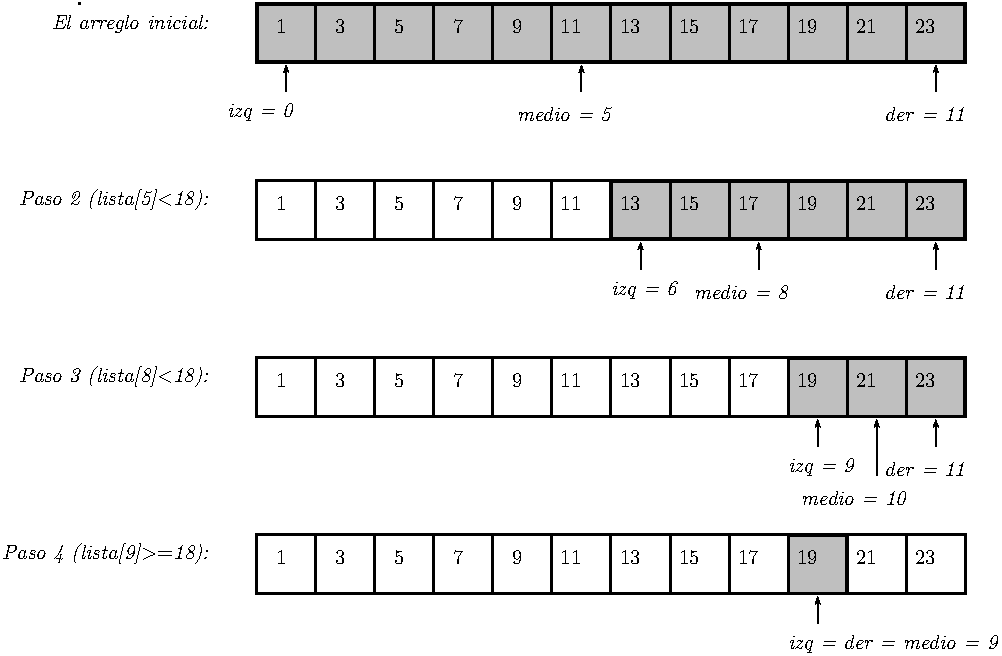
\includegraphics[width=\linewidth]{graficos/uni8-seguimiento}
\end{center}
\caption{Ejemplo de una búsqueda usando el algoritmo de búsqueda binaria.
Como no se encontró al valor buscado, devuelve $-1$.}
\label{fig:busqbin}
\end{figure}

En el Código~\ref{busquedabinaria} mostramos una posible implementación de
este algoritmo.

\begin{codigo}{busqueda\_binaria.py}{Función de búsqueda binaria}
\label{busquedabinaria}
\lstinputlisting{src/8_busqueda/busb.py}
\end{codigo}

A continuación varias ejecuciones de prueba:

\begin{codigo-python-sn}
>>> busqueda_binaria([1, 3, 5], 0)
[DEBUG] izq: 0 der: 2 medio: 1
[DEBUG] izq: 0 der: 0 medio: 0
-1
>>> busqueda_binaria([1, 3, 5], 1)
[DEBUG] izq: 0 der: 2 medio: 1
[DEBUG] izq: 0 der: 0 medio: 0
0
>>> busqueda_binaria([1, 3, 5], 2)
[DEBUG] izq: 0 der: 2 medio: 1
[DEBUG] izq: 0 der: 0 medio: 0
-1
>>> busqueda_binaria([1, 3, 5], 3)
[DEBUG] izq: 0 der: 2 medio: 1
1
>>> busqueda_binaria([1, 3, 5], 5)
[DEBUG] izq: 0 der: 2 medio: 1
[DEBUG] izq: 2 der: 2 medio: 2
2
>>> busqueda_binaria([1, 3, 5], 6)
[DEBUG] izq: 0 der: 2 medio: 1
[DEBUG] izq: 2 der: 2 medio: 2
-1
>>> busqueda_binaria([], 0)
-1
>>> busqueda_binaria([1], 1)
[DEBUG] izq: 0 der: 0 medio: 0
0
>>> busqueda_binaria([1], 3)
[DEBUG] izq: 0 der: 0 medio: 0
-1
\end{codigo-python-sn}

\ejercicioc{En la línea 13 de |busqueda_binaria.py| efectuamos la división usando el
operador |//| en lugar de |/|. ¿Qué sucedería si utilizáramos |/|?  }

\subsection*{¿Cuántas comparaciones hace este programa?}

Para responder esto pensemos en el peor caso, es decir, que se descartaron
varias veces partes del segmento para finalmente llegar a un segmento vacío y
el valor buscado no se encontraba en la lista.

En cada paso el segmento se divide por la mitad y se desecha una de esas
mitades, y en cada paso se hace una comparación con el valor buscado. Por lo
tanto, la cantidad de comparaciones que hacen con el valor buscado es
aproximadamente igual a la cantidad de pasos necesarios para llegar a un
segmento de tamaño 1.
Veamos el caso más sencillo para razonar, y supongamos que la longitud de la
lista es una potencia de 2, es decir \lstinline+len(lista)+~$= 2^k$:

\begin{itemize}
\item Luego del primer paso, el segmento a tratar es de tamaño $2^k$.
\item Luego del segundo paso, el segmento a tratar es de tamaño $2^{k-1}$.
\item Luego del tercer paso, el segmento a tratar es de tamaño $2^{k-2}$.

$\ldots$

\item Luego del paso $k$, el segmento a tratar es de tamaño $2^{k-k}=1$.
\end{itemize}

Por lo tanto este programa hace aproximadamente $k$ comparaciones con el valor
buscado cuando \lstinline+len(lista)+~$= 2^k$.
Pero si despejamos $k$ de la ecuación anterior, podemos ver que este programa
realiza aproximadamente $\log_2($\lstinline+len(lista)+$)$ comparaciones.

Cuando \lstinline+len(lista)+ no es una potencia de 2 el razonamiento es menos
prolijo, pero también vale que este programa realiza aproximadamente
$\log_2$(\lstinline+len(lista)+$)$ comparaciones.

\begin{observacion}
Vemos entonces que si \lstinline!lista! es una lista ordenada, la búsqueda binaria es
{\bf muchísimo} más eficiente que la búsqueda lineal.
\end{observacion}

Veamos un ejemplo para entender cuánto más eficiente es la búsqueda binaria.
Supongamos que tenemos una lista de un millón de elementos.

\begin{itemize}
\item El algoritmo de búsqueda lineal hará una cantidad de operaciones proporcional
a un millón; es decir que en el peor caso hará 1.000.000 de comparaciones, y en
un caso promedio, 500.000 comparaciones.
\item El algoritmo de búsqueda binaria hará como máximo $\log_2(1\,000\,000)$
comparaciones, o sea ¡no más que 20 comparaciones!.
\end{itemize}

\section{Resumen}

\begin{itemize}

\item La {\bf búsqueda} de un elemento en una secuencia es un
algoritmo básico pero importante. El problema que intenta resolver puede
plantearse de la siguiente manera: Dada una secuencia de valores y un
valor, devolver el índice del valor en la secuencia, si se encuentra, de no
encontrarse el valor en la secuencia señalizarlo apropiadamente.

\item Una de las formas de resolver el problema es mediante la {\bf
búsqueda lineal}, que consiste en ir revisando uno a uno los elementos de
la secuencia y comparándolos con el elemento a buscar.  Este algoritmo no
requiere que la secuencia se encuentre ordenada.

\item Cuando la secuencia sobre la que se quiere buscar está ordenada, se
puede utilizar el algoritmo de {\bf búsqueda binaria}.  Al estar ordenada
la secuencia, se puede desacartar en cada paso la mitad de los elementos,
quedando entonces con una eficiencia algorítmica relativa al
$log($\lstinline!len(secuencia)!$)$. Este algoritmo sólo tiene sentido
utilizarlo sobre una secuencia ordenada.

\item El análisis del comportamiento de un algoritmo puede ser muy engañoso
si se tiene en cuenta el mejor caso, por eso suele ser mucho más
ilustrativo tener en cuenta el {\bf peor caso}.  En algunos casos
particulares podrá ser útil tener en cuenta, además, el {\bf caso
promedio}.
\end{itemize}


\newpage
\section{Ejercicios}

\extractionlabel{guia}
\begin{ejercicio}
Escribir una función que reciba una lista desordenada y un elemento, que:
\begin{partes}
\item Busque todos los elementos coincidan con el pasado por parámetro y
devuelva la cantidad de coincidencias encontradas.
\item Busque la primera coincidencia del elemento en la lista y devuelva su
posición.
\item Utilizando la función anterior, busque todos los elementos que coincidan
con el pasado por parámetro y devuelva una lista con las posiciones.
\end{partes}
\end{ejercicio}


\extractionlabel{guia}
\begin{ejercicio}
Escribir una función que reciba una lista de números no ordenada, que:
\begin{partes}
\item Devuelva el valor máximo.
\item Devuelva una tupla que incluya el valor máximo y su posición.
\item ¿Qué sucede si los elementos son cadenas de caracteres?
\end{partes}
{\bf Nota:} no utilizar \verb!lista.sort()!
\end{ejercicio}


\extractionlabel{guia}
\begin{ejercicio}
{\bf Agenda simplificada} \\
Escribir una función que reciba una cadena a buscar y una lista de tuplas
(nombre\_completo, telefono), y busque dentro de la lista, todas las
entradas que contengan en el nombre completo la cadena recibida (puede
ser el nombre, el apellido o sólo una parte de cualquiera de ellos).
Debe devolver una lista con todas las tuplas encontradas.
\end{ejercicio}


\extractionlabel{guia}
\begin{ejercicio}
{\bf Sistema de facturación simplificado} \\
Se cuenta con una lista ordenada de productos, en la que uno consiste en
una tupla de (identificador, descripción, precio), y una lista de los
productos a facturar, en la que cada uno consiste en una tupla de
(identificador, cantidad). \\
Se desea generar una factura que incluya la cantidad, la descripción, el
precio unitario y el precio total de cada producto comprado, y al final
imprima el total general. \\
Escribir una función que reciba ambas listas e imprima por
pantalla la factura solicitada.
\end{ejercicio}


\extractionlabel{guia}
\begin{ejercicio}
Escribir una función que reciba una lista ordenada y un elemento. Si el
elemento se encuentra en la lista, debe encontrar su posición mediante
búsqueda binaria y devolverlo.  Si no se encuentra, debe agregarlo a la
lista en la posición correcta y devolver esa nueva posición. (No utilizar
\verb!lista.sort()!.)
\end{ejercicio}


\chapter{Diccionarios}

En esta unidad analizaremos otra estructura de datos importante: los diccionarios.
Su importancia radica no sólo en las grandes posibilidades que presentan
como estructuras para almacenar información, sino también en que, en
Python, son utilizados por el propio lenguaje para realizar diversas
operaciones y para almacenar información de otras estructuras.

\section{Qué es un diccionario}

Según Wikipedia, ``[u]n diccionario es una obra de consulta de
palabras y/o términos que se encuentran generalmente ordenados
alfabéticamente. De dicha compilación de palabras o términos se
proporciona su significado, etimología, ortografía y, en el caso
de ciertas lenguas fija su pronunciación y separación silábica.''


Al igual que los diccionarios a los que se refiere Wikipedia,
los diccionarios de Python son una colección de términos (llamados
\emph{claves}) asociados a un \emph{valor} determinado. A diferencia de los
diccionarios a los que se refiere Wikipedia, el orden en los diccionarios de
Python no es relevante.

Dicho de otra manera, un diccionario es una colección de pares $(clave,
valor)$. A diferencia de las listas y tuplas, en lugar de acceder a un valor
mediante un índice numérico, el acceso será a través de su clave, que puede
ser de diversos tipos.

\begin{figure}[hbt]
\begin{tikzpicture}[
    every node/.style={node font=\ttfamily},
]
    \node [] (k1) {"ar"};
    \node [below=0.5em of k1] (k2) {"es"};
    \node [below=0.5em of k2] (k3) {"tv"};
    \node [right=of k1] (v1) {"Argentina"};
    \node [right=of k2] (v2) {"España"};
    \node [right=of k3] (v3) {"Tuvalu"};
    \path [flecha] (k1) -- (v1);
    \path [flecha] (k2) -- (v2);
    \path [flecha] (k3) -- (v3);

    \node [fit=(k1) (k2) (k3)] (claves) {};
    \node [above=0cm of claves.north,anchor=south] (lclaves) {$claves$};

    \node [fit=(v1) (v2) (v3)] (valores) {};
    \node [above=0cm of valores.north,anchor=south] (lvalores) {$valores$};

    \node [bloque,fit=(claves) (lclaves) (valores) (lvalores)] (caja) {};
\end{tikzpicture}
\caption{Un diccionario cuyas claves son dominios de Internet (\emph{top level
    domains}) y cuyos valores son los países correspondientes.}
\end{figure}

Las claves son únicas dentro de un diccionario, es decir que no puede haber
un diccionario que tenga dos veces la misma clave. Si se asigna un valor a
una clave ya existente, se reemplaza el valor anterior.

No hay una forma directa de acceder a una clave a través de su valor, y
nada impide que un mismo valor se encuentre asignado a distintas claves.

Dado que el orden en los diccionarios no es relevante, dos diccionarios
se consideran iguales si contienen las mismas claves asociadas a los mismos
valores, incluso aunque los elementos hayan sido agregados en diferente orden.

Al igual que las listas, los diccionarios son mutables. Esto significa que
podemos agregar, quitar y modificar los elementos de un diccionario
posteriormente a su creación.

Cualquier valor de tipo inmutable puede ser clave de un diccionario:
cadenas, enteros, tuplas (con valores inmutables en sus miembros), etc.  No hay
restricciones para los valores que el diccionario puede contener, cualquier
tipo puede ser el valor: listas, cadenas, tuplas, otros diccionarios,
etc.

\begin{sabias_que}
En otros lenguajes de programación, a los diccionarios se los llama \emph{arreglos asociativos},
\emph{mapas} o \emph{tablas}.
\end{sabias_que}

\section{Utilizando diccionarios en Python}

De la misma forma que con listas, es posible definir un diccionario
directamente con los miembros que va a contener, o bien inicializar el
diccionario vacío y luego agregar los valores de a uno o de a muchos.

Para definirlo junto con los miembros que va a contener, se encierra el
listado de valores entre llaves, las parejas de clave y valor se separan
con comas, y la clave y el valor se separan con ':'.

\begin{codigo-python-sn}
dominios = {'ar': 'Argentina', 'es': 'España', 'tv': 'Tuvalu'}
\end{codigo-python-sn}

\begin{observacion}
En Python el tipo de dato asociado a los diccionarios se llama |dict|:

\begin{codigo-python-sn}
>>> type(punto)
<class 'dict'>
\end{codigo-python-sn}
\end{observacion}

Para declararlo vacío y luego ingresar los valores, se lo declara como un
par de llaves sin nada en medio, y luego se asignan valores directamente a
los índices.

\begin{codigo-python-sn}
materias = {}
materias["lunes"] = [6103, 7540]
materias["martes"] = [6201]
materias["miércoles"] = [6103, 7540]
materias["jueves"] = []
materias["viernes"] = [6201]
\end{codigo-python-sn}

Para acceder al valor asociado a una determinada clave, se lo hace
de la misma forma que con las listas, pero utilizando la clave
elegida en lugar del índice.

\begin{codigo-python-sn}
>>> materias["lunes"]
[6103, 7540]
\end{codigo-python-sn}

\begin{atencion}
El acceso por clave falla si se provee una clave que no está en el diccionario:

\begin{codigo-python-sn}
>>> materias["domingo"]
(^Traceback (most recent call last):
  File "<stdin>", line 1, in <module>
KeyError: 'domingo'^)
\end{codigo-python-sn}
\end{atencion}

El operador |in| nos permite preguntar si una clave se encuentra o no en el
diccionario:

\begin{codigo-python-sn}
>>> "lunes" in materias
True
>>> "domingo" in materias
False
\end{codigo-python-sn}

Además podemos utilizar la función \lstinline{get}, que recibe una
clave $k$ y un valor por omisión $v$, y devuelve el valor asociado a la clave
$k$, en caso de existir, o el valor $v$ en caso contrario.

\begin{codigo-python-sn}
>>> materias.get("lunes", [])
[6103, 7540]
>>> materias.get("domingo", [])
[]
\end{codigo-python-sn}

Existen diversas formas de iterar los elementos de un diccionario. Por ejemplo,
es posible iterar por sus claves y usar esas claves para acceder a los valores:

\begin{codigo-python-sn}
for dia in materias:
    print("El {} tengo que cursar {}".format(dia, materias[dia])
\end{codigo-python-sn}

Es posible, también, obtener los valores como tuplas donde el primer
elemento es la clave y el segundo el valor.

\begin{codigo-python-sn}
for dia, codigos in materias.items():
    print("El {} tengo que cursar {}".format(dia, codigos)
\end{codigo-python-sn}

Recordar que el orden de los elementos no es relevante; por lo tanto no podemos
asumir que el resultado de la iteración saldrá en ningún orden
particular\footnote{En versiones recientes de Python el orden de iteración
corresponde al orden en que los elementos fueron añadidos al diccionario; en
las versiones anteriores no se daba ninguna garantía acerca del orden de
iteración.}. Además, no es posible obtener porciones de un diccionario
usando \lstinline![:]!.

Hay muchas otras operaciones que se
pueden realizar sobre los diccionarios, que permiten manipular la información
según sean nuestras necesidades. Algunos de estos métodos pueden verse en
la referencia al final de la unidad.

\begin{sabias_que}
En la sección \ref{lookup-listas} mencionamos que Python garantiza que para
cualquier lista |L| con $N$ elementos se cumple que |L[i]| es una operación de
\emph{tiempo constante}, sin importar el valor de $N$ o de |i|.

Los diccionarios en Python tienen la misma propiedad: para cualquier
diccionario |D| con $N$ pares clave-valor, y para cualquier clave |k|, la
operación |D[k]| es de tiempo constante.

Dado que las claves pueden ser de cualquier tipo (a diferencia de las listas, en
las que los índices son números enteros entre 0 y $N-1$), para garantizar esta
propiedad, el algoritmo utilizado para almacenar los datos en el diccionario
debe ser más sofisticado que el utilizado para las listas.

Los diccionarios de Python están implementados usando una estructura de datos
llamada \emph{tabla de hash}. Para cada clave se calcula un valor numérico
mediante un algoritmo llamado \emph{código de hash}, que produce valores
muy dispares dependiendo de la clave.  Por ejemplo, el hash de la cadena
|"Python"| es -539294296 mientras que el de |"python"|, una cadena que
difiere en un caracter, es 1142331976. Los pares clave-valor del diccionario
se guardan internamente en una lista, y el código de hash de la clave se
utiliza para determinar el índice en la lista donde se ubicará cada par.
\end{sabias_que}

\section{Algunos usos de diccionarios}

Los diccionarios son una herramienta muy versátil.  Se puede utilizar un
diccionario, por ejemplo, para contar cuántas apariciones de cada palabra
hay en un texto, o cuántas apariciones de cada letra.

Es posible utilizar un diccionario, también, para tener una agenda donde la
clave es el nombre de la persona, y el valor es una lista con los datos
correspondientes a esa persona.

También podría utilizarse un diccionario para mantener los datos de los
alumnos inscriptos en una materia, siendo la clave el número de padrón, y
el valor una lista con todas las notas asociadas a ese alumno.

En general, los diccionarios sirven para crear bases de datos muy simples,
en las que la clave es el identificador del elemento, y el valor son todos
los datos del elemento a considerar.

Otro posible uso de un diccionario sería para realizar
traducciones, donde la clave sería la palabra en el idioma original y el
valor la palabra en el idioma al que se quiere traducir.  Sin embargo esta
aplicación es poco destacable, ya que esta forma de traducir suele dar
resultados poco satisfactorios.

\section{Resumen}

\begin{itemize}
\item Los diccionarios son una estructura de datos
muy poderosa, que permite almacenar un conjunto de pares $clave \rightarrow valor$.
\item Las claves deben ser inmutables y únicas.
\item Los valores pueden ser de cualquier tipo, y pueden no ser únicos.
\item El orden de los elementos no es relevante.
\end{itemize}

\begin{referencia_python}

\begin{sintaxis}{\lstinline!\{clave1:valor1, clave2:valor2\}!}
Se crea un nuevo diccionario con los valores asociados a las claves.  Si no
se ingresa ninguna pareja de clave y valor, se crea un diccionario vacío.
\end{sintaxis}

\begin{sintaxis}{\lstinline{diccionario[clave]}}
Accede al valor asociado con \lstinline!clave! en el diccionario. Falla si la
clave no está en el diccionario.
\end{sintaxis}

\begin{sintaxis}{\lstinline{clave in diccionario}}
Indica si un diccionario tiene o no una determinada clave.
\end{sintaxis}

\begin{sintaxis}{\lstinline{diccionario.get(clave, valor_predeterminado)}}
Devuelve el valor asociado a la clave.  A diferencia del acceso directo
utilizando \lstinline{[clave]}, en el caso en que el valor no se
encuentre devuelve el |valor_predeterminado|.
\end{sintaxis}

\begin{sintaxis}{\lstinline{for clave in diccionario:}}
Permite recorrer una a una todas las claves almacenadas en
el diccionario.
\end{sintaxis}

\begin{sintaxis}{\lstinline{diccionario.keys()}}
Devuelve una secuencia con todas las claves que se hayan ingresado
al diccionario.
\end{sintaxis}

\begin{sintaxis}{\lstinline{diccionario.values()}}
Devuelve una secuencia con todos los valores que se hayan
ingresado al diccionario.
\end{sintaxis}

\begin{sintaxis}{\lstinline{diccionario.items()}}
Devuelve una secuencia con tuplas de dos elementos, en las que el
primer elemento es la clave y el segundo el valor.
\end{sintaxis}

\begin{sintaxis}{\lstinline{diccionario.pop(clave)}}
Quita del diccionario la clave y su valor asociado, y devuelve el valor.
\end{sintaxis}
\end{referencia_python}


\newpage
\section{Ejercicios}

\extractionlabel{guia}
\begin{ejercicio}
Escribir una función que reciba una lista de tuplas, y que devuelva
un diccionario en donde las claves sean los primeros elementos de las
tuplas, y los valores una lista con los segundos.

Por ejemplo:
\begin{lstlisting}[numbers=none]
>>> l = [ ('Hola', 'don Pepito'), ('Hola', 'don Jose'),
          ('Buenos', 'días') ]
>>> print(tuplas_a_diccionario(l))
{ 'Hola': ['don Pepito', 'don Jose'], 'Buenos': ['días'] }
\end{lstlisting}
\end{ejercicio}

\extractionlabel{guia}
\begin{ejercicio}
{\bf Diccionarios usados para contar.}
\begin{partes}
  \item Escribir una función que reciba una cadena y devuelva un diccionario con
la cantidad de apariciones de cada palabra en la cadena.  Por ejemplo, si
recibe "Qué lindo día que hace hoy" debe devolver:
\lstinline!{ 'que': 2, 'lindo': 1, 'día': 1, 'hace': 1, 'hoy': 1}!.

  \item Escribir una función que cuente la cantidad de apariciones de cada
caracter en una cadena de texto, y los devuelva en un diccionario.

  \item Escribir una función que reciba una cantidad de iteraciones de una tirada
de 2 dados a realizar y devuelva la cantidad de veces que se observa cada valor
de la suma de los dos dados. \\
{\bf Nota}: utilizar el módulo \verb!random! para obtener tiradas aleatorias.
\end{partes}
\end{ejercicio}

\extractionlabel{guia}
\begin{ejercicio}
{\bf Continuación de la agenda.} \\
Escribir un programa que vaya solicitando al usuario que ingrese nombres.
\begin{partes}
  \item Si el nombre se encuentra en la agenda (\emph{implementada con un
diccionario}), debe mostrar el teléfono y, opcionalmente, permitir
modificarlo si no es correcto.
  \item Si el nombre no se encuentra, debe permitir ingresar el teléfono
correspondiente.
\end{partes}
El usuario puede utilizar la cadena "*", para salir del programa.
\end{ejercicio}

\extractionlabel{guia}
\begin{ejercicio}
Escribir una función que reciba un texto y para cada caracter presente en el
texto devuelva la cadena más larga en la que se encuentra ese caracter.
\end{ejercicio}

\newpage
\begin{subappendices}
\section{Conjuntos}

Supongamos que queremos modelar un registro de donantes de órganos.
Este registro se comporta como un \emph{conjunto} de elementos, donde cada
elemento es una persona, y el conjunto:

\begin{enumerate}
    \item no puede contener elementos repetidos: una persona puede ser donante
        o no, pero no puede figurar dos o más veces en el registro.
    \item debe permitir averiguar si un elemento pertenece o no al conjunto en
        \emph{tiempo constante}: no importa si hay 1, 10 o 100000 donantes,
        queremos tener la capacidad de averiguar si una persona determinada
        es donante o no rápidamente.
\end{enumerate}

Si implementáramos el registro usando una lista de Python, nos encontraríamos
con que no cumplimos con los requisitos:

\begin{enumerate}
    \item La lista puede contener elementos repetidos. Si bien podemos salvar este
        detalle preguntando si el elemento se encuentra o no en la lista antes
        de agregarlo, esto sería muy poco eficiente, ya que:
    \item Como vimos en la Sección~\ref{busqueda-lineal}, buscar un elemento en la
        lista consume una cantidad de tiempo proporcional a la cantidad de
        elementos presentes en la lista, con lo que no es posible cumplir con
        el requerimiento de tiempo constante.
\end{enumerate}

Una solución posible es usar un diccionario, guardando como clave el número de
documento de la persona donante, y como valor\ldots\ ¡cualquier cosa! No
importa qué vayamos asignar como valor, ya que lo único que queremos aprovechar
del diccionario es la capacidad de tener claves únicas y poder preguntar en
tiempo constante si una clave está o no presente. Por ejemplo, si usamos |True|
como valor:

\begin{codigo-python-sn}
>>> donantes = {12345: True, 23456: True}
>>> 23456 in donantes
True
>>> 34567 in donantes
False
>>> donantes.pop(23456)
>>> 23456 in donantes
False
\end{codigo-python-sn}

Sin embargo, utilizar un diccionario para modelar un conjunto de elementos no
es la solución más elegante. Hay una mejor forma de hacerlo, que es
utilizando el tipo de datos |set|\footnote{La palabra ``set'' significa
``conjunto'' en inglés.}.

Para crear un |set| usamos la sintaxis |{<expresión>, <expresión>, ...}|:

\begin{codigo-python-sn}
>>> donantes = {12345, 23456}
>>> type(donantes)
<class 'set'>
>>> 23456 in donantes
True
>>> 34567 in donantes
False
>>> donantes.remove(23456)
>>> 23456 in donantes
False
\end{codigo-python-sn}

Un |set| es una estructura de datos mutable (como las listas y los
diccionarios), que permite agregar y quitar elementos cumpliendo los requisitos de
unicidad y búsqueda en tiempo constante. Además es posible hacer operaciones
entre |set|s como unión, intersección y diferencia muy fácilmente:

\begin{codigo-python-sn}
>>> s1 = {1, 2, 3, 4}
>>> s1
{1, 2, 3, 4}
>>> s1.add(1)
>>> s1
{1, 2, 3, 4}
>>> s2 = {3, 4, 5, 6}
>>> s1.union(s2)
{1, 2, 3, 4, 5, 6}
>>> s1.intersection(s2)
{3, 4}
>>> s1.difference(s2)
{1, 2}
\end{codigo-python-sn}

Notar que la sintaxis para crear un conjunto es muy similar a la de creación de
diccionarios. El caso especial es cuando queremos crear un conjunto vacío: la
sintaxis |{}| no funcionará, ya que eso crea un diccionario vacío. Podemos
crear un conjunto vacío con: |set()|.

\begin{codigo-python-sn}
>>> type({})
<class 'dict'>
>>> type(set())
<class 'set'>
\end{codigo-python-sn}

La referencia completa del tipo de dato |set| puede verse en
\url{https://docs.python.org/3/library/stdtypes.html#set}.
\end{subappendices}

\chapter{Documentación, contratos y mutabilidad}

En esta unidad se le dará cierta formalización a algunos temas que habían sido
presentados informalmente, como por ejemplo la documentación de las funciones.

Se formalizarán las condiciones que debe cumplir un algoritmo al comenzar, en
su transcurso, y al terminar, y algunas técnicas para tener en cuenta estas
condiciones.

También se verá una forma de modelar el espacio donde \textit{viven} las
variables.

\section{Documentación}

Comenzamos formalizando un poco más acerca de la documentación, cuál es su
objetivo y las distintas formas de documentar.

\subsection{Comentarios vs documentación}

En Python tenemos dos convenciones diferentes para documentar nuestro código:
la \emph{documentación} propiamente dicha (lo que ponemos entre \verb|"| o
\verb|"""| al principio de cada función o módulo), y los \emph{comentarios}
(\verb|#|).  En la mayoría de los lenguajes de programación hay convenciones
similares. ¿Por qué tenemos dos formas diferentes de documentar?

La \emph{documentación} tiene como objetivo explicar \emph{qué} hace el código.
La documentación está dirigida a cualquier persona que desee utilizar la
función o módulo, para que pueda entender cómo usarla sin necesidad de leer el
código fuente.  Esto es útil incluso cuando quien implementó la función es la
misma persona que la va a utilizar, ya que permite separar responsabilidades.

Los \emph{comentarios} tienen como objetivo explicar \emph{cómo} funciona el
código, y \emph{por qué} se decidió implementarlo de esa manera. Los comentarios
están dirigidos a quien esté leyendo el código fuente.

Podemos ver la diferencia entre la documentación y los comentarios en la
función |elegir_codigo| de nuestra implementacion del juego Mastermind
(Código~\ref{cod:mastermind}):

\begin{codigo-python-sn}
def elegir_codigo():
    """Devuelve un codigo de 4 digitos elegido al azar"""
    digitos = ('0','1','2','3','4','5','6','7','8','9')
    codigo = ''
    for i in range(4):
        candidato = random.choice(digitos)
        # Debemos asegurarnos de no repetir digitos
        while candidato in codigo:
            candidato = random.choice(digitos)
        codigo = codigo + candidato
    return codigo
\end{codigo-python-sn}

\subsection{¿Por qué documentamos?}

Seamos sinceros: nadie quiere escribir documentación. ¿Para qué repetir con
palabras lo que ya está estipulado en el código? La documentación es algo que
muy a menudo se deja \emph{para después}, y cuando llega el tan angustioso
momento de escribirla, lo que se termina haciendo es escribir lo más
escueto posible que pueda pasar como ``documentación''.

Incluso es muy frecuente que durante el desarrollo de un proyecto el código
evolucione con el tiempo, pero que nos olvidemos de actualizar la documentación
para reflejar los cambios. En este caso no solamente tenemos documentación de
mala calidad, ¡sino que además es incorrecta!

Pese a todo esto, la realidad sigue siendo que una buena documentación es
componente esencial de cualquier proyecto exitoso. Esto en parte se debe a que
el código fuente transmite en detalle las operaciones individuales que componen
un algoritmo o programa, pero no suele transmitir en forma transparente cosas
como la \emph{intención} del programa, el \emph{diseño} de alto nivel, las
\emph{razones} por las que se decidió utilizar un algoritmo u otro, etc.

\subsection{Código autodocumentado}

En teoría, si nuestro código pudiera transmitir en forma eficiente todos esos
conceptos, la documentación sería menos necesaria. De hecho, existe una técnica de
programación llamada \emph{código autodocumentado}, en la que la idea principal
es elegir los nombres de funciones y variables de forma tal que la
documentación sea innecesaria.

Tomemos como ejemplo el siguiente código:

\begin{codigo-python-sn}
a = 9.81
b = 5
c = 0.5 * a * b**2
\end{codigo-python-sn}

Leyendo esas tres líneas de código podemos razonar cuál será el valor final de
las variables |a|, |b| y |c|, pero no hay nada que nos indique qué representan
esas variables, o cuál es la intención del código. Una opción para mejorarlo sería
utilizar comentarios para aclarar la intención:

\begin{codigo-python-sn}
a = 9.81   # Valor de la constante G (aceleración gravitacional), en m/s²
b = 5      # Tiempo en segundos
c = 0.5 * a * b**2  # Desplazamiento (en metros)
\end{codigo-python-sn}

Otra opción, según la técnica de código autodocumentado, es simplemente asignar
nombres descriptivos a las variables:

\begin{codigo-python-sn}
aceleracion_gravitacional = 9.81
tiempo_segundos = 5
desplazamiento_metros = 0.5 * aceleracion_gravitacional * tiempo_segundos ** 2
\end{codigo-python-sn}

De esta manera logramos que no sea necesario ningún comentario ni documentación
adicional, ya que la intención del código es mucho más descriptiva.

La técnica de código autodocumentado presenta varias limitaciones. Entre ellas:

\begin{itemize}
    \item Elegir buenos nombres es una tarea difícil, que
        requiere tener en cuenta cosas como: qué tan descriptivo es el nombre
        (cuanto más, mejor), la longitud del identificador
        (cuanto más corto mejor), el alcance del identificador (cuánto más
        grande, más descriptivo debe ser el nombre), y convenciones (|i| para
        índices, |c| para caracteres, etc).
    \item La documentación de todas formas termina siendo necesaria, ya que por
        muy bien que elijamos los nombres, muchas veces la única forma de
        explicar la intención del código y todos sus detalles es en lenguaje
        coloquial.
    \item En ciertos contextos sigue siendo deseable, o imprescindible, que
        quien quiera utilizar nuestra función o módulo pueda entender su
        funcionamiento sin necesidad de leer el código fuente.
\end{itemize}

\subsection{Un error común: la sobredocumentación}

Si bien la ausencia de documentación suele ser perjudicial, el otro extremo
también lo es: la \emph{sobredocumentación}. Después de todo, en la vida
diaria no necesitamos carteles que nos recuerden cosas como ``esta es la
puerta'', ``este es el picaporte'' y ``empujar hacia abajo para abrir''. De
la misma manera, podríamos decir que el siguiente código peca de ser sobredocumentado:

\begin{codigo-python-sn}
def buscar_elemento(lista_de_numeros, numero):
    """Esta función devuelve el índice (contando desde 0) en el que se
       encuentra el número `numero` en la lista `lista_de_numeros`.
       Si el elemento no está en la lista devuelve -1.
    """
    # Recorremos todos los índices de la lista, desde 0 (inclusive) hasta N
    # (no inclusive)
    for indice in range(len(lista_de_numeros)):
        # Si el elemento en la posicion `indice` es el buscado
        if lista_de_numeros[indice] == numero:
            # Devolvemos el índice en el que está el elemento
            return indice
    # No lo encontramos, devolvemos -1
    return -1
\end{codigo-python-sn}

Algunas cosas que podemos mejorar:

\begin{itemize}
\item En la firma de la función los nombres |buscar_elemento|,
    |lista_de_numeros| y |numero| se pueden simplificar a |buscar|, |secuencia| y
    |elemento|. Cambiamos |lista_de_numeros| por |secuencia|, ya que la función
    puede recibir secuencias de cualquier tipo, con elementos de cualquier
    tipo, y no hay ninguna razón para limitar a que sea una lista de números.
\item Las variable interna |indice| también se puede simplificar:
    por convención podemos usar |i|.
\item ``Esta función'' es redundante: cuando alguien lea la documentación ya va
    a saber que se trata de una función.
\item ``contando desde 0'' es redundante: en Python siempre contamos desde 0.
\item Los comentarios son excesivos: la función es suficientemente simple y
    cualquier persona que sepa programación básica podrá entender el algoritmo.
\end{itemize}

Corrigiendo todos estos detalles resulta:

\begin{codigo-python-sn}
def buscar(lista, elemento):
    """Devuelve el índice en el que se encuentra el `elemento` en la `lista`,
       o -1 si no está.
    """
    for i in range(len(lista)):
        if lista[i] == elemento:
            return i
    return -1
\end{codigo-python-sn}

\section{Contratos}

Cuando hablamos de \textit{contratos} o \textit{programación por
contratos}, nos referimos a la necesidad de estipular tanto lo que necesita
como lo que devuelve nuestro código. El contrato de una función suele ser
incluido en su documentación.

Algunos ejemplos de cosas que deben ser estipuladas como parte del contrato
son: cómo deben ser los parámetros recibidos, cómo va a ser lo que se devuelve,
y si la función provoca algún efecto secundario (como por ejemplo modificar
alguno de los parámetros recibidos o imprimir algo en la consola).

Algunas de estas condiciones deben estar dadas antes de ejecutar el código o
función; a estas condiciones las llamamos \emph{precondiciones}. Si se cumplen
las precondiciones, habrá un conjunto de condiciones sobre el estado en que
quedan las variables y el o los valores de retorno una vez finalizada la
ejecución, que llamamos \emph{postcondiciones}.

\subsection{Precondiciones}

Las precondiciones de una función son las condiciones que deben cumplirse antes
de ejecutarla, para que se comporte correctamente: cómo deben ser los
parámetros que recibe, cómo debe ser el estado global, etc.

Por ejemplo, en una función que divide dos números, las precondiciones son que los parámetros
son números, y que el divisor es distinto de 0.

Si estipulamos las precondiciones como parte de la documentación, en el cuerpo
de la función podremos asumir que son ciertas, y no será necesario escribir
código para lidiar con los casos en los que no se cumplen.

\subsection{Postcondiciones}

Las postcodiciones son las condiciones que se cumplirán una vez finalizada la
ejecución de la función (asumiendo que se cumplen las precondiciones): cómo
será el valor de retorno, si los parámetros recibidos o variables globales son
alteradas, si se imprimen cosas, si se modifican archivos, etc.

En el ejemplo anterior, la función división, dadas las precondiciones
puede asegurar que devolverá un número correspondiente al cociente solicitado.

\subsection{Aseveraciones}

Tanto las precondiciones como las postcondiciones son \textit{aseveraciones}
(en inglés \textit{assertions}). Es decir, afirmaciones realizadas en un momento
particular de la ejecución sobre el estado computacional. Si llegaran a ser
falsas significaría que hay algún error en el diseño o utilización del algoritmo.

En algunos casos puede ser útil comprobar estas afirmaciones desde el código, y
para ello podemos utilizar la instrucción \lstinline!assert!. Esta instrucción
recibe una condición a verificar (o sea, una expresión booleana).
Si la condición es |True|, la instrucción no hace nada; en caso contrario se
produce un error.

\begin{codigo-python-sn}
>>> assert True
>>> assert False
(^Traceback (most recent call last):
  File "<stdin>", line 1, in <module>
AssertionError^)
\end{codigo-python-sn}

Opcionalmente, la instrucción |assert| puede recibir
un mensaje de error que mostrará en caso que la condición no se cumpla.

\begin{codigo-python-sn}
>>> n = 0
>>> assert n != 0, "El divisor no puede ser 0"
(^Traceback (most recent call last):
  File "<stdin>", line 1, in <module>
AssertionError: El divisor no puede ser 0^)
\end{codigo-python-sn}

\begin{atencion}
Es importante tener en cuenta que \lstinline!assert! está pensado para ser
usado en la etapa de desarrollo. Un programa terminado nunca debería dejar
de funcionar por este tipo de errores.
\end{atencion}

\subsection{Ejemplos}

Usando los ejemplos anteriores, la función \lstinline!division! nos
quedaría de la siguiente forma:

\begin{codigo-python-sn}
def division(dividendo, divisor):
    """Cálculo de la división

    Pre: Recibe dos números, divisor debe ser distinto de 0.
    Post: Devuelve un número real, con el cociente de ambos.
    """
    assert divisor != 0, "El divisor no puede ser 0"
    return dividendo / divisor
\end{codigo-python-sn}

Otro ejemplo, tal vez más interesante, puede ser una función que implemente
una sumatoria ($\sum_{i=inicial}^{final} f(i)$).  En este caso hay que
analizar cuáles van a ser los parámetros que recibirá la función, y las
precondiciones que estos parámetros deberán cumplir.

La función |sumatoria| a escribir necesita de un valor inicial, un valor
final, y una función a la cual llamar en cada paso. Es decir que recibe
tres parámetros.

\begin{codigo-python-sn}
def sumatoria(inicial, final, f):
\end{codigo-python-sn}

Tanto \lstinline!inicial! como \lstinline!final! deben ser números enteros,
y dependiendo de la implementación a realizar o de la especificación
previa, puede ser necesario que \lstinline!final! deba ser mayor o igual a
\lstinline!inicial!.

Con respecto a \lstinline!f!, se trata de una función que será llamada con
un parámetro en cada paso y se requiere poder sumar el resultado, por lo
que debe ser una función que reciba un número y devuelva un número.

La declaración de la función queda, entonces, de la siguiente manera.

\begin{codigo-python-sn}
def sumatoria(inicial, final, f):
    """Calcula la sumatoria desde i=inicial hasta final de f(i)

    Pre: inicial y final son números enteros, f es una función que
         recibe un entero y devuelve un número.
    Post: Se devuelve el valor de la sumatoria de aplicar f a cada
          número comprendido entre inicial y final.
    """
\end{codigo-python-sn}

\begin{ejercicio}
Realizar la implementación correspondiente a la función \lstinline!sumatoria!.
\end{ejercicio}

En definitiva, la estipulación de pre y postcondiciones dentro de la
documentación de las funciones es una forma de especificar claramente el
comportamiento del código.  Las pre y postcondiciones son, en efecto, un
\textit{contrato} entre el código invocante y el invocado.

\section{Invariantes de ciclo}

% TODO: conseguir frase, la vida es siempre igual, siempre está cambiando.
%\begin{quote}
%``Dadme un punto de apoyo y moveré el mundo'' Arquímedes
%\end{quote}

\label{invariantes}
Los invariantes se refieren a estados o situaciones que no cambian dentro
de un contexto o porción de código.  Hay invariantes de ciclo, que son los
que veremos a continuación, e invariantes de estado, que se verán más
adelante.

El invariante de ciclo permite conocer cómo llegar desde las precondiciones
hasta las postcondiciones, cuando la implementación se compone de un ciclo.
El invariante de ciclo es, entonces, una
aseveración que debe ser verdadera al comienzo de cada iteración.

Por ejemplo, si el problema es ir desde el punto $A$ al punto $B$, las
precondiciones dicen que estamos parados en $A$ y las postcondiciones que
estamos parados en $B$, un invariante podría ser ``estamos en algún punto entre
$A$ y $B$, en el punto más cercano a $B$ que estuvimos hasta ahora.''.

Más específicamente, si analizamos el ciclo para buscar el máximo en una lista
desordenada, la precondición es que la lista contiene elementos que son
comparables y la postcondición es que se devuelve el elemento máximo de la
lista.

\begin{codigo-python-sn}
def maximo(lista):
    "Devuelve el elemento máximo de la lista o None si está vacía."
    if not lista:
        return None
    max_elem = lista[0]
    for elemento in lista:
        if elemento > max_elem:
            max_elem = elemento
    return max_elem
\end{codigo-python-sn}

En este caso, el invariante del ciclo es que \lstinline!max_elem! contiene el
valor máximo de la porción de lista analizada.

Los invariantes son de gran importancia al momento de demostrar que un
algoritmo funciona, pero aún cuando no hagamos una demostración formal es muy
útil tener los invariantes a la vista, ya que de esta forma es más fácil
entender cómo funciona un algoritmo y encontrar posibles errores.

Los invariantes, además, son útiles a la hora de determinar las condiciones
iniciales de un algoritmo, ya que también deben cumplirse para ese caso.  Por
ejemplo, consideremos el algoritmo para obtener la potencia \lstinline!n! de
un número.

\begin{codigo-python-sn}
def potencia(b, n):
    "Devuelve la potencia n del número b, con n entero mayor que 0."
    p = 1
    for i in range(n):
        p *= b
    return p
\end{codigo-python-sn}

En este caso, el invariante del ciclo es que la variable \lstinline!p!
contiene el valor de la potencia correspondiente a esa iteración. Teniendo en
cuenta esta condición, es fácil ver que \lstinline!p! debe comenzar el ciclo
con un valor de 1, ya que ese es el valor correspondiente a $p^0$.

De la misma manera, si la operación que se quiere realizar es sumar todos los
elementos de una lista, el invariante será que una variable \lstinline!suma!
contenga la suma de todos los elementos ya recorridos, por lo que es claro que
este invariante debe ser 0 cuando aún no se haya recorrido ningún elemento.

\begin{codigo-python-sn}
def suma(lista):
    "Devuelve la suma de todos los elementos de la lista."
    suma = 0
    for elemento in lista:
        suma += elemento
    return suma
\end{codigo-python-sn}

% TODO
% \subsection{Invariantes como medida de cuánto falta}

%Dependiendo del problema y las herramientas con las que contemos algunos
%invariantes se pueden medir retomando el ejemplo de ir de A a B, uno podría
%medir la distancia hasta B para esta, pero si para medir la distancia hay que ir hasta B
%y volver deja de tener sentido. O al estar buscando el mínimo en una
%secuencia, cómo hago para comprobar que paso a paso tengo el mínimo de la
%secuencia que ya recorrí sin usar

\subsection{Comprobación de invariantes desde el código}

Cuando la comprobación necesaria para saber si seguimos ``en camino'' es simple,
se la puede tener directamente dentro del código.  Evitando seguir avanzando
con el algoritmo si se produjo un error crítico.

Por ejemplo, en una búsqueda binaria, el elemento a buscar debe ser mayor que
el elemento inicial y menor que el elemento final, de no ser así, no tiene sentido
continuar con la búsqueda.  Es posible, entonces, agregar una instrucción
que compruebe esta condición y de no ser cierta realice alguna acción para
indicar el error, por ejemplo, utilizando la instrucción \lstinline!assert!,
vista anteriormente.

\section{Mutabilidad e Inmutabilidad}
\label{mutabilidad}

Hasta ahora cada vez que estudiamos un tipo de datos indicamos si son
mutables o inmutables.

Cuando un valor es de un tipo inmutable, como por ejemplo una cadena, es
posible asignar un nuevo valor a esa variable, pero no es posible modificar su
contenido.

\begin{codigo-python-sn}
>>> s = "ejemplo"
>>> s = "otro"
>>> s[2] = "c"
(^Traceback (most recent call last):
  File "<stdin>", line 1, in <module>
TypeError: 'str' object does not support item assignment^)
\end{codigo-python-sn}

Esto se debe a que cuando se realiza una nueva asignación, no se modifica la
cadena en sí, sino que la variable \lstinline!s! pasa a \emph{referenciar} a otra cadena.
En cambio, no es posible asignar un nuevo caracter en una posición, ya que
esto implicaría modificar la cadena inmutable.

En el caso de los parámetros mutables, la asignación tiene el mismo
comportamiento, es decir que las variables pasan a apuntar a un nuevo valor.

\begin{codigo-python-sn}
>>> lista1 = [10, 20, 30]
>>> lista2 = lista1
>>> lista1 = [3, 5, 7]
>>> lista1
[3, 5, 7]
>>> lista2
[10, 20, 30]
\end{codigo-python-sn}

Algo importante a tener en cuenta en el caso de las variables de tipo
mutable es que si hay dos o más variables que \textit{referencian} a un mismo
valor, y este valor se modifica, el cambio se verá reflejado en ambas variables.

\begin{codigo-python-sn}
>>> lista1 = [1, 2, 3]
>>> lista2 = lista1
>>> lista2[1] = 5
>>> lista1
[1, 5, 3]
\end{codigo-python-sn}

\begin{sabias_que}
En otros lenguajes, como C o C++, existe un tipo de variable especial
llamado \emph{puntero}, que se comporta como una referencia a un valor,
como es el caso de las variables mutables del ejemplo anterior.

En Python no hay punteros como los de C o C++, pero todas las variables son
referencias a una porción de memoria, de modo que cuando se asigna una
variable a otra, lo que se está asignando es la porción de memoria a la que
refieren.  Si esa porción de memoria cambia, el cambio se puede ver en
todas las variables que apuntan a esa porción.
\end{sabias_que}

% TODO: describir en más detalle el modelo de referencia de python ?

\subsection{Parámetros mutables e inmutables}

Las funciones reciben parámetros que pueden ser mutables o inmutables.

Si dentro del cuerpo de la función se modifica uno de estos parámetros para
que \textit{referencie} a otro valor, este cambio no se verá reflejado fuera de la
función.  Si, en cambio, se modifica el \textit{contenido} de alguno de los
parámetros mutables, este cambio \textit{sí} se verá reflejado fuera de la
función.

A continuación un ejemplo en el cual se asigna la variable recibida, a un
nuevo valor.  Esa asignación sólo tiene efecto dentro de la función.

\begin{codigo-python-sn}
>>> def no_cambia_lista(lista):
...     lista = [0, 1, 2, 3]
...     print("Dentro de la funcion lista =", lista)
...
>>> lista = [10, 20, 30, 40]
>>> no_cambia_lista(lista)
Dentro de la funcion lista = [0, 1, 2, 3]
>>> lista
[10, 20, 30, 40]
\end{codigo-python-sn}

A continuación un ejemplo en el cual se modifica la variable recibida. En este
caso, los cambios realizados tienen efecto tanto dentro como fuera de la
función.

\begin{codigo-python-sn}
>>> def cambia_lista(lista):
...     for i in range(len(lista)):
...         lista[i] = lista[i] ** 3
...
>>> lista = [1, 2, 3, 4]
>>> cambia_lista(lista)
>>> lista
[1, 8, 27, 64]
\end{codigo-python-sn}

\begin{atencion}
Por omisión se espera que una función que recibe parámetros mutables no los
modifique, ya que si se los modifica se podría perder información valiosa.

En el caso en que por una decisión de diseño o especificación se modifiquen
los parámetros mutables recibidos, esto debe estar claramente documentado
como parte de las postcondiciones.
\end{atencion}

\section{Resumen}

\begin{itemize}
\item La \textbf{documentación} tiene como objetivo explicar \emph{qué} hace el código,
    y está dirigida a quien desee utilizar la función o módulo.
\item Los \textbf{comentarios} tienen como objetivo explicar \emph{cómo} funciona el
    código y \emph{por qué} se decidió implementarlo de esa manera, y están dirigidos a
    quien esté leyendo el código fuente.
\item El \textbf{contrato} de una función especifica qué condiciones se deben
    cumplir para que la función pueda ser invocada (\textbf{precondiciones}),
    y qué condiciones se garantiza que serán válidas cuando la función termine
    su ejecución (\textbf{postcondiciones}).
\item Los \textbf{invariantes de ciclo} son las condiciones que deben
cumplirse al comienzo de cada iteración de un ciclo.
\item En el caso en que estas \textbf{aseveraciones} no sean verdaderas, se
deberá a un error en el diseño o utilización del código.
\item Si una función modifica un valor mutable que recibe por parámetro, eso
    debe estar explícitamente aclarado en su documentación.
\end{itemize}

\begin{referencia_python}

\begin{sintaxis}{Documentación: \lstinline|"..."| ó \lstinline|"""..."""|}
    Por convención, si la primera línea de una función o módulo es una cadena,
    esa será su documentación
\end{sintaxis}

\begin{sintaxis}{Comentarios: \lstinline|# ...|}
    El intérprete ignora cualquier texto que se encuentra desde el caracter
    |#| hasta el fin de la línea.
\end{sintaxis}

\begin{sintaxis}{\lstinline!assert condicion[, mensaje]!}
Verifica si la condición es verdadera.  En caso contrario, provoca un error
con el mensaje recibido por parámetro.
\end{sintaxis}

\end{referencia_python}

\newpage
\section{Ejercicios}

\extractionlabel{guia}
\begin{ejercicio}
Analizar cada una de las siguientes funciones.
¿Cuál es el contrato de la función? ¿Cómo sería su documentación?
¿Es necesario agregar comentarios?
¿Se puede simplificar el código y/o mejorar su legibilidad?
¿Hay algún invariante de ciclo?

\begin{partes}

\item
\begin{minipage}{0.95\linewidth}
\begin{lstlisting}[numbers=none]
def Abs(i):
    if i >= 0:
        return i
    else:
        return -i
\end{lstlisting}
\end{minipage}

\item
\begin{minipage}{0.95\linewidth}
\begin{lstlisting}[numbers=none]
def emails(diccionario):
    for k, v in diccionario.items():
        print(f"El e-mail de {k} es {v}")
\end{lstlisting}
\end{minipage}

\item
\begin{minipage}{0.95\linewidth}
\begin{lstlisting}[numbers=none]
def emails2(diccionario):
    buenos = {}
    for k, v in diccionario.items():
        if '@' in v:
            buenos[k] = v
    return buenos
\end{lstlisting}
\end{minipage}

\item
\begin{minipage}{0.95\linewidth}
\begin{lstlisting}[numbers=none]
def emails3(nombres, direcciones):
    for nom in range(len(nombres)):
        if direcciones[nom] == None:
            nombre, apellido = ' '.split(nombres[nom].lower())
            direcciones[nom] = nombre[0] + apellido + '@ejemplo.com'
\end{lstlisting}
\end{minipage}

\end{partes}
\end{ejercicio}

\newpage
\begin{subappendices}
\section{Acertijo MU}

El acertijo MU\footnote{%
\url{http://en.wikipedia.org/wiki/Invariant\_(computer\_science)}} es un buen
ejemplo de un problema lógico donde es útil determinar el invariante.  El
acertijo consiste en buscar si es posible convertir MI a MU, utilizando las
siguientes operaciones.

\begin{enumerate}
\item Si una cadena termina con una I, se le puede agregar una U (xI -> xIU)
\item Cualquier cadena luego de una M puede ser totalmente duplicada (Mx ->
Mxx)
\item Donde haya tres Is consecutivas (III) se las puede reemplazar por una U
(xIIIy -> xUy)
\item Dos Us consecutivas, pueden ser eliminadas (xUUy -> xy)
\end{enumerate}

Para resolver este problema, es posible pasar horas aplicando estas reglas
a distintas cadenas.  Sin embargo, puede ser más fácil encontrar una
afirmación que sea invariante para todas las reglas y que muestre si es o
no posible llegar a obtener MU.

Al analizar las reglas, la forma de deshacerse de las Is es conseguir tener
tres Is consecutivas en la cadena.  La única forma de deshacerse de todas las
Is es que haya un cantidad de Is consecutivas múltiplo de tres.

Es por esto que es interesante considerar la siguiente afirmación como
invariante: el número de Is en la cadena no es múltiplo de tres.

Para que esta afirmación sea invariante al acertijo, para
cada una de las reglas se debe cumplir que: si el invariante era verdadero
antes de aplicar la regla, seguirá siendo verdadero luego de aplicarla.

Para ver si esto es cierto o no, es necesario considerar la aplicación del
invariante para cada una de las reglas.

\begin{enumerate}
\item Se agrega una U, la cantidad de Is no varía, por lo cual se mantiene el
invariante.
\item Se duplica toda la cadena luego de la M, siendo $n$ la cantidad de
Is antes de la duplicación, si $n$ no es múltiplo de 3, $2n$ tampoco lo será.
\item Se reemplazan tres Is por una U.  Al igual que antes, siendo $n$ la
cantidad de Is antes del reemplazo, si $n$ no es múltiplo de 3, $n-3$ tampoco
lo será.
\item Se eliminan Us, la cantidad de Is no varía, por lo cual se mantiene el
invariante.
\end{enumerate}

Todo esto indica claramente que el invariante se mantiene para cada una de las
posibles transformaciones.  Esto significa que sea cual fuere la regla que se
elija, si la cantidad de Is no es un múltiplo de tres antes de aplicarla, no
lo será luego de hacerlo.

Teniendo en cuenta que hay una única I en la cadena inicial MI, y que uno no
es múltiplo de tres, es imposible llegar a MU con estas reglas, ya que MU
tiene cero Is, que sí es múltiplo de tres.
\end{subappendices}

% TODO: temas que faltan:
% - acceso secuencial y aleatorio, (para la siguiente unidad: datos de tamaño
% fijo, indice)
% - entrada y salida estandard y estandard error

% TODO importante (errores vistos en los alumnos)
%  1) Mostrar ejemplos de lecturas que NO sean csv
%  2) Mostrar uso de csv como for linea in archivo

\chapter{Manejo de archivos}
\label{uni:archivos}

Veremos en esta unidad cómo manejar archivos desde nuestros
programas.

Existen dos formas básicas de acceder a un archivo, una es
utilizarlo como un archivo de texto, que procesaremos línea por
línea; la otra es tratarlo como un archivo binario, que
procesaremos byte por byte.

En Python, para abrir un archivo usaremos la función \lstinline!open!, que
recibe el nombre del archivo a abrir.

\begin{codigo-python-sn}
archivo = open("archivo.txt")
\end{codigo-python-sn}

Esta función intentará abrir el archivo con el nombre indicado.  Si tiene
éxito devolverá un valor de un tipo especial, que nos permitirá manipular el
archivo de diversas maneras.

La operación más sencilla a realizar sobre un archivo es leer su contenido.
Para procesarlo línea por línea, es posible hacerlo de la siguiente forma:

\begin{codigo-python-sn}
linea = archivo.readline()
while linea != '':
    # procesar linea
    linea = archivo.readline()
\end{codigo-python-sn}

Esto funciona ya que cada archivo que se encuentre abierto tiene una
posición asociada, que indica el último punto que fue leído.  Cada vez que
se lee una línea, avanza esa posición. Es por ello que
\lstinline!readline()! devuelve cada vez una línea distinta y no siempre la
misma.

La siguiente estructura es una forma equivalente a la vista en el ejemplo
anterior.

\begin{codigo-python-sn}
for linea in archivo:
    # procesar linea
\end{codigo-python-sn}

De esta manera, la variable \lstinline!linea! irá almacenando distintas cadenas
correspondientes a cada una de las líneas del archivo.

Es posible, además, obtener todas las líneas del archivo utilizando una
sola llamada a función:

\begin{codigo-python-sn}
lineas = archivo.readlines()
\end{codigo-python-sn}

En este caso, la variable \lstinline!lineas! tendrá una lista de cadenas con
todas las líneas del archivo.

\begin{atencion}
Es importante tener en cuenta que cuando se utilizan funciones como
\lstinline!archivo.readlines()!, se está cargando en memoria
el archivo completo.  Siempre que una instrucción cargue un archivo
completo en memoria debe tenerse cuidado de utilizarla sólo con archivos
pequeños, ya que de otro modo podría agotarse la memoria de la computadora.
\end{atencion}

\section{Cerrar un archivo}

Al terminar de trabajar con un archivo, es importante cerrarlo,
por diversos motivos: en algunos sistemas los archivos sólo pueden
ser abiertos de a un programa por la vez; en otros, lo que se haya
escrito no se guardará realmente hasta no cerrar el archivo; o el
límite de cantidad de archivos que puede manejar un programa puede
ser bajo, etc.

Para cerrar un archivo simplemente se debe llamar a:

\begin{codigo-python-sn}
archivo.close()
\end{codigo-python-sn}

Además, Python nos provee con una estructura que permite cerrar el archivo
automáticamente, sin necesidad de llamar a |close|:

\begin{codigo-python-sn}
with open("archivo.txt") as archivo:
    #
    # procesar el archivo
    #

# Cuando la ejecución sale del bloque 'with',
# el archivo se cierra automáticamente.
\end{codigo-python-sn}

\section{Ejemplo de procesamiento de archivos}

Por ejemplo, para mostrar todas las líneas de un archivo,
precedidas por el número de línea, podemos hacerlo de la siguiente manera:

\begin{codigo-python-sn}
archivo = open("archivo.txt")
i = 1
for linea in archivo:
    linea = linea.rstrip("\n")
    print("{}: {}".format(i, linea))
    i += 1
archivo.close()
\end{codigo-python-sn}

La llamada a \lstinline!rstrip! es necesaria ya que cada línea que se lee del
archivo contiene un caracter especial llamado {\it fin de línea} y con la llamada a
\lstinline!rstrip("\n")! se remueve.

Notar que sería equivalente usar el bloque |with| para ahorrarnos la llamada a
|close|:

\begin{codigo-python-sn}
(@with open("archivo.txt") as archivo:@)
    i = 1
    for linea in archivo:
        linea = linea.rstrip("\n")
        print("{}: {}".format(i, linea))
        i += 1
\end{codigo-python-sn}

\begin{sabias_que}
Los archivos de texto son sencillos de manejar, pero existen por lo menos 3
formas distintas de marcar un fin de línea. En Unix tradicionalmente se usa
el caracter '\verb!\n!' (valor de ASCII 10, definido como nueva línea) para
el fin de línea, mientras que en OSX el fin de línea se solía
representar como un '\verb!\r!' (valor ASCII 13, definido como retorno de
carro) y en Windows se usan ambos caracteres '\verb!\r\n!'.

Si bien esto es algo que hay que tener en cuenta en una diversidad de
casos, en particular en Python por omisión se maneja cualquier tipo de fin
de línea como si fuese un '\verb!\n!', salvo que se le pida lo contrario.
Para manejar los caracteres de fin de línea \textit{a mano} se puede poner
una 'U' en el parámetro modo que le pasamos a \lstinline!open!.
\end{sabias_que}

También podemos utilizar la función |enumerate| (explicada en la sección
\ref{enumerate}) para no tener que mantener el
contador |i| a mano:

\begin{codigo-python-sn}
with open("archivo.txt") as archivo:
    (@for i, linea in enumerate(archivo):@)
        linea = linea.rstrip("\n")
        print("{}: {}".format(i, linea))
\end{codigo-python-sn}

\section{Modo de apertura de los archivos}

La función \lstinline!open! recibe un parámetro opcional para indicar el
modo en que se abrirá el archivo.  Los tres modos de apertura que se pueden
especificar son:

\begin{itemize}
\item Modo de \textbf{sólo lectura} (\lstinline!'r'!).   En este caso no es
posible realizar modificaciones sobre el archivo, solamente leer su
contenido.

\item Modo de \textbf{sólo escritura} (\lstinline!'w'!). En este caso el
archivo es truncado (vaciado) si existe, y se lo crea si no existe.

\item Modo \textbf{sólo escritura posicionándose al final del archivo}
(\lstinline!a!). En este caso se crea el archivo, si no existe, pero en
caso de que exista se posiciona al final, manteniendo el contenido
original.

\end{itemize}

Por otro lado, en cualquiera de estos modos se puede agregar un
\lstinline!+! para pasar a un modo lectura-escritura. El comportamiento de
\lstinline!r+! y de \lstinline!w+! no es el mismo, ya que en el primer caso
se tiene el archivo completo, y en el segundo caso se trunca el archivo,
perdiendo así los datos.

\begin{observacion}
Si un archivo no existe y se lo intenta abrir en modo lectura, se generará
un error; en cambio si se lo abre para escritura, Python se encargará de
crear el archivo al momento de abrirlo, ya sea con \lstinline!'w'!,
\lstinline!'a'!, \lstinline!'w+'! o con \lstinline!'a+')!.
\end{observacion}

En caso de que no se especifique el modo, los archivos serán abiertos en
modo sólo lectura (\lstinline!r!).

\begin{atencion}
Si un archivo existente se abre en modo escritura (\lstinline!'w'! o
\lstinline!'w+'!), todos los datos anteriores son borrados y reemplazados
por lo que se escriba en él.
\end{atencion}

\section{Escribir en un archivo}

De la misma forma que para la lectura, existen dos formas distintas de
escribir a un archivo.  Mediante cadenas:

\begin{codigo-python-sn}
archivo.write(cadena)
\end{codigo-python-sn}

O mediante listas de cadenas:

\begin{codigo-python-sn}
archivo.writelines(lista_de_cadenas)
\end{codigo-python-sn}

Así como la función \lstinline!readline! devuelve las líneas con los caracteres
de fin de línea (\lstinline!\n!), será necesario agregar los caracteres de
fin de línea a las cadenas que se vayan a escribir en el archivo.

Por ejemplo, el siguiente programa genera a su vez el código de otro programa
Python y lo guarda en el archivo |saludo.py|:

\begin{codigo-python-sn}
with open("saludo.py", "w") as saludo:
    saludo.write("# Este programa fue generado por otro programa!\n")
    saludo.write("print 'Hola Mundo'\n")
\end{codigo-python-sn}

\begin{atencion}
Si un archivo existente se abre en modo lectura-escritura, al escribir en
él se sobreescribirán los datos anteriores, a menos que se haya llegado al
final del archivo.

Este proceso de sobreescritura se realiza caracter por caracter, sin
consideraciones adicionales para los caracteres de fin de línea ni otros
caracteres especiales.
\end{atencion}

\section{Agregar información a un archivo}

Abrir un archivo en modo {\it agregar al final} puede parece raro,
pero es bastante útil.

Uno de sus usos es para escribir un archivo de bitácora (o archivo de
{\textit log}), que nos permita ver los distintos eventos que se fueron
sucediendo, y así encontrar la secuencia de pasos (no siempre evidente) que
hace nuestro programa.

Esta es una forma muy habitual de buscar problemas o hacer un seguimiento
de los sucesos. Para los administradores de sistemas es una herramienta
esencial de trabajo.

En el Código \ref{modulo_log} se muestra un módulo para manejo de logs, que
se encarga de la apertura del archivo, del guardado de las líneas una por
una y del cerrado final del archivo.

\begin{codigo}{log.py}{Módulo para manipulación de archivos de log}
\label{modulo_log}
\lstinputlisting{src/11_archivos/log.py}
\end{codigo}

En este módulo se utiliza el módulo de Python \lstinline!datetime! para
obtener la fecha y hora actual que se guardará en los archivos.  Es
importante notar que en el módulo mostrado no se abre o cierra un archivo
en particular, sino que las funciones están programadas de modo tal que
puedan ser utilizadas desde otro programa.

Se trata de un módulo genérico que podrá ser utilizado por diversos programas,
que requieran la funcionalidad de registrar los posibles errores o eventos que
se produzcan durante la ejecución.

Para utilizar este módulo, será necesario primero llamar a
\lstinline!abrir_log! para abrir el archivo de log, luego llamar a
\lstinline!guardar_log! por cada mensaje que se quiera registrar, y
finalmente llamar a \lstinline!cerrar_log! cuando se quiera concluir la
registración de mensajes:

\begin{codigo-python-sn}
import log

ARCHIVO_LOG = "mi_log.txt"

archivo_log = log.abrir_log(ARCHIVO_LOG)
# ...
# Hacer cosas que pueden dar error
if error:
    guardar_log(archivo_log, "ERROR: " + error)
# ...
# Finalmente cerrar el archivo
log.cerrar_log(archivo_log)
\end{codigo-python-sn}

Este código, que incluye el módulo \lstinline!log! mostrado anteriormente,
muestra una forma básica de utilizar un archivo de log.  Al iniciarse el
programa se abre el archivo de log, de forma que queda registrada la fecha
y hora de inicio.  Posteriormente se realizan tareas varias que podrían
provocar errores, y de haber algún error se lo guarda en el archivo de log.
Finalmente, al terminar el programa, se cierra el archivo de log, quedando
registrada la fecha y hora de finalización.

El archivo de log generado tendrá la forma:

\begin{codigo-nohl-sn}
2016-04-10 15:20:32.229556 Iniciando registro de errores
2016-04-10 15:20:50.721415 ERROR: no se pudo acceder al recurso
2016-04-10 15:21:58.625432 ERROR: formato de entrada inválido
2016-04-10 15:22:10.109376 Fin del registro de errores
\end{codigo-nohl-sn}

\section{Manipular un archivo en forma binaria}

No todos los archivos son archivos de texto, y por lo tanto no todos los
archivos pueden ser procesados por líneas. Existen archivos en los que cada
byte tiene un significado particular, y es necesario manipularlos conociendo
el formato en que están los datos para poder procesar esa información.

Para abrir un archivo y manejarlo de forma binaria es necesario agregarle
una \verb!'b'! al parametro de modo:

\begin{codigo-python-sn}
archivo_binario = open('imagen.jpg', 'rb')
\end{codigo-python-sn}

\begin{sabias_que}
La \texttt{b} en el modo de apertura viene de \textit{binario}, por el
sistema de numeración binaria, ya que en el procesador de la computadora la
información es manejada únicamente mediante ceros o unos (bits) que
conforman números binarios.

Si bien no es necesaria en todos los sistemas (en general el mismo sistema
detecta que es un archivo binario sin que se lo pidamos), es una buena
costumbre usarla, por más que sirva principalmente como documentación.
\end{sabias_que}

Para procesar el archivo de a bytes en lugar de líneas, se utiliza la
función \lstinline!contenido = archivo.read(n)! para leer \lstinline!n!
bytes y \lstinline!archivo.write(contenido)!, para
escribir \lstinline!contenido! en la posición actual del archivo.

Al manejar un archivo binario, es necesario poder conocer la
posición actual en el archivo y poder modificarla. Para obtener la
posición actual se utiliza \lstinline!archivo.tell()!, que
indica la cantidad de bytes desde el comienzo del archivo.

Para modificar la posición actual se utiliza
\lstinline!archivo.seek(posicion)!, que permite desplazarse hacia el byte
ubicado en la posición indicada.

\begin{codigo-python-sn}
>>> f = open('imagen.jpg', 'rb')
>>> f.tell()
0
>>> datos = f.read(3)
>>> datos
b'\xff\xd8\xff'
>>> type(datos)
<class 'bytes'>
>>> f.tell()
3
>>> f.seek(0)
0
>>> datos = f.read()
>>> len(datos)
3150
\end{codigo-python-sn}

\begin{atencion}
Al trabajar con archivos binarios, la función |read| no devuelve cadenas de
caracteres (|str|), sino que devuelve una {\it secuencia de bytes} (|bytes|).
Análogamente, la función |write| recibe una secuencia de bytes.
\end{atencion}

\section{Persistencia de datos}

Se llama {\bf persistencia} a la capacidad de guardar la
información de un programa para poder volver a utilizarla en otro
momento. Es lo que los usuarios conocen como {\it Guardar el archivo}
y después {\it Abrir el archivo}. Pero para un programador puede
significar más cosas y suele involucrar un proceso de {\it
serialización} de los datos a un archivo o a una base de datos o a
algún otro medio similar, y el proceso inverso de recuperar los
datos a partir de la información {\it serializada}.

% Ejemplo Highscores

Por ejemplo, supongamos que en el desarrollo de un juego se quiere guardar
en un archivo la información referente a los ganadores, el puntaje máximo
obtenido y el tiempo de juego en el que obtuvieron ese puntaje.

En el juego, esa información podría estar almacenada en una lista de
tuplas:
\begin{codigo-python-sn}
[(nombre1, puntaje1, tiempo1), (nombre2, puntaje2, tiempo2), ...]
\end{codigo-python-sn}

Esta información se puede guardar en un archivo de muchas formas distintas.
En este caso, para facilitar la lectura del archivo de puntajes para los
humanos, se decide guardarlos en un archivo de texto, donde cada tupla
ocupará una línea y los valores de las tuplas estarán separados por
comas.

En el Código \ref{puntajes} se muestra un módulo capaz de guardar y
recuperar los puntajes en el formato especificado.

\begin{codigo}{puntajes.py}{Módulo para guardar y recuperar puntajes en un archivo}
\label{puntajes}
\lstinputlisting{src/11_archivos/puntajes.py}
\end{codigo}

Dadas las especificaciones del problema al guardar los valores en el
archivo, es necesario convertir el puntaje (que es un valor numérico) en
una cadena, y al abrir el archivo es necesario convertirlo nuevamente en un
valor numérico.

\begin{observacion}
Es importante notar que tanto la función que almacena los datos como la que
los recupera requieren que la información se encuentre de una forma
determinada y de no ser así, fallarán.  Es por eso que estas condiciones se
indican en la documentación de las funciones como sus precondiciones. En
próximas unidades veremos cómo evitar que falle una función si alguna de
sus condiciones no se cumple.
\end{observacion}

Es bastate sencillo probar el módulo programado y ver que lo que se guarda
es igual que lo que se recupera:

\begin{codigo-python-sn}
>>> import puntajes
>>> valores = [("Pepe", 108, "4:16"), ("Juana", 2315, "8:42")]
>>> puntajes.guardar_puntajes("puntajes.txt", valores)
>>> recuperado = puntajes.recuperar_puntajes("puntajes.txt")
>>> print recuperado
[('Pepe', 108, '4:16'), ('Juana', 2315, '8:42')]
\end{codigo-python-sn}

% Fin ejemplo.

Guardar el estado de un programa se puede hacer tanto en un
archivo de texto, como en un archivo binario. En muchas
situaciones es preferible guardar la información en un archivo de
texto, ya que de esta manera es posible modificarlo fácilmente
desde cualquier editor de textos.

En general, los archivos de texto consumen más
espacio, pero son más faciles de entender y fáciles de usar desde
cualquier programa.

Por otro lado, en un archivo binario bien definido se puede evitar el
desperdicio de espacio, o también hacer que sea más eficiente acceder a los
datos.

En definitiva, la decisión de qué formato usar queda a discreción del
programador. Es importante recordar que el sentido común es el valor más
preciado en un programador.

\subsection{Persistencia en archivos CSV}

Un formato que suele usarse para transferir datos entre programas es
\textbf{csv} (del inglés {\it comma separated values}: valores separados
por comas) es un formato bastante sencillo, tanto para leerlo como para
procesarlo desde el código, se parece al formato visto en el ejemplo
anteriormente.

\begin{codigo-nohl-sn}
Nombre,Apellido,Telefono,Cumpleaños
"John","Smith","555-0101","1973-11-24"
"Jane","Smith","555-0101","1975-06-12"
\end{codigo-nohl-sn}

En el ejemplo se puede ver una pequeña base de datos. En la primera línea
del archivo tenemos los nombres de los campos, un dato opcional desde el
punto de vista del procesamiento de la información, pero que facilita
entender el archivo.

En las siguientes lineas se ingresan los datos de la base de datos, cada
campo separado por comas. Los campos que son cadenas se suelen escribir
entre comillas dobles, si alguna cadena contiene alguna comilla doble se la
reemplaza por \verb!\"! y una contrabarra se escribe como \verb!\\!.

En Python es bastante sencillo procesar de este tipo de archivos, tanto
para la lectura como para la escritura, mediante el módulo |csv|.

La funciones del ejemplo anterior podrían programarse mediante el módulo
|csv|.  En el Código \ref{puntajes_csv} se muestra una posible implementación
que utiliza este módulo.

\begin{codigo}{puntajes\_csv.py}{Módulo para guardar y recuperar puntajes en un archivo que usa csv}
\label{puntajes_csv}
\lstinputlisting{src/11_archivos/puntajes_csv.py}
\end{codigo}

Si se prueba este código, se obtiene un resultado idéntico al obtenido
anteriormente.

El código, en este caso, es muy similar, ya que en el ejemplo original se
hacían muy pocas consideraciones al respecto de los valores: se asumía que
el primero y el tercero eran cadenas mientras que el segundo necesitaba ser
convertido a cadena.

\begin{observacion}
Es importante notar, entonces, que al utilizar el módulo \lstinline!csv!
en lugar de hacer el procesamiento en forma manual, se obtiene un
comportamiento más robusto, ya que el módulo \lstinline!csv! tiene en
cuenta muchos más casos que nuestro código original no. Por ejemplo, el
código anterior no tenía en cuenta que el nombre pudiera contener una coma.
\end{observacion}

En el apéndice de esta unidad puede verse una aplicación completa de una
agenda, que almacena los datos del programa en archivos csv.

\subsection{Persistencia en archivos binarios}

En el caso de que decidiéramos grabar los datos en un archivo binario,
Python incluye una herramienta llamada \textbf{pickle} que permite hacerlo
de forma muy sencilla.  Hay que tener en cuenta, sin embargo, que no es
nada simple acceder a un archivo en este formato desde un programa que no
esté escrito en Python.

En el Código \ref{puntajes_pickle} se muestra el mismo ejemplo de
almacenamiento de puntajes, utilizando el módulo \lstinline!pickle!.

\begin{codigo}{puntajes\_pickle.py}{Módulo para guardar y recuperar puntajes en un archivo que usa pickle}
\label{puntajes_pickle}
\lstinputlisting{src/11_archivos/puntajes_pickle.py}
\end{codigo}

El funcionamiento de este programa será idéntico a los anteriores.  Pero el
archivo generado será muy distinto a los archivos generados anteriormente.
En lugar de ser un archivo de fácil lectura, tendrá un contenido binario
ilegible para un humano:

\begin{codigo-nohl-sn}
..]q.(X....Pepeq
.KlX....4:16q..q
.X....Juanaq.M..
X....8:42q..q.e.
\end{codigo-nohl-sn}

En el apéndice de esta unidad puede verse una aplicación completa de una
agenda, que utiliza |pickle| para almacenar datos en archivos.

\section{Directorios}

Hasta aquí se ha mostrado el acceso a los archivos utilizando sólo el
nombre del archivo. Esto nos permite acceder a los archivos en el
directorio actual donde corre el programa.

Un problema relacionado con la utilización de directorios es que los
separadores de directorios en distintos sistemas son distintos: \verb!/! en
Unix y OSX, y \verb!\! en Windows. La manera de acceder a directorios
independientemente del sistema en el que estamos desde Python es usando el
modulo \lstinline!os!.

Por ejemplo, si queremos acceder al archivo |archivo.csv| que se encuentra en
el directorio |data|:

\begin{codigo-python-sn}
ruta = os.path.join("data", "archivo.csv")
with open(ruta) as f:
    ...
\end{codigo-python-sn}

\section{Resumen}

\begin{itemize}
\item Para utilizar un archivo desde un programa, es necesario abrirlo, y
cuando ya no se lo necesite, se lo debe cerrar.
\item Las intrucciones más básicas para manejar un archivo son leer y escribir.
\item Cada archivo abierto tiene relacionada una posición que se puede
consultar o cambiar.
\item Los archivos de texto se procesan generalmente línea por línea y
sirven para intercambiar información entre diversos programas o entre
programas y humanos.
\item En el caso de los archivos binarios, cada formato tiene sus propias
reglas a seguir.
\item Es posible acceder de forma secuencial a los datos, o se puede ir
accediendo a posiciones en distintas partes del archivo, dependiendo de
cómo esté almacenada la información y qué se quiera hacer con ella.
\item Leer todo el contenido de un archivo, puede consumir memoria
innecesariamente.
\end{itemize}

\begin{referencia_python}

\begin{sintaxis}{\lstinline{archivo = open(nombre[, modo])}}

Abre un archivo. |nombre| es el nombre completo del archivo,
|modo| especifica si se va usar para lectura ('\verb!r!'), escritura
truncando el archivo ('\verb!w!'), o escritura agregando al final del archivo
('\verb!a!'), agregándole un '\verb!+!' al modo el archivo se abre en
lectura-escritura, agregándole una '\verb!b!' el archivo se maneja como archivo
binario, agregándole '\verb!U!' los fin de línea se manejan a mano.
\end{sintaxis}

\begin{sintaxis}{\lstinline!archivo.close()!}
Cierra el archivo.
\end{sintaxis}

\begin{sintaxis}{\lstinline!with open(nombre) as archivo:!}
Abre el archivo para procesar dentro del bloque |with|. El archivo se
cerrará automáticamente al salir del bloque.
\end{sintaxis}

\begin{sintaxis}{\lstinline!linea = archivo.readline()!}
Lee una línea de texto del archivo

Si la cadena devuelta es vacía, es que se ha llegado al
final del archivo.
\end{sintaxis}

\begin{sintaxis}{\lstinline!for linea in archivo:!}
Itera sobre las lineas del archivo.
\end{sintaxis}

\begin{sintaxis}{\lstinline!lineas = archivo.readlines()!}
Devuelve una lista con todas las líneas del archivo.
\end{sintaxis}

\begin{sintaxis}{\lstinline!datos = archivo.read([n])!}
Si se trata de un archivo de texto, devuelve la cadena de |n|
caracteres situada en la posición actual del archivo.

Si se trata de un archivo binario, devuelve una secuencia de |n| bytes.

Si la secuencia devuelta es vacía, es que se ha llegado al
final del archivo.

De omitirse el parámetro \lstinline!n!, devuelve todo el contenido del archivo.
\end{sintaxis}

\begin{sintaxis}{\lstinline!archivo.write(contenido)!}
Escribe \lstinline!contenido! en la posición actual de \lstinline!archivo!.
\end{sintaxis}

\begin{sintaxis}{\lstinline!posicion = archivo.tell()!}
Devuelve un número que indica la posición actual en \lstinline!archivo!,
equivalente a la cantidad de bytes desde el comienzo del archivo.
\end{sintaxis}

\begin{sintaxis}{\lstinline!archivo.seek(posicion)!}
Modifica la posición actual en \lstinline!archivo!, trasladándose
hasta el byte |posicion|.
\end{sintaxis}

\begin{sintaxis}{\lstinline!os.path.exists(ruta)!}
Indica si la ruta existe o no.
No nos dice si es un directorio, un archivo u otro tipo de archivo especial
del sistema.
\end{sintaxis}

\begin{sintaxis}{\lstinline!os.path.isfile(ruta)!}
Indica si la ruta existe y es un archivo.
\end{sintaxis}

\begin{sintaxis}{\lstinline!os.path.isdir(ruta)!}
Indica si la ruta existe y es un directorio.
\end{sintaxis}

\begin{sintaxis}{\lstinline!os.path.join(ruta, ruta1[, ... rutaN]])!}
Une las rutas con el caracter de separación de directorios que le corresponda
al sistema en uso.
\end{sintaxis}

\end{referencia_python}

\newpage
\section{Ejercicios}

\extractionlabel{guia}
\begin{ejercicio}
Escribir un programa, llamado {\bf head} que reciba un archivo y un número
\lstinline!N! e imprima las primeras \lstinline!N! líneas del archivo.
\end{ejercicio}

\extractionlabel{guia}
\begin{ejercicio}
Escribir un programa, llamado {\bf cp.py}, que copie todo el contenido de un
archivo (sea de texto o binario) a otro, de modo que quede exactamente igual.\\
{\bf Nota}: utilizar \lstinline!archivo.read(bytes)! para leer como máximo
una cantidad de bytes.
\end{ejercicio}

\extractionlabel{guia}
\begin{ejercicio}
Escribir un programa, llamado {\bf cut.py}, que dado un archivo de texto, un
delimitador, y una lista de campos, imprima solamente esos campos, separados
por ese delimitador.
\end{ejercicio}

\extractionlabel{guia}
\begin{ejercicio}
Escribir un programa, llamado {\bf wc.py} que reciba un archivo, lo procese e
imprima por pantalla cuántas líneas, cuantas palabras y cuántos caracteres
contiene el archivo.
\end{ejercicio}

\extractionlabel{guia}
\begin{ejercicio}
Escribir un programa, llamado {\bf grep.py} que reciba una expresión y un
archivo e imprima las líneas del archivo que contienen la expresión recibida.
\end{ejercicio}

\extractionlabel{guia}
\begin{ejercicio}
Escribir un programa, llamado {\bf rot13.py} que reciba un archivo de texto de
origen y uno de destino, de modo que para cada línea del archivo origen, se
guarde una línea {\it cifrada} en el archivo destino.  El algoritmo de cifrado
a utilizar será muy sencillo: a cada caracter comprendido entre la a y la z, se
le suma 13 y luego se aplica el módulo 26, para obtener un nuevo caracter.
\end{ejercicio}

\extractionlabel{guia}
\begin{ejercicio} {\bf Persistencia de un diccionario}
\begin{partes}
  \item Escribir una función \lstinline!cargar_datos! que reciba un nombre de
archivo, cuyo contenido tiene el formato \lstinline!clave, valor! y devuelva un
diccionario con el primer campo como clave y el segundo como diccionario.
  \item Escribir una función \lstinline!guardar_datos! que reciba un diccionario
y un nombre de archivo, y guarde el contenido del diccionario en el archivo,
con el formato \lstinline!clave, valor!.
\end{partes}
\end{ejercicio}

\newpage
\section{Apéndice}

A continuación, el código para un programa de agenda que utiliza archivos
csv. Luego, los cambios necesarios para que la agenda que utilice archivos
en formato pickle, en lugar de csv.

\lstinputlisting[tabsize=4,basicstyle=\small\ttfamily,
title=\texttt{agenda-csv.py} Agenda con los datos en csv,
label=agenda_csv]{src/11_archivos/agenda-csv.py}

\lstinputlisting[tabsize=4,basicstyle=\small\ttfamily,linerange=4-19,
title=\texttt{agenda-pickle.py} Diferencia de agenda con datos en pickle,
label=agenda_pickle]{src/11_archivos/agenda-pickle.py}


\chapter{Manejo de errores y excepciones}

\section{Errores}

En un programa podemos encontrarnos con distintos tipos de errores, pero a
grandes rasgos podemos decir que todos los errores pertenecen a una de las
siguientes categorías.

\begin{itemize}

\item Errores de sintaxis: estos errores son seguramente los más simples de
resolver, pues son detectados por el intérprete (o por el compilador, según el
tipo de lenguaje que estemos utilizando) al procesar el código fuente y
generalmente son consecuencia de equivocaciones al escribir el programa. En el
caso de Python estos errores son indicados con un mensaje \emph{SyntaxError}.
Por ejemplo, si trabajando con Python intentamos definir una función y en
lugar de |def| escribimos |dev|.

\item Errores semánticos: se dan cuando un programa, a pesar de no generar
mensajes de error, no produce el resultado esperado. Esto puede deberse, por
ejemplo, a un algoritmo incorrecto o a la omisión de una sentencia.

\item Errores de ejecución: estos errores aparecen durante la ejecución del
programa y su origen puede ser diverso. En ocasiones pueden producirse por un
uso incorrecto del programa por parte del usuario, por ejemplo si el usuario
ingresa una cadena cuando se espera un número. En otras ocasiones pueden
deberse a errores de programación, por ejemplo si una función intenta acceder
a la quinta posición de una lista de 3 elementos o realizar una división por
cero. Una causa común de errores de ejecución, que generalmente excede al
programador y al usuario, son los recursos externos al programa, por ejemplo
si el programa intenta leer un archivo y el mismo se encuentra dañado.

\end{itemize}

Tanto a los errores de sintaxis como a los semánticos se los puede detectar y
corregir durante la construcción del programa ayudados por el intérprete y
la ejecución de pruebas. Pero no ocurre esto con los errores de ejecución, ya
que no siempre es posible saber cuándo ocurrirán y puede resultar muy complejo
(o incluso casi imposible) reproducirlos. Es por ello que el resto de la
unidad nos centraremos en cómo preparar nuestros programas para lidiar con
este tipo de errores.

\section{Excepciones}

Los errores de ejecución son llamados comúnmente \emph{excepciones} y por eso
de ahora en más utilizaremos ese nombre. Durante la ejecución de un programa,
cualquier línea de código puede generar una excepción. Se dice también que la
línea \emph{levanta} o \emph{lanza} una excepción:

\begin{codigo-python-sn}
>>> 1 / 0
Traceback (most recent call last):
  File "<stdin>", line 1, in <module>
ZeroDivisionError: integer division or modulo by zero
\end{codigo-python-sn}

En este caso la línea |1 / 0| lanzó una excepción de tipo |ZeroDivisionError|.
A continuación se listan lgunos tipos de excepciones comunes:

\begin{center}
\begin{tabular}{l p{0.6\linewidth}}
{\bf Tipo} & {\bf Significado} \\
\hline
\lstinline!Exception! & Excepción genérica. Todas las excepciones son de tipo \lstinline!Exception! \\
\lstinline!AssertionError! & Una instrucción \lstinline!assert!  falló \\
\lstinline!IndexError! & Se intentó acceder a una secuencia con un índice fuera de rango \\
\lstinline!KeyError! & Se intentó acceder a un diccionario con una clave inexistente \\
\lstinline!TypeError! & Se aplicó una operación a un valor de tipo inapropiado \\
\lstinline!ValueError! & Se aplicó una operación con un parámetro de
    tipo apropiado pero no así su valor. \\
\lstinline!ZeroDivisionError! & Se intentó dividir un número por 0 \\
\lstinline!IOError! & Error de entrada / salida (por ejemplo al intentar
    acceder a un archivo) \\
\end{tabular}
\end{center}

Podemos lanzar una excepción de un tipo arbitrario utilizando la instrucción
|raise|:

\begin{codigo-python-sn}
>>> raise Exception()
Traceback (most recent call last):
  File "<stdin>", line 1, in <module>
Exception
\end{codigo-python-sn}

También podemos agregarle un mensaje a la excepción, para darle más información
acerca de cuál fue la causa del error:

\begin{codigo-python-sn}
>>> raise Exception("Algo salió mal :(")
Traceback (most recent call last):
  File "<stdin>", line 1, in <module>
Exception: Algo salió mal :(
\end{codigo-python-sn}

Si dentro de una función se lanza una excepción y la función no la
\emph{maneja}, la excepción se propaga hacia la función que la invocó; si esta otra
tampoco la maneja, la excepción continúa propagándose hasta llegar a la función
inicial del programa, y si ésta tampoco la maneja se interrumpe la ejecución
del programa.

\subsection{Manejo de excepciones}

Para el manejo de excepciones los lenguajes proveen ciertas palabras
reservadas, que nos permiten manejar las excepciones que puedan surgir y
tomar acciones de recuperación para evitar la interrupción del programa o,
al menos, para realizar algunas acciones adicionales antes de interrumpir
el programa.

En el caso de Python, el manejo de excepciones se hace mediante los
bloques que utilizan las sentencias \lstinline!try!, \lstinline!except! y
\lstinline!finally!.

Dentro del bloque \lstinline!try! se ubica todo el código que pueda llegar
a levantar una excepción.

A continuación se ubica el bloque \lstinline!except!, que se encarga de
\emph{capturar} la excepción y nos da la oportunidad de procesarla mostrando por
ejemplo un mensaje adecuado al usuario.

Veamos qué sucede si se quiere realizar una división por cero:

\begin{codigo-python-sn}
>>> dividendo = 5
>>> divisor = 0
>>> dividendo / divisor
Traceback (most recent call last):
  File "<stdin>", line 1, in <module>
ZeroDivisionError: integer division or modulo by zero
\end{codigo-python-sn}

En este caso, se levantó la excepción \lstinline!ZeroDivisionError! cuando se
quiso hacer la división.  Para evitar que se levante la excepción y se detenga
la ejecución del programa, se utiliza el bloque
\lstinline!try!-\lstinline!except!.

\begin{codigo-python-sn}
>>> try:
...     cociente = dividendo / divisor
... except:
...     print("No se permite la división por cero")
...
No se permite la división por cero
\end{codigo-python-sn}

Dado que dentro de un mismo bloque \lstinline!try! pueden producirse
excepciones de distinto tipo, es posible utilizar varios bloques
\lstinline!except!, cada uno para capturar un tipo distinto de excepción.

Esto se hace especificando a continuación de la sentencia
\lstinline!except! el nombre de la excepción que se pretende capturar. Un
mismo bloque \lstinline!except! puede atrapar varios tipos de excepciones,
lo cual se hace especificando los nombres de la excepciones separados por
comas a continuación de la palabra \lstinline!except!. Es importante
destacar que si bien luego de un bloque \lstinline!try! puede haber varios
bloques \lstinline!except!, se ejecutará, a lo sumo, uno de ellos.

\begin{codigo-python-sn}
try:
    # aquí ponemos el código que puede lanzar excepciones
except IOError:
    # entrará aquí en caso que se haya producido
    # una excepción IOError
except ZeroDivisionError:
    # entrará aquí en caso que se haya producido
    # una excepción ZeroDivisionError
except:
    # entrará aquí en caso que se haya producido
    # una excepción que no corresponda a ninguno
    # de los tipos especificados en los casos previos
\end{codigo-python-sn}

Como se muestra en el ejemplo precedente también es posible utilizar una
sentencia \lstinline!except! sin especificar el tipo de excepción a
capturar, en cuyo caso se captura cualquier excepción, sin importar su
tipo. Cabe destacar también, que en caso de utilizar una sentencia
\lstinline!except! sin especificar el tipo, la misma debe ser siempre la
última de las sentencias \lstinline!except!. Por ejemplo, el siguiente
fragmento de código es incorrecto.

\begin{codigo-python-sn}[numbers=none]
try:
    # aquí ponemos el código que puede lanzar excepciones
except:
    # ERROR de sintaxis, esta sentencia no puede estar aquí,
    # sino que debería estar luego del except IOError.
except IOError:
    # Manejo de la excepción de entrada/salida
\end{codigo-python-sn}

Finalmente, puede ubicarse un bloque \lstinline!finally! donde se escriben
las sentencias de finalización, que son típicamente acciones de limpieza.
La particularidad del bloque \lstinline!finally! es que se ejecuta siempre,
haya surgido una excepción o no. Si hay un bloque \lstinline!except!, no es
necesario que esté presente el \lstinline!finally!, y es posible tener un
bloque \lstinline!try! sólo con \lstinline!finally!, sin
\lstinline!except!.

Veamos ahora como es que actúa Python al encontrarse con estos bloques. Python
comienza a ejecutar las instrucciones que se encuentran dentro de un bloque
\lstinline!try! normalmente. Si durante la ejecución de esas instrucciones
se levanta una excepción, Python interrumpe la ejecución en el
punto exacto en que surgió la excepción y pasa a la ejecución del bloque
\lstinline!except! correspondiente.

Para ello, Python verifica uno a uno los bloques \lstinline!except! y si
encuentra alguno cuyo tipo haga referencia al tipo de excepción levantada,
comienza a ejecutarlo. Sino encuentra ningún bloque del tipo
correspondiente pero hay un bloque \lstinline!except! sin tipo, lo
ejecuta. Al terminar de ejecutar el bloque correspondiente, se pasa a la
ejecución del bloque \lstinline!finally!, si se encuentra definido.

Si, por otra parte, no hay problemas durante la ejecución del bloque
\lstinline!try!, se completa la ejecución del bloque, y luego se pasa
directamente a la ejecución del bloque \lstinline!finally! (si es que está
definido).

\subsection{Manejo de excepciones con archivos}

Bajemos todo esto a un ejemplo concreto. Supongamos que nuestro programa
tiene que procesar cierta información ingresada por el usuario y guardarla
en un archivo. Dado que el acceso a archivos puede levantar
excepciones, si no queremos que nuestro programa se interrumpa
deberíamos colocar el código de manipulación de
archivos dentro de un bloque \lstinline!try!. Luego deberíamos
colocar un bloque \lstinline!except! que atrape una excepción del tipo
\lstinline!IOError!, que es el tipo de excepciones que lanzan la funciones
de manipulación de archivos. Adicionalmente podríamos agregar un bloque
\lstinline!except! sin tipo por si surge alguna otra excepción.  Finalmente
deberíamos agregar un bloque \lstinline!finally! para cerrar el archivo,
haya surgido o no una excepción.

\begin{codigo-python-sn}
archivo = None
try:
    archivo = open("miarchivo.txt")
    # procesar el archivo
except IOError:
    print("Error de entrada/salida.")
    # realizar procesamiento adicional
except:
    # procesar la excepción
finally:
    # si el archivo está abierto debemos cerrarlo
    if archivo and not archivo.closed:
        archivo.close()
\end{codigo-python-sn}

Notar que en la primera línea inicializamos la variable |archivo| con el valor
|None|, y luego en el bloque |finally| preguntamos si la variable contiene un
archivo con |if archivo|, y además si el archivo está abierto con
|not archivo.closed|. ¿Por qué es necesario? ¿No se podrá hacer el manejo de
error una manera más simple?:

\begin{codigo-python-sn}
try:
    archivo = open("miarchivo.txt")
    # procesar el archivo
...
finally:
    archivo.close() (~$\leftarrow$~) (@ERROR: 'archivo' puede no estar definido@)
\end{codigo-python-sn}

Si la llamada a |open| falla, la variable |archivo| nunca se inicializa, por lo
tanto no existe cuando se llama a |archivo.close()|. El manejo de error en este
caso no es correcto.

\subsection*{Funcionamiento del bloque \texttt{with}}

Recordemos que podemos abrir un archivo y cerrarlo automáticamente con el
bloque |with|:

\begin{codigo-python-sn}
with open("miarchivo.txt") as archivo:
    # procesar el archivo
\end{codigo-python-sn}

El bloque |with| nos garantiza que el archivo se cierra, independientemente de
si se levanta una excepción o no. De hecho, el bloque es equivalente a la
siguiente estructura |try-finally|:

\begin{codigo-python-sn}
archivo = open("miarchivo.txt")
try:
    # procesar el archivo
finally:
    archivo.close()
\end{codigo-python-sn}

Notar que hay ningún bloque |except|. Esto significa que el bloque |with| no
atrapa ninguna excepción. Si queremos garantizar que se cierra el archivo y
además atrapar posibles excepciones, podemos hacer algo como:

\begin{codigo-python-sn}
(@try:@)
    with open("miarchivo.txt") as archivo:
        # procesar el archivo
(@except IOError:@)
    # manejar la excepción
\end{codigo-python-sn}

\subsection{Procesamiento y propagación de excepciones}

Ya sabemos cómo atrapar excepciones, pero ¿qué se supone que tenemos que hacer
una vez que atrapamos una excepción?. En primer lugar podríamos
ejecutar alguna lógica particular del caso como: cerrar un archivo,
realizar una procesamiento alternativo al del bloque \lstinline!try!, etc.
Pero más allá de esto tenemos algunas opciones genéricas que consisten en:
dejar constancia de la ocurrencia de la excepción, propagar la excepción o,
incluso, hacer ambas cosas.

Para dejar constancia de la ocurrencia de la excepción, se puede escribir
en un archivo de \emph{log} o simplemente mostrar un mensaje en pantalla.
Generalmente cuando se deja constancia de la ocurrencia de una excepción se
suele brindar alguna información del contexto en que ocurrió la excepción,
por ejemplo: tipo de excepción ocurrida, momento en que ocurrió la
excepción y cuáles fueron las llamadas previas a la excepción. El objetivo
de esta información es facilitar el diagnóstico en caso de que alguien deba
corregir el programa para evitar que la excepción siga apareciendo.

Es posible, por otra parte, que luego de realizar algún procesamiento
particular del caso se quiera que la excepción se propague hacia la función
que había invocado a la función actual. Podemos hacer esto utilizando
la instrucción \lstinline!raise!: si se invoca esta instrucción dentro de un
bloque \lstinline!except!, sin pasarle parámetros, Python levantará la
excepción atrapada por ese bloque:

\begin{codigo-python-sn}
try:
    with open("miarchivo.txt") as archivo:
        # procesar el archivo
except IOError:
    print("Error al acceder al archivo")
    (@raise@) # Propagar la excepción (como si no la hubiéramos atrapado)
\end{codigo-python-sn}

\subsection{Acceso a información de contexto}

Para obtener más información acerca de la excepción atrapada, se puede utilizar
la misma sentencia \lstinline!except!, pasándole un identificador para que
almacene una referencia a la excepción.

\begin{codigo-python-sn}
>>> try:
...     x = 1 / 0
... except ZeroDivisionError (@as e@):
...     print('Excepción atrapada: ', (@e@))
...
Excepción atrapada: int division or modulo by zero
\end{codigo-python-sn}

% TODO:
% abuso de excepciones
% La idea sería hablar de uso de excepciones para manejar casos excepcionales
% y no para todo.

\begin{sabias_que}
En otros lenguajes, por ejemplo Java, si una función puede lanzar una
excepción en alguna situación, la o las excepciones que lance deben formar
parte de la declaración de la función y quien invoque dicha función está
obligado a hacerlo dentro de un bloque \lstinline!try! que la atrape.

En Python, al no tener esta obligación por parte del lenguaje debemos tener
cuidado de atrapar las excepciones probables, ya que de no ser así los
programas se terminarán inesperadamente.
\end{sabias_que}

\section{Validaciones}

Las validaciones son técnicas que permiten asegurar que los valores con los
que se vaya a operar estén dentro de determinado dominio.

Estas técnicas son particularmente importantes al momento de utilizar entradas
del usuario o de un archivo (o entradas externas en general) en nuestro
código, y también se las utiliza para comprobar precondiciones. Al
uso intensivo de estas técnicas se lo suele llamar \emph{programación
defensiva}.

Si bien quien invoca una función debe preocuparse de cumplir con las
precondiciones de ésta, si las validaciones están hechas correctamente pueden
devolver información valiosa para que el invocante pueda actuar en
consecuencia.

Hay distintas formas de comprobar el dominio de un dato. Se puede comprobar
el contenido; que una variable sea de un tipo en particular; o que el dato
tenga determinada característica, como por ejemplo que sea una secuencia.

También se debe tener en cuenta qué hará nuestro código cuando una
validación falle, ya que queremos darle información al invocante que le sirva
para procesar el error. El error producido tiene que ser fácilmente
reconocible.  En algunos casos, como por ejemplo cuando se quiere devolver
una posición, devolver \lstinline!-1! nos puede asegurar que el invocante
lo vaya a reconocer. En otros casos, levantar una excepción es una solución
más elegante.

En cualquier caso, lo importante es que el resultado generado por nuestro
código cuando funciona correctamente y el resultado generado cuando falla
debe ser claramente distinto. Por ejemplo, si una función debe devolver un
elemento de una secuencia, no es una buena idea que devuelva
\lstinline!None! en el caso de que la secuencia esté vacía, ya que
\lstinline!None! es un elemento válido dentro de una secuencia.

\subsection{Comprobaciones por contenido}

Cuando queremos validar que los datos provistos a una porción de código
contengan la información apropiada, ya sea porque esa información la ingresó
un usuario, fue leída de un archivo, o porque por cualquier motivo es posible
que sea incorrecta, es deseable comprobar que el contenido de las variables a
utilizar estén dentro de los valores con los que se puede operar.

Estas comprobaciones no siempre son posibles, ya que en ciertas situaciones
puede ser muy costoso corroborar las precondiciones de una función. Es por
ello que este tipo de comprobaciones se realizan sólo cuando sea posible.

Por ejemplo, la función factorial está definida para los números naturales
incluyendo el 0. Es posible utilizar \lstinline!assert! (que es otra forma de
levantar una excepción) para comprobar las precondiciones de factorial.

\begin{codigo-python}
def factorial(n):
    """Calcula el factorial de n.
    Pre: n debe ser un entero, mayor igual a 0
    Post: se devuelve el valor del factorial pedido
    """
    (@assert n >= 0, "n debe ser mayor igual a 0"@)
    fact = 1
    for i in range(2, n + 1):
        fact *= i
    return fact
\end{codigo-python}

\subsection{Entrada del usuario}

En el caso particular de una porción de código que trate con entrada del
usuario, no se debe asumir que el usuario vaya a ingresar los datos
correctamente, ya que los seres humanos tienden a cometer errores al ingresar
información.

Por ejemplo, si se desea que un usuario ingrese un número:

\begin{codigo-python-sn}
def pedir_entero():
    """Solicita un valor entero y lo devuelve.
    Si el valor ingresado no es entero, lanza una excepción.
    """
    return int(input("Ingrese un número entero: "))
\end{codigo-python-sn}

Esta función devuelve un valor entero, o lanza una excepción si la conversión
no fue posible (la excepción la lanza la función |int|, y al no atraparla, se
propaga automáticamente).

Sin embargo, esto no es satisfactorio: si el usuario no ingresa la información
correctamente, ¡el programa se interrumpe!. Podemos hacerlo más \emph{amigable}
atrapando la excepción y haciendo que se vuelva a pedir al usuario que ingrese
la información:

\begin{codigo-python-sn}
def pedir_entero():
    """Solicita un valor entero y lo devuelve.
    Mientras el valor ingresado no sea entero, vuelve a solicitarlo."""
    while True:
        valor = input("Ingrese un número entero: ")
        try:
            return int(valor)
        except ValueError:
            print("'{}' no es un número entero.".format(valor))
\end{codigo-python-sn}

Podría ser deseable, además, poner un límite a la cantidad máxima de intentos
que el usuario tiene para ingresar la información correctamente y, superada
esa cantidad máxima de intentos, levantar una excepción para que sea manejada
por el código invocante.

\begin{codigo-python-sn}
def pedir_entero():
    """Solicita un valor entero y lo devuelve.
    Si el valor ingresado no es entero, da 5 intentos para ingresarlo
    correctamente, y de no ser así, lanza una excepción."""
    (@intentos = 0@)
    (@while intentos < 5:@)
        valor = input("Ingrese un número entero: ")
        try:
            return int(valor)
        except ValueError:
            print("'{}' no es un número entero.".format(valor))
            (@intentos += 1@)
    (@raise ValueError("Valor incorrecto ingresado en 5 intentos")@)
\end{codigo-python-sn}

Por otro lado, cuando la entrada ingresada sea una cadena, no es esperable que
el usuario la vaya a ingresar en mayúsculas o minúsculas; ambos casos deben
ser considerados.

\begin{codigo-python-sn}
def lee_opcion():
    """Solicita una opción de menú y la devuelve."""
    while True:
        opcion = input("Ingrese A (Altas) - B (Bajas) - M (Modificaciones): ")
        if opcion(@.upper()@) in ("A", "B", "M"):
            return opcion
\end{codigo-python-sn}

\subsection{Comprobaciones por tipo}

En esta clase de comprobaciones nos interesa el tipo del dato que vamos a
tratar de validar. Python nos indica el tipo de una variable usando la
función \lstinline!type!. Por ejemplo, para comprobar que una
variable contenga un tipo entero podemos hacer:

\begin{codigo-python-sn}
if type(i) is not int:
    raise TypeError("i debe ser del tipo int")
\end{codigo-python-sn}

Sin embargo, ya hemos visto que tanto las listas como las tuplas y las
cadenas son secuencias, y muchas de las funciones utilizadas puede utilizar
cualquiera de estas secuencias. De la misma manera, una función puede
utilizar un valor numérico, y que opere correctamente ya sea entero,
flotante, o complejo.

Es posible comprobar el tipo de nuestra variable contra una secuencia de
tipos posibles.

\begin{codigo-python-sn}
if type(i) not in (int, float, complex):
    raise TypeError("i debe ser numérico")
\end{codigo-python-sn}

Si bien esto es bastante más flexible que el ejemplo anterior, también puede
ser restrictivo ya que -como se verá más adelante- cada programador puede
definir sus propios tipos utilizando como base los que ya están definidos.
Con este código se están descartando todos los tipos que se basen en
\lstinline!int!, \lstinline!float! o \lstinline!complex!.

Para poder incluir estos tipos en la comprobación a realizar, Python nos
provee de la función \lstinline!isinstance(variable, tipos)!.

\begin{codigo-python-sn}
if not isinstance(i, (int, float, complex)):
    raise TypeError("i debe ser numérico")
\end{codigo-python-sn}

Con esto comprobamos si una variable es de determinado tipo o subtipo de
éste. Esta opción es bastante flexible, pero existen aún más opciones.

\begin{atencion}
Hacer comprobaciones sobre los tipos de las variables suele resultar
demasiado restrictivo, ya que es muy posible que una porción de código que
opere con un tipo en particular funcione correctamente con otros tipos de
variables que se comporten de forma similar.

Es por eso que hay que tener mucho cuidado al limitar el uso de una
variable por su tipo, y en muchos casos es preferible limitarlas por sus
propiedades.
\end{atencion}

Para la mayoría de los tipos básicos de Python existe una función que se
llama de la misma manera que el tipo que devuelve un elemento de ese tipo,
por ejemplo, \lstinline!int()! devuelve 0, \lstinline!dict()! devuelve
\lstinline!{}! y así. Además, estas funciones suelen poder recibir un
elemento de otro tipo para tratar de convertirlo, por ejemplo,
\lstinline!int(3.0)! devuelve 3, \lstinline!list("Hola")! devuelve
\lstinline!['H', 'o', 'l', 'a']!.

Usando está conversión conseguimos dos cosas: podemos convertir un tipo
recibido al que realmente necesitamos, a la vez que tenemos una copia de
este, dejando el original intacto, que es importante cuando estamos
tratando con tipos mutables.

Por ejemplo, si se quiere contar con una función de división entera que
pueda recibir diversos parámetros, podría hacerse de la siguiente manera.

\begin{codigo-python-sn}
def division_entera(x, y):
    """Calcula la división entera después de convertir los parámetros a
    enteros."""
    return int(x) // int(y)
\end{codigo-python-sn}

De esta manera, la función \lstinline!division_entera! puede ser llamada
incluso con cadenas que contengan expresiones enteras. Que este
comportamiento sea deseable o no, depende siempre de cada caso.

\begin{codigo-python-sn}
>>> division_entera("5", 4.3)
1
>>> division_entera(5, None)
Traceback (most recent call last):
  File "<stdin>", line 1, in <module>
  File "<stdin>", line 1, in division_entera
TypeError: int() argument must be a string, a bytes-like object or a number, not 'NoneType'
\end{codigo-python-sn}

\subsection{Comprobaciones por características}

Otra posible comprobación, dejando de lado los tipos, consiste en verificar
si una variable tiene determinada característica o no. Python promueve este
tipo de programación, ya que el mismo intérprete utiliza este tipo de
comprobaciones. Por ejemplo, para imprimir una variable, Python convierte
esa variable a una cadena; no hay en el intérprete una verificación para
cada tipo, sino que busca una función especial, llamada
\lstinline!__str__!, en la variable a imprimir, y si existe, la utiliza
para convertir la variable a una cadena.

\begin{sabias_que}
Python promueve la idea de \emph{duck typing}:

\begin{quote}
\it Si algo parece un pato, camina como un pato y grazna como un pato,
entonces, se lo puede considerar un pato.
\end{quote}

Esto se refiere a no diferenciar las variables por los tipos a los que
pertenecen, sino por las funciones que tienen.
\end{sabias_que}

Para comprobar si una variable tiene o no una función Python provee la
función \lstinline!hasattr(variable, atributo)!, donde \lstinline!atributo!
puede ser el nombre de la función o de la variable que se quiera verificar.
Se verá más sobre atributos en la Unidad~\ref{objetos}.

Por ejemplo, existe la función \lstinline!__add__! para realizar
operaciones de suma entre elementos.  Si se quiere corroborar si un
elemento es sumable, se lo haría de la siguiente forma.

\begin{codigo-python-sn}
def hacer_algo_con(x, y):
    if not hasattr(x, "__add__"):
        raise TypeError("x no es sumable")
    if not hasattr(y, "__add__"):
        raise TypeError("y no es sumable")
    z = x + y
    ...
\end{codigo-python-sn}

Sin embargo, que el atributo exista no quiere decir que vaya a funcionar
correctamente en todos los casos. Por ejemplo, tanto las cadenas como los
números definen su propia ``suma'', pero no es posible sumar cadenas y
números, de modo que en este caso sería necesario tener en cuenta una
posible excepción.

Por otro lado, en la mayoría de los casos se puede aplicar la frase:
\emph{es más fácil pedir perdón que permiso}, atribuída a la programadora Grace
Hopper. Es decir, en este caso es más sencillo hacer la suma directamente; y
Python se encargará de lanzar la excepción apropiada en caso de que algo salga
mal:

\begin{codigo-python-sn}
def hacer_algo_con(x, y):
    z = x + y
    ...
\end{codigo-python-sn}

\section{Resumen}

\begin{itemize}
\item Los errores que se pueden presentar en un programa son: de sintaxis
(detectados por el intérprete), de semántica (el programa no funciona
correctamente), o de ejecución (\emph{excepciones}).
\item Cuando el código a ejecutar pueda producir una excepción, es posible
encerrarlo en los bloques correspondientes para \emph{atrapar} la excepción y
actuar en consecuencia.
\item Si una función no atrapa una excepción, ésta se propaga a la
función invocante; si ésta no la atrapa, la excepción se pasa a la
invocante, hasta que se llega a una porción de código que atrapa la
excepción, o bien se interrumpe la ejecución del programa.
\item Cuando se atrapa una excepción es importante actuar en consecuencia,
ya sea mostrando un mensaje de error, guardándolo en un archivo, o
modificando el resultado final de la función.
\item Antes de actuar sobre un dato en una porción de código, es deseable
corroborar que se lo pueda utilizar. Para ello se puede validar su contenido,
su tipo o sus atributos.
\item Cuando no es posible utilizar un dato dentro de una porción de
código, es importante informar el problema al código invocante, ya sea
mediante una excepción o mediante un valor de retorno especial.
\end{itemize}

\begin{referencia_python}

\begin{sintaxis}{\lstinline{try: ... except:}}
\begin{codigo-python-sn}
try:
    # código
except [tipo_de_excepción [as variable]]:
    # manejo de excepción
\end{codigo-python-sn}

Si el código dentro del bloque \lstinline!try! levanta una excepción, se
ejecuta el código dentro del bloque \lstinline!except! correspondiente.

El bloque puede tener tantos \lstinline!except! como sea necesario; el último
puede no tener un tipo de excepción asociado.
\end{sintaxis}

\begin{sintaxis}{\lstinline{try: ... finally:}}
\begin{codigo-python-sn}
try:
    # código
finally:
    # código de limpieza
\end{codigo-python-sn}

El código que se encuentra en el bloque \lstinline!finally! se ejecuta al
finalizar el código que se encuentra en el bloque \lstinline!try!, sin
importar si se levantó o no una excepción.
\end{sintaxis}

\begin{sintaxis}{\lstinline{try: ... except: ... finally:}}
\begin{codigo-python-sn}
try:
    # código
except [tipo_de_excepción [as variable]]:
    # manejo de excepción
finally:
    # código de limpieza
\end{codigo-python-sn}

Es una combinación de los otros dos casos.  Si el código del bloque
\lstinline!try! levanta una excepción, se ejecutará el manejador
correspondiente y, sin importar lo que haya sucedido, se ejecutará el
bloque \lstinline!finally! al concluir los otros bloques.
\end{sintaxis}

\begin{sintaxis}{\lstinline{raise [excepción([mensaje])]}}
Levanta una excepción, para interrumpir el código de la función invocante.

Puede usarse sin parámetros, para levantar la última excepción atrapada.
\end{sintaxis}

\end{referencia_python}

\section{Apéndice}
A continuación se muestra un programa que calcula el módulo de un vector de $n$
dimensiones, utilizando excepciones para hacer que la implementación sea más
robusta.

\lstinputlisting{src/13_excepciones/modulo.py}

\chapter{Procesamiento de archivos}

En la unidad \ref{uni:archivos} se explicó como abrir, leer y escribir datos en
los archivos.  En general se quiere poder procesar la información que contienen
estos archivos, para hacer algo útil con ella.

Dentro de las operaciones a realizar más sencillas se encuentran los
denominados {\it filtros}, programas que procesan la entrada línea por
línea, pudiendo seleccionar qué líneas formarán parte de la salida y
pudiendo aplicar una operación determinada a cada una de estas líneas antes
de pasarla a la salida.

En esta unidad se muestran algunas formas más complejas de procesar la
información leída, que resultan útiles para procesar grandes cantidades de
datos, evitando cargar la totalidad de los mismos en memoria.

\section{Corte de control}

La idea básica de este algoritmo es poder analizar información, generalmente
provista mediante \textit{registros}, agrupándolos según diversos criterios.
Como precondición se incluye que la información debe estar ordenada según
los mismos criterios por los que se la quiera agrupar. De modo que si
varios registros tienen el mismo valor en uno de sus \textit{campos}, se
encuentren juntos, formando un grupo.

Se lo utiliza principalmente para realizar reportes que requieren
subtotales, cantidades o promedios parciales u otros valores similares.

El algoritmo consiste en ir recorriendo la información, de modo que cada vez
que se produzca un cambio en alguno de los campos correspondiente a uno de los
criterios, se ejecutan los pasos correspondientes a la finalización de un
criterio y el comienzo del siguiente.

\subsection*{Ejemplo}

Supongamos que en un archivo \textbf{csv} tenemos los datos de las ventas de
una empresa a sus clientes y se necesita obtener las ventas por cliente,
mes por mes, con un total por año, otro por cliente y uno de las ventas
totales. El formato está especificado de la siguiente forma:

\begin{codigo-nohl-sn}
cliente,año,mes,día,venta
\end{codigo-nohl-sn}

Para poder hacer el reporte como se solicita, el archivo debe estar ordenado en
primer lugar por \verb!cliente!, luego por \verb!año!, y luego por \verb!mes!.

Teniendo el archivo ordenado de esta manera, es posible recorrerlo e ir
realizando los subtotales correspondientes, a medida que se los va
obteniendo. Se muestra la implementación en el Código \ref{ventas.py}.

\begin{codigo}{ventas.py}{{\bf Ejemplo de corte de control.} Recorre un archivo
	de ventas e imprime totales y subtotales}
\label{ventas.py}
\lstinputlisting{src/12_procesamiento/ventas.py}
\end{codigo}

Se puede ver que para resolver el problema es necesario contar con tres
bucles anidados, que van incrementando la cantidad de condiciones a
verificar.

\begin{observacion}
Las soluciones de corte de control son siempre de esta forma: una serie de
bucles anidados, que incluyen las condiciones del bucle padre y agregan su
propia condición, y el movimiento hacia el siguiente registro se realiza en
el bucle con mayor nivel de anidación.
\end{observacion}

\begin{nota}
En |ventas.py| utilizamos una función que no habíamos mencionado hasta ahora:

\begin{codigo-nohl-sn}
item = next(ventas_csv, None)
\end{codigo-nohl-sn}

La función |next| lee el siguiente registro del archivo CSV y lo devuelve.
Cuando no quedan más registros para leer, devuelve el valor que le pasamos en
el segundo parámetro (|None|).
\end{nota}

\section{Apareo}

Así como el corte de control nos sirve para generar un reporte, el apareo nos
sirve para asociar/relacionar datos que se encuentran en distintos archivos.

La idea básica es: a partir de dos archivos (uno principal y otro
relacionado) que tienen alguna información que los enlace, generar un
tercero (o una salida por pantalla), como una mezcla de los dos.

Para hacer esto es conveniente que ambos archivos estén ordenados por el valor
que los relaciona.

\subsection*{Ejemplo}

Por ejemplo, si se tiene un archivo con un listado de alumnos (padrón,
apellido, nombre, carrera), y otro archivo que contiene las notas de esos
alumnos (padrón, materia, nota), y se quieren listar todas las notas que
corresponden a cada uno de los alumnos, se lo puede hacer como se muestra en el
Código \ref{notas.py}.

\begin{codigo}{notas.py}{{\bf Ejemplo de apareo.} Recorre un archivo de alumnos
	y otro de notas e imprime las notas que corresponden a cada alumno}
\label{notas.py}
\lstinputlisting{src/12_procesamiento/notas.py}
\end{codigo}

En este ejemplo usamos apareo de datos para combinar y mostrar
información. De forma similar se puede utilizar para agregar información nueva,
borrar información o modificar datos de la tabla principal. Gran parte de las
bases de datos relacionales basan su funcionamiento en estas funcionalidades.

\section{Resumen}

\begin{itemize}

\item Existen diversas formas de procesar archivos con grandes cantidades de
	información. Se puede simplemente filtrar la entrada para obtener una
	salida, o se pueden realizar operaciones más complejas como el {\bf corte
	de control} o el {\bf apareo}

\item El corte de control es una técnica de procesamiento de datos
ordenados por diversos criterios, que permite agruparlos para obtener
subtotales.

\item El apareo es una técnica de procesamiento que involucra dos o más
	archivos con datos ordenados, y permite generar una salida combinada a
	partir de los mismos.

\end{itemize}


\chapter{Objetos}
\label{objetos}

%TODO: este capítulo es muy largo, lleva 2 o 3 clases darlo.  Para seguir la
%línea de los otros capítulos habría que dividirlo en partes de modo que sea
%una por clase.

Los \emph{objetos} son una manera de organizar datos y de relacionar esos datos
con el código apropiado para manejarlo.  Son los protagonistas de un
paradigma de programación llamado \emph{Programación Orientada a Objetos}.

Nosotros ya usamos objetos en Python sin mencionarlo explícitamente. Es más,
todos los tipos de datos que Python nos provee son, en realidad, objetos.

De forma que, cuando utilizamos \lstinline!cadena.upper()!, le estamos
diciendo a Python que llame a la función \lstinline!upper! del tipo
\lstinline!str! para \lstinline!cadena! que es lo mismo que decir que
llame al \emph{método} \lstinline!upper! del objeto \lstinline!cadena!.

A su vez, a las variables que un objeto contiene se las llama
\emph{atributos}.

\begin{sabias_que}
La Programación Orientada a Objetos introduce bastante terminología, y una
gran parte es simplemente darle un nuevo nombre a cosas que ya estuvimos
usando.  Esto si bien parece raro es algo bastante común en el aprendizaje
humano.

Para poder pensar abstractamente, los humanos necesitamos asignarle
distintos nombres a cada cosa o proceso. De la misma manera, para poder
hacer un cambio en una forma de ver algo ya establecido (realizar un
\emph{cambio de paradigma}), suele ser necesario cambiar la forma de nombrar a
los elementos que se comparten con el paradigma anterior, ya que sino es
muy difícil realizar el salto al nuevo paradigma.
\end{sabias_que}

\section{Tipos}

En los temas que vimos hasta ahora nos hemos encontrado con numerosos tipos
provistos por Python, los \emph{números}, las \emph{cadenas de caracteres},
las \emph{listas}, las \emph{tuplas}, los \emph{diccionarios}, los
\emph{archivos}, etc.  Cada uno de estos tipos tiene sus características, tiene
operaciones propias de cada uno y nos provee de una gran cantidad de
funcionalidades que podemos utilizar para nuestros programas.

Como ya se dijo en unidades anteriores, para saber de qué tipo es un
valor, utilizamos la función \lstinline!type!. Para saber qué métodos
y atributos tiene ese valor utilizamos la función \lstinline!dir!:

\begin{codigo-python-sn}
>>> f = open("archivo.txt")
>>> type(f)
<class '_io.TextIOWrapper'>
>>> dir(f)
['_CHUNK_SIZE', '__class__', '__del__', '__delattr__', '__dict__',
'__dir__', '__doc__', '__enter__', '__eq__', '__exit__', '__format__',
'__ge__', '__getattribute__', '__getstate__', '__gt__', '__hash__',
'__init__', '__iter__', '__le__', '__lt__', '__ne__', '__new__',
'__next__', '__reduce__', '__reduce_ex__', '__repr__', '__setattr__',
'__sizeof__', '__str__', '__subclasshook__', '_checkClosed',
'_checkReadable', '_checkSeekable', '_checkWritable', '_finalizing',
'buffer', 'close', 'closed', 'detach', 'encoding', 'errors', 'fileno',
'flush', 'isatty', 'line_buffering', 'mode', 'name', 'newlines',
'read', 'readable', 'readline', 'readlines', 'seek', 'seekable',
'tell', 'truncate', 'writable', 'write', 'writelines']
\end{codigo-python-sn}

En este caso, la función \lstinline!dir! nos muestra los métodos que tiene
un objeto del tipo \lstinline!_io.TextIOWrapper! (el tipo que Python le asigna
internamente a un archivo).  Podemos ver en el listado los métodos
que ya hemos visto al operar con archivos, junto con otros métodos con
nombres \emph{raros} como \lstinline!__str__!, o \lstinline!__doc__!. Estos
métodos son especiales en Python; más adelante veremos para qué sirven y
cómo se usan.

En el listado que nos da \lstinline!dir! están los atributos y métodos
mezclados.  Si necesitamos saber cuáles son atributos y cuáles son métodos,
podemos hacerlo nuevamente mediante el uso de \lstinline!type!.

\begin{codigo-python-sn}
>>> type(f.name)
<type 'str'>
>>> f.name
'archivo.txt'
>>> type (f.tell)
<type 'builtin_function_or_method'>
>>> f.tell()
0L
\end{codigo-python-sn}

Es decir que \lstinline!name! es un atributo del objeto (el nombre del
archivo), mientras que \lstinline!tell! es un método, que para utilizarlo
debemos llamarlo con paréntesis.

\begin{observacion}
En Python los métodos se invocan con la \emph{notación punto}:
\lstinline+archivo.tell()+, \lstinline+cadena.split(":")+.

Analicemos la segunda expresión.  El significado de ésta es: la variable
\lstinline!cadena! llama al método \lstinline+split+ (del cual es dueña
por tratarse de una variable de tipo \lstinline!str!) con el argumento
\lstinline+":"+.

Sería equivalente a llamar a la función \lstinline!split! pasándole como
primer parámetro la variable |cadena|, y como segundo parámetro el delimitador
|":"|.
Pero la diferencia de notación resalta que el método \lstinline!split! es
un método {\bf de} cadenas, y que no se lo puede utilizar con variables de
otros tipos.

Esta notación provocó un cambio de paradigma en la programación, y es uno de
los ejes de la \emph{Programación Orientada a Objetos}.
\end{observacion}

\section{Qué es un objeto}

En Python, todos los tipos son objetos.  Pero no en todos los lenguajes de
programación es así.  En general, podemos decir que un objeto es una forma
ordenada de agrupar datos (los \emph{atributos}) y operaciones a utilizar
sobre esos datos (los \emph{métodos}).

Es importante notar que cuando decimos \emph{objetos} podemos estar haciendo
referencia a dos cosas parecidas, pero distintas.

Por un lado, la definición del tipo, donde se indican cuáles son los
atributos y métodos que van a tener todas las variables que sean de ese
tipo.  Esta definición se llama específicamente, la {\bf clase} del objeto.

A partir de una clase es posible crear distintos valores que son de ese
tipo. A cada uno de los valores generados a partir de una clase se los llama
{\bf instancia} de esa clase.

\begin{observacion}
Se dice que los objetos tienen {\bf estado} y {\bf comportamiento}, ya que
los valores que tengan los atributos de una instancia determinan el estado
actual de esa instancia, y los métodos definidos en una clase determinan
cómo se va a comportar ese objeto.
\end{observacion}

\section{Definiendo nuevos tipos}

Sin bien Python nos provee con un gran número de tipos ya definidos, en
muchas situaciones utilizar solamente los tipos provistos por el lenguaje
resultará insuficiente.  En estas situaciones queremos poder crear nuestros
propios tipos, que almacenen la información relevante para el problema a
resolver y contengan las funciones para operar con esa información.

Por ejemplo, si se quiere representar un punto en el plano, es posible
hacerlo mediante una tupla de dos elementos, pero esta implementación es
limitada, ya que si se quiere poder operar con distintos puntos (sumarlos,
restarlos o calcular la distancia entre ellos) se deberán tener funciones
\emph{sueltas} para realizar las diversas operaciones.

Podemos hacer algo mejor definiendo un nuevo tipo \lstinline!Punto!, que almacene
la información relacionada con el punto, y contenga las operaciones que nos
interese realizar sobre él.

\subsection{Nuestra primera clase: Punto}

Queremos definir nuestra clase que represente un punto en el plano.
Lo primero que debemos notar es que existen varias formas de representar un
punto en el plano, por ejemplo, coordenadas polares o coordenadas
cartesianas.
Además, existen varias operaciones que se pueden realizar sobre un punto
del plano, e implementarlas todas podría llevar mucho tiempo.

Si representamos nuestro punto utilizando coordenadas cartesianas,
vamos a necesitar dos atributos numéricos, |x| e |y|, para almacenar las
coordenadas. En la Figura~\ref{fig-punto}, se muestra un diagrama simple con el
diseño de la clase |Punto|.

\tikzset{pics/Punto/.style n args={2}{code={
    \node[umlattr,anchor=west] (-x) {x: #1};
    \node[umlattr,below=of -x.south west,anchor=north west] (y) {y: #2};
    \node[umlattrs,fit=(-x) (y)] (attrs)  {};
    \node[umltitle,above=of attrs] (titulo) {Punto};
    \node[umlclass,fit=(titulo) (attrs)] (-box)   {};
    \draw[-] (titulo.south-|-box.west)--(titulo.south-|-box.east);
}}}

\begin{figure}[htb]
\begin{tikzpicture}
    \pic (Punto) {Punto={<número>}{<número>}};
    \pic[right= 3cm of Punto-box] (p1) {Punto={5}{7}};
    \pic[right=of p1-box] {Punto={-3.6}{0}};
\end{tikzpicture}
\caption{Diseño de la \emph{clase} \texttt{Punto}, y dos posibles \emph{instancias}}
\label{fig-punto}
\end{figure}

Veamos cómo crear nuestra clase |Punto| en Python:

\begin{codigo-python-sn}
class Punto: (~\circled{1}~)
    """Representación de un punto en el plano en
       coordenadas cartesianas (x, y)"""

    def __init__(self, x, y): (~\circled{2}~)
        "Constructor de Punto. x e y deben ser numéricos"
        self.x = x (~\circled{3}~)
        self.y = y
\end{codigo-python-sn}

\circled{1} En la primera línea de código indicamos que vamos a crear una nueva
clase, llamada \lstinline!Punto!.  Por convención, en los nombres de las clases
definidas por el programador se escribe cada palabra del nombre con la primera
letra en mayúsculas (|Punto|, |Rectangulo|, |ListaEnlazada|,
|Hotel|, etc.).

\circled{2} Además definimos uno de los métodos especiales, \lstinline!__init__!, el
{\bf constructor} de la clase.  Este método se llama automáticamente cada
vez que se crea una nueva instancia de la clase.

Todos los métodos de cualquier clase reciben como
primer parámetro a la instancia sobre la que está trabajando.  Por
convención, a ese primer parámetro se lo suele llamar \lstinline!self! (que
podríamos traducir como \emph{yo mismo}), pero puede llamarse de cualquier
forma.

En nuestro caso el constructor |__init__| recibe la instancia |self| y dos
parámetros más, |x| e |y|. De esta forma indicamos que para crear una instancia
de |Punto| será necesario proveer el valor de ambas coordenadas.

\circled{3} En el cuerpo del constructor se definen los atributos, utilizando la notación
punto con la instancia |self|. En este caso los atributos se llamarán igual que
los parámetros del constructor, |x| e |y|, y se inicializan con el valor de
los parámetros.

Para utilizar esta clase que acabamos de definir, lo haremos de la
siguiente forma:

\begin{codigo-python-sn}
>>> p = Punto(5, 7)
>>> type(p)
<class '__main__.Punto'>
>>> p.x
5
>>> p.y
7
\end{codigo-python-sn}

Al realizar la llamada \lstinline!Punto(5, 7)!:

\begin{enumerate}
\item Se crea una nueva instancia de la clase |Punto|.
\item Se ejecuta el constructor |__init__|, con |self| $\rightarrow$ la
    instancia nueva, |x| $\rightarrow$ 5, |y| $\rightarrow$ 7.
\item El constructor asigna los atributos |self.x| $\rightarrow$ 5, |self.y|
    $\rightarrow$ 7.
\item Cuando finaliza la ejecución del constructor, se asigna |p| $\rightarrow$
    la instancia de |Punto| recién creada.
\end{enumerate}

\begin{figure}[htb]
\begin{tikzpicture}
    \pic (Punto) {Punto={5}{7}};
    \node[left=of Punto-box.west] (p) {p};
    \draw[flecha] (p)--(Punto-box);
\end{tikzpicture}
\caption{Una instancia de \texttt{Punto}, referenciada con la variable \texttt{p}}
\end{figure}
\subsection{Agregando validaciones al constructor}

Hemos creado una clase \lstinline!Punto! que permite guardar valores
\lstinline!x! e \lstinline!y!.  Sin embargo, por más que en la
documentación se indique que los valores deben ser numéricos, el código
mostrado hasta ahora no impide que a \lstinline!x! e \lstinline!y! se les
asigne un valor cualquiera, no numérico.

\begin{codigo-python-sn}
>>> q = Punto("A", True)
>>> q.x
'A'
>>> q.y
True
\end{codigo-python-sn}

Si queremos impedir que esto suceda, debemos agregar validaciones al
constructor, como las vistas en unidades anteriores.

Verificaremos que los valores pasados para \lstinline!x! e \lstinline!y!
sean numéricos, utilizando la función \lstinline!validar_numero!:

\begin{codigo-python-sn}
def validar_numero(valor):
    "Si el valor es numérico, lo devuelve. En caso contrario lanza TypeError."
    if not isinstance(valor, (int, float, complex)):
        raise TypeError("{:r} no es un valor numérico".format(valor))
    return valor
\end{codigo-python-sn}

El nuevo constructor quedará así:

\begin{codigo-python-sn}
    def __init__(self, x, y):
        """Constructor de Punto. x e y deben ser numéricos,
           de no ser así, se levanta una excepción TypeError"""
        self.x = validar_numero(x)
        self.y = validar_numero(y)
\end{codigo-python-sn}

Este constructor impide que se creen instancias con valores inválidos para
\lstinline!x! e \lstinline!y!.

\begin{codigo-python-sn}
>>> Punto("A", True)
(^Traceback (most recent call last):
  File "<stdin>", line 1, in <module>
  File "punto.py", line 12, in __init__
    self.x = validar_numero(x)
  File "punto.py", line 5, in validar_numero
    raise TypeError("{!r} no es un valor numérico".format(valor))
TypeError: 'A' no es un valor numérico^)
\end{codigo-python-sn}

\subsection{Agregando operaciones}

Hasta ahora hemos creado una clase \lstinline!Punto! que permite
construirla con un par de valores, que deben ser sí o sí numéricos, pero no
podemos operar con esos valores.  Para aprovechar la ventaja de los objetos,
tenemos que definir operaciones adicionales que vayamos a querer realizar
sobre esos puntos.

Queremos, por ejemplo, poder calcular la distancia entre dos puntos.  Para
ello definimos un nuevo método \lstinline!distancia! que recibe el punto de
la instancia actual y el punto para el cual se quiere calcular la
distancia.

\begin{codigo-python-sn}
    def distancia(self, otro):
        """Devuelve la distancia entre ambos puntos."""
        dx = self.x - otro.x
        dy = self.y - otro.y
        return (dx * dx + dy * dy) ** 0.5
\end{codigo-python-sn}

Una vez agregado este método a la clase, será posible obtener la distancia
entre dos puntos, de la siguiente manera:

\begin{codigo-python-sn}
>>> p = Punto(5, 7)
>>> q = Punto(2, 3)
>>> p.distancia(q)
5.0
\end{codigo-python-sn}

Podemos ver, sin embargo, que la operación para calcular la distancia
incluye la operación de restar dos puntos y la de obtener la norma de un
vector. Sería deseable incluir también estas dos operaciones dentro de la
clase \lstinline!Punto!.

Agregaremos, entonces, el método para restar dos puntos:

\begin{codigo-python-sn}
    def restar(self, otro):
        """Devuelve el Punto que resulta de la resta
           entre dos puntos."""
        return Punto(self.x - otro.x, self.y - otro.y)
\end{codigo-python-sn}

La resta entre dos puntos es un nuevo punto.  Es por ello que este método
devuelve una nueva instancia de |Punto|, en lugar de modificar las instancias
|self| u |otro|.

A continuación definimos el método para calcular la norma del vector que
se forma uniendo un punto con el origen.

\begin{codigo-python-sn}
    def norma(self):
        """Devuelve la norma del vector que va desde el origen
           hasta el punto. """
        return (self.x * self.x + self.y * self.y) ** 0.5
\end{codigo-python-sn}

En base a estos dos métodos podemos ahora volver a escribir el método
\lstinline!distancia! para que aproveche el código de ambos:

\begin{codigo-python-sn}
    def distancia(self, otro):
        """Devuelve la distancia entre ambos puntos."""
        return self.restar(otro).norma()
\end{codigo-python-sn}

En definitiva, hemos definido tres operaciones en la clase
\lstinline!Punto!, que nos sirve para calcular restas, normas de vectores
al origen, y distancias entre puntos.

\begin{codigo-python-sn}
>>> p = Punto(5, 7)
>>> q = Punto(2, 3)
>>> r = p.restar(q)
>>> (r.x, r.y)
(3, 4)
>>> r.norma()
5.0
>>> q.distancia(r)
1.41421356237
\end{codigo-python-sn}

\begin{atencion}
Cuando definimos los métodos que va a tener una determinada clase es
importante tener en cuenta que el listado de métodos debe ser lo más
conciso posible.

Es decir, si una clase tiene algunos métodos básicos que pueden combinarse
para obtener distintos resultados, no queremos implementar toda posible
combinación de llamadas a los métodos básicos, sino sólo los básicos y
aquellas combinaciones que sean muy frecuentes, o en las que
tenerlas como un método aparte implique una ventaja significativa en cuanto
al tiempo de ejecución de la operación.

Este concepto se llama {\bf ortogonalidad} de los métodos, basado en la
idea de que cada método debe realizar una operación independiente de los
otros.  Entre las motivaciones que puede haber para agregar métodos que no
sean ortogonales, se encuentran la \emph{simplicidad de uso} y la
\emph{eficiencia}.
\end{atencion}

\section{Métodos especiales}

Así como el constructor, \lstinline!__init__!, existen diversos métodos
especiales que, si están definidos en nuestra clase, Python los llamará por
nosotros cuando se utilice una instancia en situaciones particulares.

\subsection{Conversión a cadena de texto}

Veamos qué pasa cuando intentamos convertir la instancia de |Punto| a una
cadena de texto:

\begin{codigo-python-sn}
>>> p = Punto(5, 7)
>>> str(p)
'<__main__.Punto object at 0x7fa6da7694a8>'
\end{codigo-python-sn}

Esto no resulta muy satisfactorio. Lo mismo sucede cuando intentamos imprimir
el objeto con |print| (internamente la función |print| aplica la función |str|
a todos los objetos que recibe antes de imprimirlos):

\begin{codigo-python-sn}
>>> print(p)
<__main__.Punto object at 0x7fa6da7694a8>
\end{codigo-python-sn}

Para poder modificar el comportamiento del objeto al convertir a cadena, Python
indica que hay que agregarle a la clase un método especial, llamado
\lstinline+__str__+ que debe recibir un solo parámetro (|self|), y
debe devolver la cadena de texto deseada.  Ese método
se invocará cuando se llame a la función \lstinline!str!.
El método \lstinline+__str__+ tiene un solo parámetro, \lstinline!self!.

En nuestro caso decidimos mostrar el punto como un par ordenado, por lo que
escribimos el siguiente método dentro de la clase \lstinline!Punto!:

\begin{codigo-python-sn}
    def __str__(self):
        """Devuelve la representación del Punto como
           cadena de texto."""
        return "({}, {})".format(self.x, self.y)
\end{codigo-python-sn}

Una vez definido este método, nuestro punto se mostrará como un par
ordenado cuando se necesite una representación de cadenas.

\begin{codigo-python-sn}
>>> p = Punto(-6, 18)
>>> str(p)
'(-6, 18)'
>>> print(p)
(-6, 18)
\end{codigo-python-sn}

\begin{sabias_que}
Muchas de las funciones provistas por Python, que ya hemos utilizado en
unidades anteriores, como \lstinline!str!, \lstinline!len! o
\lstinline!help!, invocan internamente a los métodos especiales de los
objetos.

Es decir que la función \lstinline!str!  internamente invoca al método
\lstinline!__str__! del objeto que recibe como parámetro. De la misma
manera \lstinline!len! invoca internamente al método \lstinline!__len__!,
si es que está definido.

Cuando mediante \lstinline!dir! vemos que un objeto tiene alguno de estos
métodos especiales, utilizamos la función de Python correspondiente
a ese método especial.
\end{sabias_que}

La conversión a cadena con |__str__| funciona con |str| y con |print|, pero aun
hay algunos casos en los que Python imprime la representación por omisión:

\begin{codigo-python-sn}
>>> p = Punto(-6, 18)
>>> str(p)
'(-6, 18)'
>>> p
<__main__.Punto object at 0x7fa6da7694a8>
>>> str([p])
'[<__main__.Punto object at 0x7fa6da7694a8>]'
>>> [p]
[<__main__.Punto object at 0x7fa6da7694a8>]
\end{codigo-python-sn}

En estos casos, en lugar de llamar a |str| Python llama a la función |repr|.
Mientras que La función |str| se usa para obtener una representación
``informal'' o ``legible'' del objeto, pensada tal vez para mostrar a un
usuario, el objetivo de |repr| es obtener una representación ``formal'' y
``desambiguada'', pensada para mostrar a un programador:

\begin{codigo-python-sn}
>>> str("hola")
'hola'
>>> repr("hola")
"'hola'"
\end{codigo-python-sn}

Internamente, la función |repr| invoca al método |__repr__| del objeto, y
podemos implementarlo para modificar el comportamiento por omisión:

\begin{codigo-python-sn}
    def __repr__(self):
        """Devuelve la representación formal del Punto como
           cadena de texto."""
        return "Punto({}, {})".format(self.x, self.y)
\end{codigo-python-sn}

\begin{codigo-python-sn}
>>> p = Punto(-6, 18)
>>> str(p)
'(-6, 18)'
>>> repr(p)
'Punto(-6, 18)'
>>> p
Punto(-6, 18)
\end{codigo-python-sn}

\subsection{Métodos para operar matemáticamente}

Ya hemos visto un método que permitía restar dos puntos.  Si bien esta
implementación es perfectamente válida, no es posible usar esa función para
realizar una resta con el operador \lstinline!-!.

\begin{codigo-python-sn}
>>> p = Punto(3,4)
>>> q = Punto(2,5)
>>> p - q
(^Traceback (most recent call last):
  File "<stdin>", line 1, in <module>
TypeError: unsupported operand type(s) for -: 'Punto' and 'Punto'^)
\end{codigo-python-sn}

Si queremos que este operador (o el equivalente para la suma) funcione,
será necesario implementar algunos métodos especiales.

\begin{codigo-python-sn}
    def __add__(self, otro):
        """Devuelve la suma de ambos puntos."""
        return Punto(self.x + otro.x, self.y + otro.y)

    def __sub__(self, otro):
        """Devuelve la resta de ambos puntos."""
        return Punto(self.x - otro.x, self.y - otro.y)
\end{codigo-python-sn}

El método \lstinline!__add__! es el que se utiliza para el operador
\lstinline!+!; el primer parámetro es el primer operando de la suma, y el
segundo parámetro el segundo operando.  Debe devolver una nueva instancia,
nunca modificar la clase actual.  De la misma forma, el método
\lstinline!__sub__! es el utilizado por el operador \lstinline!-!.

Ahora es posible operar con los puntos directamente mediante los
operadores, en lugar de llamar a métodos:

\begin{codigo-python-sn}
>>> p = Punto(3, 4)
>>> q = Punto(2, 5)
>>> p - q
Punto(1, -1)
>>> p + q
Punto(5, 9)
\end{codigo-python-sn}

De la misma forma, si se quiere poder utilizar cualquier otro operador
matemático, será necesario definir el método apropiado.

\label{sobrecarga}
\begin{sabias_que}
La posibilidad de definir cuál será el comportamiento de los operadores
básicos (como |+|, |-|, |*|, |/|), se llama {\bf sobrecarga de
operadores}.

No todos los lenguajes lo permiten, y si bien es cómodo y permite que el
código sea más elegante, no es algo esencial a la Programación Orientada a
Objetos.

Entre los lenguajes más conocidos que no soportan sobrecarga de operadores
están C, Java, Pascal, Objective C.  Entre los lenguajes más conocidos que
sí soportan sobrecarga de operadores están Python, C++, C\#, Ruby, PHP.
\end{sabias_que}

\section{Composición de objetos}

Supongamos que queremos diseñar un objeto para representar un rectángulo en el
plano. ¿Qué atributos tendría?

Podemos hacer que nuestro |Rectangulo| tenga cuatro números: |x1, y1, x2, y2|,
donde |x1| e |y1| son las coordenadas de la esquina superior izquierda y |x2| e
|y2| las coordenadas de la esquina inferior derecha.

Otra opción es aprovechar que ya tenemos una clase para representar un punto en
el plano, y \emph{componer} nuestro |Rectangulo| con la clase |Punto|. En lugar
de tener cuatro números, podemos tener dos |Punto|s que podemos llamar
|noroeste| y |sudeste|.

Y estas no son las únicas dos opciones posibles. Podemos por ejemplo
representar nuestro |Rectangulo| con un |Punto| para la esquina superior
izquierda, y luego dos números |ancho| y |alto|.

\tikzset{pics/Rectangulo/.style n args={4}{code={
    \node[umlattr,anchor=north west] (-atr1) {#1};
    \node[umlattr,below=of -atr1.south west,anchor=north west] (-atr2) {#2};
    \node[umlattr,below=of -atr2.south west,anchor=north west] (atr3) {#3};
    \node[umlattr,below=of atr3.south west,anchor=north west] (atr4) {#4};
    \node[umlattrs,fit=(-atr1) (-atr2) (atr3) (atr4)] (attrs)  {};
    \node[umltitle,above=of attrs] (titulo) {Rectangulo};
    \node[umlclass,fit=(titulo) (attrs)] (-box)   {};
    \draw[-] (titulo.south-|-box.west)--(titulo.south-|-box.east);
}}}

\begin{figure}[htb]
\begin{tikzpicture}
    \pic (r1) {Rectangulo={x1: <número>}{y1: <número>}{x2: <número>}{y2: <número>}};
    \pic[right= of r1-atr1.north east] (r2) {Rectangulo={noroeste: <Punto>}{sudeste: <Punto>}{}{}};
    \pic[right= of r2-atr1.north east] (r3) {Rectangulo={noroeste: <Punto>}{ancho: <número>}{alto: <número>}{}};
\end{tikzpicture}
\caption{Tres posibles diseños para la clase \texttt{Rectangulo}}
\end{figure}

Si elegimos por ejemplo la representación utilizando dos Puntos, podemos
implementarlo de la siguiente manera:

\begin{codigo-python-sn}
class Rectangulo:
    "Representa un rectángulo en el plano"

    def __init__(self, noroeste, sudeste):
        """Crea un Rectangulo a partir de los Puntos correspondientes a las
        esquinas superior izquierda e inferior derecha"""
        self.noroeste = noroeste
        self.sudeste = sudeste
\end{codigo-python-sn}

Y a partir de ahora podemos crear rectángulos de la siguiente manera:

\begin{codigo-python-sn}
>>> p = Punto(3, 4)
>>> q = Punto(6, 5)
>>> r = Rectangulo(p, q)
\end{codigo-python-sn}

\begin{figure}[htb]
\begin{tikzpicture}
    \pic (rect) {Rectangulo={noroeste: }{sudeste: }{}{}};
    \pic[right=of rect-atr1.north east] (p1) {Punto={3}{4}};
    \pic[below=2cm of p1-x.north west] (p2) {Punto={6}{5}};
    \draw[flecha] (rect-atr1.east)--(p1-box.west);
    \draw[flecha] (rect-atr2.east)--(p2-box.west);
    \node[left=of rect-box.west] (r) {r};
    \draw[flecha] (r)--(rect-box);
    \node[right=of p1-box.east] (p) {p};
    \draw[flecha] (p)--(p1-box);
    \node[right=of p2-box.east] (q) {q};
    \draw[flecha] (q)--(p2-box);
\end{tikzpicture}
\caption{Una instancia de \texttt{Rectangulo} compuesta de dos instancias de \texttt{Punto}}
\label{fig-rectangulo}
\end{figure}

\section{Mutabilidad}

En Python todos los objetos creados por el programador son \emph{mutables}; es
decir que luego de ser creada una instancia podemos modificar el valor de sus
atributos (modificando así el \emph{estado} del objeto):

\begin{codigo-python-sn}
>>> p = Punto(5, 7)
>>> p
Punto(5, 7)
>>> (@p.x = 3@)
>>> p
Punto(3, 7)
\end{codigo-python-sn}

Si bien Python permite modificar atributos como en el ejemplo anterior, en
muchos casos es más conveniente \emph{encapsular} el comportamiento adentro de
un método. Por ejemplo, si queremos permitir que un |Punto| pueda ser
desplazado en el plano, podemos agregar el método |desplazar|:

\begin{codigo-python-sn}
    def desplazar(self, dx, dy):
        """Desplaza el punto según dx y dy."""
        self.x += dx
        self.y += dy
\end{codigo-python-sn}

De esta manera, podemos llamar a |desplazar| para mutar los atributos del
punto:

\begin{codigo-python-sn}
>>> p = Punto(5, 7)
>>> p.desplazar(-2, 0)
>>> p
Punto(3, 7)
\end{codigo-python-sn}

Como ya vimos en la Sección \ref{mutabilidad}, los valores mutables introducen
complejidad adicional en un programa, ya que el comportamiento de cualquier
línea de código pasa a depender además del \emph{estado} de cada objeto
mutable.

Tomemos por ejemplo el caso de nuestra clase |Rectangulo|:

\begin{codigo-python-sn}
>>> p = Punto(3, 4)
>>> q = Punto(6, 5)
>>> r = Rectangulo(p, q)
>>> r.noroeste
Punto(3, 4)
>>> (@p.desplazar(1, 1)@)
>>> r.noroeste
Punto(4, 5)
\end{codigo-python-sn}

Al llamar a |p.desplazar(1, 1)| estamos modificando el estado del punto |p|,
pero al mismo tiempo, inadvertidamente estamos modificando el rectángulo |r|,
ya que su atributo |noroeste| es una referencia a \emph{la misma instancia} de
|Punto| que acabamos de modificar (ver Figura~\ref{fig-rectangulo}).

La conclusión es que al diseñar un objeto tenemos que evaluar si queremos
que sea mutable o inmutable. Como regla general, los valores inmutables suelen favorecer la
mantenibilidad del código, pero puede haber casos en los que la mutabilidad se
hace necesaria para mejorar la eficiencia.

En otros lenguajes orientados a objetos hay formas de declarar la mutabilidad o
inmutabilidad de una clase; En Python, si queremos que nuestro objeto sea
inmutable tenemos que hacerlo \emph{por convención}: decir, simplemente no
agregamos ningún método que modifique el estado.

\section{Creando clases más complejas}

Nos contratan para diseñar una clase para evaluar la relación calidad-precio de
diversos hoteles.  Nos dicen que los atributos que se cargarán de los hoteles
son: nombre, ubicación, puntaje obtenido por votación, y precio, y que además
de guardar hoteles y mostrarlos, debemos poder compararlos en términos de
sus valores de relación calidad-precio, de modo tal que \emph{x < y} signifique
que el hotel $x$ es peor en cuanto a la relación calidad-precio que el hotel
$y$, y que dos hoteles son iguales si tienen la misma relación calidad-precio.
La relación calidad-precio de un hotel la definen nuestros clientes como
$10 \cdot puntaje^2 / precio$.

Además, y como resultado de todo esto, tendremos que ser capaces
de ordenar de menor a mayor una lista de hoteles, usando el orden que nos
acaban de definir.

Averiguamos un poco más respecto de los atributos de los hoteles:

\begin{itemize}
\item El nombre y la ubicación deben ser cadenas no vacías.
\item El puntaje debe ser un número (sin restricciones sobre su valor)
\item El precio debe ser un número distinto de cero.
\end{itemize}

Empezamos diseñar a la clase:

\begin{itemize}
\item El método \lstinline+__init__+:

\begin{itemize}
\item Creará objetos de la clase \lstinline!Hotel! con los atributos que se
indicaron (|nombre|, |ubicacion|, |puntaje|, |precio|).

\item Necesitamos validar que |puntaje| y |precio| sean números positivos.
Para esto utilizaremos una función |validar_numero_positivo| similar a la
función |validar_numero| que usamos para la clase |Punto|.

\item Necesitamos validar que nombre y ubicación sean cadenas no vacías
(para lo cual tenemos que construir una función
\lstinline!validar_cadena_no_vacia!).

\item Cuando los datos no satisfagan los requisitos se levantará una
excepción \lstinline!TypeError!.
\end{itemize}

\item Contará con un método \lstinline+__str__+ para mostrar a los hoteles
mediante una cadena del estilo:
|"Hotel City de Mercedes - Puntaje: 3.25 - Precio: 78 pesos"|.

\item Respecto a la relación de orden entre hoteles, la clase deberá poder
contar con los métodos necesarios para realizar esas comparaciones y para
ordenar una lista de hoteles.
\end{itemize}

Podemos realizar casi todas las tareas con los temas vistos para la
creación de la clase \lstinline!Punto!.  Para el último ítem deberemos
introducir nuevos métodos especiales.

\ejercicioc{Escribir las funciones |validar_numero_positivo| y
|validar_cadena_no_vacia|, que deben lanzar |TypeError| si la
validación del valor falla, y en caso contrario simplemente devolver el valor.
Incluir todas las funciones de validación en un módulo |validaciones.py|.}

El fragmento inicial de la clase programada en Python queda así:

\begin{codigo-python}
class Hotel:
    """Representa un hotel: sus atributos son:
       nombre, ubicacion, puntaje y precio."""

    def __init__(self, nombre, ubicacion, puntaje, precio):
        """Crea un Hotel.
           nombre y ubicacion deben ser cadenas no vacías,
           puntaje y precio son números."""
        self.nombre = validar_cadena_no_vacia(nombre)
        self.ubicacion = validar_cadena_no_vacia(ubicacion)
        self.puntaje = validar_numero_positivo(puntaje)
        self.precio = validar_numero_positivo(precio)

    def __str__(self):
        """Conversión a cadena de texto."""
        return "{} de {} - Puntaje: {} - Precio: {} pesos".format(
            self.nombre,
            self.ubicacion,
            self.puntaje,
            self.precio,
        )

    def ratio(self):
        """Calcula la relación calidad-precio de un hotel"""
        return ((self.puntaje ** 2) * 10) / self.precio
\end{codigo-python}

Con este código tenemos ya la posibilidad de construir un hotel, asegurando que
los atributos de los tipos correspondientes, mostrarlo según nos lo
han solicitado y calcular su relación calidad-precio:

\begin{codigo-python-sn}
>>> h = Hotel("Hotel City", "Mercedes", 3.2, 20)
>>> print(h)
Hotel City de Mercedes - Puntaje: 3.2 - Precio: 20 pesos.
>>> h.ratio()
5.12
\end{codigo-python-sn}

\subsection{Métodos para comparar objetos}

Para resolver las comparaciones entre hoteles, será necesario definir
algunos métodos especiales que permiten comparar objetos.

En particular, cuando se quiere que los objetos puedan ser ordenados, es
suficiente con definir el método |__lt__| (\emph{less than}), que corresponde al
operador matemático de comparación |<|. El método |__lt__| recibe dos
parámetros, |self| y |otro| y debe devolver |True| si |self| es
comparativamente ``menor'' a |otro|.

En el caso de nuestra clase |Hotel|, podemos decir que un hotel es ``menor'' a
otro si su relación calidad-precio es menor:

\begin{codigo-python-sn}
    def __lt__(self, otro):
        """Compara dos hoteles según sus ratios."""
        return self.ratio() < otro.ratio()
\end{codigo-python-sn}

Una vez que está definida esta función podremos realizar comparaciones
entre los hoteles:

\begin{codigo-python-sn}
>>> h = Hotel("Hotel City", "Mercedes", 3.25, 78)
>>> i = Hotel("Hotel Mascardi", "Bariloche", 6, 150)
>>> i < h
False
>>> i > h
True
\end{codigo-python-sn}

Al implementar el método |__lt__|, las instancias de la clase se pueden
comparar con los operadores |<| y |>| (El operador |>| se fija primero si
existe |__gt__|, y si no existe invoca a |__lt__|).

Pero aún quedan sin definir las operaciones |==|, |!=|, |<=| y |>=|.  Si
queremos tener la posibilidad de preguntar si dos instancias son ``iguales'' o
``distintas'' con |==| y |!=|, tenemos que definir el método |__eq__|. Y si
queremos tener la posibilidad de comparar con |<=| o |>=| tenemos que
implementar el método |__le__|.

\subsection{Ordenar de menor a mayor listas de hoteles}

En la sección~\ref{ordenar} vimos que se puede ordenar una lista usando el
método \lstinline!sort!:

\begin{codigo-python-sn}
>>> l1 = [10, -5, 8, 12, 0]
>>> l1.sort()
>>> l1
[-5, 0, 8, 10, 12]
\end{codigo-python-sn}

De la misma forma, una vez que hemos definido el método
\lstinline!__lt__!, podemos ordenar listas de hoteles, ya que
internamente el método \lstinline!sort! comparará los hoteles mediante
el método de comparación que hemos definido:

\begin{codigo-python-sn}
>>> h1 = Hotel("Hotel 1* normal", "MDQ", 1, 10)
>>> h2 = Hotel("Hotel 2* normal", "MDQ", 2, 40)
>>> h3 = Hotel("Hotel 3* carisimo", "MDQ", 3, 130)
>>> h4 = Hotel("Hotel vale la pena" ,"MDQ", 4, 130)
>>> lista = [h1, h2, h3, h4]
>>> lista.sort()
>>> for hotel in lista:
...     print(hotel)
...
Hotel 3* carisimo de MDQ - Puntaje: 3 - Precio: 130 pesos.
Hotel 1* normal de MDQ - Puntaje: 1 - Precio: 10 pesos.
Hotel 2* normal de MDQ - Puntaje: 2 - Precio: 40 pesos.
Hotel vale la pena de MDQ - Puntaje: 4 - Precio: 130 pesos.
\end{codigo-python-sn}

Podemos verificar cuál fue el criterio de ordenamiento invocando al
método \lstinline!ratio! en cada caso:

\begin{codigo-python-sn}
>>> h1.ratio()
1.0
>>> h2.ratio()
1.0
>>> h3.ratio()
0.69230769230769229
>>> h4.ratio()
1.2307692307692308
\end{codigo-python-sn}

Y vemos que efectivamente:

\begin{itemize}
\item ``Hotel 3* carisimo'', con la menor relación calidad-precio
aparece primero.

\item ``Hotel 1* normal'' y ``Hotel 2* normal'' con la misma relación
calidad-precio (igual a 1.0 en ambos casos) aparecen en segundo
y tercer lugar en la lista.

\item ``Hotel vale la pena'' con la mayor relación calidad-precio
aparece en cuarto lugar en la lista.
\end{itemize}

Hemos por lo tanto ordenado la lista de acuerdo al criterio solicitado.

\subsection{Otras formas de comparación}

Si además de querer listar los hoteles por su relación calidad-precio
también se quiere poder listarlos según su puntaje, o según su precio, no
se lo puede hacer mediante el método \lstinline!__lt__! (a menos que
redefinamos el método, pero eso sería poco práctico).

Para situaciones como esta, \lstinline!sort! puede recibir, opcionalmente,
otro parámetro |key| que es la función que calcula la \emph{clave de comparación}
de cada elemento.

La clave de comparación es simplemente el valor numérico que queremos asignar a
cada elemento para comparar y ordenar. Cuando ordenamos los hoteles en el
ejemplo anterior, podríamos decir que la clave de comparación era el ratio, y
por lo tanto podríamos haber ordenado de la siguiente manera, sin necesidad de
implementar |__lt__|:

\begin{codigo-python-sn}
lista.sort(key=Hotel.ratio)
\end{codigo-python-sn}

Así, para ordenar según el precio:

\begin{codigo-python-sn}
>>> def precio(hotel):
...     return hotel.precio
>>> lista.sort(key=precio)
>>> for hotel in lista:
...     print(hotel)
...
Hotel 1* normal de MDQ - Puntaje: 1 - Precio: 10 pesos.
Hotel 2* normal de MDQ - Puntaje: 2 - Precio: 40 pesos.
Hotel 3* carisimo de MDQ - Puntaje: 3 - Precio: 130 pesos.
Hotel vale la pena de MDQ - Puntaje: 4 - Precio: 130 pesos.
\end{codigo-python-sn}

\subsection{Comparación sólo por igualdad o desigualdad}

Existen clases, como la clase \lstinline!Punto! vista anteriormente, que no
se pueden ordenar, ya que no se puede decir si dos puntos son menores o
mayores, con lo cual no se puede implementar un método \lstinline!__lt__!.

Pero en estas clases, en general, será posible comparar si dos objetos son
o no iguales, es decir si tienen o no el mismo valor, aún si se trata de
objetos distintos.

\begin{codigo-python-sn}
>>> p = Punto(3, 4)
>>> q = Punto(3, 4)
>>> p == q
False
\end{codigo-python-sn}

En este caso, por más que los puntos tengan el mismo valor, al no estar
definido ningún método de comparación Python no sabe cómo comparar los
valores, y lo que compara son las instancias.  \lstinline!p! y \lstinline!q!
son instancias distintas, por más que tengan los mismos valores.

Para obtener el comportamiento esperado en estos casos, se redefine el
método \lstinline!__eq__!. Por ejemplo, el método |__eq__| para la clase
|Punto| sería:

\begin{codigo-python-sn}
    def __eq__(self, otro):
        """Devuelve si dos puntos son iguales."""
        return self.x == otro.x and self.y == otro.y
\end{codigo-python-sn}

Una vez agregados estos métodos ya se puede comparar los puntos por su
igualdad o desigualdad:

\begin{codigo-python-sn}
>>> p = Punto(3, 4)
>>> q = Punto(3, 4)
>>> p == q
True
>>> p != q
False
>>> r = Punto(2, 3)
>>> p == r
False
>>> p != r
True
\end{codigo-python-sn}

\section{Resumen}

\begin{itemize}
\item Los {\bf objetos} son formas ordenadas de agrupar datos
(\emph{atributos}, \emph{estado}) y operaciones sobre estos datos
(\emph{métodos}, \emph{comportamiento}).

\item Cada objeto es de una {\bf clase} o tipo, que define cuáles
serán sus atributos y métodos. Y cuando se crea un valor a partir de una
clase en particular, decimos que se crea una {\bf instancia} de esa clase.

\item Para nombrar una clase definida por el programador, se suele usar una letra
mayúscula al comienzo de cada palabra.

\item El {\bf constructor} de una clase es el método que se ejecuta cuando
se crea una nueva instancia de esa clase.

\item Es posible definir una gran variedad de métodos dentro de una
clase, incluyendo métodos especiales que pueden utilizados para
mostrar, sumar, comparar u ordenar los objetos.

\item En Python, los objetos creados por el programador son {\bf mutables}.
Podemos diseñar objetos inmutables por convención: simplemente no agregamos
ningún método que modifique el estado del objeto.
\end{itemize}

\begin{referencia_python}

\begin{sintaxis}{\lstinline!class NombreClase:!}
Indica que se comienza a definir una clase con el nombre indicado.
\end{sintaxis}

\begin{sintaxis}{\lstinline!def __init__(self, ...):!}
Define el \emph{constructor} de la clase.  En general, dentro del
constructor se establecen los valores iniciales de todos los
atributos.
\end{sintaxis}

\begin{sintaxis}{\lstinline!variable = NombreClase(...)!}
Crea una nueva instancia de la clase. Los
parámetros que se ingresen serán pasados al constructor, luego del
parámetro especial \lstinline!self!.
\end{sintaxis}

\begin{sintaxis}{\lstinline!variable.atributo!}
Permite obtener o modificar el valor de un atributo de la instancia.
\end{sintaxis}

\begin{sintaxis}{\lstinline!def metodo(self, ...)!}
El primer parámetro de cada método de una clase es una referencia a la
instancia sobre la que va a operar el método.  Se lo llama por
convención \lstinline!self!, pero puede tener cualquier nombre.
\end{sintaxis}

\begin{sintaxis}{\lstinline!variable.metodo(...)!}
Invoca al método \lstinline!metodo! de la clase de la cual
\lstinline!variable! es una instancia.  El primer parámetro que se le
pasa a \lstinline!metodo! será |self| $\rightarrow$ \lstinline!variable!.
\end{sintaxis}

\begin{sintaxis}{\lstinline!def __str__(self):!}
Método especial que debe devolver una cadena de caracteres, con
la representación ``informal'' de la instancia. Se invoca al hacer
|str(variable)| o |print(variable)|.
\end{sintaxis}

\begin{sintaxis}{\lstinline!def __repr__(self):!}
Método especial que debe devolver una cadena de caracteres, con
la representación ``formal'' de la instancia. Se invoca al hacer
|repr(variable)|.
\end{sintaxis}

\begin{sintaxis}{\lstinline!def __add__(self, otro):, def __sub__(self, otro):!}
Métodos especiales para sobrecargar los operadores \lstinline!+! y
\lstinline!-! respectivamente.  Reciben las dos instancias sobre las
que se debe operar, debe devolver una nueva instancia con el
resultado.
\end{sintaxis}

\begin{sintaxis}{\lstinline!def __lt__(self, otro):!}
Método especial para permitir la comparación de objetos mediante los
operadores |<| y |>|.  Recibe las dos instancias a
comparar. Debe devolver |True| si |self| es comparativamente
``menor'' a |otro|.
\end{sintaxis}

\begin{sintaxis}{\lstinline!def __le__(self, otro):!}
Método especial para permitir la comparación de objetos mediante los
operadores |<=| y |>=|. Devuelve |True| si |self| es comparativamente
``menor o igual'' a |otro|.
\end{sintaxis}

\begin{sintaxis}{\lstinline!def __eq__(self, otro):!}
Método especial para permitir la comparación de objetos mediante los operadores
|==| y |!=|. Devuelve |True| si |self| y |otro| son comparativamente
``iguales''.
\end{sintaxis}

\end{referencia_python}

\newpage
\section{Ejercicios}

\begin{ejercicio}
Modificar el método \lstinline!__lt__! de \lstinline!Hotel!
para poder ordenar de menor a mayor las listas de hoteles según el criterio:
primero por ubicación, en orden alfabético y dentro de cada ubicación por
la relación calidad-precio.
\end{ejercicio}

\begin{ejercicio}
Escribir una clase \lstinline!Caja! para representar cuánto
dinero hay en una caja de un negocio, desglosado por tipo de billete (por
ejemplo, en el quiosco de la esquina hay 5 billetes de 10 pesos, 7 monedas
de 25 centavos y 4 monedas de 10 centavos).

Se tiene que poder comparar cajas por la cantidad de dinero que
hay en cada una, y además ordenar una lista de cajas
de menor a mayor según la cantidad de dinero disponible.
\end{ejercicio}

\extractionlabel{guia}
\begin{ejercicio}
Fracciones
\begin{partes}
    \item Crear una clase \verb!Fraccion!, que cuente con dos atributos:
\verb!dividendo! y \verb!divisor!, que se asignan en el constructor, y se
imprimen como \verb!X/Y! en el método \verb!__str__!.
    \item Crear un método \verb!sumar! que recibe otra fracción y devuelve una
nueva fracción con la suma de ambas.
    \item Crear un método \verb!multiplicar! que recibe otra fracción y
devuelve una nueva fracción con el producto de ambas.
    \item Crear un método \verb!simplificar! que modifica la fracción actual de
forma que los valores del \verb!dividendo! y \verb!divisor! sean los
menores posibles.
\end{partes}
\end{ejercicio}


\extractionlabel{guia}
\begin{ejercicio}
Vectores
\begin{partes}
    \item Crear una clase \verb!Vector!, que en su constructor reciba una lista
de elementos que serán sus coordenadas.  En el método \verb!__str__! se
imprime su contenido con el formato \verb![x,y,z]!
    \item Crear un método \verb!escalar! que reciba un número y devuelva un
nuevo vector, con los elementos multiplicados por ese número.
    \item Crear un método \verb!sumar! que recibe otro vector, verifica si
tienen la misma cantidad de elementos y devuelve un nuevo vector con la
suma de ambos.  Si no tienen la misma cantidad de elementos debe levantar
una excepción.
\end{partes}
\end{ejercicio}


\extractionlabel{guia}
\begin{ejercicio}
Botella y Sacacorchos
\begin{partes}
    \item Escribir una clase \emph{Corcho}, que contenga un atributo
\emph{bodega} (cadena con el nombre de la bodega).
    \item Escribir una clase \emph{Botella} que contenga un atributo
\emph{corcho} con una referencia al corcho que la tapa, o \verb!None! si está
destapada.
    \item Escribir una clase \emph{Sacacorchos} que tenga un método
\emph{destapar} que le reciba una botella, le saque el corcho y se guarde una
referencia al corcho sacado.  Debe lanzar una excepción en el caso en que
la botella ya esté destapada, o si el sacacorchos ya contiene un corcho.
    \item Agregar un método \emph{limpiar}, que saque el corcho del sacacorchos,
o lance una excepción en el caso en el que no haya un corcho.
\end{partes}
\end{ejercicio}


\extractionlabel{guia}
\begin{ejercicio}
Modelar una clase \emph{Mate} que describa el funcionamiento de la
conocida bebida tradicional local. La clase debe contener como miembros:
\begin{partes}
    \item Un atributo para la cantidad de cebadas restantes hasta que se lava
el mate (representada por un número).
    \item Un atributo para el estado (lleno o vacío).
    \item El constructor debe recibir como parámetro \verb!n!, la cantidad
máxima de cebadas en base a la cantidad de yerba vertida en el recipiente.
    \item Un método \verb!cebar!, que llena el mate con agua. Si se intenta
cebar con el mate lleno, se debe lanzar una excepción que imprima el
mensaje \lstinline|'Cuidado! Te quemaste!'|
    \item Un método \verb!beber!, que vacía el mate y le resta una cebada
disponible. Si se intenta beber un mate vacío, se debe lanzar una excepción
que imprima el mensaje \lstinline|'El mate está vacío!'|
    \item Es posible seguir cebando y bebiendo el mate aunque no haya cebadas
disponibes. En ese caso la cantidad de cebadas restantes se mantendrá
en 0, y cada vez que se intente beber se debe imprimir un mensaje de
aviso: \lstinline|'Advertencia: el mate está lavado.'|, pero no se debe lanzar una
excepción.
\end{partes}
\end{ejercicio}


%\chapter{Polimorfismo, Herencia y Delegación}

En esta unidad veremos algunos temas que son centrales a la programación
orientada a objetos: polimorfismo, herencia y delegación.

\section{Polimorfismo}

El concepto de {\it polimorfismo} (del griego {\it muchas formas}) implica
que si en una porción de código se invoca un determinado método de un
objeto, podrán obtenerse distintos resultados según la clase del objeto.
Esto se debe a que distintos objetos pueden tener un método con un mismo
nombre, pero que realice distintas operaciones.

En las unidades anteriores, varias veces utilizamos las posibilidades
provistas por el polimorfismo, sin haberle puesto este nombre. Algunos
ejemplos:

\begin{itemize}
\item Es posible recorrer cualquier tipo de secuencia
(ya sea una lista, una tupla, un diccionario, un archivo o cualquier otro tipo
de secuencia) utilizando la misma estructura de código:
|for elemento in secuencia|.

\item Se puede obtener la cantidad de
elementos de cualquier secuencia utilizando la misma función: |len(secuencia)|.

\item Varias funciones y operaciones pueden trabajar con los
distintos tipos numéricos sin hacer distinción sobre de qué tipo de número
se trataba (entero, real, largo o complejo); por ejemplo |abs(numero)|.

\item La función |str| permite convertir cualquier objeto a una representación
en cadena de texto, sin importar el tipo del objeto.
\end{itemize}

Todos los casos mencionados son ejemplos de polimorfismo: la misma operación
produce resultados diferentes (o el mismo resultado, pero que se calcula de
manera diferente) según el tipo de objeto al que se aplica la operación.

\subsection{Interfaz}

Llamamos {\bf interfaz} a un conjunto de funciones, métodos o atributos con
nombres específicos.  Una interfaz es un {\it contrato} entre el
programador que realiza una clase y el que la utiliza, y puede consistir en
uno solo o varios métodos o atributos.

Por ejemplo, para que un objeto se pueda sumar con otro utilizando el
operador |+|, debe cumplir con la interfaz {\it sumable}, que en Python
implica incluir el método |__add__| visto en la unidad anterior.

Una manera de implementar polimorfismo es utilizar distintos tipos de
datos a través de una interfaz común. Por ejemplo, cuando sumamos dos
objetos |a| y |b| con la expresión:

\begin{codigo-python-sn}
a + b
\end{codigo-python-sn}

\noindent no es necesario que sepamos de qué tipo son los objetos; si
alguno de los dos cumple con la interfaz {\it sumable}, podemos decir
que la operación será exitosa y producirá algún resultado.

\subsection{Redefinición de métodos}

Llamamos {\bf redefinición} a la acción de definir un método con el mismo
nombre en distintas clases, de forma tal que provea una interfaz.

Un bloque de código será {\it polimórfico} cuando dentro de ese código se
realicen llamadas a métodos que puedan estar redefinidos en distintas
clases.

Tomemos por ejemplo el caso ya mencionado en el que se recorre una
secuencia (lista, tupla, archivo, etc) mediante una misma estructura de
código.  Esto es posible gracias a la redefinición del método especial
\lstinline!__iter__!, que devuelve un {\it iterador}.  Un bloque que
utiliza una secuencia en forma genérica es, entonces, un bloque
polimórfico.

\begin{sabias_que}
En Python, al no ser necesario especificar explícitamente el tipo de los
parámetros que recibe una función, todas las funciones son naturalmente
polimórficas.

En otros lenguajes puede darse que sólo algunas funciones específicas sean
polimórficas (como en C++, por ejemplo), o que sea extremadamente difícil
obtener un comportamiento polimórfico (como es el caso de C).
\end{sabias_que}

En la vida real, cuando analizamos las funciones de respiración,
reproducción o alimentación de los seres vivos vemos que siempre se repite
el mismo patrón: si bien la acción en todos los casos es la misma, puede
suceder que haya diferencias en la {\it implementación} en cada tipo, ya
que la respiración de una mojarrita que la de un malvón no funcionan de la
misma manera, o tampoco así la reproducción de una ameba y la de un elefante.

Análogamente, al implementar nuestras clases podemos proveer
distintas implementaciones para un método con el mismo nombre, para que
puedan comportarse polimórficamente, como ser las redefiniciones de los
métodos \lstinline!__str__! o \lstinline!__lt__!.

En particular en Python, la {\it sobrecarga de operadores} (mencionada
en la sección \ref{sobrecarga}),  es un proceso que se realiza mediante la
redefinición de
algunos métodos especiales.  En otros lenguajes se utilizan técnicas distintas
para obtener el mismo resultado.

\begin{sabias_que}
El término {\it sobrecarga} viene de un posible uso de polimorfismo que
está presente en algunos lenguajes orientados a objetos: la posibilidad de
tener, dentro de una misma clase, dos métodos que se llamen igual pero
reciban parámetros de distintos tipos.  Es decir, que el método al que hay
que llamar se decide por el tipo del parámetro, no por el tipo del objeto
que lo contiene.

En Python no tenemos sobrecarga de métodos, ya que al no definir los tipos
de los parámetros en el encabezado, no sería posible distinguir a qué
método hay que llamar.  Sin embargo, se puede decir que sí tenemos
sobrecarga de operadores, ya que al encontrar un operador, Python llamará a
distintos métodos según el tipo de las variables que se quiera sumar,
restar, multiplicar, etc.
\end{sabias_que}

\subsection*{Ejemplos de polimorfismo}

En la unidad anterior se vio la clase \lstinline!Punto! que representa a un
punto en el plano.  Es posible definir también una clase
\lstinline!Punto3D!, que represente un punto en el espacio.  Esta nueva
clase contendrá los mismos métodos que se vieron para \lstinline!Punto!,
pero para tres coordenadas.

Si a ambas clases le agregamos un método para dividir por un escalar
(\lstinline!__div__(self, escalar)!), podríamos tener la siguiente función
polimórfica:

\begin{codigo-python-sn}
def obtener_versor(punto):
    return punto / punto.norma()
\end{codigo-python-sn}

Esta función devolverá un versor de dos dimensiones o de tres dimensiones,
según a qué clase pertenezca la variable \lstinline!punto!.

\begin{atencion}
Que una función sea polimórfica no significa que pueda operar sobre parámetros
de {\it cualquier} tipo de dato, sino que suele imponer restricciones.  En el
ejemplo anterior, las restricciones son que el objeto |punto| tenga el método
|norma| y la posibilidad de dividirlo por un escalar.
\end{atencion}

Veamos otro ejemplo: una función que cuenta la frecuencia de aparación de
elementos dentro de una secuencia cualquiera.

\begin{codigo-python-sn}
def frecuencias(secuencia):
    """Calcula las frecuencias de aparición de los elementos de
       la secuencia recibida.
       Devuelve un diccionario con elementos: {valor: frecuencia}
    """
    frec = {}
    for elemento in secuencia:
        frec[elemento] = frec.get(elemento, 0) + 1
    return frec
\end{codigo-python-sn}

Vemos que el parámetro \lstinline!secuencia! puede ser de cualquier tipo
que se encuentre dentro de la ``familia'' de las secuencias. En cambio, si
llamamos a la función con un entero se levanta una excepción.

\begin{codigo-python-sn}
>>> frecuencias(["peras", "manzanas", "peras", "manzanas", "uvas"])
{'uvas': 1, 'peras': 2, 'manzanas': 2}
>>> frecuencias((1, 3, 4, 2, 3, 1))
{1: 2, 2: 1, 3: 2, 4: 1}
>>> frecuencias("Una frase")
{'a': 2, ' ': 1, 'e': 1, 'f': 1, 'n': 1, 's': 1, 'r': 1, 'U': 1}
>>> frecuencias(range(3, 10, 2))
{9: 1, 3: 1, 5: 1, 7: 1}
>>> frecuencias(4)
Traceback (most recent call last):
  File "<pyshell#0>", line 1, in <module>
    frecuencias(4)
  File "frecuencias.py", line 12, in frecuencias
    for elemento in secuencia:
TypeError: 'int' object is not iterable
\end{codigo-python-sn}

\section{Herencia}

Otro mecanismo de la programación orientada a objetos que permite implementar
comportamientos polimórficos es la {\it herencia}, que permite crear clases
nuevas a partir de clases preexistentes.  Mediante la herencia, una clase puede
{\it extender} a otra y de esta manera {\it heredar} sus atributos y
comportamientos, pudiendo modificarlos para implementar un comportamiento
diferente.

La clase vieja se llama {\it clase base} y la que se construye a partir de
ella es una {\it clase derivada}.

Por ejemplo, a partir de una clase \lstinline!Persona! con los atributos
\lstinline!identificacion!, \lstinline!nombre! y \lstinline!apellido!,
podemos construir la clase \lstinline!AlumnoFIUBA! que extiende a
\lstinline!Persona! y agrega como atributo el \lstinline!padron!.

Definamos primero la clase base, |Persona|:

\begin{codigo-python-sn}
class Persona:
    def __init__(self, identificacion, nombre, apellido):
        self.identificacion = identificacion
        self.nombre = nombre
        self.apellido = apellido

    def __str__(self):
        return "{}: {}, {}".format(
            self.identificacion, self.apellido, self.nombre
        )
\end{codigo-python-sn}

A continuación definimos |AlumnoFIUBA|, indicando entre paréntesis que la clase
base es |Persona|:

\begin{codigo-python-sn}
class AlumnoFIUBA(Persona):
    def __init__(self, identificacion, nombre, apellido, padron):
        super().__init__(identificacion, nombre, apellido)
        self.padron = padron
\end{codigo-python-sn}

En la primera línea del constructor invocamos al constructor de |Persona|,
pasándole los parámetros necesarios (si no hiciéramos esto, las instancias de
|AlumnoFIUBA| no tendrían los atributos |identificacion|, |nombre| o
|apellido|). En la segunda línea asignamos el atributo |padron|.

Probamos la nueva clase:

\begin{codigo-python-sn}
>>> a = AlumnoFIUBA("DNI 35123456", "Damien", "Thorn", "98765")
>>> str(a)
'DNI 35123456: Thorn, Damien'
\end{codigo-python-sn}

Vemos que se heredó el método \lstinline+__str__+ de la clase base. Si
queremos, podemos redefinirlo:

\begin{codigo-python-sn}
    def __str__(self):
        return "Padrón {}: {}, {}".format(
            self.padron, self.apellido, self.nombre
        )
\end{codigo-python-sn}

\begin{codigo-python-sn}
>>> a = AlumnoFIUBA("DNI 35123456", "Damien", "Thorn", "98765")
>>> str(a)
'Padrón 98765: Thorn, Damien'
\end{codigo-python-sn}

De una clase base se pueden construir muchas clases derivadas: así como
hemos derivado alumnos, podríamos derivar docentes, empleados, clientes,
proveedores, o lo que fuera necesario según la aplicación que estemos
desarrollando. Incluso podríamos aplicar más de un nivel de herencia: |B|
extiende |A|, |C| extiende |B|, \ldots

\begin{sabias_que}
En el diseño de jerarquias de herencia no siempre es del todo fácil decidir
cuándo una clase debe extender a otra.
Una regla práctica para decidir si una clase |S| puede ser
definida como heredera de otra |T| es que debe cumplirse que ``S es un T''.
Por ejemplo, {\it Perro} es un {\it Animal}, pero {\it Vehículo} no es un {\it
Motor}.

Esta regla se desprende del principio de sustitución de Liskov (formulado por
Barbara Liskov y Jeannette Wing).

Barbara Liskov es una mujer importante en la historia de la informática, no
sólo por este principio, sino que fue la primera mujer en recibir un doctorado
en las ciencias de la computación, creadora de varios lenguajes y actualmente
es profesora e investigadora del MIT.
\end{sabias_que}

En el caso de Python, también es posible construir una clase derivada a partir
de varias clases base. Por ejemplo, un ayudante de segunda en la UBA es un
alumno que también trabaja de docente.  Esta posbilidad se llama {\it herencia
múltiple}.

\subsection*{Ejemplo de herencia}

Un ejemplo clásico de herencia es el de las figuras geométricas: todas las
figuras tienen un nombre y un color, pero cada figura diferente puede tener
atributos diferentes como radio, base, altura, etc., y una fórmula diferente
para calcular el área.

\begin{itemize}
\item La clase base:

\begin{codigo-python-sn}
class Figura(object):
    def __init__(self, nombre, color):
        self.nombre = nombre
        self.color = color

    def area(self):
        raise NotImplementedError("Este método debe ser redefinido.")

    def __str__(self):
        return "<{} - color: {} - área: {:.2f}>".format(
            self.nombre, self.color, self.area()
        )
\end{codigo-python-sn}

\item Los círculos:

\begin{codigo-python-sn}
from math import pi

class Circulo(Figura):
    def __init__(self, radio, color):
        super().init("Círculo", color)
        self.radio = radio

    def area(self):
        return pi * self.radio * self.radio
\end{codigo-python-sn}

\item Y los triángulos:

\begin{codigo-python-sn}
class Triangulo(Figura):
    def __init__(self, base, altura, color):
        super().init("Triángulo", color)
        self.base = base
        self.altura = altura

    def area(self):
        return self.base * self.altura / 2
\end{codigo-python-sn}

\end{itemize}

Y ahora las pruebas:

\begin{codigo-python-sn}
>>> c = Circulo(4, "verde")
>>> str(c)
'<Círculo - color: verde - área: 50.27>'
>>> t = Triangulo(3, 5, "azul")
>>> str(c)
'<Triángulo - color: azul - área: 7.5>'
\end{codigo-python-sn}

\section{Delegación}

Llamamos delegación a la situación en la que una clase contiene (como
atributos) una o más instancias de otra clase, a las que {\it delegará}
parte de sus funcionalidades. Esta relación entre clases suele ser la más
indicada cuando es necesaria una asociación entre las clases pero el
principio de Liskov no se cumple. También puede verse como la relación
entre clases ``S contiene a T''. Por ejemplo, Vehículo {\bf contiene} un
Motor, pero Alumno no contiene a Persona, sino que {\bf es} una Persona.

Por ejemplo, la clase \lstinline!Hotel! vista en la unidad anterior, podría
contener una instancia de \lstinline!Disponibilidad!, que almacene la
disponibilidad de las habitaciones del hotel para distintas fechas.  La
clase \lstinline!Hotel! debería tener, entonces, los métodos
\lstinline!consultar_disponibilidad!, \lstinline!reservar! y
\lstinline!cancelar!, que todos delegarían en la clase
\lstinline!Disponibilidad! su funcionamiento principal.

% TODO: completar el ejemplo.

%\ejercicioc{Programar una clase \verb+DisponibilidadHotel+ contenida en \verb+Hotel+
%que tenga un calendario de disponibilidades de un hotel y donde se puedan hacer
%reservas para una fecha dada.}

%\ejercicioc{Se necesita una clase que permita ver la disponibilidad hotelera
%de una ciudad,
%y que cuente con un método {\tt aconsejar} que, para una
%fecha dada, aconseje cuáles son los hoteles disponibles ordenados de mayor
%a menor por la relación calidad--precio. Debe permitir reservar una habitación
%en el hotel elegido.}

\subsection*{Delegación y Referencias}

Queremos construir una clase \lstinline!Rectangulo!, que se describe
mediante los siguientes atributos:

\begin{itemize}
\item {\bf Longitud de su base}: un número.

\item {\bf Longitud de su altura}: un número.

\item {\bf El punto del plano de su esquina inferior izquierda}: un punto del plano.

\end{itemize}

Incluiremos métodos para inicializar y mostrar, para calcular el área y
para trasladar el rectángulo en el plano.

\begin{codigo}{Rectangulo.py}{Clase para modelar un Rectángulo}
\label{Rectangulo}
\lstinputlisting{src/15_herencia_polimorf/Rectangulo.py}
\end{codigo}

La implementación básica puede verse en el Código \ref{Rectangulo}.  Se
puede ver que el rectángulo realiza internamente la operación para calcular
el área, pero para la operación |trasladar|, delega la suma de los puntos
al operador \lstinline!__add__! de la clase \lstinline!Punto!
(recordamos que cuando se hace \lstinline!self.origen + Punto(dx,dy)!,
Python llama al método \lstinline!__add__! de la clase \lstinline!Punto!,
que recibe los dos puntos y devuelve un nuevo punto con la suma de ambos).

Para construir y utilizar el rectángulo, lo haremos de la siguiente forma:

\begin{codigo-python-sn}
>>> from Punto import Punto
>>> from Rectangulo import Rectangulo
>>> r = Rectangulo(Punto(1, 2), 2, 3)
>>> str(r)
Origen: (1, 2), Base: 2, Altura: 3
>>> r.area()
6
\end{codigo-python-sn}

Lo que acabamos de crear es un objeto de acuerdo al siguiente diagrama que
se muestra en la Figura \ref{rectangulo_punto}.

\begin{figure}[htb]
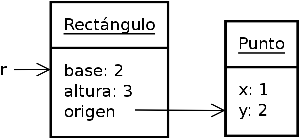
\includegraphics{graficos/15_Rectangulo_Punto}
\caption{Estado de las variables, al momento de crear el rectángulo}
\label{rectangulo_punto}
\end{figure}

El punto que describe la posición de la esquina inferior izquierda del
rectángulo es un objeto \lstinline!Punto!. El atributo \lstinline!origen!
contiene una {\it referencia} a dicho objeto.

Utilizando el método \lstinline!trasladar!, podemos modificar el valor del
punto contenido dentro del rectángulo.

\begin{codigo-python-sn}
>>> r.trasladar(2, 4)
>>> str(r)
Origen: (3, 6), Base: 2, Altura: 3
\end{codigo-python-sn}

También es posible directamente reemplazar el punto contenido, por un nuevo
punto.

\begin{codigo-python-sn}
>>> q = Punto(7, 2)
>>> r.origen = q
>>> str(r)
Origen: (7, 2), Base: 2, Altura: 3
\end{codigo-python-sn}

Con lo cual el diagrama pasa a ser el de la Figura
\ref{rectangulo_punto_b}.

\begin{figure}[htb]
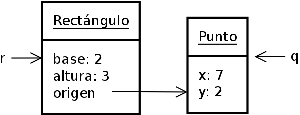
\includegraphics{graficos/15_Rectangulo_Punto_b}
\caption{Estado de las variables, luego de reemplazar el origen}
\label{rectangulo_punto_b}
\end{figure}

\begin{observacion}
El \lstinline!Punto(1, 2)! y \lstinline!Punto(3,6)! que habían sido creados
previamente, están ahora fuera de uso, por lo que quedan a disposición de un
mecanismo de {\it recolección de basura} que se encarga de recuperar
automáticamente las secciones de memoria que quedan fuera de uso durante la
ejecución de un programa.
\end{observacion}

\section{Resumen}

\begin{itemize}
\item Se llama {\bf polimorfismo} a la posibilidad de obtener distintos
comportamientos mediante la invocación a métodos de un mismo nombre, pero de
clases distintas.

\item Se llama {\bf herencia} a la relación entre clases en la cual una es una
clase base y otra es una clase derivada, que {\it hereda} los métodos y
atributos de la clase base.

\item Se llama {\bf delegación} a la relación entre clases en la cual una
instancia de una clase contiene como atributo una instancia de otra clase,
y dentro de sus métodos realiza invocaciones a los métodos de la clase
contenida.

\item Se denomina {\bf referencia} a las variables que permiten acceder a
un determinado objeto, ya sea un atributo dentro de un objeto, o una
variable en una porción de código cualquiera.
\end{itemize}


\newpage
\section{Ejercicios}

\extractionlabel{guia}
\begin{ejercicio}
{\bf Papel, Birome, Marcador}
\begin{partes}
    \item Escribir una clase {\it Papel} que contenga un texto, un método {\it
escribir}, que reciba una cadena para agregar al texto, y el método {\it
\_\_str\_\_} que imprima el contenido del texto.
    \item Escribir una clase {\it Birome} que contenga una cantidad de tinta, y
un método {\it escribir}, que reciba un texto y un papel sobre el cual
escribir. Cada letra escrita debe reducir la cantidad de tinta contenida.
Cuando la tinta se acabe, debe lanzar una excepción.
    \item Escribir una clase {\it Marcador} que herede de Birome, y agregue el
método {\it recargar}, que reciba la cantidad de tinta a agregar.
\end{partes}
\end{ejercicio}


\extractionlabel{guia}
\begin{ejercicio}
{\bf Juego de Rol}
\begin{partes}
    \item Escribir una clase {\it Personaje} que contenga los atributos {\it
vida}, {\it posicion} y {\it velocidad}, y los métodos {\it
recibir\_ataque}, que reduzca la vida según una cantidad recibida y lance
una excepción si la vida pasa a ser menor o igual que cero, y {\it
mover} que reciba una dirección y se mueva en esa dirección la cantidad
indicada por velocidad.
    \item Escribir una clase {\it Soldado} que herede de Personaje, y agregue
el atributo {\it ataque} y el método {\it atacar}, que reciba otro
personaje, al que le debe hacer el daño indicado por el atributo ataque.
    \item Escribir una clase {\it Campesino} que herede de Personaje, y agregue
el atributo {\it cosecha} y el método {\it cosechar}, que devuelva la
cantidad cosechada.
\end{partes}
\end{ejercicio}


\chapter{Listas enlazadas}

En esta unidad nos dedicaremos a construir nuestras propias listas, que
consistirán de cadenas de objetos enlazadas mediante referencias, como las
vistas en la unidad anterior.

Si bien Python ya cuenta con sus propias listas, las listas enlazadas que
implementaremos en esta unidad nos resultarán también útiles.

\section{Una clase sencilla de {\it vagones}}

En primer lugar, definiremos una clase muy simple, \lstinline!Nodo!, que se
comportará como un vagón: tendrá sólo dos atributos: \lstinline!dato!, que
servirá para almacenar cualquier información, y \lstinline!prox!, que servirá
para poner una referencia al siguiente vagón.

Además, como siempre, implementaremos el constructor y el método
\lstinline!__str__! para poder obtener una representación en cadena de texto.

\begin{codigo-python-sn}
class Nodo:
    def __init__(self, dato=None, prox=None):
        self.dato = dato
        self.prox = prox

    def __str__(self):
        return str(self.dato)
\end{codigo-python-sn}

\begin{sabias_que}
Al implementar una función o un método, Python nos permite definir valores por
omisión para sus parámetros, con la notación |parametro=valor|. Por ejemplo, si
definimos la función:

\begin{codigo-python-sn}
def saludar(nombre="?"):
    return "¡Hola, {}!".format(nombre)
\end{codigo-python-sn}

\noindent al invocarla podemos omitir el parámetro |nombre|, en cuyo caso se le
asignará el valor |"?"|:

\begin{codigo-python-sn}
>>> saludar("Alan")
'¡Hola, Alan!'
>>> saludar()
'¡Hola, ?!'
\end{codigo-python-sn}
\end{sabias_que}

Ejecutamos este código:

\begin{codigo-python-sn}
>>> n3 = Nodo("Bananas")
>>> n2 = Nodo("Peras", n3)
>>> n1 = Nodo("Manzanas", n2)
>>> str(n1)
'Manzanas'
>>> str(n2)
'Peras'
>>> str(n3)
'Bananas'
\end{codigo-python-sn}

Con esto hemos generado la estructura de la Figura \ref{nodos}.

\begin{figure}[htb]
\begin{tikzpicture}
\node[umlattr,anchor=west]                                  (dato) {dato: "Manzanas"};
\node[umlattr,below=of dato.south west,anchor=north west]   (prox1) {prox:};
\node[umlattrs,fit=(prox1) (dato)] (attrs)  {};
\node[umltitle,above=of attrs]               (titulo) {Nodo};
\node[umlclass,fit=(titulo) (attrs)]         (n1)   {};
\draw[-] (titulo.south-|n1.west)--(titulo.south-|n1.east);

\node[umlattr,above=0.5cm of n1] (v1) {v1};
\draw[flecha] (v1.south)--(n1.north);

\node[umlattr,anchor=west,right=1cm of dato.east]           (dato) {dato: "Peras"};
\node[umlattr,below=of dato.south west,anchor=north west]   (prox2) {prox:};
\node[umlattrs,fit=(prox2) (dato)] (attrs)  {};
\node[umltitle,above=of attrs]               (titulo) {Nodo};
\node[umlclass,fit=(titulo) (attrs)]         (n2)   {};
\draw[-] (titulo.south-|n2.west)--(titulo.south-|n2.east);

\node[umlattr,above=0.5cm of n2] (v2) {v2};
\draw[flecha] (v2.south)--(n2.north);
\draw[flecha] (prox1.east)--(prox1-|n2.west);

\node[umlattr,anchor=west,right=1cm of dato.east]           (dato) {dato: "Bananas"};
\node[umlattr,below=of dato.south west,anchor=north west]   (prox3) {prox:};
\node[umlattrs,fit=(prox3) (dato)] (attrs)  {};
\node[umltitle,above=of attrs]               (titulo) {Nodo};
\node[umlclass,fit=(titulo) (attrs)]         (n3)   {};
\draw[-] (titulo.south-|n3.west)--(titulo.south-|n3.east);

\node[umlattr,above=0.5cm of n3] (v3) {v3};
\draw[flecha] (v3.south)--(n3.north);
\draw[flecha] (prox2.east)--(prox2-|n3.west);

\node[draw,inner sep=0pt,minimum height=0pt,minimum width=0.5cm,line width=1.5pt,right=0.5cm of n3.south east] (none) {};

\path[flecha] (prox3.east) -| (none);
\end{tikzpicture}
\caption{Nodos enlazados}
\label{nodos}
\end{figure}

El atributo \lstinline!prox! de \lstinline!n3! tiene una referencia nula,
lo que indica que \lstinline!n3! es el último vagón de nuestra estructura.

Hemos creado una lista en forma manual. Si nos interesa recorrerla, podemos
hacer lo siguiente:

\begin{codigo-python-sn}
def ver_lista(nodo):
    """Recorre todos los nodos a través de sus enlaces,
       mostrando sus contenidos."""

    while nodo is not None:
        print(nodo)
        nodo = nodo.prox
\end{codigo-python-sn}

\begin{codigo-python-sn}
>>> ver_lista(n1)
Manzanas
Peras
Bananas
\end{codigo-python-sn}

Es interesante notar que la estructura del recorrido de la lista es el
siguiente:

\begin{itemize}
\item Se le pasa a la función sólo la referencia al primer nodo.

\item El resto del recorrido se consigue siguiendo la cadena de
referencias dentro de los nodos.
\end{itemize}

Si se desea {\it desenganchar} un vagón del medio de la lista, alcanza con
cambiar la referencia |prox|:

\begin{codigo-python-sn}
>>> n1.prox = n3
>>> ver_lista(n1)
Manzanas
Bananas
>>> n1.prox = None
>>> ver_lista(n1)
Manzanas
\end{codigo-python-sn}

De esta manera también se pueden generar estructuras impensables:
¿qué sucede si escribimos \lstinline!n1.prox = n1!? La representación es finita
y sin embargo en este caso \lstinline!ver_lista(n1)! no termina nunca. Hemos
creado una {\it lista infinita}, también llamada {\it lista circular}.

% Este ejercicio no se entiende
%\ejercicioc{¿Cuál es la mejor manera
%de tener siempre manzanas y peras a disposición de uno?}

\subsection{Caminos}

En una lista implementada con nodos, si seguimos las flechas
dadas por las referencias, obtenemos un {\it camino} en la lista.

Los caminos cerrados se denominan {\it ciclos}. Son ciclos, por ejemplo, la
autorreferencia de \lstinline|n1| a \lstinline|n1|, como así también una
flecha de \lstinline|n1| a \lstinline|n2| seguida de una flecha de
\lstinline|n2| a \lstinline|n1|.

\begin{atencion}
Las listas circulares no tienen nada de malo en sí mismas,
mientras su representación sea finita. El problema, en cambio, es que debemos tener
mucho cuidado al escribir programas para recorrerlas, ya que el recorrido
debe ser acotado (por ejemplo no habría problema en ejecutar un programa
que liste los 20 primeros nodos de una lista circular).

Cuando una función recibe una lista y el recorrido no está acotado,
se debe aclarar en su precondición que la ejecución de la misma terminará
sólo si la lista no contiene ciclos. Ése es el caso de la función
\lstinline|ver_lista(n1)|.
\end{atencion}

\subsection{Referenciando el principio de la lista}

Una cuestión no contemplada hasta el momento es la de mantener una referencia
a la lista completa. Por ahora para nosotros la lista es la colección de nodos
que se enlazan a partir de \lstinline|n1|. Sin embargo puede suceder que queramos
quitar a \lstinline|n1| y continuar con el resto de la lista como la colección de
nodos a tratar.

Una solución muy simple es asociar una referencia al principio de la lista,
que llamaremos \lstinline|lista|, y que mantendremos independientemente de cuál sea
el nodo que está al principio de la lista:

\begin{codigo-python-sn}
>>> n3 = Nodo("Bananas")
>>> n2 = Nodo("Peras", n3)
>>> n1 = Nodo("Manzanas", n2)
>>> lista = n1
>>> ver_lista(lista)
Manzanas
Peras
Bananas
\end{codigo-python-sn}

Ahora sí estamos en condiciones de eliminar el primer elemento de la lista
sin perder la identidad de la misma:

\begin{codigo-python-sn}
>>> lista = lista.prox
>>> ver_lista(lista)
Peras
Bananas
\end{codigo-python-sn}

\section{Tipos abstractos de datos}

Los tipos nuevos que habíamos definido en unidades anteriores fueron tipos de
datos concretos: un punto se definía como un par ordenado de números, un hotel
se definía por dos cadenas de caracteres (nombre y unicación) y dos números
(calidad y precio), etc.

Vamos a ver ahora una nueva manera de definir datos: por las
operaciones que tienen y por lo que tienen que hacer esas
operaciones (cuál es el resultado esperado de esas operaciones).

Esa manera de definir datos se conoce como {\it tipos abstractos de datos} o
{\it TADs}.

Lo novedoso de este enfoque respecto del anterior es que en general se puede
encontrar más de una representación mediante tipos concretos para representar
el mismo TAD, y que se puede elegir la representación más conveniente en cada
caso, según el contexto de uso.

Los programas que los usan hacen referencia a las operaciones que tienen, no a
la representación, y por lo tanto ese programa sigue funcionando si se cambia
la representación.

Dentro del ciclo de vida de un TAD hay dos fases: la programación del TAD y
la construcción de los programas que lo usan.

Durante la fase de programación del TAD, habrá que elegir una
representación, y luego programar cada uno de los métodos sobre esa
representación.

Durante la fase de construcción de los programas, no será relevante para el
programador que utiliza el TAD cómo está implementado, sino únicamente los
métodos que posee.

\begin{observacion}
Utilizando el concepto de \emph{interfaz} visto en la unidad anterior, podemos
decir que a quien utilice el TAD sólo le interesará la interfaz que éste
ofrezca.
\end{observacion}

\section{La clase {\tt ListaEnlazada}}

Basándonos en los nodos implementados anteriormente, pero buscando
desligar al programador que desea usar la lista de la responsabilidad de
manipular las referencias, definiremos ahora la clase
\lstinline!ListaEnlazada!, de modo tal que no haya que operar mediante las
referencias internas de los nodos, sino que se lo pueda hacer a través de
operaciones de lista.

Más allá de la implementación en particular, se podrá notar que implementaremos
los mismos métodos de las listas de Python, de modo que más allá del
funcionamiento interno, ambas serán {\bf listas}.

Definimos a continuación las operaciones que inicialmente deberá cumplir la
clase \lstinline!ListaEnlazada!.

\begin{itemize}
\item \lstinline|__str__|, para obtener una representación en cadena de texto.

\item \lstinline|__len__|, para calcular la longitud de la lista.

\item \lstinline|append(x)|, para agregar un elemento al final de la lista.

\item \lstinline|insert(i, x)|, para agregar el elemento \lstinline!x! en la
posición \lstinline!i! (levanta una excepción si la posición \lstinline!i! es
inválida).

\item \lstinline|remove(x)|, para eliminar la primera aparición de
\lstinline!x! en la lista (levanta una excepción si \lstinline!x! no está).

\item \lstinline|pop([i])|, para eliminar el elemento que está en la posición
\lstinline!i! y devolver su valor. Si no se especifica el valor de
\lstinline!i!, \lstinline|pop()| elimina y devuelve el elemento que está en
el último lugar de la lista (levanta una excepción si se hace referencia a
una posición no válida de la lista).

\item \lstinline|index(x)|, devuelve la posición de la primera aparición de
\lstinline!x! en la lista (levanta una excepción si \lstinline!x! no está).
\end{itemize}

Más adelante podrá agregarse a la lista otros métodos que también están
implementados por las listas de Python.

Valen ahora algunas consideraciones más antes de empezar a implementar la clase:

\begin{itemize}

\item Por lo dicho anteriormente, es claro que la lista deberá tener como
atributo la referencia al primer nodo que la compone.

\item Una implementación trivial del método |__len__| podría
recorrer todos los nodos de la lista y contar la cantidad de elementos,
pero si la lista tiene muchos elementos esto podría ser poco eficiente.

Para mejorar la eficiencia alcanza con agregar un atributo numérico que
contenga la cantidad de nodos. Así, este atributo que llamaremos |len|
se inicializará en $0$ cuando se cree la lista vacía, se
incrementará en $1$ cada vez que se agregue un elemento y se decrementará en $1$
cada vez que se elimine un elemento.

\begin{atencion}
Al agregar el atributo |len| estamos {\it duplicando información}, ya que habrá
dos formas de obtener la longitud de la lista:

\begin{enumerate}
\item contar los nodos
\item obtener el valor de |len|
\end{enumerate}

Como consecuencia, vamos a tener que prestar especial atención para que el
atributo |len| siempre contenga un valor consistente; es decir que su valor sea
siempre igual a la cantidad de nodos que contiene la lista.

En la sección \ref{invariante-objetos} se explica más formalmente este
concepto.
\end{atencion}

\item Por otro lado, como vamos a incluir todas las operaciones de listas
que sean necesarias para operar con ellas, no es necesario que la clase
\lstinline!Nodo! esté disponible para que otros programadores puedan
modificar (y romper) las listas a voluntad usando operaciones de nodos. Para eso
incluiremos la clase \lstinline!Nodo! de manera {\it privada} (es
decir oculta), de modo que la podamos usar nosotros como dueños
(fabricantes) de la clase, pero no cualquier programador que utilice la
lista.
\end{itemize}

Python tiene una convención para hacer que atributos, métodos o clases
dentro de una clase dada no puedan ser usados por los usuarios, y sólo
tengan acceso a ellos quienes programan la clase: su nombre tiene que
empezar con un guión bajo y terminar sin guión bajo. Así que para hacer que
los nodos sean privados, cambiaremos el nombre de la clase a \lstinline|_Nodo|.

\begin{observacion}
Se trata sólo de una convención, aun con el nombre \lstinline!_Nodo! la
clase está disponible, pero respetaremos esa convención de aquí en adelnte.
\end{observacion}

\subsection{Construcción de la lista}

Empezamos escribiendo la clase con su constructor.

\begin{codigo-python-sn}
class ListaEnlazada:
    """Modela una lista enlazada."""

    def __init__(self):
        """Crea una lista enlazada vacía."""
        # referencia al primer nodo (None si la lista está vacía)
        self.prim = None
        # cantidad de elementos de la lista
        self.len = 0
\end{codigo-python-sn}

Nuestra estructura ahora será como la representada por la Figura
\ref{lista_enlazada}.

\begin{figure}[htb]
\begin{tikzpicture}
\node[umlattr,anchor=west]                                  (len) {len: 2};
\node[umlattr,below=of len.south west,anchor=north west]   (prim) {prim:};
\node[umlattrs,fit=(prim) (len)] (attrs)  {};
\node[umltitle,above=of attrs]               (titulo) {ListaEnlazada};
\node[umlclass,fit=(titulo) (attrs)]         (n1)   {};
\draw[-] (titulo.south-|n1.west)--(titulo.south-|n1.east);

\node[umlattr,anchor=west,right=2cm of len.east]           (dato) {dato: "Peras"};
\node[umlattr,below=of dato.south west,anchor=north west]   (prox2) {prox:};
\node[umlattrs,fit=(prox2) (dato)] (attrs)  {};
\node[umltitle,above=of attrs]               (titulo) {Nodo};
\node[umlclass,fit=(titulo) (attrs)]         (n2)   {};
\draw[-] (titulo.south-|n2.west)--(titulo.south-|n2.east);

\draw[flecha] (prim.east)--(prim-|n2.west);

\node[umlattr,anchor=west,right=1cm of dato.east]           (dato) {dato: "Bananas"};
\node[umlattr,below=of dato.south west,anchor=north west]   (prox3) {prox:};
\node[umlattrs,fit=(prox3) (dato)] (attrs)  {};
\node[umltitle,above=of attrs]               (titulo) {Nodo};
\node[umlclass,fit=(titulo) (attrs)]         (n3)   {};
\draw[-] (titulo.south-|n3.west)--(titulo.south-|n3.east);

\draw[flecha] (prox2.east)--(prox2-|n3.west);
\node[draw,inner sep=0pt,minimum height=0pt,minimum width=0.5cm,line width=1.5pt,right=0.5cm of n3.south east] (none) {};

\path[flecha] (prox3.east) -| (none);
\end{tikzpicture}
\caption{Una lista enlazada}
\label{lista_enlazada}
\end{figure}

\ejercicioc{Escribir los métodos \lstinline!__str__! y \lstinline!__len__!
para la lista}.

\begin{sabias_que}
Una característica importante de la implementación de listas enlazadas es que
eliminar el primer elemento es una operación de {\it tiempo constante}, es
decir que no depende de la longitud de la lista. En las listas de
Python, por contraste, esta operación requiere un {\it tiempo proporcional a la
longitud de la lista}.

Sin embargo no todo es tan positivo: el acceso a la posición $p$ se realiza
en {\it tiempo proporcional a $p$}, mientras que en las listas de Python esta
operación se realiza en {\it tiempo constante}.

Conociendo las ventajas y desventajas podremos elegir el tipo de lista que
necesitemos según los requerimientos de cada problema.
\end{sabias_que}

\subsection{Eliminar un elemento de una posición}

Analizaremos a continuación \lstinline|pop([i])|, que elimina el elemento que
está en la posición \lstinline!i! y devuelve su valor. Si no se especifica
el valor de \lstinline!i!, \lstinline|pop()| elimina y devuelve el elemento
que está en el último lugar de la lista.  Por otro lado, levanta una
excepción si se hace referencia a una posición no válida de la lista.

Dado que se trata de una función con cierta complejidad, separaremos el
código en las diversas consideraciones a tener en cuenta.

\begin{itemize}

\item Si la posición es inválida (\lstinline!i! menor que $0$ o mayor o
igual a la longitud de la lista), se considera error y se levanta la
excepción |IndexError|.

Esto se resuelve con este fragmento de código:

\begin{codigo-python-sn}
if i < 0 or i >= self.len:
    raise IndexError("Índice fuera de rango")
\end{codigo-python-sn}

\item Si no se indica posición, \lstinline!i! toma la última posición de la
lista:

\begin{codigo-python-sn}
if i is None:
    i = self.len - 1
\end{codigo-python-sn}

\item Cuando la posición es $0$ se trata de un caso particular, ya que en ese
caso hay que cambiar la referencia de
\lstinline!self.prim! para que apunte al nodo siguiente.  Es decir, pasar de
\lstinline!self.prim! $\rightarrow$ |nodo0| $\rightarrow$ |nodo1| a
\lstinline!self.prim! $\rightarrow$ |nodo1|).

\begin{codigo-python-sn}
if i == 0:
    dato = self.prim.dato
    self.prim = self.prim.prox
\end{codigo-python-sn}

\noindent (Guardamos el |dato| del nodo descartado para poder devolverlo al
finalizar la función).

\item Vemos ahora el caso general:

Mediante un ciclo, se deben ubicar los nodos $n_{i - 1}$ y $n_i$ que
están en las posiciones $i-1$ e $i$ de la lista, respectivamente, de modo de
poder ubicar no sólo el nodo que se descartará, sino también estar en condiciones
de saltear el nodo descartado en los enlaces de la lista.  La lista debe pasar de
contener el camino $n_{i-1} \rightarrow n_i \rightarrow n_{i+1}$
a contener el camino $n_{i-1} \rightarrow n_{i+1}$.

Nos basaremos un esquema muy simple y útil que se denomina {\it máquina de parejas}:

Si nuestra secuencia tiene la forma $ABCDE$, se itera sobre ella de modo de
tener las parejas $AB$, $BC$, $CD$, $DE$. En la pareja $XY$, llamaremos a $X$ el
{\it elemento anterior}
y a $Y$ el {\it elemento actual}. En general estos ciclos terminan o bien cuando
no hay más parejas que formar, o bien cuando el elemento actual cumple con una determinada
condición.

En nuestro problema, tenemos la siguiente situación:

\begin{itemize}
\item Las parejas son parejas de nodos.

\item Para avanzar en la secuencia se usa la referencia al próximo nodo de la lista.

\item La condición de terminación es siempre que la posición del nodo en la
lista sea igual al valor buscado.  En este caso particular no debemos
preocuparnos por la terminación de la lista porque la validez del índice
buscado ya fue verificada más arriba.
\end{itemize}

Esta es la porción de código correspondiente a la búsqueda. Llamamos |n_ant| y
|n_act| a los elementos anterior y actual de la pareja de nodos:

\begin{codigo-python-sn}
n_ant = self.prim
n_act = n_ant.prox
for pos in range(1, i):
    n_ant = n_act
    n_act = n_ant.prox
\end{codigo-python-sn}

Al finalizar el ciclo, \lstinline!n_ant! será una referencia al nodo $i-1$ y
\lstinline!n_act! una referencia al nodo $i$.

Una vez obtenidas las referencias, se obtiene el dato y se cambia el camino
para descartar el nodo |n_act|:

\begin{codigo-python-sn}
dato = n_act.dato
n_ant.prox = n_act.prox
\end{codigo-python-sn}

\item Finalmente, en todos los casos de éxito se debe devolver el dato que contenía
el nodo descartado y decrementar la longitud en 1:

\begin{codigo-python-sn}
self.len -= 1
return dato
\end{codigo-python-sn}

\end{itemize}

Finalmente, en el Código \ref{lista_enlazada_pop} se incluye el código completo
del método \lstinline!pop!.

\begin{codigo}{pop}{Método pop de la lista enlazada}
\label{lista_enlazada_pop}
\begin{codigo-python}
def pop(self, i=None):
    """Elimina el nodo de la posición i, y devuelve el dato contenido.
       Si i está fuera de rango, se levanta la excepción IndexError.
       Si no se recibe la posición, devuelve el último elemento."""

    if i is None:
        i = self.len - 1

    if i < 0 or i >= self.len:
        raise IndexError("Índice fuera de rango")

    if i == 0:
        # Caso particular: saltear la cabecera de la lista
        dato = self.prim.dato
        self.prim = self.prim.prox
    else:
        # Buscar los nodos en las posiciones (i-1) e (i)
        n_ant = self.prim
        n_act = n_ant.prox
        for pos in range(1, i):
            n_ant = n_act
            n_act = n_ant.prox

        # Guardar el dato y descartar el nodo
        dato = n_act.dato
        n_ant.prox = n_act.prox

    self.len -= 1
    return dato
\end{codigo-python}
\end{codigo}

\subsection{Eliminar un elemento por su valor}

Análogamente se resuelve \lstinline|remove(self, x)|, que debe eliminar la
primera aparición de \lstinline!x! en la lista, o bien levantar una excepción
si \lstinline!x! no se encuentra en la lista.

Nuevamente, dado que se trata de un método de cierta complejidad, lo
resolveremos por partes, teniendo en cuenta los casos particulares y el caso
general.

\begin{itemize}

\item Si la lista está vacía levantamos una excepción. Tenemos que tratarlo
como un caso particular, ya que en todos los siguientes casos necesitamos
que haya al menos un nodo.

\begin{codigo-python-sn}
if self.prim is None
    raise ValueError("La lista está vacía")
\end{codigo-python-sn}

\item El caso en el que x está en el primer nodo también es particular, ya
que modificar la referencia |self.prim|:

\begin{codigo-python-sn}
if self.prim.dato == x:
    self.prim = self.prim.prox
\end{codigo-python-sn}

\item El caso general también implica un recorrido con máquina de parejas, sólo
que esta vez la condición de terminación es: o bien la lista se terminó o bien
encontramos un nodo con el valor \lstinline!x! buscado.

\begin{codigo-python-sn}
n_ant = self.prim
n_act = n_ant.prox
while n_act is not None and n_act.dato != x:
    n_ant = n_act
    n_act = n_ant.prox
\end{codigo-python-sn}

En este caso, al terminarse el ciclo será necesario corroborar si se terminó
porque llegó al final de la lista, y de ser así levantar una excepción; o si se
terminó porque encontró el dato, y de ser así eliminarlo.

\begin{codigo-python-sn}
if n_act is None:
    raise ValueError("El valor no está en la lista.")
n_ant.prox = n_act.prox
\end{codigo-python-sn}

\item Finalmente, en todos los casos de éxito debemos decrementar en 1 el valor
de \lstinline|self.len|.

\end{itemize}

En el Código \ref{lista_enlazada_remove} se incluye el código completo
del método \lstinline!remove!.

\begin{codigo}{remove}{Método remove de la lista enlazada}
\label{lista_enlazada_remove}
\begin{codigo-python}
def remove(self, x):
    """Borra la primera aparición del valor x en la lista.
       Si x no está en la lista, levanta ValueError"""

    if self.len == 0:
        raise ValueError("Lista vacía")

    if self.prim.dato == x:
        # Caso particular: saltear la cabecera de la lista
        self.prim = self.prim.prox
    else:
        # Buscar el nodo anterior al que contiene a x (n_ant)
        n_ant = self.prim
        n_act = n_ant.prox
        while n_act is not None and n_act.dato != x:
            n_ant = n_act
            n_act = n_ant.prox

        if n_act == None:
            raise ValueError("El valor no está en la lista.")

        # Descartar el nodo
        n_ant.prox = n_act.prox

    self.len -= 1
\end{codigo-python}
\end{codigo}

\subsection{Insertar nodos}

Debemos programar ahora \lstinline|insert(i, x)|, que debe agregar el elemento
\lstinline!x! en la posición \lstinline!i!  (y levantar una excepción si la
posición \lstinline!i! es inválida).

Veamos qué debemos tener en cuenta para programar esta función.

\begin{itemize}

\item Si se intenta insertar en una posición menor que cero o mayor que la
longitud de la lista debe levantarse una excepción.

\begin{codigo-python-sn}
if i < 0 or i > self.len:
    raise IndexError("Posición inválida")
\end{codigo-python-sn}

\item Para los demás casos hay que crear un nodo, que será el que se insertará
en la posición que corresponda. Construimos un nodo \lstinline|nuevo| cuyo
\lstinline|dato| será \lstinline|x|.

\begin{codigo-python-sn}
nuevo = _Nodo(x)
\end{codigo-python-sn}

\item Si se quiere insertar en la posición 0, hay que cambiar la referencia de
\lstinline|self.prim|.

\begin{codigo-python-sn}
if i == 0:
    nuevo.prox = self.prim
    self.prim = nuevo
\end{codigo-python-sn}

\item Para los demás casos, nuevamente será necesaria la máquina de parejas.
Obtenemos el nodo anterior a la posición en la que queremos insertar.

\begin{codigo-python-sn}
n_ant = self.prim
for pos in range(1, i):
    n_ant = n_ant.prox

nuevo.prox = n_ant.prox
n_ant.prox = nuevo
\end{codigo-python-sn}

\item En todos los casos de éxito se debe incrementar en 1 la longitud de la lista.

\end{itemize}

En el Código \ref{lista_enlazada_insert} se incluye el código resultante
del método \lstinline!insert!.

\begin{codigo}{insert}{Método insert de la lista enlazada}
\label{lista_enlazada_insert}
\begin{codigo-python}
def insert(self, i, x):
    """Inserta el elemento x en la posición i.
       Si la posición es inválida, levanta IndexError"""

    if i < 0 or i > self.len:
        raise IndexError("Posición inválida")

    nuevo = _Nodo(x)

    if i == 0:
        # Caso particular: insertar al principio
        nuevo.prox = self.prim
        self.prim = nuevo
    else:
        # Buscar el nodo anterior a la posición deseada
        n_ant = self.prim
        for pos in range(1, i):
            n_ant = n_ant.prox

        # Intercalar el nuevo nodo
        nuevo.prox = n_ant.prox
        n_ant.prox = nuevo

    self.len += 1
\end{codigo-python}
\end{codigo}

\ejercicioc{Completar la clase \lstinline|ListaEnlazada| con los métodos que
faltan: \lstinline|append| e \lstinline|index|}.

\ejercicioc{En los bucles de {\it máquina de parejas} mostrados
anteriormente, no siempre es necesario tener la referencia al nodo actual,
puede alcanzar con la referencia al nodo anterior.  Donde sea posible,
eliminar la referencia al nodo actual.  Una vez hecho esto, analizar el
código resultante, ¿Es más elegante?}

\ejercicioc{\label{append_constante} {\bf Mantenimiento:} Con esta representación conseguimos que la
inserción en la posición 0 se realice en tiempo constante, sin embargo ahora
\lstinline|append| es lineal en la longitud de la lista. Si queremos mejorar
esto, debemos agregar un atributo más a los objetos de la
clase: la referencia al último nodo, y modificar \lstinline|append| para que se
pueda ejecutar en tiempo constante. Por supuesto que además hay que modificar
todos los métodos de la clase para que se mantenga la propiedad de que ese
atributo siempre es una referencia al útimo nodo.}

\section{Invariantes de objetos}

\label{invariante-objetos}
Los invariantes son condiciones que deben ser siempre ciertas.  En la sección
\ref{invariantes} mencionamos los invariantes de ciclos, que son condiciones que deben
permanecer ciertas durante la ejecución de un ciclo.  Existen también los
invariantes de objetos, que son condiciones que deben ser ciertas a lo
largo de toda la existencia de un objeto.

La clase \lstinline!ListaEnlazada! presentada en la sección anterior,
cuenta con dos invariantes que siempre debemos mantener.  Por un lado, el
atributo \lstinline!len! debe contener siempre la cantidad de nodos de la
lista.  Es decir, siempre que se modifique la lista, agregando o quitando
un nodo, se debe actualizar \lstinline!len! como corresponda.

Por otro lado, el atributo \lstinline!prim! referencia siempre al primer
nodo de la lista. Si se agrega o elimina este primer nodo, es necesario
actualizar esta referencia.

Cuando se desarrolla una estructura de datos como la lista enlazada, es
importante destacar cuáles serán sus invariantes, ya que en cada método
habrá que tener especial cuidado de que los invariantes permanezcan siempre
ciertos.

Así, si se modifica la lista para que la inserción al final pueda hacerse en
tiempo constante (como se pide en el ejercicio \ref{append_constante}),
se está agregando a la lista un nuevo invariante (un atributo de la lista
que apunte siempre al último elemento) y no es sólo el método
\lstinline!append! el que hay que modificar, sino todos los métodos que
puedan de una u otra forma cambiar la referencia al último elemento de la
lista.

\section{Otras listas enlazadas}

Las listas presentadas hasta aquí son las {\it listas simplemente
enlazadas}, que son sencillas y útiles cuando se quiere poder insertar o
eliminar nodos de una lista en tiempo constante.

Existen otros tipos de listas enlazadas, cada uno con sus ventajas y
desventajas.

\subsection*{Listas doblemente enlazadas}

Las listas doblemente enlazadas son aquellas en que los nodos cuentan no
sólo con una referencia al siguiente, sino también con una referencia al
anterior.  Esto permite que la lista pueda ser recorrida en ambas
direcciones.

En una lista doblemente enlazada es posible, por ejemplo, eliminar un
nodo sin necesidad de saber cuál es el anterior.

Entre las desventajas podemos mencionar que al tener que mantener dos
referencias el código se vuelve más complejo, y también que ocupa más
espacio en memoria.

\subsection*{Listas circulares}

Las listas circulares, que ya fueron mencionadas al comienzo de esta
unidad, son aquellas en las que el último nodo contiene una referencia al
primero.  Pueden ser tanto simplemente como doblemente enlazadas.

Se las utiliza para modelar situaciones en las cuales los elementos no
tienen un primero o un último, sino que forman una cadena infinita, que se
recorre una y otra vez.

\begin{sabias_que}
El código del kernel Linux, que está programado en C, incluye una
implementación de lista enlazada circular utilizada en la mayoría de los
subsistemas.

Por ejemplo, la lista de tareas que se están ejecutando es una lista
circular.  El {\it scheduler} (planificador) del kernel permite que cada tarea
utilice el procesador durante una porción de tiempo y luego pasa a la
siguiente, aplicando así una ``ronda de turnos'' sin que haya una primera o una
última tarea.
\end{sabias_que}

\section{Iteradores}

En la unidad anterior se hizo referencia a que todas las secuencias
pueden ser recorridas mediante una misma estructura
(\lstinline!for variable in secuencia!), ya que todas implementan el método
especial \lstinline!__iter__!.  Este método debe devolver un {\it iterador}
capaz de recorrer la secuencia como corresponda.

\begin{observacion}
Un iterador es un objeto que permite recorrer uno a uno los elementos
almacenados en una estructura de datos, y operar con ellos.
\end{observacion}

Un ejemplo de iteradores que estuvimos usando desde la primera unidad es la
función |range|:

\begin{codigo-python-sn}
>>> r = range(3)
>>> type(r)
<class 'range'>
\end{codigo-python-sn}

Lo primero que observamos es que la función |range| no devuelve una lista de
números, sino que devuelve una instancia de la clase |range|. Para obtener un
iterador a partir de este objeto podemos aplicar la función |iter| (que a su
vez llamará al método |__iter__|):

\begin{codigo-python-sn}
>>> i = iter(r)
>>> type(i)
<class 'range_iterator'>
\end{codigo-python-sn}

En Python los iteradores implementan un método
\lstinline!__next__! que debe devolver los elementos, de a uno por vez,
comenzando por el primero.  Y al llegar al final de la estructura, debe
levantar una excepción de tipo \lstinline!StopIteration!.

La función |next| permite invocar manualmente al método |__next__|:

\begin{codigo-python-sn}
>>> next(i)
0
>>> next(i)
1
>>> next(i)
2
>>> next(i)
Traceback (most recent call last):
  File "<stdin>", line 1, in <module>
StopIteration
\end{codigo-python-sn}

Cuando hacemos |for x in range(3)|, el bucle |for| automáticamente llama a las
funciones |iter| y |next|, asignando a |x| los valores que devuelve |next| en
cada iteración.

Es decir que las siguientes estructuras son equivalentes:

\begin{codigo-python-sn}
for elemento in secuencia:
	# hacer algo con elemento
\end{codigo-python-sn}

\begin{codigo-python-sn}
iterador = iter(secuencia)
while True:
    try:
        elemento = next(iterador)
    except StopIteration:
        break
    # hacer algo con elemento
\end{codigo-python-sn}

\subsection*{Iterador para la lista enlazada}

Si queremos implementar un iterador para la lista enlazada,
la mejor solución implica crear una nueva clase,
\lstinline!_IteradorListaEnlazada!, que implemente el método
\lstinline!__next__! de la forma apropiada.

\begin{atencion}
Utilizamos la notación de clase privada, utilizada también para la clase
\lstinline!_Nodo!, ya que si bien se devolverá el iterador cuando sea
necesario, un programador externo no debería construir el iterador sin
pasar a través de la lista enlazada.
\end{atencion}

Para inicializar la clase, lo único que se necesita es una referencia al
primer elemento de la lista.

\begin{codigo-python-sn}
class _IteradorListaEnlazada:
    def __init__(self, prim):
        self.actual = prim
\end{codigo-python-sn}

A partir de allí, el iterador irá avanzando a través de los elementos de la
lista mediante el método \lstinline!__next__!.  Para verificar que no se haya
llegado al final de la lista, se corroborará que la referencia
\lstinline!self.actual! sea distinta de \lstinline!None!.

\begin{codigo-python-sn}
if self.actual is None:
    raise StopIteration()
\end{codigo-python-sn}

Una vez que se pasó la verificación, la primera llamada a \lstinline!__next__!
debe devolver el primer elemento, pero también debe avanzar, para que la
siguiente llamada devuelva el siguiente elemento.  Por ello, se utiliza la
estructura {\it guardar, avanzar, devolver}.

\begin{codigo-python-sn}
dato = self.actual.dato
self.actual = self.actual.prox
return dato
\end{codigo-python-sn}

En el Código \ref{iterador_enlazada} se puede ver el código completo del
iterador.

\begin{codigo}{\_IteradorListaEnlazada}{Un iterador para la lista enlazada}
\label{iterador_enlazada}
\begin{codigo-python}
class _IteradorListaEnlazada:
    def __init__(self, prim):
        self.actual = prim

    def __next__(self):
        if self.actual is None:
            raise StopIteration()

        dato = self.actual.dato
        self.actual = self.actual.prox
        return dato
\end{codigo-python}
\end{codigo}

Finalmente, es necesario modificar la clase \lstinline!ListaEnlazada! para que
devuelva una instancia del iterador
cuando se llama al método \lstinline!__iter__!.

\begin{codigo-python-sn}
    def __iter__(self):
        """Devuelve un iterador de la lista."""
        return _IteradorListaEnlazada(self.prim)
\end{codigo-python-sn}

Con todo esto será posible recorrer nuestra lista con la estructura a la
que estamos acostumbrados.

\begin{codigo-python-sn}
>>> l = ListaEnlazada()
>>> l.append(7)
>>> l.append(3)
>>> l.append(5)
>>> for valor in l:
...     print(valor)
...
7
3
5
\end{codigo-python-sn}

No solo eso, sino que además podremos utilizar la lista enlazada en cualquier
operación que requiera una secuencia {\it iterable}:

\begin{codigo-python-sn}
>>> list(l) # convertir a una lista de Python
[7, 3, 5]
>>> sum(l) # sumar los elementos
15
>>> max(l) # obtener el máximo elemento
7
\end{codigo-python-sn}

\section{Resumen}

\begin{itemize}

\item Un {\bf tipo abstracto de datos} (TAD) es un tipo de datos que está
definido por las operaciones que contiene y cómo se comportan (su {\it
interfaz}), no por la forma en la que esas operaciones están implementadas.

\item Una {\bf lista enlazada} es una implementación del TAD {\it lista}.
Se trata de una lista compuesta por nodos, en la que
cada nodo contiene un dato y una referencia al nodo que le sigue.

\item En las listas enlazadas, es {\it barato} insertar o eliminar
elementos, ya que simplemente se deben alterar un par de referencias; pero
es {\it caro} acceder a un elemento en particular, ya que es necesario
pasar por todos los anteriores para llegar a él.

\item Tanto al insertar como al remover elementos de una lista enlazada, se
utiliza la técnica de {\it máquina de parejas}, mediante la cual se va
recorriendo la lista hasta encontrar el lugar apropiado donde operar con
las referencias.

\item Una {\bf lista doblemente enlazada} es aquella cuyos nodos además del
dato contienen una referencia al nodo anterior y otra al nodo siguiente, de
modo que se la puede recorrer en ambos sentidos.

\item Una {\bf lista circular} es aquella en la que el último nodo contiene
una referencia al primero, y puede ser recorrida infinitamente.

\item Un {\bf iterador} es un objeto que permite recorrer uno a uno los
elementos de una secuencia.

\end{itemize}

\begin{referencia_python}

\begin{sintaxis}{\lstinline{__iter__(self)}}
Método especial que debe devolver un iterador para el objeto. El iterador debe
ser un objeto que implementa el método |__next__|.
\end{sintaxis}

\begin{sintaxis}{\lstinline{__next__(self)}}
Devuelve el elemento actual de la iteración y avanza al siguiente.
Si se llegó al final de la iteración lanza |StopIteration|.
\end{sintaxis}

\begin{sintaxis}{\lstinline{iter(objeto)}}
Equivalente a invocar |objeto.__iter__()|.
\end{sintaxis}

\begin{sintaxis}{\lstinline{next(objeto, [valor])}}
Equivalente a invocar |objeto.__next__()|. Si se invoca con el parámetro
adicional |valor|, al llegar al final de la iteración se devuelve el |valor| en
lugar de lanzar |StopIteration|.
\end{sintaxis}
\end{referencia_python}

\newpage
\section{Ejercicios}

\extractionlabel{guia}
\begin{ejercicio}
Agregar a la clase {\it ListaEnlazada} un método \verb!next! que vaya
devolviendo uno a uno cada elemento de la lista, desde el primero hasta el
último.  Al llegar al final de la lista debe levantar una excepción de la
clase {\it StopIteration}.  Para el correcto funcionamiento de este método, ¿es
necesario agregar un atributo adicional a la clase?
\end{ejercicio}

\extractionlabel{guia}
\begin{ejercicio}
Utilizando el método \verb!next! del ejercicio anterior, redefinir el
método \verb!__str__! de {\it ListaEnlazada}, para que se genere una salida
legible de lo que contiene la lista, similar a las listas de python. \\
{\bf Nota}: este método debe devolver una cadena, no imprimirla por
pantalla.
\end{ejercicio}

\extractionlabel{guia}
\begin{ejercicio}
Agregar a {\it ListaEnlazada} un método \verb!extend! que reciba una {\it
ListaEnlazada} y agregue a la lista actual los elementos que se encuentran
en la lista recibida.
\end{ejercicio}

% No es un buen ejemplo que LE Ordenada herede de LE ya que se tiene que bloquear
% o redefinir el significado del método append.
%
%\ejercicioc{
%Escribir una clase {\it ListaEnlazadaOrdenada} que herede de {\it
%ListaEnlazada}, redefiniendo el método \verb!insert! para que inserte los
%elementos de forma ordenada, y el método \verb!append! para que no permita
%la inserción al final.
%}

\extractionlabel{guia}
\begin{ejercicio}
Una {\bf lista circular} es una lista cuyo último nodo está ligado al primero,
de modo que es posible recorrerla infinitamente.  \\
Escribir la clase {\it ListaCircular}, incluyendo los métodos \verb!insert!,
\verb!append!, \verb!remove! y \verb!pop!.
\end{ejercicio}

\extractionlabel{guia}
\begin{ejercicio}
Una {\bf lista doblemente enlazada} es una lista en la cual cada nodo tiene
una referencia al anterior además de al próximo de modo que es posible
recorrerla en ambas direcciones. \\
Escribir la clase {\it ListaDobleEnlazada}, incluyendo los métodos
\verb!insert!, \verb!append!, \verb!remove! y \verb!pop!.
\end{ejercicio}

\extractionlabel{guia}
\begin{ejercicio}
Escribir un método de la clase {\it ListaEnlazada} que invierta el orden
de la lista (es decir, el primer elemento queda como último y
viceversa, y se invierte la dirección de todos los enlaces). \\
{\bf Nota}: operar directamente sobre los elementos de la lista.
\end{ejercicio}


\chapter{Pilas y colas}

En esta unidad veremos dos ejemplos de tipos abstractos de datos, de los más
clásicos: \emph{pilas} y \emph{colas}.

\section{Pilas}

Una \emph{pila} es un TAD que tiene las siguientes operaciones:

\begin{itemize}
\item \lstinline+__init__+: Inicializa una pila nueva, vacía.

\item \lstinline!apilar!: Agrega un nuevo elemento a la pila.

\item \lstinline!desapilar!: Elimina el tope de la pila y lo devuelve.
El elemento que se devuelve es siempre el último que se agregó.

\item \lstinline!esta_vacia!: Devuelve \lstinline!True! o \lstinline!False!
según si la pila está vacía o no.

\end{itemize}

El comportamiento de una pila se puede describir mediante la frase
``Lo último que se apiló es lo primero que se usa'', que es exactamente lo que
uno hace con una pila (de platos por ejemplo): en una pila de platos uno sólo
puede ver la apariencia completa del plato de arriba, y sólo puede tomar el
plato de arriba (si se intenta tomar un plato del medio de la pila lo más
probable es que alguno de sus vecinos, o él mismo, se arruine).

Como ya se dijo, al crear un tipo abstracto de datos, es importante decidir
cuál será la representación a utilizar.  En el caso de la pila, si bien puede
haber más de una representación, por ahora veremos la más sencilla:
representaremos una pila mediante una lista de Python.

Sin embargo, para los que construyen programas que usan un TAD vale el
siguiente llamado de atención:

\begin{atencion}
Al usar esa pila dentro de un programa, deberemos ignorar que se está
trabajando sobre una lista: solamente podremos usar los métodos de la
\emph{interfaz pila}.
\end{atencion}

\subsection{Pilas representadas por listas}

Definiremos una clase \lstinline!Pila! con un atributo \lstinline!items!,
de tipo lista, que contendrá los elementos de la pila. El tope de la pila
se encontrará en la última posición de la lista, y cada vez que se apile un
nuevo elemento, se lo agregará al final.

El método \lstinline+__init__+ no recibirá parámetros adicionales, ya que
deberá crear una pila vacía (que representaremos por una lista vacía):

\begin{codigo-python-sn}
class Pila:
    """Representa una pila con operaciones de apilar, desapilar y
       verificar si está vacía."""

    def __init__(self):
        """Crea una pila vacía."""
        self.items = []
\end{codigo-python-sn}

El método |esta_vacia| simplemente se fija si la lista de Python está vacía:

\begin{codigo-python-sn}
    def esta_vacia(self):
        """Devuelve True si la lista está vacía, False si no."""
        return len(self.items) == 0
\end{codigo-python-sn}

El método \lstinline!apilar! agrega el nuevo elemento al
final de la lista:

\begin{codigo-python-sn}
    def apilar(self, x):
        """Apila el elemento x."""
        self.items.append(x)
\end{codigo-python-sn}

Para implementar \lstinline!desapilar! se usamos el método \lstinline!pop!
de lista que hace exactamente lo requerido: elimina el último elemento de
la lista y devuelve el valor del elemento eliminado. Si la lista está vacía
|desapilar| lanza una excepción.

\begin{codigo-python-sn}
    def desapilar(self):
        """Devuelve el elemento tope y lo elimina de la pila.
           Si la pila está vacía levanta una excepción."""
        if self.esta_vacia():
            raise IndexError("La pila está vacía")
        return self.items.pop()
\end{codigo-python-sn}

\begin{observacion}
Utilizamos los métodos \lstinline!append! y \lstinline!pop! de las listas de
Python, porque sabemos que estos métodos se ejecutan en tiempo constante.
Queremos que el tiempo de apilar o desapilar de la pila no dependa de la
cantidad de elementos contenidos.
\end{observacion}

Construimos algunas pilas y operamos con ellas:

\begin{codigo-python-sn}
>>> p = Pila()
>>> p.esta_vacia()
True
>>> p.apilar(1)
>>> p.esta_vacia()
False
>>> p.apilar(5)
>>> p.apilar("+")
>>> p.apilar(22)
>>> p.desapilar()
22
>>> q = Pila()
>>> q.desapilar()
(^Traceback (most recent call last):
  File "<stdin>", line 1, in <module>
  File "Pila.py", line 24, in desapilar
    raise IndexError:("La pila está vacía")
IndexError: La pila está vacía^)
\end{codigo-python-sn}

\subsection{Uso de pila: calculadora científica}

La famosa calculadora portátil HP-35 (de 1972) popularizó la notación
polaca inversa (o notación prefijo) para hacer cálculos sin necesidad de
usar paréntesis. Esa notación, inventada por el lógico polaco Jan
Lukasiewicz en 1920, se basa en el principio de que un operador siempre se
escribe a continuación de sus operandos. La operación $(5-3)+8$ se
escribirá como \lstinline|5 3 - 8 +|, que se interpretará como: ``restar 3
de 5, y al resultado sumarle 8''.

Es posible implementar esta notación de manera sencilla usando una pila de
la siguiente manera, a partir de una cadena de entrada de valores separados
por blancos:

\begin{itemize}
\item Mientras se lean números, se apilan.

\item En el momento en el que se detecta una operación binaria |+|,
|-|, |*| o |/| se desapilan los dos últimos
números apilados, se ejecuta la operación indicada, y el resultado de esa
operación se apila.

\item Si la expresión está bien formada, tiene que quedar al final un único
número en la pila (el resultado).

\item Los posibles errores son:

\begin{itemize}
\item Queda más de un número al final (por ejemplo si la cadena de entrada
fue |"5 3"|),

\item Ingresa algún caracter que no se puede interpretar ni como número ni como
una de las cinco operaciones válidas (por ejemplo si la cadena de entrada
fue |"5 3 &"|)

\item No hay suficientes operandos para realizar la operación (por ejemplo
si la cadena de entrada fue |"5 3 - +"|).
\end{itemize}
\end{itemize}

La siguiente es la estrategia de resolución:

Dada una cadena con la expresión a evaluar, podemos separar sus componentes
utilizando el método \lstinline!split!.  Recorreremos luego la lista de
componentes realizando las acciones indicadas en el párrafo anterior,
utilizando una pila auxiliar para operar. Si la expresión está bien formada
devolveremos el resultado, de lo contrario levantaremos una excepción.

En el Código~\ref{calculadora_polaca} está la implementación de la
calculadora descripta.

\begin{codigo}{\label{calculadora_polaca} calculadora\_polaca.py}{Una calculadora polaca inversa}
\lstinputlisting[basicstyle=\small\ttfamily]{src/17_pilas_colas/calculadora_polaca.py}
\end{codigo}

Veamos algunos casos de prueba:

\begin{itemize}
\item El caso de una expresión que es sólo un número (es correcta):

\begin{codigo-python-sn}
>>> calculadora_polaca.main()
Ingrese la expresion a evaluar: 5
DEBUG: 5
DEBUG: apila  5.0
5.0
\end{codigo-python-sn}

\item El caso en el que sobran operandos:

\begin{codigo-python-sn}
>>> calculadora_polaca.main()
Ingrese la expresion a evaluar: 4 5
DEBUG: 4
DEBUG: apila  4.0
DEBUG: 5
DEBUG: apila  5.0
(^Traceback (most recent call last):
  File "<stdin>", line 1, in <module>
  File "calculadora_polaca.py", line 50, in main
    print(calculadora_polaca(elementos))
  File "calculadora_polaca.py", line 44, in calculadora_polaca
    raise ValueError("Sobran operandos")
ValueError: Sobran operandos^)
\end{codigo-python-sn}

\item El caso en el que faltan operandos:

\begin{codigo-python-sn}
>>> calculadora_polaca.main()
Ingrese la expresion a evaluar: 4 /
DEBUG: 4
DEBUG: apila  4.0
DEBUG: /
DEBUG: desapila  4.0
(^Traceback (most recent call last):
  File "<stdin>", line 1, in <module>
  File "calculadora_polaca.py", line 50, in main
    print(calculadora_polaca(elementos))
  File "calculadora_polaca.py", line 29, in calculadora_polaca
    raise ValueError("Faltan operandos")
ValueError: Faltan operandos^)
\end{codigo-python-sn}

\item El caso de un operador inválido:

\begin{codigo-python-sn}
>>> calculadora_polaca.main()
Ingrese la expresion a evaluar: 4 5 &
DEBUG: 4
DEBUG: apila  4.0
DEBUG: 5
DEBUG: apila  5.0
DEBUG: &
(^Traceback (most recent call last):
  File "<stdin>", line 1, in <module>
  File "calculadora_polaca.py", line 50, in main
    print(calculadora_polaca(elementos))
  File "calculadora_polaca.py", line 20, in calculadora_polaca
    raise ValueError("Operando inválido")
ValueError: Operando inválido^)
\end{codigo-python-sn}

\item |4 + 5|
\begin{codigo-python-sn}
>>> calculadora_polaca.main()
Ingrese la expresion a evaluar: 4 5 +
DEBUG: 4
DEBUG: apila  4.0
DEBUG: 5
DEBUG: apila  5.0
DEBUG: +
DEBUG: desapila  5.0
DEBUG: desapila  4.0
DEBUG: apila  9.0
9.0
\end{codigo-python-sn}

\item |(4 + 5) * 6|:

\begin{codigo-python-sn}
>>> calculadora_polaca.main()
Ingrese la expresion a evaluar: 4 5 + 6 *
DEBUG: 4
DEBUG: apila  4.0
DEBUG: 5
DEBUG: apila  5.0
DEBUG: +
DEBUG: desapila  5.0
DEBUG: desapila  4.0
DEBUG: apila  9.0
DEBUG: 6
DEBUG: apila  6.0
DEBUG: *
DEBUG: desapila  6.0
DEBUG: desapila  9.0
DEBUG: apila  54.0
54.0
\end{codigo-python-sn}

\end{itemize}

\ejercicioc{Si se oprime la tecla \keys{\backspace{}Backspace} del
teclado, se borra el último caracter ingresado. Construir una función
\lstinline!visualizar! para modelar el tipeo de una cadena de caracteres
desde un teclado:

La función recibe una cadena de caracteres con todo lo que el usuario
ingresó por teclado (incluyendo \keys{\backspace{}Backspace}, que se reconoce como
\lstinline|\b|), y devuelve el texto tal como debe presentarse (por
ejemplo, \lstinline|visualizar("Holas\b chau")| debe devolver 'Hola chau').

Atención, que muchas veces la gente aprieta de más la tecla \keys{\backspace{}Backspace},
y no por eso la función tiene que lanzar una excepción.
}

\subsection{¿Cuánto cuestan los métodos?}

Al elegir de una representación debemos tener en cuenta cuánto nos costarán
los métodos implementados. En nuestro caso, el tope de la pila se encuentra
en la última posición de la lista, y cada vez que se apila un nuevo
elemento, se lo agregará al final.

Por lo tanto se puede implementar el método \lstinline!apilar! mediante un
\lstinline!append!  de la lista, \emph{que se ejecuta en tiempo constante}.
También el método \lstinline!desapilar!, que se implementa mediante
\lstinline!pop! de lista, \emph{se ejecuta en tiempo constante}.

Vemos que la alternativa que elegimos fue barata.

Otra alternativa posible habría sido agregar el nuevo elemento en la
posición $0$ de la lista, es decir implementar el método \lstinline!apilar!
mediante \lstinline|self.items.insert(0, x)| y el método
\lstinline!desapilar! mediante \lstinline|self.items.pop(0)|. Sin embargo,
ésta no es una solución inteligente, ya que tanto insertar al comienzo de
la lista como borrar al comienzo de la lista de Python \emph{consumen tiempo
proporcional a la longitud de la lista}.

\ejercicioc{Diseñar un pequeño experimento para verificar que la
implementación elegida es mucho mejor que la implementación con listas en
la cual el elemento nuevo se inserta al principio de la lista}.

\ejercicioc{Implementar pilas mediante listas enlazadas. Analizar el costo
de los métodos a utilizar.}

\section{Colas}

El TAD \emph{cola} modela el comportamiento: ``el primero que llega
es el primero en ser atendido''; los demás elementos se van \emph{encolando} hasta que
les toque su turno.

Sus operaciones son:

\begin{itemize}

\item \lstinline+__init__+: Inicializa una cola nueva, vacía.

\item \lstinline!encolar!: Agrega un nuevo elemento al final de la cola.

\item \lstinline!desencolar!: Elimina el primero de la cola y lo devuelve.

\item \lstinline!esta_vacia!: Devuelve \lstinline!True! o
\lstinline!False! según si la cola está vacía o no.

\end{itemize}

\subsection{Colas implementadas sobre listas}

Al momento de realizar una implementación de una Cola, deberemos
preguntarnos ¿Cómo representamos a las colas? Veamos, en primer lugar, si
podemos implementar colas usando listas de Python, como hicimos con la Pila.

Definiremos una clase |Cola| con un atributo, |items|, de tipo
lista, que contendrá los elementos de la cola. El primero de la cola se
encontrará en la primera posición de la lista, y cada vez que encole un
nuevo elemento, se lo agregará al final.

El método \lstinline+__init__+ no recibirá parámetros adicionales, ya que
deberá crear una cola vacía (que representaremos por una lista vacía):

\begin{codigo-python-sn}
class Cola:
    """Representa a una cola, con operaciones de encolar y
       desencolar. El primero en ser encolado es también el primero
       en ser desencolado."""

    def __init__(self):
        """Crea una cola vacía."""
        self.items = []
\end{codigo-python-sn}

El método \lstinline!encolar! se implementará agregando el nuevo elemento
al final de la lista:

\begin{codigo-python-sn}
    def encolar(self, x):
        """Encola el elemento x."""
        self.items.append(x)
\end{codigo-python-sn}

Para implementar \lstinline!desencolar!, se eliminará el primer elemento de
la lista y se devolverá el valor del elemento eliminado, utilizaremos
nuevamente el método \lstinline!pop!, pero en este caso le pasaremos la
posición $0$, para que elimine el primer elemento, no el último. Si la cola
está vacía se levantará una excepción.

\begin{codigo-python-sn}
    def desencolar(self):
        """Elimina el primer elemento de la cola y devuelve su
           valor. Si la cola está vacía, levanta ValueError."""
        if self.esta_vacia():
            raise ValueError("La cola está vacía")
        return self.items.pop(0)
\end{codigo-python-sn}

Por último, el método \lstinline!esta_vacia!, que indicará si la cola está
o no vacía.

\begin{codigo-python-sn}
    def esta_vacia(self):
        """Devuelve True si la cola esta vacía, False si no."""
        return len(self.items) == 0
\end{codigo-python-sn}

Veamos una ejecución de este código:

\begin{codigo-python-sn}
>>> from claseCola import Cola
>>> q = Cola()
>>> q.esta_vacia()
True
>>> q.encolar(1)
>>> q.encolar(2)
>>> q.encolar(5)
>>> q.esta_vacia()
False
>>> q.desencolar()
1
>>> q.desencolar()
2
>>> q.encolar(8)
>>> q.desencolar()
5
>>> q.desencolar()
8
>>> q.esta_vacia()
True
>>> q.desencolar()
(^Traceback (most recent call last):
  File "<stdin>", line 1, in <module>
  File "Cola.py", line 24, in desencolar
    raise ValueError("La cola está vacía")
ValueError: La cola está vacía^)
\end{codigo-python-sn}

¿Cuánto cuesta esta implementación?  Dijimos en la sección anterior que
usar listas comunes para borrar elementos al principio da muy malos
resultados. Como en este caso necesitamos agregar elementos por un extremo
y quitar por el otro extremo, esta implementación será una buena
alternativa sólo si nuestras listas son pequeñas, ya que e medida que la
cola crece, el método \lstinline!desencolar! tardará cada vez más.

Pero si queremos hacer que tanto el \lstinline!encolar! como el
\lstinline!desencolar!  se ejecuten en tiempo constante, debemos apelar a
otra implementación.

\subsection{Colas y listas enlazadas}

En la unidad anterior vimos la clase \lstinline!ListaEnlazada!.
La clase presentada ejecutaba la inserción en la primera posición en
tiempo constante, pero el \lstinline|append| se había convertido en lineal.

Sin embargo, como ejercicio, se propuso mejorar el \lstinline|append|,
agregando un nuevo atributo que apunte al último nodo, de modo de poder
agregar elementos en tiempo constante.

Si esas mejoras estuvieran hechas, cambiar nuestra clase \lstinline!Cola!
para que utilice la \lstinline!ListaEnlazada! sería tan simple como cambiar
el constructor, para que en lugar de construir una lista de Python
construyera una lista enlazada.

\begin{codigo-python-sn}
class Cola:
    def __init__(self):
        self.items = ListaEnlazadaMejorada()
\end{codigo-python-sn}

Sin embargo, una \lstinline!Cola! es bastante más sencilla que una
lista enlazada con referencia al último, por lo que también podemos
implementar una clase \lstinline!Cola! utilizando las técnicas de referencias,
que se vieron en las \emph{listas enlazadas}.

Planteamos otra solución posible para obtener una cola que sea eficiente tanto al
encolar como al desencolar, utilizando los nodos de las listas enlazadas,
y solamente implementaremos insertar al final y remover al principio.

Para ello, la cola deberá tener dos atributos, \lstinline!self.primero! y
\lstinline!self.ultimo!, que en todo momento deberán apuntar al primer y
último nodo de la cola, es decir que serán los invariantes de esta cola.

En primer lugar los crearemos vacíos, ambos referenciando a
\lstinline!None!.

\begin{codigo-python-sn}
class Cola:
    def __init__(self):
        """Crea una cola vacía."""
        self.primero = None
        self.ultimo = None
\end{codigo-python-sn}

Al momento de encolar, hay dos situaciones a tener en cuenta:
\begin{itemize}

\item Si la cola está vacía (es decir, \lstinline!self.ultimo! es
\lstinline!None!), tanto \lstinline!self.primero! como
\lstinline!self.ultimo! deben pasar a referenciar al nuevo nodo, ya que
este nodo será a la vez el primero y el último.

\item Si ya había nodos en la cola, simplemente hay que agregar el nuevo a
continuación del último y actualizar la referencia de
\lstinline!self.ultimo!.

\end{itemize}

El código resultante es el siguiente.

\begin{codigo-python-sn}
    def encolar(self, x):
        """Encola el elemento x."""
        nuevo = Nodo(x)
        if self.ultimo is not None:
            self.ultimo.prox = nuevo
            self.ultimo = nuevo
        else:
            self.primero = nuevo
            self.ultimo = nuevo
\end{codigo-python-sn}

Al momento de desencolar, será necesario verificar que la cola no esté
vacía, y de ser así levantar una excepción.  Si la cola no está vacía,
se almacena el valor del primer nodo de la cola y luego se avanza la
referencia \lstinline!self.primero! al siguiente elemento.

Nuevamente hay un caso particular a tener en cuenta y es el que sucede
cuando luego de eliminar el primer nodo de la cola, la cola queda vacía.
En este caso, además de actualizar la referencia de
\lstinline!self.primero!, también hay que actualizar la referencia de
\lstinline!self.ultimo!.

\begin{codigo-python-sn}
    def desencolar(self):
        """Desencola el primer elemento y devuelve su valor.
           Si la cola está vacía, levanta ValueError."""
        if self.primero is None:
            raise ValueError("La cola está vacía")
        valor = self.primero.dato
        self.primero = self.primero.prox
        if not self.primero:
            self.ultimo = None
        return valor
\end{codigo-python-sn}

Finalmente, para saber si la cola está vacía, es posible verificar tanto si
\lstinline!self.primero! o \lstinline!self.ultimo! referencian a
\lstinline!None!.

\begin{codigo-python-sn}
    def esta_vacia(self):
        """Devuelve True si la cola esta vacía, False si no."""
        return self.primero is None
\end{codigo-python-sn}

Una vez implementada toda la interfaz de la cola, podemos probar el TAD
resultante

\begin{codigo-python-sn}
>>> q = Cola()
>>> q.esta_vacia()
True
>>> q.encolar("Manzanas")
>>> q.encolar("Peras")
>>> q.encolar("Bananas")
>>> q.esta_vacia()
False
>>> q.desencolar()
'Manzanas'
>>> q.desencolar()
'Peras'
>>> q.encolar("Guaraná")
>>> q.desencolar()
'Bananas'
>>> q.desencolar()
'Guaraná'
>>> q.desencolar()
(^Traceback (most recent call last):
  File "<stdin>", line 1, in <module>
  File "ColaEnlazada.py", line 42, in desencolar
    raise ValueError("La cola está vacía")
ValueError: La cola está vacía^)
\end{codigo-python-sn}

\ejercicioc{Hace un montón de años había una viejísma sucursal del correo en la vereda impar
de Av. de Mayo al 800 que tenía un cartel que decía ``No se recibirán más de 5 cartas por persona''.
O sea que la gente entregaba sus cartas (hasta la cantidad permitida) y luego tenía que volver
a hacer la cola si tenía más cartas para despachar.

Modelar una cola de correo generalizada, donde en la inicialización se indica la cantidad
(no necesariamente 5) de cartas que se reciben por persona.}

\section{Resumen}

\begin{itemize}

\item Una {\bf pila} es un tipo abstracto de datos que permite agregar
elementos y sacarlos en el orden inverso al que se los colocó, de la misma
forma que una pila (de platos, libros, cartas, etc) en la vida real.

\item Las pilas son útiles en las situaciones en las que se desea operar
primero con los últimos elementos agregados, como es el caso de la notación
polaca inversa.

\item Una {\bf cola} es un tipo abstracto de datos que permite agregar
elementos y sacarlos en el mismo orden en que se los colocó, como una cola
de atención en la vida real.

\item Las colas son útiles en las situaciones en las que se desea operar
con los elementos en el orden en el que se los fue agregando, como es el
caso de un cola de atención de clientes.

\end{itemize}

\newpage
\section{Ejercicios}

\extractionlabel{guia}
\begin{ejercicio}
Escribir una clase \emph{TorreDeControl} que modele el trabajo de una torre de
control de un aeropuerto con una pista de aterrizaje. Los aviones que están
esperando para aterrizar tienen prioridad sobre los que están esperando para
despegar.  La clase debe funcionar conforme al siguiente ejemplo:

\begin{lstlisting}[numbers=none]
>>> torre = TorreDeControl()
>>> torre.nuevo_arribo('AR156')
>>> torre.nueva_partida('KLM1267')
>>> torre.nuevo_arribo('AR32')
>>> torre.ver_estado()
Vuelos esperando para aterrizar: AR156, AR32
Vuelos esperando para despegar: KLM1267
>>> torre.asignar_pista()
El vuelo AR156 aterrizó con éxito.
>>> torre.asignar_pista()
El vuelo AR32 aterrizó con éxito.
>>> torre.asignar_pista()
El vuelo KLM1267 despegó con éxito.
>>> torre.asignar_pista()
No hay vuelos en espera.
\end{lstlisting}
\end{ejercicio}


\extractionlabel{guia}
\begin{ejercicio}
Escribir las clases \verb|Impresora| y \verb|Oficina| que permita
modelar el funcionamiento de un conjunto de impresoras conectadas en red.

\noindent
Una impresora:
\begin{itemize}[nosep]
\item Tiene un nombre, y una capacidad máxima de tinta.
\item Permite encolar un documento para imprimir (recibiendo el nombre del documento).
\item Permite imprimir el documento que está al frente de la cola.
	\begin{itemize}[nosep]
		\item Si no hay documentos encolados, se muestra un mensaje informándolo.
		\item Si no hay tinta suficiente, se muestra un mensaje informándolo.
		\item En caso contrario, se muestra el nombre del documento, y se gasta 1 unidad de tinta.
	\end{itemize}
\item Permite cargar el cartucho de tinta
\end{itemize}

\noindent
Una oficina:
\begin{itemize}[nosep]
\item Permite agregar una impresora
\item Permite obtener una impresora por nombre
\item Permite quitar una impresora por nombre
\item Permite obtener la impresora que tenga menos documentos encolados.
\end{itemize}

\noindent
Ejemplo:

\begin{lstlisting}[numbers=none]
>>> o = Oficina()
>>> o.agregar_impresora(Impresora('HP1234', 1))
>>> o.agregar_impresora(Impresora('Epson666', 5))
>>> o.impresora('HP1234').encolar('tp1.pdf')
>>> o.impresora('Epson666').encolar('tp2.pdf')
>>> o.impresora('HP1234').encolar('tp3.pdf')
>>> o.obtener_impresora_libre().encolar('tp4.pdf') # se encola en Epson666
>>> o.impresora('HP1234').imprimir()
tp1.pdf impreso
>>> o.impresora('HP1234').imprimir()
No tengo tinta :(
>>> o.impresora('HP1234').cargar_tinta()
>>> o.impresora('HP1234').imprimir()
tp3.pdf impreso
\end{lstlisting}
\end{ejercicio}

\extractionlabel{guia}
\begin{ejercicio}
En la parada del colectivo 130 pueden ocurrir dos eventos diferentes:

\begin{itemize}[nosep]
    \item Llega una persona
    \item Llega un colectivo con $n$ asientos libres, y se suben al mismo todas las personas que están
esperando, en orden de llegada, hasta que no quedan asientos libres.
\end{itemize}

\noindent
Cada evento se representa con una tupla que incluye:
\begin{itemize}[nosep]
    \item El instante de tiempo (cantidad de segundos desde el inicio del día)
    \item El tipo de evento, que puede ser \verb|'p'| (persona) o \verb|'c'| (colectivo).
    \item En el caso de un evento de tipo \verb|'c'| hay un tercer elemento que es
        la cantidad de asientos libres.
\end{itemize}

Escribir una función que recibe una lista de eventos, ordenados
cronológicamente, y devuelva el promedio de tiempo de espera de los pasajeros
en la parada.

Ejemplo:
\begin{lstlisting}[numbers=none]
promedio_espera([(35,'p'), (43,'p'), (80,'c',1), (98,'p'), (142,'c',2)])
    -> 62.6667 (calculado como (45+99+44) / 3)
\end{lstlisting}
\end{ejercicio}

\extractionlabel{guia}
\begin{ejercicio}
Juego de Cartas
\begin{partes}
    \item Crear una clase \verb|Carta| que contenga un palo y un valor.
    \item Crear una clase \verb|Solitario| que permita apilar las cartas una
arriba de otra, pero sólo permita apilar una carta si es de un número
inmediatamente inferior y de distinto palo a la carta que está en el tope.  Si
se intenta apilar una carta incorrecta, debe lanzar una excepción.
\end{partes}
\end{ejercicio}

\extractionlabel{guia}
\begin{ejercicio}
Crear una clase \verb|PilaConMaximo| que soporte las operaciones de \verb|Pila|
(\verb|apilar(elemento)| y \verb|desapilar()|), y además incluya el método
\verb|obtener_maximo()| {\bf en tiempo constante}.  Ayuda: usar dos pilas, una
para guardar los elementos y otra para guardar los máximos.
\end{ejercicio}

\extractionlabel{guia}
\begin{ejercicio}
Escribir una función que recibe una expresión matemática (en forma de cadena) y
devuelve \verb|True| si los paréntesis (\verb|'()'|), corchetes
(\verb|'[]'|) y llaves (\verb|'{}'|) están correctamente balanceados,
\verb|False| en caso contrario. Ejemplos:
\begin{lstlisting}[numbers=none]
validar('(x+y)/2') -> True
validar('[8*4(x+y)]+{2/5}') -> True
validar('(x+y]/2') -> False
validar('1+)2(+3') -> False
\end{lstlisting}
\end{ejercicio}

\extractionlabel{guia}
\begin{ejercicio}
Escribir una función llamada \lstinline|tail| que recibe un archivo y un número
\lstinline|N| e imprime las últimas \lstinline|N| líneas del archivo. Durante
el transcurso de la función no puede haber más de \lstinline|N| líneas en
memoria.
\end{ejercicio}

\newpage
\begin{subappendices}
\section{Implementación de la pila y cola}

A continuación el código completo de la pila y las colas implementadas en
esta unidad.

\begin{codigo}{Pila.py}{Implementación básica de una pila}
\lstinputlisting[basicstyle=\small\ttfamily]{src/17_pilas_colas/Pila.py}
\end{codigo}

\begin{codigo}{Cola.py}{Implementación básica de una cola}
\lstinputlisting[basicstyle=\small\ttfamily]{src/17_pilas_colas/Cola.py}
\end{codigo}

\begin{codigo}{ColaEnlazada.py}{Implementación de una cola enlazada}
\lstinputlisting[basicstyle=\small\ttfamily]{src/17_pilas_colas/ColaEnlazada.py}
\end{codigo}
\end{subappendices}

\chapter{Modelo de ejecución de funciones y recursividad}

\section{La pila de ejecución de las funciones}

% TODO:
% Esta sección debería estar en un capítulo muy anterior.  Estos conceptos
% los venimos usando desde bastante antes de ver objetos.

Si miramos el siguiente segmento de código y su ejecución podemos comprobar
que, pese a tener el mismo nombre, la variable de \lstinline!x! de la función
\lstinline!f! y la variable de \lstinline!x! de la función \lstinline!g! no
tienen nada que ver: una y otra se refieren a valores distintos, y modificar
una no modifica a la otra.

\begin{codigo-python-sn}
def f():
    x = 50
    a = 20
    print "En f, x vale", x

def g():
    x = 10
    b = 45
    print "En g, antes de llamar a f, x vale", x
    f()
    print "En g, después de llamar a f, x vale", x
\end{codigo-python-sn}

Esta es la ejecución de \lstinline!g()!:

\begin{codigo-python-sn}
>>> g()
En g, antes de llamar a f, x vale 10
En f, x vale 50
En g, después de llamar a f, x vale 10
\end{codigo-python-sn}

Este comportamiento lo hemos ido viendo desde el principio, sin embargo,
nunca se explicó porqué sucede.  Vamos a ver en esta sección cómo se
ejecutan las llamadas a funciones, para comprender cuál es la razón de este
comportamiento.

Cada función tiene asociado por un lado un código (el texto del programa)
que se ejecutará, y por el otro un conjunto de variables que le son propias
(en este caso \lstinline!x! y \lstinline!a! se asocian con \lstinline!f! y
\lstinline!x! y \lstinline!b! se asocian con \lstinline!g!) y que no se
confunden entre sí pese a tener el mismo nombre (no debería llamarnos la
atención ya que después de todo conocemos a muchas personas que tienen el
mismo nombre, en este caso la función a la que pertenecen funciona como una
especie de ``apellido'').

Estos nombres asociados a una función los va {\it descubriendo} el intérprete de
Python a medida que va ejecutando el programa (hay otros lenguajes en los
que los nombres se descubren todos juntos antes de iniciar la ejecución).

La ejecución del programa se puede modelar por el siguiente diagrama, en el
cual los nombres asociados a cada función se encerrarán en una caja o {\it
marco}:

% Pila de ejecución del código
\begin{enumerate}

\item  \verb|g()   | \hspace{1.5cm}
	\begin{tabular}{r|r|}
	\hline
	\verb|g|&\verb!     !\\
	\hline
	\end{tabular}

\item  \verb|x = 10| \hspace{1.5cm}
	\begin{tabular}{r|r|}
	\hline
	\verb|g|& x$\rightarrow$ 10 \\
	\hline
	\end{tabular}

\item  \verb|b = 45| \hspace{1.5cm}
	\begin{tabular}{r|r|}
	\hline
	\verb|g|& x$\rightarrow$ 10 \\
	        & b$\rightarrow$ 45 \\
	\hline
	\end{tabular}

\item  \verb|print | \hspace{1.5cm}
	\begin{tabular}{r|r|}
	\hline
	\verb|g|& x$\rightarrow$ 10 \\
	             & b$\rightarrow$ 45 \\
	\hline
	\end{tabular}
	\hspace{1cm}
	\begin{tabular}{l}
	Imprime: \\
	{\tt En g, antes de llamar a f, x vale 10}
	\end{tabular}

\item  \verb|f()   | \hspace{1.5cm}
	\begin{tabular}{r|r|}
	\hline
	\verb|f|&\\
	\hline
	\hline
	\verb|g|& x$\rightarrow$ 10 \\
	        & b$\rightarrow$ 45 \\
	\hline
	\end{tabular}

\item  \verb|x = 50| \hspace{1.5cm}
	\begin{tabular}{r|r|}
	\hline
	\verb|f|& x$\rightarrow$ 50 \\
	\hline
	\hline
	\verb|g|& x$\rightarrow$ 10 \\
	             & b$\rightarrow$ 45 \\
	\hline
	\end{tabular}

\item  \verb|a = 20| \hspace{1.5cm}
	\begin{tabular}{r|r|}
	\hline
	\verb|f|& x$\rightarrow$ 50 \\
	             & a$\rightarrow$ 20 \\
	\hline
	\hline
	\verb|g|& x$\rightarrow$ 10 \\
	             & b$\rightarrow$ 45 \\
	\hline
	\end{tabular}

\item  \verb|print | \hspace{1.5cm}
	\begin{tabular}{r|r|}
	\hline
	\verb|f|& x$\rightarrow$ 50 \\
	             & a$\rightarrow$ 20 \\
	\hline
	\hline
	\verb|g|& x$\rightarrow$ 10 \\
	             & b$\rightarrow$ 45 \\
	\hline
	\end{tabular}
	\hspace{1cm}
	\begin{tabular}{l}
	Imprime: \\
	{\tt En f, x vale 50}
	\end{tabular}

\item  \verb|print | \hspace{1.5cm}
	\begin{tabular}{r|r|}
	\hline
	\verb|g|& x$\rightarrow$ 10 \\
	             & b$\rightarrow$ 45 \\
	\hline
	\end{tabular}
	\hspace{1cm}
	\begin{tabular}{l}
	Imprime: \\
	{\tt En g, despues de llamar a f, x vale 10}
	\end{tabular}

\item  \verb|      | \hspace{1.5cm}
	\begin{tabular}{r|r|}
	\hline
	pila vacía\\
	\hline
	\end{tabular}

\end{enumerate}

Se puede observar que:
\begin{itemize}

\item Cuando se invoca a \lstinline|g|, se arma un {\it marco} vacío para
contener las referencias a las variables asociadas con \lstinline|g|. Ese
marco se apila sobre una {\it pila vacía}.

\item Cuando se ejecuta dentro de \lstinline|g| la invocación
\lstinline|f()| (en 5) se {\it apila} un {\it marco} vacío que va a alojar
las variables asociadas con \lstinline|f| (y se transfiere el control del
programa a la primera instrucción de \lstinline|f|).  El marco de
\lstinline|g| queda debajo del tope de la pila, y por lo tanto el
intérprete no lo ve.

\item Mientras se ejecuta \lstinline|f|, todo el tiempo el intérprete busca los
valores que necesita usando el marco que está en el tope de la pila.

\item Después de ejecutar 8, se encuentra el final de la ejecución de
\lstinline|f|.  Se desapila el marco de \lstinline|f| y reaparece el marco
de \lstinline|g| en el tope de la pila. Sigue ejecutando \lstinline|g| a
partir de donde se suspendió por la invocación a \lstinline|f|.
\lstinline|g| sólo ve su marco en el tope de la pila.

\item Después de ejecutar 9, se encuentra el final de la ejecución de
\lstinline|g|.  Se desapila el marco de \lstinline|g| y queda la pila vacía.

\end{itemize}

El {\bf ámbito de definición} de una variable está constituido por todas las
partes del programa desde donde esa variable {\it se ve}.

\section{Pasaje de parámetros}

Un parámetro es un nombre más dentro del marco de una función.
Sólo hay que tener en cuenta que si en la invocación se le pasa
un valor a ese parámetro, en el marco inicial esa variable ya aparecerá
ligada a un valor. Analicemos el siguiente código de ejemplo:

\begin{codigo-python-sn}
def fun1(a):
    print a+1

def fun2(b):
    fun1 (b+5)
    print "Volvio a fun2"
\end{codigo-python-sn}

Con la siguiente ejecución:

\begin{codigo-python-sn}
>>> fun2(43)
49
Volvio a fun2
\end{codigo-python-sn}

En este caso, la ejecución se puede representar de la siguiente manera:

% Tablas de ejecución
\begin{enumerate}

\item  \verb|fun2(43) | \hspace{1.5cm}
	\begin{tabular}{r|r|}
	\hline
	\verb|fun2|&b $\rightarrow$43\\
	\hline
	\end{tabular}

\item  \verb|fun1(b+5)| \hspace{1.5cm}
	\begin{tabular}{r|r|}
	\hline
	\verb|fun1|&a $\rightarrow$48\\
	\hline
	\hline
	\verb|fun2|&b $\rightarrow$43\\
	\hline
	\end{tabular}

\item  \verb|print    | \hspace{1.5cm}
	\begin{tabular}{r|r|}
	\hline
	\verb|fun1|&a $\rightarrow$48\\
	\hline
	\hline
	\verb|fun2|&b $\rightarrow$43\\
	\hline
	\end{tabular}
	\hspace{1cm}
	\begin{tabular}{l}
	Imprime: \\
	{\tt 49} (es decir 48+1)
	\end{tabular}

\item  \verb|print    | \hspace{1.5cm}
	\begin{tabular}{r|r|}
	\hline
	\verb|fun2|&b $\rightarrow$43\\
	\hline
	\end{tabular}
	\hspace{1cm}
	\begin{tabular}{l}
	Imprime: \\
	{\tt Volvio a fun2}
	\end{tabular}

\item  \verb|         | \hspace{1.5cm}
	\begin{tabular}{r|r|}
	\hline
	pila vacía\\
	\hline
	\end{tabular}

\end{enumerate}

Cuando se pasan objetos como parámetros, las dos variables hacen referencia al {\it mismo}
objeto. Eso significa que si el objeto pasado es mutable, cualquier modificación que
la función invocada realice sobre su parámetro se reflejará en el argumento de la función llamadora,
como se puede ver en el siguiente ejemplo:

\begin{codigo-python-sn}
def modif(lista):
    lista[0]=5

def llama():
    ls = [1,2,3,4]
    print ls
    modif(ls)
    print ls
\end{codigo-python-sn}

Y esta es la ejecución:
\begin{codigo-python-sn}
>>> llama()
[1, 2, 3, 4]
[5, 2, 3, 4]
\end{codigo-python-sn}

\begin{itemize}

\item Cuando se invoca a \lstinline|modif(ls)| desde \lstinline|llama|, el
esquema de la pila es
el siguiente:

\begin{tabular}{rcc|c|}
en \lstinline|modif|: &\lstinline!lista!& $\rightarrow$ & \\
                      &  &  & [1,2,3,4] \\
en \lstinline|llama|: &\lstinline!ls!& $\rightarrow$ & \\
\end{tabular}

\item Cuando se modifica la lista desde \lstinline|modif|, el esquema de la
pila es el siguiente:

\begin{tabular}{rcc|c|}
en \lstinline|modif|: &\lstinline!lista!& $\rightarrow$ & \\
                      &  &  & [5,2,3,4] \\
en \lstinline|llama|: &\lstinline!ls!& $\rightarrow$ & \\
\end{tabular}

\item Cuando la ejecución vuelve a \lstinline|llama|, \lstinline!ls!
seguirá apuntando a la lista \lstinline|[5, 2, 3, 4]|.

\end{itemize}

En cambio, cuando el parámetro cambia la referencia que se le pasó por una
referencia a otro objeto, el llamador no se entera:

\begin{codigo-python-sn}
def cambia_ref(lista):
    lista=[5,1,2,3,4]

def llama2():
    ls=[1,2,3,4]
    print ls
    cambia_ref(ls)
    print ls
\end{codigo-python-sn}

\begin{codigo-python-sn}
>>> llama2()
[1, 2, 3, 4]
[1, 2, 3, 4]
\end{codigo-python-sn}

\begin{itemize}

\item Cuando se invoca a \lstinline|cambia_ref(ls)| desde
\lstinline|llama2|, el esquema de la pila es el siguiente:

\begin{tabular}{rcc|c|}
en \lstinline|cambia_ref|:&\lstinline!lista!& $\rightarrow$ & \\
                          &                 &               & [1,2,3,4] \\
en \lstinline|llama2|:&\lstinline!ls!& $\rightarrow$ &  \\
\end{tabular}

\item Cuando se cambia referencia a la lista desde \verb|cambia_ref|, el esquema de la pila es
el siguiente:

\begin{tabular}{rcc|c|}
en \lstinline|cambia_ref|:&\lstinline!lista!& $\rightarrow$ & [5,1,2,3,4]\\
[0cm] \\
en \lstinline|llama2|:&\lstinline!ls!& $\rightarrow$ &  [1,2,3,4]\\
\end{tabular}

\item Cuando la ejecución vuelve a \lstinline|llama2|, \lstinline!ls!
seguirá apuntando a la lista \lstinline|[1, 2, 3, 4]|.

\end{itemize}

\section{Devolución de resultados}

Finalmente, para completar los distintos seguimientos, debemos tener en
cuenta que los resultados que devuelve la función llamada, se {\it reciben}
en la expresión correspondiente de la función llamadora.

\begin{codigo-python-sn}
def devuelve(valor):
    cuadrado = valor * valor
    return cuadrado

def recibe(valor):
    cuad = devuelve(valor+1)
    print cuad
\end{codigo-python-sn}

En este caso, si hacemos el seguimiento de la llamada:
\begin{codigo-python-sn}
>>> recibe(5)
36
\end{codigo-python-sn}

Veremos algo como lo siguiente:

% Tablas de ejecución
\begin{enumerate}

\item  \verb|recibe(5)               | \hspace{1.5cm}
	\begin{tabular}{r|l|}
	\hline
	\verb|recibe|&valor $\rightarrow$5\\
	\hline
	\end{tabular}

\item  \verb|cuad = devuelve(valor+1)| \hspace{1.5cm}
	\begin{tabular}{r|l|}
	\hline
	\verb|recibe|&valor $\rightarrow$5\\
	\hline
	\end{tabular}
	\begin{tabular}{l}
	Se suspende la ejecución.\\
	Se llama a \verb|devuelve(6)|.
	\end{tabular}

\item  \verb|devuelve(6)             | \hspace{1.5cm}
	\begin{tabular}{r|l|}
	\hline
	\verb|devuelve|&valor $\rightarrow$6\\
	\hline
	\hline
	\verb|recibe|&valor $\rightarrow$5\\
	\hline
	\end{tabular}
	\hspace{1cm}

\item  \verb|cuadrado = valor * valor| \hspace{1.5cm}
	\begin{tabular}{r|l|}
	\hline
	\verb|devuelve|&valor $\rightarrow$6\\
	           &cuadrado $\rightarrow$36\\
	\hline
	\hline
	\verb|recibe|&valor $\rightarrow$5\\
	\hline
	\end{tabular}

\item
\begin{tabular}{l}
En \lstinline!devuelve(6)!: \\ \verb|    return cuadrado| \\
En \lstinline!recibe(5)!:   \\ \verb|    cuad = devuelve(valor+1) |
\end{tabular}
	\begin{tabular}{r|l|}
	\hline
	\verb|recibe|&valor $\rightarrow$5\\
	             &cuad  $\rightarrow$36\\
	\hline
	\end{tabular}

\item  \verb!print cuad              ! \hspace{1.5cm}
	\begin{tabular}{r|l|}
	\hline
	\verb|recibe|&valor $\rightarrow$5\\
	             &cuad  $\rightarrow$36\\
	\hline
	\end{tabular}
	\begin{tabular}{l}
	Imprime:\\
	\verb|36|.
	\end{tabular}

\item  \verb|                        | \hspace{1.5cm}
	\begin{tabular}{r|l|}
	\hline
	pila vacía\\
	\hline
	\end{tabular}

\end{enumerate}

Según se ve en el paso 5, al momento de devolver un valor, el valor de
retorno correspondiente a la función \lstinline!devuelve! es el que se
asigna a la variable \lstinline!cuad!, a la vez que la llamada a la función
se elimina de la pila.

% FIXME: el newpage hace falta por la figura que viene después.  No debería
% ser necesario.
%\newpage
\section{La recursión y cómo puede ser que funcione}

% FIXME: el wrapfigure no funciona cuando este no es el único capítulo :(
%\begin{wrapfigure}{R}{0.4\textwidth}
%  \vspace{-0.7cm}
%  \capstart
%  \begin{center}
%    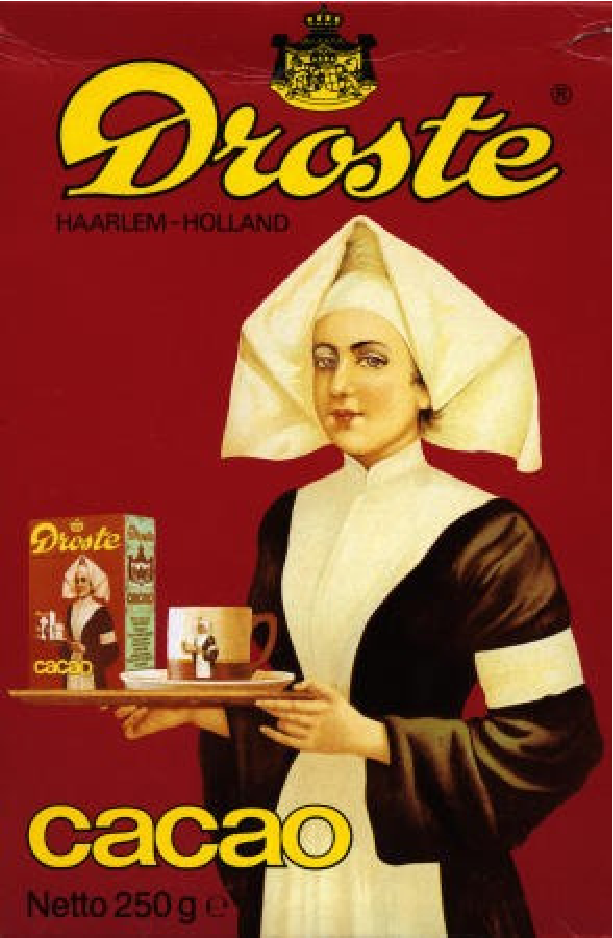
\includegraphics[width=0.38\textwidth]{graficos/droste}
%  \end{center}
%  \caption{\small Una imagen recursiva: la publicidad de Cacao Droste,
%bajada de \url{http://en.wikipedia.org/wiki/Image:Droste.jpg}}
%  \vspace{-3cm}
%\end{wrapfigure}

Estamos acostumbrados a escribir funciones que llaman a otras funciones.
Pero lo cierto es que nada impide que en Python (y en muchos otros
lenguajes) una función se llame a sí misma. Y lo más interesante es que
esta propiedad, que se llama {\it recursión}, permite en muchos casos
encontrar soluciones muy elegantes para determinados problemas. \\

En materias de matemática se estudian los razonamientos por inducción para
probar propiedades de números enteros, la recursión no es más que una
generalización de la inducción a más estructuras: las listas, las cadenas
de caracteres, las funciones, etc.

\begin{figure}
  \begin{center}
    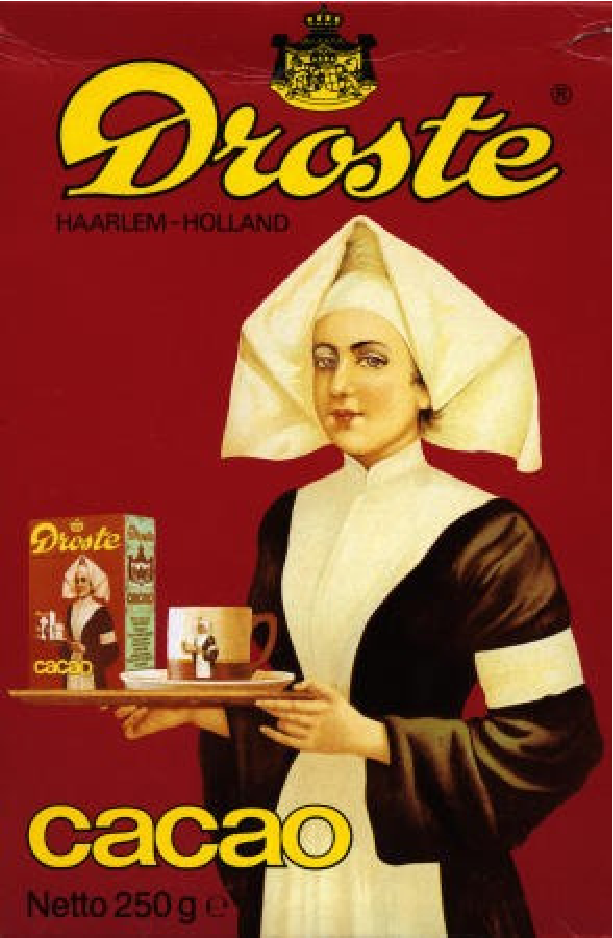
\includegraphics[width=0.38\textwidth]{graficos/droste}
  \end{center}
  \caption{\small Una imagen recursiva: la publicidad de Cacao Droste,
bajada de \url{http://en.wikipedia.org/wiki/Image:Droste.jpg}}
\end{figure}

A continuación estudiaremos diversas situaciones en las cuales aparece la
recursión, veremos cómo es que esto puede funcionar, algunas situaciones en
las que es conveniente utilizarla y otras situaciones en las que no.

% TODO: más que dejar lugar, habría que escribir algo más.
%\vspace{2.5cm}

\section{Una función recursiva matemática}

Es muy común tener definiciones inductivas de operaciones, como por ejemplo:

$x! = x * (x-1)!$ si $x>0$, $0! = 1$

Este tipo de definición se traduce naturalmente en una función en Python:

\begin{codigo-python-sn}
def factorial(n):
    """ Precondición: n entero >=0
        Devuelve: n! """
    if n == 0:
        return 1

    return n * factorial(n-1)
\end{codigo-python-sn}

Esta es la ejecución del factorial para \lstinline!n=0! y para
\lstinline!n=3!.

\begin{codigo-python-sn}
>>> factorial(0)
1
>>> factorial(3)
6
\end{codigo-python-sn}

El sentido de la instrucción de la instrucción
\lstinline|n * factorial (n-1)| es exactamente el mismo que el de la
definición inductiva: para calcular el factorial de $n$ se debe multiplicar
$n$ por el factorial de $n-1$.

Dos piezas fundamentales para garantizar el funcionamiento de este programa
son:

\begin{itemize}
\item Que se defina un {\it caso base} (en este caso la indicación, no recursiva,
de cómo calcular \lstinline|factorial(0)|), que corta las llamadas recursivas.

\item Que el argumento de la función respete la precondición
de que \lstinline!n! debe ser {\it un entero mayor o igual que 0}.
\end{itemize}

Dado que ya vimos la pila de evaluación, y cómo funciona, no debería
llamarnos la atención que esto pueda funcionar adecuadamente en un lenguaje
de programación que utilice pila para evaluar.

Para poder analizar qué sucede a cada paso de la ejecución de la función,
utilizaremos una versión más detallada del mismo código, en la que cada
paso se asigna a una variable.

\begin{codigo-python-sn}
def factorial(n):
    """ Precondición: n entero >=0
        Devuelve: n! """
    if n == 0:
        r = 1
        return r

    f = factorial(n-1)
    r = n * f
    return r
\end{codigo-python-sn}

Esta porción de código funciona exactamente igual que la anterior, pero nos
permite ponerles nombres a los resultados intermedios de cada operación
para poder estudiar qué sucede a cada paso.
Analicemos, entonces, el \lstinline|factorial(3)|  mediante la pila de
evaluación:

\begin{enumerate}

\item  \verb|factorial(3)              |
	\begin{tabular}{r|r|}
	\hline
	\verb|factorial|&n $\rightarrow$3\\
	\hline
	\end{tabular}

\item  \verb|if n == 0:                |
	\begin{tabular}{r|r|}
	\hline
	\verb|factorial|&n $\rightarrow$3\\
	\hline
	\end{tabular}

\item  \verb|f = factorial (n-1)       |
	\begin{tabular}{r|r|}
	\hline
	\verb|factorial|&n $\rightarrow$3\\
	\hline
	\end{tabular}
	\begin{tabular}{l}
	Se suspende el cálculo. \\
	Se llama a \verb|factorial(2)|.
	\end{tabular}

\item  \verb|factorial(2)              |
	\begin{tabular}{r|r|}
	\hline
	\verb|factorial|&n $\rightarrow$2\\
	\hline
	\hline
	\verb|factorial|&n $\rightarrow$3\\
	\hline
	\end{tabular}

\item  \verb|if n == 0:                |
	\begin{tabular}{r|r|}
	\hline
	\verb|factorial|&n $\rightarrow$2\\
	\hline
	\hline
	\verb|factorial|&n $\rightarrow$3\\
	\hline
	\end{tabular}

\item  \verb|f = factorial (n-1)       |
	\begin{tabular}{r|r|}
	\hline
	\verb|factorial|&n $\rightarrow$2\\
	\hline
	\hline
	\verb|factorial|&n $\rightarrow$3\\
	\hline
	\end{tabular}
	\begin{tabular}{l}
	Se suspende el cálculo. \\
	Se llama a \verb|factorial(1)|.
	\end{tabular}

\item  \verb|factorial(1)              |
	\begin{tabular}{r|r|}
	\hline
	\verb|factorial|&n $\rightarrow$1\\
	\hline
	\hline
	\verb|factorial|&n $\rightarrow$2\\
	\hline
	\hline
	\verb|factorial|&n $\rightarrow$3\\
	\hline
	\end{tabular}

\item  \verb|if n == 0:                |
	\begin{tabular}{r|r|}
	\hline
	\verb|factorial|&n $\rightarrow$1\\
	\hline
	\hline
	\verb|factorial|&n $\rightarrow$2\\
	\hline
	\hline
	\verb|factorial|&n $\rightarrow$3\\
	\hline
	\end{tabular}

\item  \verb|f = factorial (n-1)       |
	\begin{tabular}{r|r|}
	\hline
	\verb|factorial|&n $\rightarrow$1\\
	\hline
	\hline
	\verb|factorial|&n $\rightarrow$2\\
	\hline
	\hline
	\verb|factorial|&n $\rightarrow$3\\
	\hline
	\end{tabular}
	\begin{tabular}{l}
	Se suspende el cálculo. \\
	Se llama a \verb|factorial(0)|.
	\end{tabular}

\item  \verb|factorial(0)              |
	\begin{tabular}{r|r|}
	\hline
	\verb|factorial|&n $\rightarrow$0\\
	\hline
	\hline
	\verb|factorial|&n $\rightarrow$1\\
	\hline
	\hline
	\verb|factorial|&n $\rightarrow$2\\
	\hline
	\hline
	\verb|factorial|&n $\rightarrow$3\\
	\hline
	\end{tabular}

\item  \verb|if n == 0:                |
	\begin{tabular}{r|r|}
	\hline
	\verb|factorial|&n $\rightarrow$0\\
	\hline
	\hline
	\verb|factorial|&n $\rightarrow$1\\
	\hline
	\hline
	\verb|factorial|&n $\rightarrow$2\\
	\hline
	\hline
	\verb|factorial|&n $\rightarrow$3\\
	\hline
	\end{tabular}

\item  \verb|r = 1                     |
	\begin{tabular}{r|r|}
	\hline
	\verb|factorial|&n $\rightarrow$0\\
	          &r $\rightarrow$1\\
	\hline
	\hline
	\verb|factorial|&n $\rightarrow$1\\
	\hline
	\hline
	\verb|factorial|&n $\rightarrow$2\\
	\hline
	\hline
	\verb|factorial|&n $\rightarrow$3\\
	\hline
	\end{tabular}

\item
\begin{tabular}{l}
En \lstinline!factorial(0)!: \\ \verb|    return r| \\
En \lstinline!factorial(1)!: \\ \verb|    f = factorial (n-1) |
\end{tabular}
	\begin{tabular}{r|r|}
	\hline
	\verb|factorial|&n $\rightarrow$1\\
	&f $\rightarrow$1\\
	\hline
	\hline
	\verb|factorial|&n $\rightarrow$2\\
	\hline
	\hline
	\verb|factorial|&n $\rightarrow$3\\
	\hline
	\end{tabular}

\item  \verb|r = n * f                 |
\begin{tabular}{r|r|}
\hline
\verb|factorial|&n $\rightarrow$1\\
  &f $\rightarrow$1\\
  &r $\rightarrow$1\\
\hline
\hline
\verb|factorial|&n $\rightarrow$2\\
\hline
\hline
\verb|factorial|&n $\rightarrow$3\\
\hline
\end{tabular}

\item
\begin{tabular}{l}
En \lstinline!factorial(1)!: \\ \verb|    return r| \\
En \lstinline!factorial(2)!: \\ \verb|    f = factorial (n-1) |
\end{tabular}
	\begin{tabular}{r|r|}
	\hline
	\verb|factorial|&n $\rightarrow$2\\
	&f $\rightarrow$1\\
	\hline
	\hline
	\verb|factorial|&n $\rightarrow$3\\
	\hline
	\end{tabular}

\item  \verb|r = n * f                 |
	\begin{tabular}{r|r|}
	\hline
	\verb|factorial|&n $\rightarrow$2\\
	  &f $\rightarrow$1\\
	  &r $\rightarrow$2\\
	\hline
	\hline
	\verb|factorial|&n $\rightarrow$3\\
	\hline
	\end{tabular}

\item
\begin{tabular}{l}
En \lstinline!factorial(2)!: \\ \verb|    return r| \\
En \lstinline!factorial(3)!: \\ \verb|    f = factorial (n-1) |
\end{tabular}
	\begin{tabular}{r|r|}
	\hline
	\verb|factorial|&n $\rightarrow$3\\
	&f $\rightarrow$2\\
	\hline
	\end{tabular}

\item  \verb|r = n * f                 |
	\begin{tabular}{r|r|}
	\hline
	\verb|factorial|&n $\rightarrow$3\\
	  &f $\rightarrow$2\\
	  &r $\rightarrow$6\\
	\hline
	\end{tabular}

\item  \verb|return r                  |
	\begin{tabular}{r|r|}
	\hline
	\verb!    ! pila vacía \verb!   ! \\
	\hline
	\end{tabular}
	\hspace{0.2cm} Devuelve el valor $6$
\end{enumerate}

\begin{minipage}{\linewidth}
\centering%
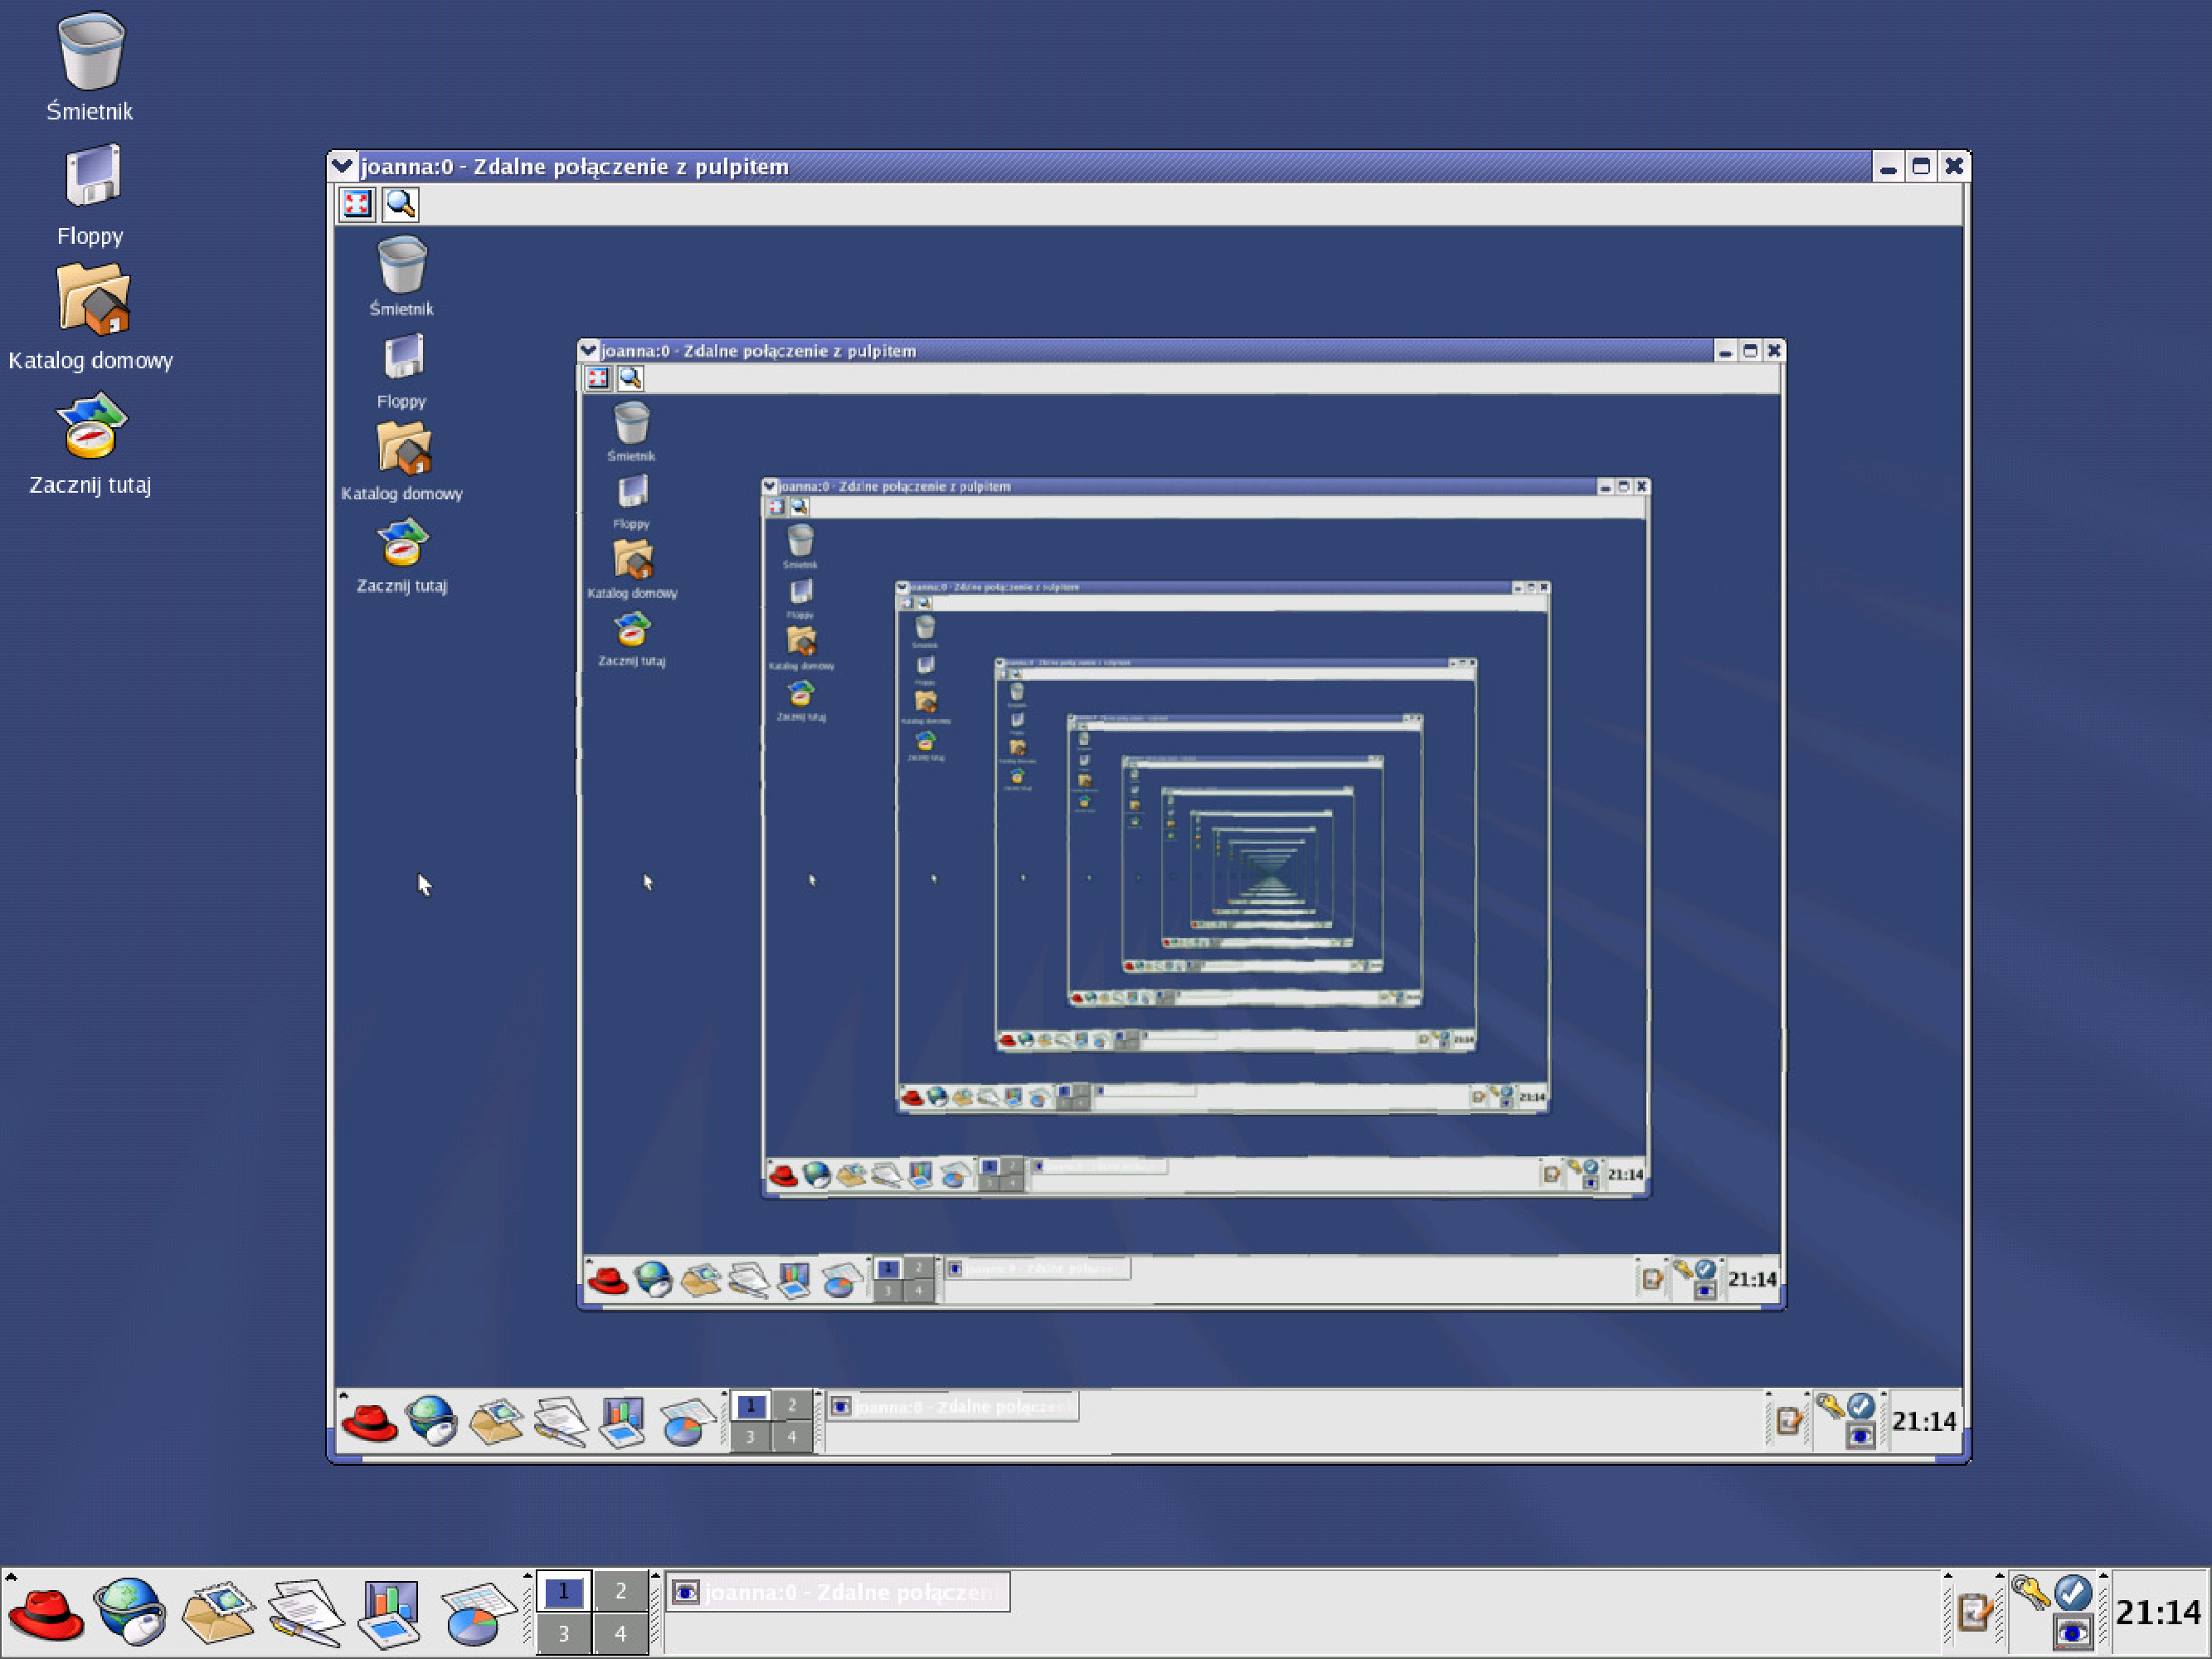
\includegraphics[width=10cm]{graficos/recursive}
\figcaption{Otra imagen recursiva: captura de pantalla de RedHat, bajada de http://www.jfedor.org/}%
\label{fig:redhat_recursivo}%
\end{minipage}

\section{Algoritmos recursivos y algoritmos iterativos}

Llamaremos {\it algoritmos recursivos} a aquellos que realizan llamadas
recursivas para llegar al resultado, y {\it algoritmos iterativos} a
aquellos que llegan a un resultado a través de una iteración mediante un
ciclo definido o indefinido.

Todo algoritmo recursivo puede expresarse como iterativo y viceversa.  Sin
embargo, según las condiciones del problema a resolver podrá ser preferible
utilizar la solución recursiva o la iterativa.

Una posible implementación iterativa de la función \lstinline!factorial!
vista anteriormente sería:

\begin{codigo-python-sn}
def factorial(n):
    """ Precondición: n entero >=0
        Devuelve: n! """

    fact = 1
    for num in xrange(n, 1, -1):
        fact *= num
    return fact
\end{codigo-python-sn}

Se puede ver que en este caso no es necesario incluir un caso base, ya que
el mismo ciclo incluye una condición de corte, pero que sí es necesario
incluir un acumulador, que en el caso recursivo no era necesario.

Por otro lado, si hiciéramos el seguimiento de esta función, como se hizo
para la versión recursiva, veríamos que se trata de una única pila, en la
cual se van modificando los valores de \lstinline!num! y \lstinline!fact!.

Es por esto que las versiones recursivas de los algoritmos, en general,
utilizan más memoria (la pila del estado de las funciones se guarda en
memoria) pero suelen ser más elegantes.

\section{Un ejemplo de recursividad elegante}

Consideremos ahora otro problema que puede ser resuelto de forma elegante
mediante un algoritmo recursivo.

La función \lstinline!potencia(b,n)!, vista en unidades anteriores,
realizaba \lstinline!n! iteraciones para poder obtener el valor de $b^n$.
Sin embargo, es posible optimizarla teniendo en cuenta que: \\

\begin{tabular}{ll}
$b^n = b^{n/2} \times b^{n/2}$ & Si $n$ es par. \\
$b^n = b^{(n-1)/2} \times b^{(n-1)/2} \times b$ &  Si $n$ es impar. \\
\end{tabular} \\

Antes de programar cualquier función recursiva es necesario decidir cuál
será el {\it caso base} y cuál el {\it caso recursivo}.  Para esta función,
tomaremos $n=0$ como el caso base, en el que devolveremos $1$; y el caso
recursivo tendrá dos partes, correspondientes a los dos posibles grupos de
valores de $n$.

\begin{codigo-python-sn}
def potencia(b,n):
    """ Precondición: n debe ser mayor o igual que cero.
        Devuelve: b^n. """

    # Caso base
    if n <= 0:
        return 1

    # n par
    if n % 2 == 0:
        pot = potencia(b, n/2)
        return pot * pot
    # n impar
    else:
        pot = potencia(b, (n-1)/2)
        return pot * pot * b
\end{codigo-python-sn}

El uso de la variable \lstinline!pot! en este caso no es optativo, ya que
es una de las ventajas principales de esta implementación: se aprovecha el
resultado calculado en lugar de tener que calcularlo dos veces. Vemos que
este código funciona correctamente:

\begin{codigo-python-sn}
>>> potencia(2,10)
1024
>>> potencia(3,3)
27
>>> potencia(5,0)
1
\end{codigo-python-sn}

El orden de las llamadas, haciendo un seguimiento simplificado de la
función será:

\begin{enumerate}
\item \verb!potencia(2,10)!
\item \hspace{1cm} \verb!pot = potencia(2,5) !
\hspace{4cm} \begin{tabular}{|c|c|}b $\rightarrow$ 2 & n $\rightarrow$ 10\end{tabular}
\item \hspace{2cm} \verb!pot = potencia(2,2) !
\hspace{3cm} \begin{tabular}{|c|c|}b $\rightarrow$ 2 & n $\rightarrow$ 5$\;\,$\end{tabular}
\item \hspace{3cm} \verb!pot = potencia(2,1) !
\hspace{2cm} \begin{tabular}{|c|c|}b $\rightarrow$ 2 & n $\rightarrow$ 2$\;\,$\end{tabular}
\item \hspace{4cm} \verb!pot = potencia(2,0) !
\hspace{1cm} \begin{tabular}{|c|c|}b $\rightarrow$ 2 & n $\rightarrow$ 1$\;\,$\end{tabular}
\item \hspace{5cm} \verb!return 1            !
\hspace{0cm} \begin{tabular}{|c|c|}b $\rightarrow$ 2 & n $\rightarrow$ 0$\;\,$\end{tabular}
\item \hspace{4cm} \verb!return 1 * 1 * 2    !
\hspace{1cm} \begin{tabular}{|c|c|c|}b $\rightarrow$ 2 & n $\rightarrow$ 1$\;\,$
& pot $\rightarrow$ 1$\;\,$ \end{tabular}
\item \hspace{3cm} \verb!return 2 * 2        !
\hspace{2cm} \begin{tabular}{|c|c|c|}b $\rightarrow$ 2 & n $\rightarrow$ 2$\;\,$
& pot $\rightarrow$ 2$\;\,$ \end{tabular}
\item \hspace{2cm} \verb!return 4 * 4 * 2    !
\hspace{3cm} \begin{tabular}{|c|c|c|}b $\rightarrow$ 2 & n $\rightarrow$ 5$\;\,$
& pot $\rightarrow$ 4$\;\,$ \end{tabular}
\item \hspace{1cm} \verb!return 32 * 32      !
\hspace{4cm} \begin{tabular}{|c|c|c|}b $\rightarrow$ 2 & n $\rightarrow$ 10
& pot $\rightarrow$ 32 \end{tabular}
\end{enumerate}

Se puede ver, entonces, que para calcular $2^{10}$ se realizaron 5 llamadas a
\lstinline!potencia!, mientras que en la implementación más sencilla se
realizaban 10 iteraciones. Y esta optimización será cada vez más importante
a medida que aumenta \lstinline!n!, por ejemplo, para $n = 100$ se
realizarán 8 llamadas recursivas, para $n = 1000$, 11 llamadas. \\

% Esto no es para darlo, es sólo para que esté

Para transformar este algoritmo recursivo en un algoritmo iterativo, es
necesario {\it simular} la pila de llamadas a funciones mediante una pila que
almacene los valores que sean necesarios.  En este caso, lo que apilaremos será
si el valor de \lstinline!n! es par o no.

\begin{codigo-python-sn}
def potencia(b,n):
    """ Precondición: n debe ser mayor o igual que cero.
        Devuelve: b^n. """

    pila = []
    while n > 0:
        if n % 2 == 0:
            pila.append(True)
            n /= 2
        else:
            pila.append(False)
            n = (n-1)/2

    pot = 1
    while pila:
        es_par = pila.pop()
        if es_par:
            pot = pot * pot
        else:
            pot = pot * pot * b

    return pot
\end{codigo-python-sn}

Como se puede ver, este código es mucho más complejo que la versión recursiva,
esto se debe a que utilizando recursividad el uso de la pila de llamadas a
funciones oculta el proceso de apilado y desapilado y permite concentrarse
en la parte importante del algoritmo.

\section{Un ejemplo de recursividad poco eficiente}

Del ejemplo anterior se podría deducir que siempre es mejor utilizar algoritmos
recursivos, sin embargo -como ya se dijo- cada situación debe ser analizada por
separado.

Un ejemplo clásico en el cual la recursividad tiene un resultado muy poco
eficiente es el de los números de fibonacci.  La sucesión de fibonacci está
definida por la siguiente relación:

\begin{tabular}{rcl}
\lstinline!fib(0)! &=& 0 \\
\lstinline!fib(1)! &=& 1 \\
\lstinline!fib(n)! &=& \lstinline!fib(n-1)! + \lstinline!fib(n-2)!
\end{tabular}

Los primeros números de esta sucesión son: $0$, $1$, $1$, $2$, $3$, $5$, $8$,
$13$, $21$, $34$, $55$.

Dada la definición recursiva de la sucesión, puede resultar muy tentador
escribir una función que calcule en valor de \lstinline!fib(n)! de la siguiente
forma:

\begin{codigo-python-sn}
def fib(n):
    """ Precondición: n debe ser >= 0.
        Devuelve: el número de fibonacci número n. """
    if n == 0 or n == 1:
        return n
    return fib(n-1) + fib(n-2)
\end{codigo-python-sn}

Sin embargo, si bien es muy sencillo y elegante, este código es extremadamente
poco eficiente.  Ya que para calcular \lstinline!fib(n-1)! es necesario calcular
\lstinline!fib(n-2)!, que luego volverá a ser calculado para obtener el valor de
\lstinline!fib(n)!.

Por ejemplo, una simple llamada a \lstinline!fib(5)!, generaría
recursivamente todas las llamadas ilustradas en la Figura \ref{fibonacci}.
Puede verse que muchas de estas llamadas están repetidas, generando un
total de 15 llamadas a la función \lstinline!fib!, sólo para devolver el
número 5.

\begin{figure}[htb]
\includegraphics{graficos/18_fibonacci}
\caption{Árbol de llamadas para \lstinline!fib(5)!}
\label{fibonacci}
\end{figure}

En este caso, será mucho más conveniente utilizar una versión iterativa,
que vaya almacenando los valores de las dos variables anteriores a medida
que los va calculando.

% FIXME: hace falta un newpage, porque sino corta el código mal
\newpage

\begin{codigo-python-sn}
def fib(n):
    """ Precondición: n debe ser >= 0.
        Devuelve: el número de fibonacci número n. """
    if n == 0 or n == 1:
        return n

    ant2 = 0
    ant1 = 1
    for i in xrange(2, n+1):
        fibn = ant1 + ant2
        ant2 = ant1
        ant1 = fibn
    return fibn
\end{codigo-python-sn}

Vemos que el caso base es el mismo para ambos algoritmos, pero que en el
caso iterativo se calcula el número de fibonacci de forma incremental, de
modo que para obtener el valor de \lstinline!fib(n)! se harán $n-1$
iteraciones.

\begin{atencion}
En definitiva, vemos que un algoritmo recursivo {\bf no} es mejor que uno
iterativo, ni viceversa.  En cada situación será conveniente analizar cuál
algoritmo provee la solución al problema de forma más clara y eficiente.
\end{atencion}

\section{Limitaciones}

Si creamos una función sin {\it caso base}, obtendremos el equivalente
recursivo de un bucle infinito.  Sin embargo, como cada llamada recursiva
agrega un elemento a la pila de llamadas a funciones y la memoria de
nuestras computadoras no es infinita, el ciclo deberá terminarse cuando se
agote la memoria disponible.

En particular, en Python, para evitar que la memoria se termine, la pila de
ejecución de funciones tiene un límite. Es decir, que si se ejecuta un
código como el que sigue:

\begin{codigo-python-sn}
def inutil(n):
    return inutil(n-1)
\end{codigo-python-sn}

Se obtendrá un resultado como el siguiente:

\begin{codigo-python-sn}
>>> inutil(1)
  File "<stdin>", line 2, in inutil
  File "<stdin>", line 2, in inutil
  (...)
  File "<stdin>", line 2, in inutil
RuntimeError: maximum recursion depth exceeded
\end{codigo-python-sn}

El límite por omisión es de 1000 llamadas recursivas. Es posible modificar
el tamaño máximo de la pila de recursión mediante la instrucción
\lstinline!sys.setrecursionlimit(n)!.  Sin embargo, si se está alcanzando
este límite suele ser una buena idea pensar si realmente el algoritmo
recursivo es el que mejor resuelve el problema.

\begin{sabias_que}
Existen algunos lenguajes {\it funcionales}, como Haskell, ML, o Scheme, en
los cuales la recursividad es la única forma de realizar un ciclo.  Es
decir, no existen construcciones {\tt while} ni {\tt for}.

Estos lenguajes cuentan con una optimización especial, llamada {\it
optimización de recursión por cola} ({\it tail recursion optimization}),
que permite que cuando una función realiza su llamada recursiva como {\bf
última} acción antes de terminar, no se apile el estado de la función
innecesariamente, evitando el consumo adicional de memoria mencionado
anteriormente.

La función \lstinline!factorial! vista en esta unidad es un ejemplo de {\it
recursión por cola} cuya ejecución puede ser optimizada por el compilador o
intérprete del lenguaje.
\end{sabias_que}

\section{Resumen}

\begin{itemize}

\item A medida que se realizan llamadas a funciones, el estado de las
funciones anteriores se almacena en una {\it pila} de llamadas a funciones.

\item Esto permite que sea posible que una función se llame a sí misma,
pero que las variables dentro de la función tomen distintos valores.

\item La {\bf recursión} es el proceso en el cual una función se llama a
sí misma.  Este proceso permite crear un nuevo tipo de ciclos.

\item Siempre que se escribe una función recursiva es importante considerar
el {\bf caso base} (el que detendrá la recursividad) y el {\bf caso
recursivo} (el que realizará la llamada recursiva).  Una función recursiva
sin caso base, es equivalente a un bucle infinito.

\item Una función no es mejor ni peor por ser recursiva.  En cada situación
a resolver puede ser conveniente utilizar una solución recursiva o una
iterativa.  Para elegir una o la otra será necesario analizar las
características de elegancia y eficiencia.

\end{itemize}


\newpage
\section{Ejercicios}

\extractionlabel{guia}
\begin{ejercicio}
Escribir una función que reciba un número positivo $n$ y devuelva
la cantidad de dígitos que tiene.
\end{ejercicio}

\extractionlabel{guia}
\begin{ejercicio}
Escribir una función que simule el siguiente experimento:
Se tiene una rata en una jaula con 3 caminos, entre los cuales elige
al azar (cada uno tiene la misma probabilidad), si elige el {\it 1} luego
de 3 minutos vuelve a la jaula, si elige el {\it 2} luego de 5 minutos vuelve a
la jaula, en el caso de elegir el {\it 3} luego de 7 minutos sale de la jaula.
La rata no aprende, siempre elige entre los 3 caminos con la misma probabilidad,
pero quiere su libertad, por lo que recorrerá los caminos hasta salir de la jaula.

La función debe devolver el tiempo que tarda la rata en salir de la jaula.
\end{ejercicio}

\extractionlabel{guia}
\begin{ejercicio}
Escribir una función que reciba 2 enteros {\it n} y {\it b} y devuelva
\verb!True! si {\it n} es potencia de {\it b}.

Ejemplos:
\begin{verbatim}
>>> es_potencia(8,2)
True
>>> es_potencia(64,4)
True
>>> es_potencia(70,10)
False
\end{verbatim}
\end{ejercicio}

\extractionlabel{guia}
\begin{ejercicio}
Escribir una funcion recursiva que reciba como parámetros dos strings {\it a} y
{\it b}, y devuelva una lista con las posiciones en donde se encuentra {\it b}
dentro de {\it a}.

Ejemplo:
\begin{verbatim}
>>> posiciones_de("Un tete a tete con Tete", "te")
[3, 5, 10, 12, 21]
\end{verbatim}
\end{ejercicio}

\extractionlabel{guia}
\begin{ejercicio}
Escribir dos funciones mutualmente recursivas par(n) e impar(n) que
determinen la paridad del numero natural dado, conociendo solo que:
\begin{itemize}
    \item 1 es impar.
    \item Si un número es impar, su antecesor es par; y viceversa.
\end{itemize}
\end{ejercicio}

\extractionlabel{guia}
\begin{ejercicio}
Escribir una función que calcule recursivamente el n-ésimo número
triangular (el número 1 + 2 + 3 + ... + n).
\end{ejercicio}

\extractionlabel{guia}
\begin{ejercicio}
Escribir una función que calcule recursivamente cuántos elementos
hay en una pila, suponiendo que la pila sólo tiene los métodos apilar
y desapilar, y no altere el contenido de la pila.\\
¿Implementarías esta función para un programa real? ¿Por qué?
\end{ejercicio}

\extractionlabel{guia}
\begin{ejercicio}
Escribir una funcion recursiva que encuentre el mayor elemento de una lista.
\end{ejercicio}

\extractionlabel{guia}
\begin{ejercicio}
Escribir una función recursiva para replicar los elementos de una lista
una cantidad n de veces. Por ejemplo,
\verb!replicar ([1, 3, 3, 7], 2) = ([1, 1, 3, 3, 3, 3, 7, 7])!
\end{ejercicio}


% Copyright (C) 2008-2010 Rosita Wachenchauzer <rositaw@gmail.com>
%               Margarita Manterola <margamanterola@gmail.com>

% Esta obra está licenciada de forma dual, bajo las licencias Creative
% Commons:
%  * Atribución-Compartir Obras Derivadas Igual 2.5 Argentina
%    http://creativecommons.org/licenses/by-sa/2.5/ar/
%  * Atribución-Compartir Obras Derivadas Igual 3.0 Unported
%    http://creativecommons.org/licenses/by-sa/3.0/deed.es_AR.
%
% A su criterio, puede utilizar una u otra licencia, o las dos.
% Para ver una copia de las licencias, puede visitar los sitios
% mencionados, o enviar una carta a Creative Commons,
% 171 Second Street, Suite 300, San Francisco, California, 94105, USA.

\chapter{Ordenar listas}

Al estudiar las listas de Python, vimos que poseen un método \lstinline!sort!
que las ordena de menor a mayor de acuerdo a una clave (e incluso de acuerdo a
una relación de orden que se desee, dada a través del parámetro
\lstinline!cmp!).

Sin embargo, no todas las estructuras cuentan con un método
\lstinline!sort! que las ordene.  Es por ello que en esta unidad nos
plantearemos cómo se hace para ordenar cuando no hay un método
\lstinline!sort!, y cuánto cuesta ordenar.

Ante todo una advertencia: hay varias maneras de ordenar, y no todas
cuestan lo mismo. Vamos a empezar viendo las más sencillas de escribir
(que en general suelen ser las más caras).

\section{Ordenamiento por selección}
Éste método de ordenamiento se basa en la siguiente idea:

\begin{itemize}

\item {\bf Paso 1.1}: Buscar el mayor de todos los elementos de la lista.
\\

\hspace{0.75cm}
\begin{tabular}[c]{|c|c|c|c|c|c|}
\hline
3& 2&-1&5&0&2\\
\hline
\end{tabular}
\hspace{0.75cm}
\begin{tabular}{p{9cm}}
Encuentra el valor $5$ en la posición $3$.
\end{tabular}\\

\item {\bf Paso 1.2}: Poner el mayor al final (intercambiar el que está en la última
posición de la lista con el mayor encontrado).\\

\hspace{0.75cm}
\begin{tabular}[c]{|c|c|c|c|c|c|}
\hline
3& 2&-1&2&0&5\\
\hline
\end{tabular}
\hspace{0.75cm}
\begin{tabular}{p{9cm}}
Intercambia el elemento de la posición $3$ con el de la posición $5$. \\
{\it En la última posición de la lista está el mayor de todos.}
\end{tabular} \\

\item {\bf Paso 2.1}: Buscar el mayor de todos los elementos del segmento de la lista
entre la primera y la anteúltima posición. \\

\hspace{0.75cm}
\begin{tabular}[c]{|c|c|c|c|c|c|}
\hline
3& 2&-1&2&0&5\\
\hline
\end{tabular}
\hspace{0.75cm}
\begin{tabular}{p{9cm}}
Encuentra el valor $3$ en la posición $0$.
\end{tabular} \\

\item {\bf Paso 2.2}: Poner el mayor al final del segmento (intercambiar el que está en la última
posición del segmento --o sea anteúltima posición de la lista-- con el mayor encontrado). \\

\hspace{0.75cm}
\begin{tabular}[c]{|c|c|c|c|c|c|}
\hline
0& 2&-1&2&3&5\\
\hline
\end{tabular}
\hspace{0.75cm}
\begin{tabular}{p{9cm}}
Intercambia el elemento de la posición $0$ con el valor de la posición $4$. \\
{\it En la anteúltima y última posición de la lista están los dos mayores en su posición definitiva.}
\end{tabular} \\

$\dots$\\

\item {\bf Paso n}: Se termina cuando queda un único elemento sin tratar: el que está
en la primera posición de la lista, y que es el menor de todos porque todos los
mayores fueron reubicados. \\

\hspace{0.75cm}
\begin{tabular}[c]{|c|c|c|c|c|c|}
\hline
-1& 0&2&2&3&5\\
\hline
\end{tabular}
\hspace{0.75cm}
\begin{tabular}{p{9cm}}
{\it La lista se encuentra ordenada}.
\end{tabular}\\
\end{itemize}

\begin{codigo}{seleccion.py}{Ordena una lista por selección}
\label{ord_seleccion}
\lstinputlisting{src/19_ordenamiento/seleccion.py}
\end{codigo}

La implementación en Python puede verse en el Código \ref{ord_seleccion}.


La función principal, \lstinline!ord_seleccion! es la encargada de recorrer
la lista, ubicando el mayor elemento al final del segmento y luego
reduciendo el segmento a analizar.

Mientras que \lstinline!buscar_max! es una función que ya se estudió
previamente, que busca el mayor elemento de la lista y devuelve su
posición.

A continuación, algunas una ejecuciones de prueba de ese código:

\begin{codigo-python-sn}
>>> l=[3, 2, -1, 5, 0, 2]
>>> ord_seleccion(l)
DEBUG:  3 5 [3, 2, -1, 2, 0, 5]
DEBUG:  0 4 [0, 2, -1, 2, 3, 5]
DEBUG:  1 3 [0, 2, -1, 2, 3, 5]
DEBUG:  1 2 [0, -1, 2, 2, 3, 5]
DEBUG:  0 1 [-1, 0, 2, 2, 3, 5]
>>> print l
[-1, 0, 2, 2, 3, 5]
>>> l=[]
>>> ord_seleccion(l)
>>> l=[1]
>>> ord_seleccion(l)
>>> print l
[1]
>>> l=[1,2,3,4,5]
>>> ord_seleccion(l)
DEBUG:  4 4 [1, 2, 3, 4, 5]
DEBUG:  3 3 [1, 2, 3, 4, 5]
DEBUG:  2 2 [1, 2, 3, 4, 5]
DEBUG:  1 1 [1, 2, 3, 4, 5]
\end{codigo-python-sn}

Puede verse que aún cuando la lista está ordenada, se la recorre buscando
los mayores elementos y ubicándolos en la misma posición en la que se
encuentran.

\subsection{Invariante en el ordenamiento por selección}

Todo ordenamiento tiene un invariante que permite asegurarse de que cada
paso que se toma va en la dirección de obtener una lista ordenada.

En el caso del ordenamiento por selección, el invariante es que los
elementos desde \lstinline!n+1! hasta el final de la lista están ordenados y
son mayores que los elementos de \lstinline!0! a \lstinline!n!, es decir
que ya están en su posición definitiva.

\subsection{¿Cuánto cuesta ordenar por selección?}

Como se puede ver en el código de la función \lstinline!buscar_max!, para
buscar el máximo elemento en un segmento de lista se debe recorrer todo ese
segmento, por lo que en nuestro caso debemos recorrer en el primer paso $N$
elementos, en el segundo paso $N-1$ elementos, en el tercer paso $N-2$
elementos, etc. Cada visita a un elemento implica una cantidad constante y
pequeña de comparaciones (que no depende de $N$). Por lo tanto tenemos que

\begin{equation}
T(N) \approx c * (2 + 3 + \ldots + N) \approx c * N * (N+1)/2 \sim N^2
\end{equation}

O sea que ordenar por selección una lista de tamaño $N$ insume tiempo del
orden de $N^2$.  Como ya se vio, este tiempo es independiente de si la
lista estaba previamente ordenda o no.

En cuanto al espacio utilizado, sólo se tiene en memoria la
lista que se desea ordenar y algunas variables de tamaño 1.

\section{Ordenamiento por inserción}

Éste otro método de ordenamiento se basa en la siguiente idea:

\begin{itemize}

\item {\bf Paso 0}: Partimos de la misma lista de ejemplo utilizada para el ordenamiento
por selección. \\

\hspace{0.75cm}
\begin{tabular}[c]{|c|c|c|c|c|c|}
\hline
3& 2&-1&5&0&2\\
\hline
\end{tabular}
\hspace{0.75cm}

\item {\bf Paso 1}: Considerar el segundo elemento de la lista,
y ordenarlo respecto del primero, deplazándolo hasta la
posición correcta, si corresponde. \\

\hspace{0.75cm}
\begin{tabular}[c]{|c|c|c|c|c|c|}
\hline
2& 3&-1&5&0&2\\
\hline
\end{tabular}
\hspace{0.75cm}
\begin{tabular}{p{9cm}}
Se desplaza el valor $2$ antes de $3$.
\end{tabular}

\item {\bf Paso 2}: Considerar el tercer elemento de la lista,
y ordenarlo respecto del primero y el segundo, deplazándolo hasta la
posición correcta, si corresponde. \\

\hspace{0.75cm}
\begin{tabular}[c]{|c|c|c|c|c|c|}
\hline
-1& 2&3&5&0&2\\
\hline
\end{tabular}
\hspace{0.75cm}
\begin{tabular}{p{9cm}}
Se desplaza el valor $-1$ antes de $2$ y de $3$.
\end{tabular}

\item {\bf Paso 3}: Considerar el cuarto elemento de la lista,
y ordenarlo respecto del primero, el segundo y el tercero, deplazándolo hasta la
posición correcta, si corresponde. \\

\hspace{0.75cm}
\begin{tabular}[c]{|c|c|c|c|c|c|}
\hline
-1& 2&3&5&0&2\\
\hline
\end{tabular}
\hspace{0.75cm}
\begin{tabular}{p{9cm}}
El $5$ está correctamente ubicado respecto de $-1$,$2$ y $3$ (como el segmento
hasta la tercera posición está ordenado, basta con comparar con el tercer elemento del
segmento para verificarlo).\\
\end{tabular}

$\dots$\\

\item {\bf Paso N-1}: \\

\hspace{0.75cm}
\begin{tabular}[c]{|c|c|c|c|c|c|}
\hline
-1& 0&2&3&5&2\\
\hline
\end{tabular}
\hspace{0.75cm}
\begin{tabular}{p{9cm}}
Todos los elementos excepto el ante-último ya se encuentran ordenados.
\end{tabular}

\item {\bf Paso N}:
Considerar el $N$--ésimo elemento de la lista, y ordenarlo respecto del
segmento formado por el primero hasta el $N-1$--ésimo, deplazándolo hasta
la posición correcta, si corresponde. \\

\hspace{0.75cm}
\begin{tabular}[c]{|c|c|c|c|c|c|}
\hline
-1& 0&2&2&3&5\\
\hline
\end{tabular}
\hspace{0.75cm}
\begin{tabular}{p{9cm}}
Se desplaza el valor $2$ antes de $3$ y de $5$.
\end{tabular}

\end{itemize}

\begin{codigo}{insercion.py}{Ordena una lista por Inserción}
\label{ord_insercion}
\lstinputlisting{src/19_ordenamiento/insercion.py}
\end{codigo}

Una posible implementación en Python de este algoritmo se incluye en el
Código \ref{ord_insercion}.

La función principal, \lstinline!ord_insercion!, recorre la lista desde el
segundo elemento hasta el último, y cuando uno de estos elementos no está
ordenado con respecto al anterior, llama a la función auxiliar
\lstinline!reubicar!, que se encarga de colocar el elemento en la posición
que le corresponde.

En la función \lstinline!reubicar! se busca la posición correcta donde debe
colocarse el elemento, a la vez que se van corriendo todos los elementos un
lugar a la derecha, de modo que cuando se encuentra la posición, el valor a
insertar reemplaza al valor que se encontraba allí anteriormente.

En las siguientes ejecuciones puede verse que funciona correctamente.

\begin{codigo-python-sn}
>>> l=[3, 2,-1,5, 0, 2]
>>> ord_insercion(l)
DEBUG:  [2, 3, -1, 5, 0, 2]
DEBUG:  [-1, 2, 3, 5, 0, 2]
DEBUG:  [-1, 2, 3, 5, 0, 2]
DEBUG:  [-1, 0, 2, 3, 5, 2]
DEBUG:  [-1, 0, 2, 2, 3, 5]
>>> print l
[-1, 0, 2, 2, 3, 5]
>>> l=[]
>>> ord_insercion(l)
>>> l=[1]
>>> ord_insercion(l)
>>> print l
[1]
>>> l=[1,2,3,4,5,6]
>>> ord_insercion(l)
DEBUG:  [1, 2, 3, 4, 5, 6]
DEBUG:  [1, 2, 3, 4, 5, 6]
DEBUG:  [1, 2, 3, 4, 5, 6]
DEBUG:  [1, 2, 3, 4, 5, 6]
DEBUG:  [1, 2, 3, 4, 5, 6]
>>> print l
[1, 2, 3, 4, 5, 6]
\end{codigo-python-sn}

\subsection{Invariante del ordenamiento por inserción}

En el ordenamiento por inserción, a cada paso se considera que los
elementos que se encuentran en el segmento de $0$ a $i$ están ordenados, de
manera que agregar un nuevo elemento implica colocarlo en la posición
correspondiente y el segmento seguirá ordenado.

\subsection{¿Cuánto cuesta ordenar por inserción?}

Del Código \ref{ord_insercion} se puede ver que la función principal avanza por la
lista de izquierda a derecha, mientras que la función \lstinline!reubicar!
cambia los elementos de lugar de derecha a izquierda.

Lo peor que le puede pasar a un elemento que está en la posición
$j$ es que deba ser ubicado al principio de la lista.  Y lo peor que le
puede pasar a una lista es que todos sus elementos deban ser reubicados.

Por ejemplo, en la lista \lstinline+[10, 8, 6, 2, -2, -5]+, todos los
elementos deben ser reubicados al principio de la lista.

En el primer paso, el segundo elemento se debe intercambiar con el primero;
en el segundo paso, el tercer elemento se compara con el segundo y el
primer elemento, y se ubica adelante de todo; en el tercer paso, el cuarto
elemento se compara con el tercero, el segundo y el primer elemento, y se
ubica adelante de todo; etc...

\begin{equation}
T(N) \approx c * (2 + 3 + \ldots + N) \approx c * N * (N+1)/2 \sim N^2
\end{equation}

Es decir que ordenar por inserción una lista de tamaño $N$ puede insumir
(en el peor caso) tiempo del orden de $N^2$. En cuanto al espacio
utilizado, nuevamente sólo se tiene en memoria la lista que se desea
ordenar y algunas variables de tamaño 1.

\subsection{Inserción en una lista ordenada}

Sin embargo, algo interesante a notar es que cuando la lista se encuentra
ordenada, este algoritmo no hace ningún movimiento de elementos,
simplemente compara cada elemento con el anterior, y si es mayor sigue
adelante.

Es decir que para el caso de una lista de $N$ elementos que se encuentra
ordenada, el tiempo que insume el algoritmo de inserción es:

\begin{equation}
T(N) \sim N
\end{equation}

% TODO: burbujeo

\section{Resumen}

\begin{itemize}

\item El ordenamiento por selección, es uno de los más sencillos, pero es
bastante ineficiente, se basa en la idea de buscar el máximo en una secuencia,
ubicarlo al final y seguir analizando la secuencia sin el último elemento.
Tiene como ventaja que hace una baja cantidad de ``intercambios'' ($N$), pero
como desventaja que necesita una alta cantidad de comparaciones ($N^2$).
Siempre tiene el mismo comportamiento.

\item El ordenamiento por inserción, es un algoritmo bastante intuitivo y se
suele usar para ordenar en la vida real. Se basa en la idea de ir insertando
ordenadamente, en cada paso se considera la inserción de un elemento más de
secuencia y la inserción se empieza a hacer desde el final de los datos ya
ordenados.

Tiene como ventaja que en el caso de tener los datos ya ordenados no hace
ningún intercambio (y hace sólo $N-1$ comparaciones). En el peor caso, cuando
la secuencia está invertida, se hace una gran cantidad de intercambios y
comparaciones ($N^2$). Si bien es un algoritmo ineficiente, para secuencias
cortas, el tiempo de ejecución es bastante bueno.

%\item Burbujeo
\end{itemize}

\newpage
\section{Ejercicios}

\extractionlabel{guia}
\begin{ejercicio}
Implementar una función que reciba una lista y devuelva otra lista con los
mismos elementos que la primera, ordenados de mayor a menor mediante el método
de inserción.
\end{ejercicio}

\chapter{Algunos ordenamientos recursivos}

Los métodos de ordenamiento vistos en la unidad anterior eran métodos
iterativos cuyo tiempo estaba relacionado con $N^2$.

En esta unidad veremos dos métodos de ordenamiento basados
en un planteo recursivo del problema, que nos permitirán obtener el
mismo resultado de forma más eficiente.

\section{Ordenamiento por mezcla, o \emph{Merge sort} }

\emph{Merge sort} se basa en la siguiente idea:

\begin{enumerate}
\item Si la lista es pequeña (vacía o de tamaño 1) ya está ordenada y
no hay nada que hacer. De lo contrario hacer lo siguiente:
\item Dividir la lista al medio, formando dos sublistas de (aproximadamente) el
mismo tamaño cada una.
\item Ordenar cada una de esas dos sublistas (usando
este mismo método).
\item Una vez que se ordenaron ambas sublistas, intercalarlas de manera ordenada.
\end{enumerate}

Por ejemplo, si la lista original es \lstinline+[6, 7, -1, 0, 5, 2, 3, 8]+
deberemos ordenar recursivamente \lstinline+[6, 7, -1, 0]+ y
\lstinline+[5, 2, 3, 8]+ con lo cual obtendremos \lstinline+[-1, 0, 6, 7]+ y
\lstinline+[2, 3, 5, 8]+.  Si intercalamos ordenadamente las dos listas
ordenadas obtenemos la solución buscada:
\lstinline+[-1, 0, 2, 3, 5, 6, 7, 8]+.

Diseñamos la función |merge_sort(lista)|:

\begin{enumerate}
\item Si lista es pequeña (vacía o de tamaño 1) ya está ordenada y
no hay nada que hacer. Se devuelve lista tal cual.
\item De lo contrario:
\begin{enumerate}
\item |medio = len(lista) / 2|
\item |izq = merge_sort(lista[:m])|
\item |der = merge_sort(lista[m:])|
\item Se devuelve |merge(izq, der)|.
\end{enumerate}
\end{enumerate}

Falta sólo diseñar la función \lstinline!merge!: dadas dos listas ordenadas
debe obtener una nueva lista que resulte de intercalar a ambas de manera
ordenada:

\begin{enumerate}
\item Utilizaremos dos índices, \lstinline!i! y \lstinline!j!, para recorrer
cada una de las dos listas.
\item Utilizaremos una tercera lista, \lstinline!resultado!, donde
almacenaremos el resultado.

\item Mientras \lstinline!i! sea menor que el largo de \lstinline!lista1! y
\lstinline!j! menor que el largo de \lstinline!lista2!, significa que hay
elementos para comparar en ambas listas.

\begin{enumerate}
\item Si el menor es el de \lstinline!lista1!:
\begin{enumerate}
\item Agregar el elemento \lstinline!i! de \lstinline!lista1! al final del
resultado.
\item Avanzar el índice \lstinline!i!.
\end{enumerate}
\item de lo contrario:
\begin{enumerate}
\item Agregar el elemento \lstinline!j! de \lstinline!lista2! al final del
resultado.
\item Avanzar el índice \lstinline!j!.
\end{enumerate}

\end{enumerate}

\item Una vez que una de las dos listas se termina, simplemente hay que
agregar todo lo que queda en la otra al final del resultado.
\end{enumerate}

El código resultante del diseño de ambas funciones puede verse en el
Código~\ref{src:mergesort}.

\begin{codigo}{mergesort.py}{Una implementación de \emph{Merge sort}}
\lstinputlisting{src/20_ordenamiento_recursivo/mergesort.py}
\label{src:mergesort}
\end{codigo}

\begin{sabias_que}
El método que hemos usado para resolver este problema se llama {\bf División y
Conquista}, y se aplica en las situaciones en las que vale el siguiente
principio:

Para obtener una solución es posible partir el problema en varios subproblemas
de tamaño menor, resolver cada uno de esos subproblemas por separado aplicando
la misma técnica (en nuestro caso ordenar por mezcla cada una de las dos
sublistas), y finalmente juntar estas soluciones parciales en una solución
completa del problema mayor (en nuestro caso la intercalación ordenada de las
dos sublistas ordenadas).

Como siempre sucede con las soluciones recursivas, debemos encontrar un caso
base en el cual no se aplica la llamada recursiva (en nuestro caso la base
sería el paso 1: Si la lista es pequeña (vacía o de tamaño 1) ya está ordenada
y no hay nada que hacer). Además debemos asegurar que siempre se alcanza el
caso base, y en nuestro caso aseguramos eso porque las lista original se divide
siempre en mitades cuando su longitud es mayor que 1.
\end{sabias_que}

\subsection{¿Cuánto cuesta el \emph{Merge sort}?}
Sea $N$ la longitud de la lista. Observamos lo siguiente:
\begin{itemize}

\item Para intercalar dos listas de longitud $N/2$ hace falta recorrer
ambas listas que en total tienen $N$ elementos, por lo que es proporcional
a $N$. Llamemos $a \cdot N$ a ese tiempo.

\item Si llamamos $T(N)$ al tiempo que tarda el algoritmo en ordenar
una lista de longitud $N$, vemos que $T(N) = 2 \, T(N/2) + a \, N$.

\item Además, cuando la lista es pequeña, la operación es de tiempo
constante: $T(1) = T(0) = b$.
\end{itemize}

Para simplificar la cuenta vamos a suponer que $N = 2^k$.

\begin{align*}
T(N) = T(2^k) &= 2 \, T(2^{k-1}) + a \, 2^k \\
              &= 2 \, \left( 2 \, T(2^{k-2} ) + a \, 2^{k-1} \right) + a \, 2^k\\
&= 2^2 \, T(2^{k-2} ) + a \, 2^k +a \, 2^k\\
&\quad\vdots\\
&= 2^i \, T(2^{k-i})+ i \, a \, 2^k\\
&\quad\vdots\\
&= 2^k \, T(1) + k \, a \, 2^k\\
&= b \, 2^k  + k \, a \, 2^k
\end{align*}

Pero si $N = 2^k$ entonces $k=\log_2N$, y por lo tanto hemos demostrado
que:

\begin{equation}
T(N) = b \, N + a \, N \, \log_2 N.
\end{equation}

Como lo que nos interesa es aproximar el valor, diremos (despreciando el
término de menor orden) que

$$ T(N) \sim N \, \log_2 N $$

Hemos mostrado entonces
un algoritmo que se porta mucho mejor que los que vimos en la unidad
pasada (ya que $\log_2 N$ es un número mucho más pequeño que $N$).

Si analizamos el espacio que consume, vemos que a cada paso la función |merge|
genera una nueva lista cuya longitud es la suma de los tamaños de las dos
listas, por lo que |merge_sort| duplica el espacio consumido.

\section{Ordenamiento rápido o \emph{Quick sort}}

\emph{Quick sort} es tal vez el más famoso de los algoritmos recursivos de ordenamiento.
Su fama radica en que en la práctica, con casos reales, es uno de los
algoritmos más eficientes para ordenar.

Este método se basa en la siguiente idea:

\begin{enumerate}
\item Si la lista es pequeña (vacía o de tamaño 1) ya está ordenada y
no hay nada que hacer. De lo contrario hacer lo siguiente:

\item Tomar un elemento de la lista (por ejemplo el primero) al que
llamaremos {\bf pivote} y armar a partir de esa lista tres sublistas: la de
todos los elementos de la lista menores al pivote, la formada sólo por el
pivote, y la de los elementos mayores o iguales al pivote, pero sin
contarlo al pivote.

\item Ordenar cada una de esas tres sublistas (usando este mismo método).

\item Concatenar las tres sublistas ya ordenadas.
\end{enumerate}

Por ejemplo, si la lista original es \lstinline+[6, 7, -1, 0, 5, 2, 3, 8]+
consideramos que el pivote es el primer elemento (el 6) y armamos las
sublistas \lstinline+[-1, 0, 5, 2, 3]+, \lstinline+[6]+ y
\lstinline+[7,8]+. Se ordenan recursivamente \lstinline+[-1, 0, 5, 2, 3]+
(obtenemos \lstinline+[-1, 0, 2, 3, 5]+) y \lstinline+[7, 8]+ (obtenemos la
misma) y concatenamos en el orden adecuado, y así obtenemos
\lstinline+[-1, 0, 2, 3, 5, 6, 7, 8]+.

Para diseñar, vemos que lo más importante es conseguir armar las tres
listas en las que se parte la lista original. Para eso definiremos una
función auxiliar \lstinline!_partition! que recibe una lista no vacía y
devuelve las tres sublistas \lstinline!menores!, \lstinline!medio! y
\lstinline!mayores!  (incluye los iguales, de haberlos) en las que se parte
la lista original usando como pivote al primer elemento.

Contando con la función \lstinline!_partition!, el diseño del \emph{Quick sort}
es muy simple:

\begin{enumerate}
\item Si lista es pequeña (vacía o de tamaño 1) ya está ordenada y
no hay nada que hacer. Se devuelve lista tal cual.
\item De lo contrario:
\begin{enumerate}
\item Dividir la lista en tres, usando \lstinline!_partition!.
\item Llamar a \lstinline!quick_sort(menores)!,
\lstinline!quick_sort(mayores)!, y concatenarlo con \lstinline!medio! en el
medio.
\end{enumerate}
\end{enumerate}

Por otro lado, en cuanto a la función \lstinline!_partition(lista)!:

\begin{enumerate}
\item Tiene como precondición que la lista es no vacía.
\item Se elige el primer elemento como pivote.
\item Se inicializan como vacías las listas \lstinline!menores! y
\lstinline!mayores!.
\item Para cada elemento de la lista después del primero:
\begin{enumerate}
\item Si es menor que el pivote, se lo agrega a |menores|.
\item De lo contrario, se lo a agrega a |mayores|.
\end{enumerate}
\item Devolver |menores, [pivote], mayores|
\end{enumerate}

Una primera aproximación a este código se puede ver en el
Código~\ref{src:quicksort-copia}.

\begin{codigo}{quicksort\_copia.py}{Una primera aproximación al \emph{Quick sort}}
\label{src:quicksort-copia}
\lstinputlisting{src/20_ordenamiento_recursivo/quicksort_copia.py}
\end{codigo}

\subsection{¿Cuánto cuesta el \emph{Quick sort}?}

A primera vista, la ecuación del tiempo consumido parece ser la misma que
en el \emph{Mergesort}: Una partición que se hace en tiempo lineal más dos
llamadas recursivas a mitades de la lista original.

Pero el problema acá es que la partición tomando como pivote
\lstinline!lista[0]! no siempre parte la lista en mitades: puede suceder (y
ese es el peor caso) que parta a la lista en (\lstinline![]!,
\lstinline![lista[0]]!, \lstinline!lista[1:]!) (esto es lo que pasa cuando
la lista está ordenada de entrada), y en ese
caso se comporta como \emph{selección}.

En cambio, cuando la lista tiene números ubicados de manera aleatoria
dentro de ella, podemos imaginar en promedio un comportamiento parecido al del
Mergesort, y por lo tanto ahí sí

$$T(N) \sim N \, \log_2 N$$

Si analizamos el espacio que consume, el código mostrado en~\ref{src:quicksort-copia}
crea nuevas listas a cada paso, con lo cual al
igual que el \emph{Merge sort} utiliza el doble de memoria.

\subsection{Una versión mejorada de \emph{Quick sort}}

Sin embargo, es posible hacer la partición de otra forma, operando sobre la
misma lista recibida, reubicando los elementos en su interior, de modo que
no se consuma el doble de memoria.

En este caso, tendremos una función \lstinline!_quick_sort!, que será muy
similar al de la vista anteriormente, con la particularidad de que en lugar
de recibir listas cada vez más pequeñas, recibirá los índices de inicio y
fin que indican la porción de la lista sobre la que debe operar.

Habrá además una función \lstinline!quick_sort!, que recibirá la lista,
y se encargará de llamar \lstinline!_quick_sort! con los
índices correspondientes.

Por otro lado, la función \lstinline!_partition! recibirá también los
índices de inicio y fin.  En este caso, la función se encargará de cambiar
de lugar los elementos de la lista, de modo que todos los menores al pivote
se encuentren antes de él y todos los mayores se encuentren después.

Existen varias formas de llevar esto a cabo.  Este es un posible diseño
para la función \lstinline!_partition!:

\begin{enumerate}
\item Elegir el pivote como el primero de los elementos a procesar.
\item Inicializar un índice \lstinline!menores! con el valor del primer
elemento de la porción a procesar.
\item Recorrer los elementos desde el segundo hasta el último a procesar:
\begin{enumerate}
\item Si el elemento es menor al pivote, incrementar el índice
\lstinline!menores! y de ser necesario, intercambiar el elemento para que
pase a ser el último de los menores.
\end{enumerate}
\item Intercambiar el pivote con el último de los menores
\item Devolver la posición del pivote.
\end{enumerate}

El código resultante de este nuevo diseño se reproduce en el
Código~\ref{src:quicksort}.

\begin{codigo}{quicksort.py}{Una versión más eficiente de \emph{Quicksort}}
\lstinputlisting{src/20_ordenamiento_recursivo/quicksort.py}
\label{src:quicksort}
\end{codigo}

Este código, si bien más complejo, cumple con el objetivo de proveer un
algoritmo de ordenamiento que en el caso promedio tarda
$T(N) \sim N \, log_2 N$, sin consumir memoria adicional (más allá de la
memoria utilizada por la pila de ejecución).

\section{Resumen}

\begin{itemize}

\item Los ordenamientos de selección e inserción, presentados en la unidad
anterior son ordenamientos sencillos pero costosos en cantidad de
intercambios o de comparaciones.  Sin embargo, es posible conseguir
ordenamientos con mejor orden utilizando algoritmos recursivos.

\item El algoritmo {\bf Merge Sort} consiste en dividir la lista a ordenar
hasta que tenga 1 ó 0 elementos y luego combinar la lista de forma ordenada.
De esta manera se logra un tiempo proporcional a $N \, log N$.  Tiene como
desventaja que siempre utiliza el doble de la memoria requerida por la lista a
ordenar.

\item El algoritmo {\bf Quick Sort} consiste en elegir un elemento, llamado
\emph{pivote} y ordenar los elementos de tal forma que todos los menores queden
a la izquierda y todos los mayores a la derecha, y a continuación ordenar de la
misma forma cada una de las dos sublistas formadas.  Puede implementarse de tal
forma que opere sobre la misma lista, sin necesidad de utilizar más memoria.
Tiene como desventaja que si bien en el caso promedio tarda $N \, log N$, en el
peor caso (según cuál sea el pivote elegido) puede llegar a tardar $N^2$.

\end{itemize}

\newpage
\section{Ejercicios}

\extractionlabel{guia}
\begin{ejercicio}
Escribir una función \verb!merge_sort_3! que funcione igual que el merge sort
pero en lugar de dividir los valores en dos partes iguales, los divida en tres
(asumir que se cuenta con la función \verb!merge(lista_1, lista_2, lista_3)!).
¿Cómo te parece que se va a comportar este método con respecto al merge sort
original?
\end{ejercicio}

\extractionlabel{guia}
\begin{ejercicio}
Mostrar los pasos del ordenamiento de la lista: |6 0 3 2 5 7 4 1| con
los métodos de inserción y con merge sort. ¿Cuáles son las principales
diferencias entre los métodos? ¿Cuál usarías en qué casos?
\end{ejercicio}

\extractionlabel{guia}
\begin{ejercicio}
Ordenar la lista |6 0 3 2 5 7 4 1| usando el método quicksort. Mostrar
el árbol de recursividad explicando las llamadas que se hacen en cada
paso, y el orden en el que se realizan.
\end{ejercicio}

\begin{extract}
\chapter{Lenguaje C}

\begin{ejercicio}
Escribir una función que permita calcular el área de un rectángulo dada
su base y altura.
\end{ejercicio}

\begin{ejercicio}
Escribir una función que reciba un número entero |n| y calcule el factorial de
|n|.
\begin{partes}
    \item En forma iterativa.
    \item En forma recursiva.
\end{partes}
\end{ejercicio}

\begin{ejercicio}
Escribir una función que reciba un arreglo de números y la cantidad de
elementos, y devuelva el promedio.
\end{ejercicio}

\begin{ejercicio}
Implementar la función |unsigned int strlen(const char *s)| que devuelve la
longitud de la cadena |s| (sin contar el último caracter |'\0'|).
\begin{partes}
    \item En forma iterativa.
    \item En forma recursiva.
\end{partes}
\end{ejercicio}

\begin{ejercicio}
Implementar la función |void invertir(char *s)| que invierte la cadena
|s| ({\it in-place}).
\end{ejercicio}

\begin{ejercicio}
Implementar la función |void strcpy(const char *origen, char *destino)| que
copia la cadena |origen| en la dirección de memoria apuntada por |destino|.
Asumir que |destino| apunta a un arreglo de caracteres con espacio suficiente
(|strlen(origen) + 1|).
\end{ejercicio}

\begin{ejercicio}
Implementar una función que recibe un arreglo de números y su longitud y
lo ordena mediante el algoritmo de ordenamiento por selección.
\end{ejercicio}

\begin{ejercicio}
Implementar una función que reciba un |mensaje| y dos números enteros |min| y
|max|. La función debe pedir al usuario que ingrese un número entero entre
|min| y |max| (inclusive) y devolverlo. Si el usuario ingresa un valor
inválido se le debe informar y pedir que ingrese un nuevo valor, repitiendo
hasta que ingrese un número válido.
\end{ejercicio}

\begin{ejercicio}
Implementar una función que reciba una cadena de texto y
luego imprima la cadena enmarcada entre asteriscos (|*|). Asumir que la cadena
no contiene ningún caracter |\n|. Por ejemplo, si se recibe la cadena
|"Lenguaje C"|, debe imprimir:

\begin{verbatim}
**************
* Lenguaje C *
**************
\end{verbatim}
\end{ejercicio}

\begin{ejercicio}
$\dificil$ Implementar una función que permita ejecutar cálculos matemáticos
expresados en notación polaca inversa
(\url{https://es.wikipedia.org/wiki/Notaci%C3%B3n_polaca_inversa}).

Ejemplo: |calcular_rpn("5 1 2 + 4 * + 3 -")| devuelve 14, ya que la expresión
ingresada es equivalente a $5+((1+2)*4)-3$.

Ayuda: El algoritmo de notación polaca inversa hace uso de una pila,
que se puede implementar en C mediante un arreglo con un tamaño
fijo que determinará la cantidad máxima permitida de valores apilados.
\end{ejercicio}

\end{extract}


\chapter*{Licencia y Copyright}
\addcontentsline{toc}{chapter}{Licencia y Copyright}

{\noindent
Copyright \copyright\ Rosita Wachenchauzer <rositaw@gmail.com> \\
Copyright \copyright\ Margarita Manterola <margamanterola@gmail.com> \\
Copyright \copyright\ Maximiliano Curia <maxy@gnuservers.com.ar> \\
Copyright \copyright\ Marcos Medrano <mmedrano@fi.uba.ar> \\
Copyright \copyright\ Nicolás Paez <nicopaez@computer.org> \\
Copyright \copyright\ Diego Essaya <dessaya@gmail.com> \\
Copyright \copyright\ Dato Simó <dato@net.com.org.es> \\
Copyright \copyright\ Sebastián Santisi <s@ntisi.com.ar> \\
}

\begin{center}
\noindent

\includegraphics[height=1.5cm]{graficos/cc/cc}
\hspace{0.5cm}

\includegraphics[height=1.5cm]{graficos/cc/by}
\hspace{0.5cm}

\includegraphics[height=1.5cm]{graficos/cc/sa}
\end{center}

Esta obra se distribuye bajo la
\href{http://creativecommons.org/licenses/by-sa/4.0/deed.es}{Licencia Creative
Commons Atribución-CompartirIgual 4.0 Internacional}.

Los íconos utilizados fueron diseñados por
\href{http://www.freepik.com/}{Freepik}.

El logo de Python es una marca registrada de la
\href{https://www.python.org/psf/}{Python Software Foundation}.

La publicidad de Cacao Droste es de dominio público, y fue descargada de
\href{http://en.wikipedia.org/wiki/Image:Droste.jpg}{Wikipedia}.


\end{document}
